\documentclass[11pt,twoside]{book}

% ============================================================
% estilo.tex — Plantilla visual del libro guía
% Teoría Matemática de la Luz (H. Poincaré) — edición en español
% ============================================================

% ---------- Geometría de página: más texto por página ----------
\usepackage[
  paperwidth=17cm,paperheight=24cm,
  inner=2cm,outer=1.8cm,top=2.2cm,bottom=2.4cm,
  headheight=36pt,includeheadfoot
]{geometry}

% ---------- Tipografía y codificación ----------
\usepackage[spanish,es-noindentfirst]{babel}
\usepackage[utf8]{inputenc}
\usepackage[T1]{fontenc}
\usepackage{newpxtext,newpxmath} % serif de corte clásico, afín al original de 1889
\usepackage{microtype}

% ---------- Matemáticas ----------
% newpxmath ya redefine \Bbbk y \openbox; se evita el choque con
% amssymb/amsthm (no se usan entornos de teorema: se usan las cajas
% tcolorbox definidas más abajo).
\usepackage{amsmath}
\let\Bbbk\relax
\usepackage{amssymb}
\usepackage{mathtools}

% ---------- Color: paleta del libro ----------
\usepackage{xcolor}
\definecolor{azulpoincare}{HTML}{14315D}      % azul profundo — títulos, estructura
\definecolor{azulclaro}{HTML}{E8EEF5}         % azul muy claro — fondo de cajas de definición
\definecolor{rojopoincare}{HTML}{9E1B32}      % rojo — acentos, cálculos, numeración
\definecolor{rojoclaro}{HTML}{F7E9EA}         % rojo muy claro — fondo de cajas de cálculo
\definecolor{grisnota}{HTML}{4A4A4A}          % gris — notas históricas

% ---------- Figuras y cajas ----------
\usepackage{graphicx}
\usepackage[most]{tcolorbox}
\tcbuselibrary{skins,breakable}

% ---------- Encabezados ----------
\usepackage{fancyhdr}
\usepackage{titlesec}
\usepackage{enumitem}
\usepackage{hyperref}
\hypersetup{
  colorlinks=true,
  linkcolor=azulpoincare,
  citecolor=rojopoincare,
  urlcolor=azulpoincare,
  % Poincaré reinicia su numeración de ecuaciones muchas veces por
  % capítulo; sin esto, hyperref genera anclas duplicadas (equation.N.M).
  hypertexnames=false,
  pdftitle={Teoría Matemática de la Luz — Henri Poincaré},
}

% ============================================================
% Portadilla de capítulo — imita la composición tipográfica
% original ("CHAPITRE N" / título centrado, filete, blanco)
% pero en español y con la paleta azul/rojo
% ============================================================
% El cuerpo del texto cita los capítulos en números romanos ("Capítulo
% III", como en el original francés "CHAPITRE III"); la portadilla debe
% coincidir con esa misma convención.
\renewcommand{\thechapter}{\Roman{chapter}}

\titleformat{\chapter}[display]
  {\normalfont\centering}
  {\color{rojopoincare}\Large\scshape Capítulo \thechapter}
  {12pt}
  {\color{azulpoincare}\Huge\bfseries\scshape}
\titlespacing*{\chapter}{0pt}{80pt}{40pt}

\renewcommand{\thesection}{\thechapter.\arabic{section}}

% Los números de capítulo en romanos ("VIII.8.8") son más anchos que en
% arábigos; se ensancha la columna de numeración del índice general para
% que quepan sin desbordar.
\makeatletter
\renewcommand{\l@section}{\@dottedtocline{1}{1.5em}{3.3em}}
\renewcommand{\l@subsection}{\@dottedtocline{2}{4.0em}{4.2em}}
% Índice de figuras: "VIII.6." es más ancho que "6.".
\renewcommand{\l@figure}{\@dottedtocline{1}{1em}{3.5em}}
% Índice general, entradas de capítulo: ensanchar la sangría de
% continuación para que quepa "VIII. " cuando el título se parte en
% más de una línea.
\renewcommand{\l@chapter}[2]{%
  \ifnum \c@tocdepth >\m@ne
    \addpenalty{-\@highpenalty}%
    \vskip 1.0em \@plus\p@
    \setlength\@tempdima{2.8em}%
    \begingroup
      \parindent \z@ \rightskip \@pnumwidth
      \parfillskip -\@pnumwidth
      \leavevmode \bfseries
      \advance\leftskip\@tempdima
      \hskip -\leftskip
      #1\nobreak\hfil
      \nobreak\hb@xt@\@pnumwidth{\hss #2}\par
      \penalty\@highpenalty
    \endgroup
  \fi}
\makeatother

% Numeración de ecuaciones: se muestra solo el número de Poincaré, "(5)",
% sin prefijo de capítulo, tanto si se fija con \tag{N} como si se deja
% al contador automático (con \setcounter{equation}{..} en cada reinicio
% del original). Así todos los capítulos muestran el mismo formato.
\renewcommand{\theequation}{\arabic{equation}}

% ============================================================
% Cajas de estilo "libro guía"
% ============================================================

% Nota sobre los cálculos que extendemos: NO llevan caja, ni encabezado,
% ni pasos numerados, ni subtítulos en negrilla. Se escriben como
% continuación en prosa del propio texto, en el mismo registro que
% Poincaré, como una simple ampliación de lo que él deja implícito — no
% como un aparato pedagógico aparte. Ver CLAUDE.md.

% --- Enunciado importante / principio / resultado clave ---
% Para destacar afirmaciones centrales (principios, resultados
% culminantes), NO para sus demostraciones.
\newtcolorbox{enunciado}[1]{%
  breakable,
  enhanced,
  colback=azulclaro,
  colframe=azulpoincare,
  boxrule=0.6pt,
  left=8pt,right=8pt,top=6pt,bottom=6pt,
  fonttitle=\bfseries\color{white},
  coltitle=white,
  colbacktitle=azulpoincare,
  title={#1},
  attach boxed title to top left={xshift=8pt,yshift=-2mm},
  boxed title style={colback=azulpoincare,boxrule=0pt,sharp corners},
}

% --- Nota histórica / contexto ---
\newtcolorbox{notahistorica}[1][]{%
  breakable,
  enhanced,
  colback=white,
  colframe=grisnota,
  boxrule=0.5pt,
  left=8pt,right=8pt,top=6pt,bottom=6pt,
  fonttitle=\itshape\color{grisnota},
  coltitle=grisnota,
  title={Nota histórica#1},
  attach boxed title to top left={xshift=8pt,yshift=-2mm},
  boxed title style={colback=white,colframe=grisnota,boxrule=0.5pt,sharp corners},
}

% --- Definición / concepto clave ---
\newtcolorbox{definicion}[1][]{%
  breakable,
  enhanced,
  colback=azulclaro,
  colframe=azulpoincare,
  boxrule=0.6pt,
  left=8pt,right=8pt,top=6pt,bottom=6pt,
  fonttitle=\bfseries\color{white},
  coltitle=white,
  colbacktitle=azulpoincare,
  title={Definición#1},
  attach boxed title to top left={xshift=8pt,yshift=-2mm},
  boxed title style={colback=azulpoincare,boxrule=0pt,sharp corners},
}

% ============================================================
% Ecuaciones: numeración doble (libro guía + referencia original)
% Uso: \begin{ecnum}{III.4}{orig. (4)} ... \end{ecnum}
% ============================================================
\newenvironment{ecnum}[2]{%
  \gdef\ecnumA{#1}\gdef\ecnumB{#2}%
  \begin{equation}%
}{%
  \tag{\ecnumA\ \text{\footnotesize[\ecnumB]}}%
  \end{equation}%
}

% ---------- Pie de página no justificado verticalmente ----------
% Con \flushbottom (predeterminado en twoside), las páginas que preceden a
% una nota al pie larga, una figura o una caja no divisible se estiran y
% dejan huecos grandes entre ecuaciones (avisos "Underfull \vbox"). Con
% \raggedbottom el texto conserva su espaciado natural y el sobrante queda
% al pie de la página. Para volver al comportamiento anterior, borrar esta
% línea.
\raggedbottom

% ---------- Encabezado de página (estilo "guía de lectura") ----------
\setlength{\headheight}{36pt}
\pagestyle{fancy}
\fancyhf{}
\fancyhead[LE,RO]{\thepage}
\fancyhead[RE]{\color{azulpoincare}\scshape\nouppercase{\leftmark}}
\fancyhead[LO]{\color{azulpoincare}\scshape\nouppercase{\rightmark}}
\renewcommand{\headrulewidth}{0.4pt}
\renewcommand{\headrule}{\hbox to\headwidth{\color{rojopoincare}\leaders\hrule height \headrulewidth\hfill}}


\title{Teoría Matemática de la Luz}
\author{Henri Poincaré}
\date{}

\begin{document}

% ============================================================
% portada.tex — Portadilla textual del volumen
% Imita la composición tipográfica de la portada original de 1889
% (no la pasta física del libro), en español y paleta azul/rojo.
% ============================================================
\begin{titlepage}
\centering
\vspace*{1.5cm}

{\color{azulpoincare}\small\scshape Curso de la Facultad de Ciencias de París\par}
{\color{grisnota}\footnotesize publicado por la asociación amical de alumnos y exalumnos\par
de la Facultad de Ciencias\par}

\vspace{2pt}
\color{rojopoincare}\rule{0.55\textwidth}{0.6pt}
\color{black}
\vspace{18pt}

{\color{azulpoincare}\scshape\large Curso de Física Matemática\par}

\vspace{28pt}

{\color{azulpoincare}\scshape\Large Teoría Matemática\par}
{\color{azulpoincare}\scshape\large de\par}
{\color{azulpoincare}\bfseries\scshape\Huge La Luz\par}

\vspace{10pt}
{\color{rojopoincare}\large I\par}

\vspace{20pt}

{\small Volumen I — Edición guía en español latino\par}
{\footnotesize Traducción, desarrollo explícito de cálculos y figuras vectoriales\par
a partir de las lecciones profesadas por H.\,Poincaré durante\par
el primer semestre de 1887-1888\par}

\vspace{40pt}

{\scshape por\par}
\vspace{4pt}
{\Large\bfseries H.\ Poincaré}, {\small miembro del Instituto\par}

\vspace{6pt}
{\footnotesize redactadas originalmente por J.\ Blondin, licenciado en ciencias\par}

\vfill

\color{rojopoincare}\rule{0.35\textwidth}{0.6pt}\color{black}

\vspace{14pt}
{\footnotesize Edición y traducción al español latino, \the\year\par}

\end{titlepage}


\tableofcontents

\listoffigures

% ============================================================
% Capítulo I — Estudio de los pequeños movimientos en un medio elástico
% Traducción de "Théorie mathématique de la lumière" (1889), cap. I
% Original: §§1-39, páginas 3-48
% ============================================================
\chapter{Estudio de los pequeños movimientos en un medio elástico}
\label{cap:movimientos-pequenos}

\noindent\textbf{1. Primera hipótesis.} — Consideraremos un medio elástico
formado por moléculas separadas unas de otras; es decir, admitiremos la
discontinuidad de la materia. Observemos que la concordancia de los hechos
experimentales con las consecuencias matemáticas obtenidas a partir de esta
hipótesis no es una prueba de la discontinuidad de la materia. Esta
hipótesis solo tiene por efecto simplificar los cálculos; podría suponerse
la materia continua y la concordancia que señalamos subsistiría de todos
modos.

\begin{enunciado}{Primera hipótesis}
El medio elástico está formado por moléculas separadas unas de otras: se
admite la discontinuidad de la materia.
\end{enunciado}

\noindent\textbf{2. Segunda hipótesis.} — Admitiremos que las moléculas
están sometidas a ciertas fuerzas, que existe una posición de equilibrio
estable del medio, y que, si se separan las moléculas de sus posiciones de
equilibrio y luego se abandonan a sí mismas, toman movimientos de
oscilación muy pequeños alrededor de su posición de equilibrio.

\begin{enunciado}{Segunda hipótesis}
Las moléculas están sometidas a ciertas fuerzas; existe una posición de
equilibrio estable del medio, y si se separan las moléculas de esa
posición y luego se abandonan a sí mismas, toman movimientos de oscilación
muy pequeños alrededor de ella.
\end{enunciado}

\section{Ecuaciones del movimiento. La función de fuerzas}

\noindent\textbf{3. Ecuaciones del movimiento.} — Consideremos $n$
moléculas $\mathrm{M}_1$, $\mathrm{M}_2$, \ldots, $\mathrm{M}_i$, \ldots{} de masas
$m_1,m_2,\ldots,m_i,\ldots$. Las coordenadas de una de estas moléculas serán,
en la posición de equilibrio, $x_i,y_i,z_i$; después del desplazamiento,
$x_i+\xi_i$, $y_i+\eta_i$, $z_i+\zeta_i$. Admitiremos que existe una función de
fuerzas $\mathrm{U}$, es decir, que hay conservación de la energía. Las
ecuaciones del movimiento de la molécula $\mathrm{M}_i$ serán:
\begin{equation}
m_i\frac{d^2\xi_i}{dt^2}=\frac{d\mathrm{U}}{d\xi_i},\qquad
m_i\frac{d^2\eta_i}{dt^2}=\frac{d\mathrm{U}}{d\eta_i},\qquad
m_i\frac{d^2\zeta_i}{dt^2}=\frac{d\mathrm{U}}{d\zeta_i}.
\tag{1}
\end{equation}

\noindent\textbf{4. Propiedades de la función de fuerzas.} — Si se desarrolla
$\mathrm{U}$ según las potencias crecientes de las $\xi$ (designando por
$\xi$ el conjunto de las cantidades $\xi_1,\eta_1,\zeta_1;\xi_2,\eta_2,\zeta_2,\ldots$),
se tiene:
\[
\mathrm{U}=\mathrm{U}_0+\mathrm{U}_1+\mathrm{U}_2+\mathrm{U}_3\ldots
\]
$\mathrm{U}_0$, que representa el término constante, puede suponerse nulo,
pues la función $\mathrm{U}$ solo interviene en las ecuaciones del
movimiento a través de sus derivadas.

$\mathrm{U}_1$, que representa el conjunto de los términos de primer grado
respecto de las $\xi$, es decir
\[
\sum \xi_i\left(\frac{d\mathrm{U}}{d\xi_i}\right)_0
\]
es nulo, pues $\dfrac{d\mathrm{U}}{d\xi_i}$ representa la proyección sobre
$\mathrm{O}x$ de la fuerza que se ejerce sobre la molécula $\mathrm{M}_i$,
fuerza que es nula en la posición de equilibrio, es decir, para $\xi_i=0$;
$\left(\dfrac{d\mathrm{U}}{d\xi_i}\right)_0$ es nulo, y por tanto
$\mathrm{U}_1$ también.

Finalmente, como las cantidades $\xi$ se suponen muy pequeñas (§2), se pueden
despreciar los términos de grado superior al segundo respecto de las $\xi$,
y se tiene simplemente:
\begin{equation}
\mathrm{U}=\mathrm{U}_2.
\tag{2}
\end{equation}

$\mathrm{U}_2$ es una forma cuadrática respecto de las $3n$ cantidades
$\xi$; se puede, pues, ponerla en forma de suma de cuadrados. Esta suma debe
ser negativa, pues, siendo estable el equilibrio cuando las $\xi$ son
nulas, la función $\mathrm{U}$ debe pasar por un máximo para $\xi=0$, y una
de las condiciones para que una función pase por un máximo es que el
conjunto de los términos de segundo grado del desarrollo sea negativo.

Si se dividen las fuerzas que actúan sobre el sistema en dos grupos,
fuerzas interiores y fuerzas exteriores, y se designa por $\mathrm{U}'$ la
función de fuerzas relativa al primer grupo, por $\mathrm{U}''$ la relativa
al segundo grupo, tendremos:
\begin{equation}
\mathrm{U}=\mathrm{U}'+\mathrm{U}''.
\tag{3}
\end{equation}

\noindent\textbf{5. Propiedades de las funciones $\mathrm{U}'$ y
$\mathrm{U}''$.} — Si las distintas moléculas se desplazan de manera que
sus distancias respectivas no varíen, el trabajo de las fuerzas interiores
es nulo; $\mathrm{U}'$ es entonces nula. $\mathrm{U}'$ puede, pues,
considerarse como una función de la distancia de las moléculas. Designando
por $\mathrm{R},\mathrm{R}',\ldots$ los cuadrados de estas distancias,
pondremos:
\begin{equation}
\mathrm{U}'=\mathrm{F}(\mathrm{R},\mathrm{R}',\mathrm{R}'',\ldots).
\tag{4}
\end{equation}

\noindent\textbf{6.} Si suponemos que dos moléculas $\mu$ y $\mu'$ se
atraen o se repelen según fuerzas iguales, dirigidas según la recta que las
une, y que no dependen más que de la distancia $\mu\mu'$ —en otros
términos, si nos situamos en la hipótesis de las fuerzas centrales—,
$\mathrm{U}'$ será la suma de las funciones de fuerzas relativas a dos
moléculas $\mu$ y $\mu'$; tendremos en este caso:
\begin{equation}
\mathrm{U}'=f(\mathrm{R})+f'(\mathrm{R}')+f''(\mathrm{R}'')+\ldots
\tag{5}
\end{equation}

\noindent\textbf{7.} Las fuerzas exteriores al sistema pueden ser de dos
especies: 1.\textsuperscript{o} las fuerzas que se ejercen a la vez sobre
las moléculas interiores y sobre las moléculas superficiales, como, por
ejemplo, las fuerzas debidas a la gravedad; 2.\textsuperscript{o} las
fuerzas que solo actúan sobre las moléculas superficiales, como las que se
ejercen sobre la superficie interna de las paredes de un recinto que
contiene un gas.

Las fuerzas del primer grupo no se presentan en óptica, pues se supone que
el éter es imponderable. En cuanto a las del segundo grupo, no tenemos
derecho a negar su existencia. Si suponemos que no existen, la función de
fuerzas relativa a las fuerzas exteriores al sistema es nula. Se tiene
entonces $\mathrm{U}''=0$.

\noindent\textbf{8.} Podemos desarrollar las funciones $\mathrm{U}'$ y
$\mathrm{U}''$ según las potencias crecientes de las $\xi$, y tendremos,
despreciando las potencias de las $\xi$ superiores al segundo grado:
\[
\mathrm{U}'=\mathrm{U}'_0+\mathrm{U}'_1+\mathrm{U}'_2,\qquad
\mathrm{U}''=\mathrm{U}''_0+\mathrm{U}''_1+\mathrm{U}''_2.
\]
Identificando el desarrollo de la función $\mathrm{U}$ (§4) con la suma de
las funciones $\mathrm{U}'$ y $\mathrm{U}''$ desarrolladas, obtendremos las
relaciones siguientes:\footnote{El original imprime
$\mathrm{U}'_1+\mathrm{U}''_2$ en el primer miembro de (7); es una errata
evidente por $\mathrm{U}'_2+\mathrm{U}''_2$, como confirma el uso que se hace
de (7) en los §§11 y 13.~(N.~del T.)}
\[
\mathrm{U}'_0+\mathrm{U}''_0=\mathrm{U}_0=0.
\]
\begin{align}
\mathrm{U}'_1+\mathrm{U}''_1&=\mathrm{U}_1=0.\tag{6}\\
\mathrm{U}'_2+\mathrm{U}''_2&=\mathrm{U}_2=\mathrm{U}.\tag{7}
\end{align}
Podemos, por lo demás, suponer que las constantes $\mathrm{U}'_0$ y
$\mathrm{U}''_0$ son separadamente nulas.

\section{Estudio de la función \texorpdfstring{$\mathrm{U}'$}{U'}}

\noindent\textbf{9.} Sean dos moléculas $\mu$ y $\mu'$, cuyas coordenadas
están, en la posición de equilibrio,
\[
x,y,z,\qquad x+\mathrm{D}x,\;y+\mathrm{D}y,\;z+\mathrm{D}z,
\]
Designamos con la notación $\mathrm{D}x$ el incremento de una de las
coordenadas, pues la distancia de estas moléculas vecinas no es
infinitamente pequeña. El cuadrado de esta distancia es:
\[
\mathrm{R}=\mathrm{D}x^2+\mathrm{D}y^2+\mathrm{D}z^2.
\]
Si se separan estas moléculas de sus posiciones de equilibrio, sus
coordenadas se convierten en:
\[
x+\xi,\;y+\eta,\;z+\zeta;\qquad
x+\mathrm{D}x+\xi+\mathrm{D}\xi,\;y+\mathrm{D}y+\eta+\mathrm{D}\eta,\;
z+\mathrm{D}z+\zeta+\mathrm{D}\zeta;
\]
y el cuadrado de su distancia es entonces:
\[
\mathrm{R}+\rho=\sum(\mathrm{D}x+\mathrm{D}\xi)^2
=\sum \mathrm{D}x^2+2\sum \mathrm{D}x\,\mathrm{D}\xi+\sum \mathrm{D}\xi^2.
\]
El incremento $\rho$ del cuadrado de esta distancia viene dado por la
relación:
\[
\rho=2\sum \mathrm{D}x\,\mathrm{D}\xi+\sum \mathrm{D}\xi^2,
\]
y, si ponemos:
\begin{equation}
\rho_1=2(\mathrm{D}x\,\mathrm{D}\xi+\mathrm{D}y\,\mathrm{D}\eta+\mathrm{D}z\,\mathrm{D}\zeta)
=2\sum \mathrm{D}x\,\mathrm{D}\xi,
\tag{8}
\end{equation}
\begin{equation}
\rho_2=\mathrm{D}\xi^2+\mathrm{D}\eta^2+\mathrm{D}\zeta^2=\sum \mathrm{D}\xi^2,
\tag{9}
\end{equation}
tendremos, para $\rho$:
\begin{equation}
\rho=\rho_1+\rho_2.
\tag{10}
\end{equation}

La función de fuerzas relativa a las fuerzas interiores (§5) tiene por
valor, cuando las moléculas están separadas de sus posiciones de
equilibrio:
\[
\mathrm{U}'=\mathrm{F}(\mathrm{R}+\rho,\,\mathrm{R}'+\rho',\,\mathrm{R}''+\rho'',\ldots);
\]
y, si la desarrollamos según las potencias crecientes de las $\rho$,
obtenemos:
\[
\mathrm{U}'=\mathrm{F}(\mathrm{R},\mathrm{R}',\mathrm{R}'',\ldots)
+\sum\frac{d\mathrm{F}}{d\mathrm{R}}\rho
+\frac12\sum\frac{d^2\mathrm{F}}{d\mathrm{R}^2}\rho^2
+\sum\frac{d^2\mathrm{F}}{d\mathrm{R}\,d\mathrm{R}'}\rho\rho'+\ldots
\]
En esta expresión, el término $\mathrm{F}(\mathrm{R},\mathrm{R}',\mathrm{R}'',\ldots)$
no depende del desplazamiento; es, pues, el término constante
$\mathrm{U}'_0$ obtenido al desarrollar la función $\mathrm{U}'$ respecto
de las $\xi$; por consiguiente, este término es nulo. Como las cantidades
$\rho$ son del mismo orden de magnitud que las $\xi$, se puede, en el
desarrollo de $\mathrm{U}'$, despreciar los términos que contienen $\rho$ a
un grado superior al segundo; se tiene así:
\[
\mathrm{U}'=\sum\frac{d\mathrm{F}}{d\mathrm{R}}\rho
+\sum\frac12\frac{d^2\mathrm{F}}{d\mathrm{R}^2}\rho^2
+\sum\frac{d^2\mathrm{F}}{d\mathrm{R}\,d\mathrm{R}'}\rho\rho'.
\]
Reemplazando $\rho$ por el valor extraído de la relación (10), se obtiene:
\begin{equation}
\mathrm{U}'=\sum\frac{d\mathrm{F}}{d\mathrm{R}}\rho_1
+\sum\frac{d\mathrm{F}}{d\mathrm{R}}\rho_2
+\frac12\sum\frac{d^2\mathrm{F}}{d\mathrm{R}^2}\rho^2
+\sum\frac{d^2\mathrm{F}}{d\mathrm{R}\,d\mathrm{R}'}\rho\rho'.
\tag{11}
\end{equation}
Si ahora identificamos este desarrollo con el de esta misma función
respecto de las $\xi$ (§8), tenemos, para el segundo término
$\mathrm{U}'_1$:
\begin{equation}
\mathrm{U}'_1=\sum\frac{d\mathrm{F}}{d\mathrm{R}}\rho_1
=2\sum\frac{d\mathrm{F}}{d\mathrm{R}}(\mathrm{D}x\,\mathrm{D}\xi+\mathrm{D}y\,\mathrm{D}\eta+\mathrm{D}z\,\mathrm{D}\zeta).
\tag{12}
\end{equation}

\noindent\textbf{10.} En el caso particular donde la presión exterior es
nula en la posición de equilibrio, la expresión precedente permite hallar
seis relaciones importantes. En efecto, la función de fuerzas
$\mathrm{U}''$ relativa a las fuerzas exteriores tiene su segundo término
$\mathrm{U}''_1$ de su desarrollo igual a cero, puesto que las derivadas
parciales de $\mathrm{U}''$ respecto de las cantidades $\xi$ representan
las componentes de la presión exterior; la relación (6) muestra que se debe
tener idénticamente:
\[
\mathrm{U}'_1=0.
\]
Una sustitución cualquiera hecha en $\mathrm{U}'_1$ en lugar de $\xi,\eta,\zeta$
debe dar por resultado cero; en particular, si se hace $\xi=x$,
$\eta=\zeta=0$, se tiene:
\[
\sum\frac{d\mathrm{F}}{d\mathrm{R}}\mathrm{D}x^2=0.
\]
Tendremos evidentemente también:
\[
\sum\frac{d\mathrm{F}}{d\mathrm{R}}\mathrm{D}y^2=0,\qquad
\sum\frac{d\mathrm{F}}{d\mathrm{R}}\mathrm{D}z^2=0.
\]
Si ahora se hace la sustitución $\xi=y$, $\eta=\zeta=0$,
se obtendrá:
\[
\sum\frac{d\mathrm{F}}{d\mathrm{R}}\mathrm{D}x\,\mathrm{D}y=0;
\]
y sustituciones análogas darán:
\[
\sum\frac{d\mathrm{F}}{d\mathrm{R}}\mathrm{D}y\,\mathrm{D}z=0,\qquad
\sum\frac{d\mathrm{F}}{d\mathrm{R}}\mathrm{D}z\,\mathrm{D}x=0.
\]
Así, si la presión exterior es nula en el estado de equilibrio, las seis
relaciones siguientes:
\[
\sum\frac{d\mathrm{F}}{d\mathrm{R}}\mathrm{D}x^2=0,\qquad
\sum\frac{d\mathrm{F}}{d\mathrm{R}}\mathrm{D}z\,\mathrm{D}y=0,
\]
\begin{equation}
\sum\frac{d\mathrm{F}}{d\mathrm{R}}\mathrm{D}y^2=0,
\tag{13}
\end{equation}
\begin{equation}
\sum\frac{d\mathrm{F}}{d\mathrm{R}}\mathrm{D}x\,\mathrm{D}z=0,
\tag{14}
\end{equation}
\[
\sum\frac{d\mathrm{F}}{d\mathrm{R}}\mathrm{D}z^2=0,\qquad
\sum\frac{d\mathrm{F}}{d\mathrm{R}}\mathrm{D}y\,\mathrm{D}x=0,
\]
están satisfechas. Cauchy demostró que, recíprocamente, si estas seis
relaciones están satisfechas, la presión exterior es nula. Más adelante en
el curso nos veremos llevados a demostrar esta recíproca.

\noindent\textbf{11.} El tercer término $\mathrm{U}'_2$ del desarrollo de
$\mathrm{U}'$ respecto de las cantidades $\xi$ tiene por expresión, si se
desprecian los términos de tercer y cuarto grado en $\mathrm{D}\xi$:
\begin{equation}
\mathrm{U}'_2=\sum\frac{d\mathrm{F}}{d\mathrm{R}}\rho_2
+\frac12\sum\frac{d^2\mathrm{F}}{d\mathrm{R}^2}\rho_1^2
+\sum\frac{d^2\mathrm{F}}{d\mathrm{R}\,d\mathrm{R}'}\rho_1\rho_1'.
\tag{15}
\end{equation}
Sustituyendo este valor de $\mathrm{U}'_2$ en la relación (7), se obtiene:
\[
\mathrm{U}=\mathrm{U}_2=\mathrm{U}''_2+\sum\frac{d\mathrm{F}}{d\mathrm{R}}\rho_2
+\frac12\sum\frac{d^2\mathrm{F}}{d\mathrm{R}^2}\rho_1^2
+\sum\frac{d^2\mathrm{F}}{d\mathrm{R}\,d\mathrm{R}'}\rho_1\rho_1'.
\]
El primer término, $\mathrm{U}''_2$, de esta expresión no desempeñará en
general ningún papel en la elasticidad; en efecto, solo depende de las
presiones exteriores y solo puede provenir de desplazamientos de las
moléculas superficiales. Ahora bien, cuando se estudia el movimiento en un
medio indefinido, se admite que las cantidades $\xi$ son nulas en el
infinito; además, en un medio limitado, las consecuencias deducidas de los
cálculos en que se supone nula esa cantidad $\mathrm{U}''_2$ son
rigurosamente verdaderas para las porciones del medio situadas a cierta
distancia de las superficies exteriores, y apenas se modifican para las
porciones vecinas de esas superficies.

El segundo término
\[
\sum\frac{d\mathrm{F}}{d\mathrm{R}}\rho_2
=\sum\frac{d\mathrm{F}}{d\mathrm{R}}(\mathrm{D}\xi^2+\mathrm{D}\eta^2+\mathrm{D}\zeta^2)
\]
es nulo en un caso, aquel en que se supone nula la
presión exterior en el estado de equilibrio; esta propiedad se demostrará
más adelante. En cuanto al tercer término, subsiste en todos los casos.
Finalmente, el cuarto término, $\displaystyle\sum\frac{d^2\mathrm{F}}{d\mathrm{R}\,d\mathrm{R}'}\rho_1\rho_1'$,
desaparece en la hipótesis de las fuerzas centrales. En efecto, hemos visto
(§6) que esta hipótesis reduce la función $\mathrm{U}'$ a una suma de
términos de los que cada uno depende de una sola cantidad. Diferenciando la
relación (5) respecto de $\mathrm{R}$, se obtiene:
\[
\frac{d\mathrm{U}'}{d\mathrm{R}}=\frac{df(\mathrm{R})}{d\mathrm{R}},
\]
y, como la función $f(\mathrm{R})$ es independiente de $\mathrm{R}'$, una
nueva diferenciación respecto de $\mathrm{R}'$ dará por resultado:
\[
\frac{d^2\mathrm{U}'}{d\mathrm{R}'d\mathrm{R}}=\frac{d^2\mathrm{F}}{d\mathrm{R}'d\mathrm{R}}
=\frac{d}{d\mathrm{R}'}\cdot\frac{df(\mathrm{R})}{d\mathrm{R}}=0.
\]
El cuarto término de la función $\mathrm{U}$ es, pues, nulo en este caso.

\section{La tercera hipótesis: el radio de actividad molecular}

\noindent\textbf{12. Tercera hipótesis.} — Vamos ahora a introducir en
nuestro estudio una nueva hipótesis.

\begin{enunciado}{Tercera hipótesis}
Las moléculas de los cuerpos, extremadamente numerosas y separadas por
intervalos muy pequeños, solo ejercen sus acciones mutuas a distancias muy
pequeñas. La distancia máxima a la que pueden ejercerse estas acciones se
llama el \emph{radio de actividad molecular}.
\end{enunciado}

La introducción de esta hipótesis va a permitirnos simplificar la
expresión de la función $\mathrm{U}'$. Consideremos un cierto volumen
ocupado por el medio elástico y dividamos este volumen en dos partes
$\mathrm{R}$ y $\mathrm{R}'$ (figura~\ref{fig:cap1-1}). La función de
fuerzas $\mathrm{U}'$ debida a las acciones mutuas de las moléculas del
volumen total podrá considerarse como la suma de las tres cantidades
siguientes: 1.\textsuperscript{o} del potencial $\mathrm{V}$, relativo a
las acciones mutuas de las moléculas del volumen $\mathrm{R}$;
2.\textsuperscript{o} del potencial $\mathrm{V}'$, debido a las acciones
mutuas de las moléculas del volumen $\mathrm{R}'$; 3.\textsuperscript{o},
finalmente, del potencial resultante de la acción de las moléculas del
volumen $\mathrm{R}$ sobre las moléculas del volumen $\mathrm{R}'$.

\begin{figure}[ht]
\centering
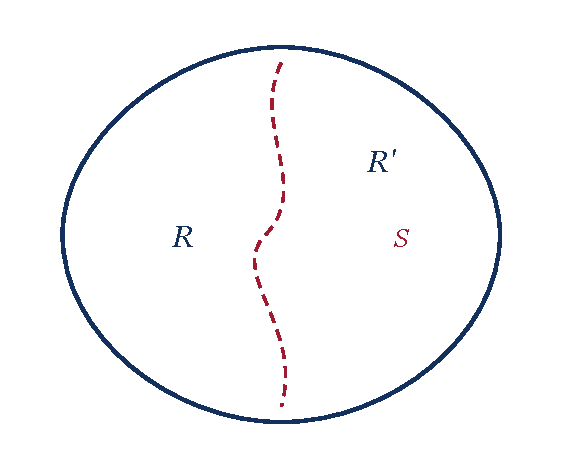
\includegraphics[width=0.6\textwidth]{figuras/pdf/cap01-fig1.pdf}
\caption{Un volumen del medio elástico dividido en dos partes $\mathrm{R}$
y $\mathrm{R}'$ por una superficie interior $S$.}
\label{fig:cap1-1}
\end{figure}

Este último potencial es muy pequeño. En efecto, las moléculas que
reaccionan unas sobre otras deben estar a una distancia menor que el radio
de la esfera de actividad molecular; por consiguiente, las moléculas del
volumen $\mathrm{R}$ que actúan sobre las del volumen $\mathrm{R}'$, y las
moléculas del volumen $\mathrm{R}'$ que actúan sobre las del volumen
$\mathrm{R}$, estarán comprendidas en el interior de un volumen limitado
por dos superficies paralelas a la superficie de separación de
$\mathrm{R}$ y de $\mathrm{R}'$, y situadas a una distancia de esta
superficie igual al radio de actividad molecular. Este volumen será
despreciable respecto de $\mathrm{R}$ y de $\mathrm{R}'$, y, si admitimos
que el número de moléculas de un medio es proporcional al volumen que
ocupan, las moléculas de cada uno de los volúmenes $\mathrm{R}$ y
$\mathrm{R}'$ que reaccionan sobre las moléculas del otro volumen serán en
número despreciable respecto de las moléculas contenidas en $\mathrm{R}$ o
en $\mathrm{R}'$. Por consiguiente, el potencial debido a la acción de las
moléculas del volumen $\mathrm{R}$ sobre las del volumen $\mathrm{R}'$
podrá despreciarse frente a $\mathrm{V}$ y $\mathrm{V}'$; tendremos:
\[
\mathrm{U}'=\mathrm{V}+\mathrm{V}'.
\]

Este razonamiento subsiste, por lo demás, si se divide el volumen ocupado
por el medio elástico en un número infinitamente grande de volúmenes
infinitamente pequeños, con tal de que las dimensiones de estos volúmenes
elementales sigan siendo infinitamente grandes respecto del radio de
actividad molecular; esto será siempre posible, puesto que este radio es un
infinitamente pequeño en valor absoluto. Designando por $d\tau$ uno de
estos elementos de volumen, por $\mathrm{W}\,d\tau$ el potencial debido a
las acciones mutuas de las moléculas situadas en el interior de este
elemento, el potencial de las fuerzas interiores del volumen total será:
\begin{equation}
\mathrm{U}'=\int \mathrm{W}\,d\tau.
\tag{16}
\end{equation}

\noindent\textbf{13.} Podemos desarrollar $\mathrm{W}$ según las potencias
crecientes de las $\xi$ y, despreciando los términos de grado superior al
segundo, tendremos:
\[
\mathrm{W}=\mathrm{W}_0+\mathrm{W}_1+\mathrm{W}_2.
\]
El término constante $\mathrm{W}_0$ puede suponerse nulo, y la relación
(16) nos dará:
\begin{equation}
\mathrm{U}'_1=\int \mathrm{W}_1\,d\tau,
\tag{17}
\end{equation}
\begin{equation}
\mathrm{U}'_2=\int \mathrm{W}_2\,d\tau.
\tag{18}
\end{equation}
La función de fuerzas $\mathrm{U}$ que entra en las ecuaciones del
movimiento se convertirá, teniendo en cuenta la relación (7), en:
\begin{equation}
\mathrm{U}=\mathrm{U}''_2+\int \mathrm{W}_2\,d\tau.
\tag{19}
\end{equation}

También podemos desarrollar la función $\mathrm{W}$ según las potencias
crecientes de las $\rho$, como lo hicimos para la función $\mathrm{U}'$; y,
remitiéndonos a la fórmula (15), escribiremos:
\begin{equation}
\mathrm{W}_2=\sum\frac{d\mathrm{F}}{d\mathrm{R}}\rho_2
+\frac12\sum\frac{d^2\mathrm{F}}{d\mathrm{R}^2}\rho_1^2
+\sum\frac{d^2\mathrm{F}}{d\mathrm{R}\,d\mathrm{R}'}\rho_1\rho_1',
\tag{20}
\end{equation}
extendiéndose la suma únicamente a las moléculas del elemento $d\tau$.
Siendo la cantidad $\rho_1$ homogénea y lineal respecto de las cantidades
$\mathrm{D}\xi,\mathrm{D}\eta,\mathrm{D}\zeta$, y $\rho_2$ homogénea y de
segundo grado respecto de esas mismas cantidades, resulta de la expresión
precedente que $\mathrm{W}_2$ es una función homogénea y de segundo grado
de $\mathrm{D}\xi,\mathrm{D}\eta,\mathrm{D}\zeta$.

\noindent\textbf{14. Nuevas hipótesis.} — Admitiremos que los
desplazamientos $\xi,\eta,\zeta$ son funciones continuas de las coordenadas
$x,y,z$ de la molécula en la posición de equilibrio, y que lo mismo ocurre
con sus derivadas sucesivas. Esta hipótesis es legítima, pues, si fuera de
otro modo, y si el desplazamiento relativo de dos moléculas muy vecinas no
fuera muy pequeño, resultarían de ello reacciones elásticas muy
considerables que no permitirían subsistir un estado de cosas semejante.

Admitida la continuidad de las funciones $\xi,\eta,\zeta$ y de sus
derivadas, podemos desarrollar estas funciones según las potencias
crecientes de las variables $x,y,z$, y tendremos:
\[
\mathrm{D}\xi=\frac{d\xi}{dx}\mathrm{D}x+\frac{d\xi}{dy}\mathrm{D}y+\frac{d\xi}{dz}\mathrm{D}z
+\frac12\left[\frac{d^2\xi}{dx^2}\mathrm{D}x^2+\frac{d^2\xi}{dy^2}\mathrm{D}y^2+\ldots\right]\ldots
\]
Las cantidades $\mathrm{D}x,\mathrm{D}y,\mathrm{D}z$, que son los
incrementos de las coordenadas al pasar de una molécula a una molécula
vecina, son del orden del radio de actividad molecular; los cuadrados de
estas cantidades serán infinitamente pequeños que en general se podrán
suprimir. Veremos sin embargo que no siempre tenemos el derecho de hacer
desaparecer estos cuadrados, y que una de las teorías propuestas para la
explicación de la dispersión de la luz necesita su conservación.
Suprimiéndolos, $\mathrm{D}\xi,\mathrm{D}\eta,\mathrm{D}\zeta$ vienen dados
por funciones lineales y homogéneas de las nueve derivadas parciales
\[
\frac{d\xi}{dx},\;\frac{d\xi}{dy},\;\frac{d\xi}{dz},\;\frac{d\eta}{dx},\ldots
\]
Se tiene:
\begin{equation}
\begin{gathered}
\mathrm{D}\xi=\frac{d\xi}{dx}\mathrm{D}x+\frac{d\xi}{dy}\mathrm{D}y+\frac{d\xi}{dz}\mathrm{D}z,\\
\mathrm{D}\eta=\frac{d\eta}{dx}\mathrm{D}x+\frac{d\eta}{dy}\mathrm{D}y+\frac{d\eta}{dz}\mathrm{D}z,\\
\mathrm{D}\zeta=\frac{d\zeta}{dx}\mathrm{D}x+\frac{d\zeta}{dy}\mathrm{D}y+\frac{d\zeta}{dz}\mathrm{D}z.
\end{gathered}
\tag{21}
\end{equation}

\noindent\textbf{15. Estudio de la función $\mathrm{W}_2$.} — Hemos visto
(§13) que $\mathrm{W}_2$ era una función homogénea de segundo grado
respecto a las cantidades $\mathrm{D}\xi,\mathrm{D}\eta,\mathrm{D}\zeta$;
es, pues, también una función homogénea y de segundo orden respecto a las
nueve derivadas parciales $\dfrac{d\xi}{dx},\dfrac{d\xi}{dy},\ldots$,
derivadas que en adelante representaremos a menudo con la notación de
Lagrange: $\xi'_x,\xi'_y,\xi'_z,\ldots$. Una forma cuadrática con nueve
variables independientes contiene nueve términos cuadrados y un número de
términos rectangulares igual al número de combinaciones de nueve objetos
tomados de dos en dos: $\dfrac{9\times 8}{2}=36$; puede, pues, contener
cuarenta y cinco coeficientes arbitrarios. Vamos a buscar el número de
coeficientes de la función $\mathrm{W}_2$.

Consideremos primero el término $\displaystyle\sum\frac{d\mathrm{F}}{d\mathrm{R}}\rho_2$
de esta función, desarrollado según la fórmula (20). Los términos en
$\xi_x'^2$ que entran en $\displaystyle\sum\frac{d\mathrm{F}}{d\mathrm{R}}\rho_2$
solo pueden provenir de $\mathrm{D}\xi^2$, pues ni $\mathrm{D}\eta$ ni
$\mathrm{D}\zeta$ contienen $\xi'_x$. Ahora bien, se tiene, elevando al
cuadrado los dos miembros de la primera de las relaciones (21):
\[
\mathrm{D}\xi^2=\left(\frac{d\xi}{dx}\right)^2\mathrm{D}x^2
+\left(\frac{d\xi}{dy}\right)^2\mathrm{D}y^2+\left(\frac{d\xi}{dz}\right)^2\mathrm{D}z^2
+2\frac{d\xi}{dx}\frac{d\xi}{dy}\mathrm{D}x\,\mathrm{D}y+\ldots;
\]
y el coeficiente de $\xi_x'^2$ en $\displaystyle\sum\frac{d\mathrm{F}}{d\mathrm{R}}\rho_2$ es:
\[
\sum\frac{d\mathrm{F}}{d\mathrm{R}}\mathrm{D}x^2.
\]
Se encontraría la misma cantidad para el coeficiente de $\eta_x'^2$ y de
$\zeta_x'^2$. Los coeficientes de los cuadrados de las nueve derivadas
parciales se reducen, pues, a tres:
\[
\sum\frac{d\mathrm{F}}{d\mathrm{R}}\mathrm{D}x^2,\qquad
\sum\frac{d\mathrm{F}}{d\mathrm{R}}\mathrm{D}y^2,\qquad
\sum\frac{d\mathrm{F}}{d\mathrm{R}}\mathrm{D}z^2.
\]
El coeficiente del doble producto $2\dfrac{d\xi}{dx}\dfrac{d\xi}{dy}$ es
$\displaystyle\sum\frac{d\mathrm{F}}{d\mathrm{R}}\mathrm{D}x\,\mathrm{D}y$.
Es fácil ver, desarrollando los cuadrados de $\mathrm{D}\eta$ y de
$\mathrm{D}\zeta$, que los productos $2\dfrac{d\eta}{dx}\dfrac{d\eta}{dy}$,
$2\dfrac{d\zeta}{dx}\dfrac{d\zeta}{dy}$, tienen por coeficientes esta misma
cantidad. Los coeficientes de los nueve dobles productos que entran en
$\displaystyle\sum\frac{d\mathrm{F}}{d\mathrm{R}}\rho_2$ se reducen, pues, a
los tres siguientes:
\[
\sum\frac{d\mathrm{F}}{d\mathrm{R}}\mathrm{D}x\,\mathrm{D}y,\qquad
\sum\frac{d\mathrm{F}}{d\mathrm{R}}\mathrm{D}y\,\mathrm{D}z,\qquad
\sum\frac{d\mathrm{F}}{d\mathrm{R}}\mathrm{D}z\,\mathrm{D}x.
\]
Por consiguiente, el primer término de $\mathrm{W}_2$ no contiene más que
seis coeficientes arbitrarios. Estos seis coeficientes son nulos cuando se
supone la presión exterior nula en el estado de equilibrio, según lo
establecido en el §10.

\noindent\textbf{16.} Los dos últimos términos de $\mathrm{W}_2$ son
homogéneos en $\rho_1$ y $\rho_1'$. Reemplazando, en la expresión de
$\rho_1$,
\[
\rho_1=2(\mathrm{D}x\,\mathrm{D}\xi+\mathrm{D}y\,\mathrm{D}\eta+\mathrm{D}z\,\mathrm{D}\zeta),
\]
$\mathrm{D}\xi,\mathrm{D}\eta,\mathrm{D}\zeta$ por sus valores (21), se
encuentra:
\begin{equation}
\begin{split}
\tfrac12\rho_1={}&\frac{d\xi}{dx}\mathrm{D}x^2+\frac{d\eta}{dy}\mathrm{D}y^2+\frac{d\zeta}{dz}\mathrm{D}z^2
+\left(\frac{d\xi}{dy}+\frac{d\eta}{dx}\right)\mathrm{D}x\,\mathrm{D}y\\
&+\left(\frac{d\eta}{dz}+\frac{d\zeta}{dy}\right)\mathrm{D}y\,\mathrm{D}z
+\left(\frac{d\zeta}{dx}+\frac{d\xi}{dz}\right)\mathrm{D}z\,\mathrm{D}x;
\end{split}
\tag{22}
\end{equation}
es decir, que $\rho_1$ es una función lineal y homogénea de las seis
cantidades
\[
\frac{d\xi}{dx},\quad \frac{d\eta}{dy},\quad \frac{d\zeta}{dz},\quad
\frac{d\xi}{dy}+\frac{d\eta}{dx},\quad \frac{d\eta}{dz}+\frac{d\zeta}{dy},\quad
\frac{d\zeta}{dx}+\frac{d\xi}{dz}.
\]
La suma de los dos últimos términos de $\mathrm{W}_2$
es, pues, una función homogénea y de segundo grado de estas seis
cantidades; por consiguiente, no contendrá más que $21$ coeficientes
arbitrarios ($6$ coeficientes para los cuadrados y $15$ para los dobles
productos).

\noindent\textbf{17.} Vemos ya que, en el caso más general, la función $\mathrm{W}_2$ no
contendrá más que $21+6=27$ coeficientes arbitrarios, número que se
reducirá a $21$ cuando la presión exterior sea nula en el estado de
equilibrio.

En la hipótesis de las fuerzas centrales, hemos visto (§11) que se tenía:
\[
\frac{d^2\mathrm{F}}{d\mathrm{R}\,d\mathrm{R}'}=0.
\]
El tercer término del desarrollo (20) de $\mathrm{W}_2$ desaparece
entonces, y, si en el segundo término reemplazamos $\rho_1^2$ por su valor
tomado de la relación (22), se comprueba que, entre los 21 coeficientes,
seis son iguales dos a dos. Así se tiene:
\[
\text{coef. de }\left(\frac{d\xi}{dy}+\frac{d\eta}{dx}\right)^2
=\text{coef. de }2\frac{d\xi}{dx}\frac{d\eta}{dy},
\]
\[
\text{coef. de }2\frac{d\zeta}{dz}\left(\frac{d\xi}{dy}+\frac{d\eta}{dx}\right)
=\text{coef. de }2\left(\frac{d\eta}{dz}+\frac{d\zeta}{dy}\right)\left(\frac{d\zeta}{dx}+\frac{d\xi}{dz}\right).
\]
El número de coeficientes arbitrarios se encuentra entonces reducido a 15.

En resumen, tendremos en $\mathrm{W}_2$: 1.\textsuperscript{o} 27
coeficientes arbitrarios en el caso general; 2.\textsuperscript{o} 21
coeficientes cuando la presión exterior es nula en el estado de equilibrio
y las fuerzas no son centrales; 3.\textsuperscript{o} 21 coeficientes
cuando las fuerzas son centrales y la presión exterior es distinta de cero
en el estado de equilibrio (hipótesis de Cauchy); 4.\textsuperscript{o} 15
coeficientes cuando las fuerzas son centrales y la presión exterior es
nula en el estado de equilibrio.

El valor de estos coeficientes, en un medio cualquiera, dependerá en
general de las coordenadas del centro de gravedad del elemento de volumen
$d\tau$. Para simplificar la cuestión y situarnos en el caso más corriente,
supondremos el medio homogéneo: los coeficientes se convertirán en
constantes.

\section{Funciones isótropas}

\noindent\textbf{18.} Un medio homogéneo se dice isótropo cuando, en ese
medio, todas las direcciones son idénticas. El éter en el vacío, los
cuerpos gaseosos, los líquidos, los sólidos amorfos son isótropos; los
sólidos cristalizados no lo son. De esta definición resulta que, en un
cuerpo isótropo, un plano cualquiera es un plano de simetría; en
particular, los planos de coordenadas son planos de simetría. Las
ecuaciones del movimiento y, por consiguiente, la función $\mathrm{W}_2$,
no deben cambiar cuando se sustituye $-x$ en lugar de $x$ y $-\xi$ en
lugar de $\xi$, o $-y$ en lugar de $y$ y $-\eta$ en lugar de $\eta$, o
finalmente $-z$ en lugar de $z$ y $-\zeta$ en lugar de $\zeta$.
Observaremos, por lo demás, que los cuerpos isótropos no son los únicos
que gozan de esta propiedad; pertenece a todos los cuerpos cristalizados
que poseen tres planos de simetría rectangulares, es decir, a los cuerpos
cristalizados pertenecientes a los cuatro primeros sistemas cristalinos.
Para estos cuerpos y para los isótropos, la función $\mathrm{W}_2$ no debe
contener términos que cambien de signo por alguna de las tres sustituciones
precedentes; es fácil reconocer que los términos que pueden subsistir
forman cuatro grupos: 1.\textsuperscript{o} los términos cuadrados de la
forma $\dfrac{d\xi^2}{dx^2}$; 2.\textsuperscript{o} los de la forma $\dfrac{d\xi^2}{dy^2}$;
3.\textsuperscript{o} los términos rectangulares tales como
$\dfrac{d\xi}{dx}\dfrac{d\eta}{dy}$; 4.\textsuperscript{o} el término
$\dfrac{d\xi}{dy}\dfrac{d\eta}{dx}$ y los que de él se deducen por
permutación.

Dentro de los cuerpos isótropos y de los cuerpos cristalizados del sistema
cúbico, todos los términos de un mismo grupo tienen el mismo coeficiente.
En efecto, en esos cuerpos las tres direcciones de los ejes de coordenadas
desempeñan el mismo papel; por consiguiente, podemos permutar dos de los
ejes, o los tres ejes, sin cambiar $\mathrm{W}_2$, es decir que
$\mathrm{W}_2$ debe conservar el mismo valor cuando en ella se permutan,
por ejemplo, $x$ e $y$, $\xi$ y $\eta$. Para que así sea, es necesario que
los coeficientes de los términos $\dfrac{d\xi^2}{dx^2},\dfrac{d\eta^2}{dy^2},
\dfrac{d\zeta^2}{dz^2}$ sean los mismos; por consiguiente, los términos del
primer grupo entran en la función $\mathrm{W}_2$ por su suma:\footnote{Corrección
indicada en la fe de erratas del propio volumen original (p.~21,
línea~13), que pide leer $d\eta^2/dy^2$ en lugar de $dy^2/dy^2$ en el
segundo término.~(N.~del T.)}
\[
\frac{d\xi^2}{dx^2}+\frac{d\eta^2}{dy^2}+\frac{d\zeta^2}{dz^2}.
\]
Como ocurre lo mismo para los términos de los otros tres grupos, la función
$\mathrm{W}_2$ es la suma de cuatro polinomios, homogéneos y de segundo
grado respecto a las nueve derivadas parciales, multiplicados
respectivamente por coeficientes numéricos. Estos cuatro polinomios son:
\[
\xi_x'^2+\eta_y'^2+\zeta_z'^2
\]
\[
\xi_y'^2+\xi_z'^2+\eta_x'^2+\eta_z'^2+\zeta_x'^2+\zeta_y'^2
\]
\[
\xi_x'\eta_y'+\xi_x'\zeta_z'+\eta_y'\zeta_z'
\]
\[
\xi_y'\eta_x'+\xi_z'\zeta_x'+\eta_z'\zeta_y'.
\]

\noindent\textbf{19.} Queda por averiguar si estos cuatro polinomios
independientes subsistirán en el caso de un cuerpo perfectamente isótropo.
Vamos a mostrar que se reducen a tres, que llamaremos polinomios isótropos.

Puesto que en un cuerpo isótropo todas las direcciones son idénticas, la
expresión de un polinomio isótropo no debe cambiar cuando se hace un cambio
cualquiera de coordenadas conservando el mismo origen; la forma de un
polinomio isótropo debe ser independiente de la elección de los ejes.

Sean $x,y,z$ las coordenadas de una molécula $\mu$ (figura~\ref{fig:cap1-2})
de un medio isótropo; $x+\mathrm{D}x,\,y+\mathrm{D}y,\,z+\mathrm{D}z$ las de
una molécula vecina $\mu'$. Cuando la molécula $\mu$ sea desplazada de su
posición de equilibrio, vendrá a $\mu_1$, cuyas coordenadas son
$x+\xi,\,y+\eta,\,z+\zeta$; la molécula $\mu'$ ocupará el punto $\mu'_1$ de
coordenadas $x+\xi+\mathrm{D}x+\mathrm{D}\xi,\,y+\eta+\mathrm{D}y+\mathrm{D}\eta,
\,z+\zeta+\mathrm{D}z+\mathrm{D}\zeta$. Por el punto $\mu$ tracemos la recta
$\mu\mu''$ igual y paralela a $\mu_1\mu'_1$, y unamos $\mu'$ a $\mu''$. Por
el punto $\mathrm{O}$, origen de las coordenadas, tracemos una recta
$\mathrm{OM}$ igual y paralela a $\mu\mu'$ y una recta $\mathrm{OP}$ igual y
paralela a $\mu'\mu''$; las coordenadas del punto $\mathrm{M}$ serán
$\mathrm{D}x,\mathrm{D}y,\mathrm{D}z$; las del punto $\mathrm{P}$ serán
$\mathrm{D}\xi,\mathrm{D}\eta,\mathrm{D}\zeta$.

\begin{figure}[ht]
\centering
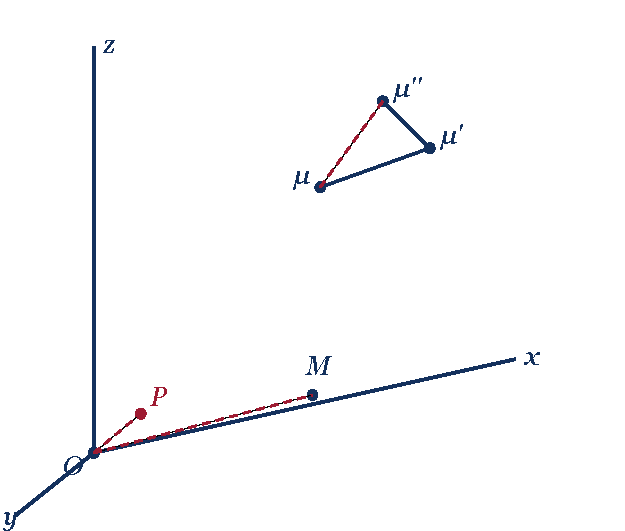
\includegraphics[width=0.75\textwidth]{figuras/pdf/cap01-fig2.pdf}
\caption{Construcción geométrica del §19: los puntos $\mu,\mu',\mu''$ y los
segmentos $\mathrm{OM}$, $\mathrm{OP}$, iguales y paralelos a $\mu\mu'$ y
$\mu'\mu''$.}
\label{fig:cap1-2}
\end{figure}

Designando por $l$ la longitud de la recta $\mathrm{OP}$, tendremos:
\begin{equation}
l^2=\mathrm{D}\xi^2+\mathrm{D}\eta^2+\mathrm{D}\zeta^2,
\tag{23}
\end{equation}
y, como, según las ecuaciones (21), $\mathrm{D}\xi,\mathrm{D}\eta,\mathrm{D}\zeta$
son funciones homogéneas y de primer grado respecto a $\mathrm{D}x,\mathrm{D}y,
\mathrm{D}z$, $l^2$ es una función homogénea y de segundo grado respecto a
las coordenadas del punto $\mathrm{M}$. Por consiguiente, el lugar de los
puntos $\mathrm{M}$ tales que la longitud $\mathrm{OP}$ permanezca
constante es un elipsoide cuyo centro está en $\mathrm{O}$. Siendo isótropo
el medio, debe encontrarse el mismo elipsoide cualquiera que sea la
dirección de los ejes. La ecuación del elipsoide dependerá naturalmente de
la elección de los ejes; pero el elipsoide mismo no cambiará cuando se
cambien los tres planos de coordenadas. Ahora bien, se sabe que, si un
elipsoide es fijo en el espacio, existen ciertas funciones de los
coeficientes de su ecuación, conocidas con el nombre de invariantes, que
son independientes de la elección de los ejes; ellas deberán ser funciones
isótropas. Uno de los invariantes es la suma de los cuadrados de los
coeficientes de los términos cuadrados. Para hallarlo, reemplacemos en la
ecuación (23) las cantidades $\mathrm{D}\xi,\mathrm{D}\eta,\mathrm{D}\zeta$
por los valores (21). Tendremos entre las coordenadas $\mathrm{D}x,\mathrm{D}y,
\mathrm{D}z$ del punto $\mathrm{M}$ una relación que será precisamente la
ecuación de nuestro elipsoide, y obtendremos para el coeficiente de
$\mathrm{D}x^2$ la suma:
\[
\xi_x'^2+\eta_x'^2+\zeta_x'^2;
\]
el de $\mathrm{D}y^2$ será:
\[
\xi_y'^2+\eta_y'^2+\zeta_y'^2;
\]
y el de $\mathrm{D}z^2$:
\[
\xi_z'^2+\eta_z'^2+\zeta_z'^2.
\]
La suma de estos tres coeficientes será, pues, una función isótropa. La
designaremos por $\mathrm{H}$; será la suma de los cuadrados de las nueve
derivadas parciales:
\begin{equation}
\mathrm{H}=\sum \xi_x'^2.
\tag{24}
\end{equation}

\noindent\textbf{20.} Para hallar otras funciones isótropas, consideremos
el caso en que las moléculas $\mu$ y $\mu'$ se desplazan de manera que la
recta $\mu\mu'$ permanezca siempre paralela a sí misma: las rectas
$\mathrm{OP}$ y $\mathrm{OM}$ son paralelas, y, designando por $\alpha$ la
razón de sus longitudes, se tiene:
\[
\mathrm{D}\xi=\alpha\,\mathrm{D}x,\qquad \mathrm{D}\eta=\alpha\,\mathrm{D}y,
\qquad \mathrm{D}\zeta=\alpha\,\mathrm{D}z.
\]
Si se llevan estos valores a las ecuaciones (21) del §14, se obtiene:
\[
\alpha\,\mathrm{D}x=\xi_x'\,\mathrm{D}x+\xi_y'\,\mathrm{D}y+\xi_z'\,\mathrm{D}z,
\]
\[
\alpha\,\mathrm{D}y=\eta_x'\,\mathrm{D}x+\eta_y'\,\mathrm{D}y+\eta_z'\,\mathrm{D}z,
\]
\[
\alpha\,\mathrm{D}z=\zeta_x'\,\mathrm{D}x+\zeta_y'\,\mathrm{D}y+\zeta_z'\,\mathrm{D}z,
\]
y la eliminación de $\mathrm{D}x,\mathrm{D}y,\mathrm{D}z$ entre estas
ecuaciones conduce al determinante:
\[
\begin{vmatrix}
\xi_x'-\alpha & \xi_y' & \xi_z'\\
\eta_x' & \eta_y'-\alpha & \eta_z'\\
\zeta_x' & \zeta_y' & \zeta_z'-\alpha
\end{vmatrix}=0.
\]
Esta ecuación determinará $\alpha$. Ahora bien, esta cantidad es
evidentemente independiente de la elección de los ejes de coordenadas; por
consiguiente, los coeficientes de esta ecuación en $\alpha$ son
invariantes. El coeficiente del término en $\alpha^2$ es:
\[
\xi_x'+\eta_y'+\zeta_z'.
\]
Designaremos esta nueva función isótropa por $\Theta$, y, como entrará en
segundo grado en la función $\mathrm{W}_2$, consideraremos su cuadrado:
\begin{equation}
\Theta^2=(\xi_x'+\eta_y'+\zeta_z')^2.
\tag{25}
\end{equation}

\noindent\textbf{21.} Esta función $\Theta$ tiene una significación
geométrica interesante.

El volumen de una porción del medio elástico en su posición de equilibrio
tiene por expresión:
\[
\iiint dx\,dy\,dz.
\]
A causa de la deformación del medio, las coordenadas del centro de
gravedad de cada elemento del volumen se convierten en $x+\xi,\,y+\eta,
\,z+\zeta$, y el volumen de la porción considerada toma el valor:
\[
\iiint (dx+d\xi)(dy+d\eta)(dz+d\zeta).
\]
Recordemos que, si se tiene una integral
\[
\iiint \mathrm{F}(x,y,z)\,dx\,dy\,dz
\]
donde $x,y,z$ son funciones de tres nuevas variables $\alpha,\beta,\gamma$,
esta integral se convierte, al tomar como variables $\alpha,\beta,\gamma$,
en
\[
\iiint \Phi(\alpha,\beta,\gamma)\,\frac{\mathrm{D}(x,y,z)}{\mathrm{D}(\alpha,\beta,\gamma)}\,d\alpha\,d\beta\,d\gamma,
\]
designando $\mathrm{D}(x,y,z)/\mathrm{D}(\alpha,\beta,\gamma)$ el
determinante funcional\footnote{Es lo que hoy se llama el \emph{jacobiano}
de $x,y,z$ respecto a $\alpha,\beta,\gamma$.~(N.~del T.)} de $x,y,z$ respecto a
$\alpha,\beta,\gamma$. Apoyándonos en este teorema, tendremos,
para la expresión del volumen después de la deformación:
\[
\iiint \frac{\mathrm{D}[(x+\xi),(y+\eta),(z+\zeta)]}{\mathrm{D}(x,y,z)}\,dx\,dy\,dz.
\]
El determinante funcional que entra en esta integral tiene por valor:
\[
\begin{vmatrix}
1+\xi_x' & \xi_y' & \xi_z'\\
\eta_x' & 1+\eta_y' & \eta_z'\\
\zeta_x' & \zeta_y' & 1+\zeta_z'
\end{vmatrix}
\]
y, si, en el desarrollo de este determinante, se desprecian las potencias
de las derivadas que son superiores al primer grado, se obtiene:
\[
1+\xi_x'+\eta_y'+\zeta_z',
\]
es decir:
\[
1+\Theta.
\]
Si llevamos este valor del determinante funcional a la integral que da el
volumen después de la deformación, obtenemos:
\[
\iiint (1+\Theta)\,dx\,dy\,dz.
\]
Un elemento de volumen $dx\,dy\,dz$ se convierte, pues, después de la
deformación, en $(1+\Theta)\,dx\,dy\,dz$; por consiguiente, $\Theta$ es el
coeficiente de dilatación cúbica del medio.

\noindent\textbf{22.} Volvamos a nuestra ecuación en $\alpha$. El
coeficiente del término en $-\alpha$ es:
\begin{equation}
\mathrm{K}=\xi_x'\eta_y'-\xi_y'\eta_x'+\eta_y'\zeta_z'-\eta_z'\zeta_y'+\zeta_z'\xi_x'-\zeta_x'\xi_z'.
\tag{26}
\end{equation}
Es un tercer polinomio isótropo, que puede escribirse:
\[
\mathrm{K}=\frac{\mathrm{D}(\xi,\eta)}{\mathrm{D}(x,y)}+\frac{\mathrm{D}(\eta,\zeta)}{\mathrm{D}(y,z)}+\frac{\mathrm{D}(\zeta,\xi)}{\mathrm{D}(z,x)}.
\]

\noindent\textbf{23.} Los tres polinomios isótropos de segundo grado,
$\mathrm{H},\Theta^2,\mathrm{K}$, son tres polinomios independientes. No
puede haber otros, pues, si hubiera cuatro, todos los cuerpos que gozan de
la simetría cúbica —para la cual la función $\mathrm{W}_2$ es una suma de
cuatro polinomios de segundo grado e independientes— gozarían al mismo
tiempo de la isotropía. Por lo demás, el primero de los polinomios que
entra en $\mathrm{W}_2$, en el caso de los cuerpos de simetría cúbica (§18):
\[
\xi_x'^2+\eta_y'^2+\zeta_z'^2
\]
no es un polinomio isótropo, pues cambia cuando se hacen girar los ejes,
como es fácil convencerse haciendo girar los ejes de las $x$ y de las $y$
en $45^\circ$ en el plano de las $xy$.

\section{Expresión de \texorpdfstring{$\mathrm{W}_2$}{W₂} en el caso de los cuerpos isótropos}

\noindent\textbf{24.} La función $\mathrm{W}_2$ no puede contener más que
los tres polinomios isótropos que acabamos de hallar, y, como esta función
es homogénea y de segundo grado respecto a las nueve derivadas parciales
$\xi_x',\xi_y',\ldots$, debe ser lineal y homogénea respecto a los tres
polinomios isótropos, que son ellos mismos homogéneos y de segundo grado
respecto a las nueve derivadas parciales; será de la forma:
\begin{equation}
\mathrm{W}_2=\lambda\mathrm{K}+\mu\mathrm{H}+\nu\Theta^2.
\tag{27}
\end{equation}

Comparemos esta expresión con el desarrollo (20) de esta misma función. El
primer término de este desarrollo y el conjunto de los dos últimos deberán
ser separadamente isótropos, pues, en un medio isótropo, toda función
simétrica de las distancias mutuas de los puntos ocupados por las
moléculas antes y después del desplazamiento debe ser una función isótropa.

Consideremos primero el término $\displaystyle\sum\frac{d\mathrm{F}}{d\mathrm{R}}\rho_2$
de esta expresión; vamos a demostrar que es igual al polinomio $\mathrm{H}$
multiplicado por un factor constante.

En el estudio de la función $\mathrm{W}_2$ (§15) hemos visto que, si
reemplazamos en el primer término del desarrollo de esta función las
cantidades $\mathrm{D}\xi,\mathrm{D}\eta,\mathrm{D}\zeta$ por sus valores
dados por las relaciones (21), obtenemos para este término un polinomio
homogéneo y de segundo grado respecto a las nueve derivadas parciales,
que contiene los cuadrados de estas derivadas y los nueve dobles productos
de la forma $\dfrac{d\xi}{dx}\dfrac{d\xi}{dy}$. Pero este término, siendo
una función isótropa, no puede contener esos dobles productos, que no
entran en ninguno de los cuatro grupos de términos que subsisten en el caso
de los cuerpos de simetría cúbica (§18); el primer término de $\mathrm{W}_2$
se reduce, pues, a un polinomio que no contiene más que los cuadrados de
las derivadas parciales. No puede contener ni $\Theta$ ni $\mathrm{K}$,
pues en la función $\mathrm{K}$ se encuentran dobles productos tales como
$\xi_y'\eta_x'$ que no pueden reducirse con los dobles productos de
$\Theta^2$, que no son de esta forma. Debemos, pues, tener:
\begin{equation}
\sum\frac{d\mathrm{F}}{d\mathrm{R}}\rho_2=\mu_1\mathrm{H}.
\tag{28}
\end{equation}

\noindent\textbf{25.} El conjunto de los dos últimos términos:
\[
\frac12\sum\frac{d^2\mathrm{F}}{d\mathrm{R}^2}\rho_1^2
+\sum\frac{d^2\mathrm{F}}{d\mathrm{R}\,d\mathrm{R}'}\rho_1\rho_1'
\]
del desarrollo (20) de la función $\mathrm{W}_2$ es también, en el caso de
los cuerpos isótropos, una función isótropa, y de las relaciones (20) (27)
y (28) deducimos la igualdad:
\begin{equation}
\frac12\sum\frac{d^2\mathrm{F}}{d\mathrm{R}^2}\rho_1^2
+\sum\frac{d^2\mathrm{F}}{d\mathrm{R}\,d\mathrm{R}'}\rho_1\rho_1'
=\lambda\mathrm{K}+(\mu-\mu_1)\mathrm{H}+\nu\Theta^2.
\tag{29}
\end{equation}

En el estudio de la función $\mathrm{W}_2$ (§16) hemos mostrado que, en
el caso general, el primer miembro de esta igualdad es una función homogénea y de segundo
grado de las seis cantidades:
\[
\xi_x',\quad \eta_y',\quad \zeta_z',
\]
\[
\xi_y'+\eta_x',\quad \eta_z'+\zeta_y',\quad \zeta_x'+\xi_z'.
\]
Los términos $\xi_y'^2$ y $2\xi_y'\eta_x'$ solo pueden provenir del
cuadrado de la cantidad $\xi_y'+\eta_x'$; por consiguiente, estos términos
deben tener el mismo coeficiente. Ahora bien, el término $\xi_y'^2$ no se
encuentra más que en la función $\mathrm{H}$, donde tiene el coeficiente
$1$; entrará, pues, en el segundo miembro de la relación (29) con el
coeficiente $\mu-\mu_1$.

El término $2\xi_y'\eta_x'$ no puede provenir más que
de la función $\mathrm{K}$, donde tiene el coeficiente $-\tfrac12$; su
coeficiente, en el segundo miembro de (29), será, pues, $-\tfrac{\lambda}{2}$.
Teniendo los dos términos considerados el mismo coeficiente en el primer
miembro de la relación, debe ocurrir lo mismo en el segundo miembro; por
consiguiente tendremos:
\begin{equation}
\mu-\mu_1=-\frac{\lambda}{2}.
\tag{30}
\end{equation}

\noindent\textbf{26.} Cuando se supone que la presión exterior es nula en el estado de
equilibrio, el término $\displaystyle\sum\frac{d\mathrm{F}}{d\mathrm{R}}\rho_2$
del desarrollo (20) desaparece (§15); por consiguiente, $\mu_1$ es nulo, y
la relación precedente se convierte en:
\begin{equation}
\mu=-\frac{\lambda}{2}.
\tag{31}
\end{equation}
No queda entonces más que dos coeficientes arbitrarios en la función
$\mathrm{W}_2$.

En la hipótesis de las fuerzas centrales, el término
$\displaystyle\sum\frac{d^2\mathrm{F}}{d\mathrm{R}\,d\mathrm{R}'}\rho_1\rho_1'$
es nulo (§17), y el primer miembro de la relación (29) se reduce a
$\tfrac12\displaystyle\sum\frac{d^2\mathrm{F}}{d\mathrm{R}^2}\rho_1^2$.
Ahora bien, hemos visto que, si se reemplaza $\rho_1^2$ por su valor
tomado de la relación (22), se obtenía:
\[
\text{coef. de }\left(\frac{d\xi}{dy}+\frac{d\eta}{dx}\right)^2
=\text{coef. de }2\frac{d\xi}{dx}\frac{d\eta}{dy};
\]
por consiguiente, el coeficiente de $\xi_y'^2$ debe ser igual al de
$2\xi_x'\eta_y'$ en el primer miembro de la igualdad (29), y debe ocurrir
lo mismo en el segundo miembro. El término $\xi_y'^2$ se encuentra en él
con el coeficiente $\mu-\mu_1$; el término $2\xi_x'\eta_y'$, que entra en
$\Theta^2$ con el coeficiente $1$ y en $\mathrm{K}$ con el coeficiente
$\tfrac12$, está en el segundo miembro de (29) con el coeficiente
$\nu+\tfrac{\lambda}{2}$. Por consiguiente, se tiene la relación:
\[
\mu-\mu_1=\nu+\frac{\lambda}{2}.
\]
Reemplazando en ella $\mu-\mu_1$ por su valor dado por (30), se obtiene:
\begin{equation}
\lambda+\nu=0;
\tag{32}
\end{equation}
y el número de coeficientes arbitrarios se encuentra reducido a dos.

\noindent\textbf{27.} En resumen, la función $\mathrm{W}_2$ relativa a las
fuerzas interiores que resultan de la deformación de un medio isótropo es
una función homogénea y de segundo grado de las nueve derivadas de las
cantidades $\xi$, que contiene a lo más tres coeficientes arbitrarios
$\lambda,\mu,\nu$. El número de estos coeficientes puede reducirse, en
ciertos casos particulares; tendremos:

1.\textsuperscript{o} Tres coeficientes arbitrarios en el caso general;

2.\textsuperscript{o} Dos coeficientes cuando la presión exterior es nula
en el estado de equilibrio y las fuerzas no son centrales;

3.\textsuperscript{o} Dos coeficientes cuando las fuerzas son centrales y
la presión exterior es distinta de cero en el estado de equilibrio
(hipótesis de Cauchy);

4.\textsuperscript{o} Un solo coeficiente cuando las fuerzas son centrales
y la presión exterior es nula en el estado de equilibrio, pues, en este
caso, las relaciones (31) y (32) se verifican simultáneamente.

\section{Presiones exteriores. Ecuaciones del movimiento}

\noindent\textbf{28. Expresión de $\mathrm{W}_1$ en función de las
derivadas parciales.} — La función $\mathrm{W}_1$ es el término de primer
grado del desarrollo de la función $\mathrm{W}$ respecto a las potencias
crecientes de las $\xi$ (§13); esta última función puede, como la función
$\mathrm{U}'$, desarrollarse según las potencias crecientes de las $\rho$,
y, remitiéndonos a las relaciones (12) y (17), obtendremos:
\[
\mathrm{W}_1=\sum\frac{d\mathrm{F}}{d\mathrm{R}}\rho_1,
\]
extendiéndose la suma únicamente a las moléculas del elemento de volumen
$d\tau$. Reemplazando $\rho_1$ por su valor tomado de la relación (22), la
función $\mathrm{W}_1$ se convierte en:
\begin{multline*}
\frac12\mathrm{W}_1=\xi_x'\sum\frac{d\mathrm{F}}{d\mathrm{R}}\mathrm{D}x^2
+\eta_y'\sum\frac{d\mathrm{F}}{d\mathrm{R}}\mathrm{D}y^2
+\zeta_z'\sum\frac{d\mathrm{F}}{d\mathrm{R}}\mathrm{D}z^2\\
+(\xi_y'+\eta_x')\sum\frac{d\mathrm{F}}{d\mathrm{R}}\mathrm{D}x\,\mathrm{D}y+\ldots
\end{multline*}
Es, pues, una función homogénea y de primer grado respecto a las nueve
derivadas parciales.

\noindent\textbf{29. Presiones exteriores. — Ecuaciones del movimiento.} —
Consideremos una superficie cerrada $S$ (figura~\ref{fig:cap1-1}) que
divide el medio elástico en dos partes: una, $\mathrm{R}$, interior a la
superficie; la otra, $\mathrm{R}'$, exterior. Las diversas moléculas de
$\mathrm{R}'$ ejercen acciones sobre las moléculas de $\mathrm{R}$, pero,
siendo muy pequeño el radio de la esfera de actividad molecular, solo las
moléculas de $\mathrm{R}$ vecinas de la superficie están sometidas a las
acciones de $\mathrm{R}'$. Estas acciones pueden reemplazarse por un
sistema de fuerzas aplicadas a los elementos $d\omega$ de la superficie
$S$ y que, en general, actuarán oblicuamente sobre el elemento
considerado. Designaremos por
\[
\mathrm{P}_x\,d\omega,\qquad \mathrm{P}_y\,d\omega,\qquad \mathrm{P}_z\,d\omega,
\]
las componentes según los tres ejes de la presión que se ejerce sobre el
elemento $d\omega$; son las fuerzas exteriores al sistema, si solo se
considera el volumen $\mathrm{R}$ limitado por la superficie. La aplicación
del principio de d'Alembert y del principio de las velocidades virtuales a
este sistema nos va a permitir hallar los valores de las componentes de las
presiones y, al mismo tiempo, darnos una nueva forma de las ecuaciones del
movimiento.

Si $\rho$ es la densidad de un elemento de volumen $d\tau$ (en adelante la
letra $\rho$ se empleará exclusivamente en este sentido), la masa del
elemento es $\rho\,d\tau$, y las tres componentes de la fuerza de inercia
que hay que suponer aplicada a este elemento, para que, según el principio
de d'Alembert, este elemento pueda considerarse en equilibrio, son:
\[
-\rho\,d\tau\,\frac{d^2\xi}{dt^2},\qquad -\rho\,d\tau\,\frac{d^2\eta}{dt^2},
\qquad -\rho\,d\tau\,\frac{d^2\zeta}{dt^2}.
\]
Estando todos los elementos del volumen $\mathrm{R}$ en equilibrio bajo la
acción de las fuerzas efectivas y de las fuerzas de inercia, se podrá
aplicar a este volumen el principio de las velocidades virtuales: en un
sistema en equilibrio, la suma de los trabajos virtuales es nula.
Designando por $\mathrm{U}$ la función de fuerzas relativa a las fuerzas
interiores y exteriores a $\mathrm{R}$, la suma de los trabajos virtuales
de estas fuerzas es $\delta\mathrm{U}$; y, llamando $\delta\xi,\delta\eta,
\delta\zeta$ a las proyecciones del desplazamiento virtual de un elemento
$d\tau$, el trabajo virtual de la fuerza de inercia es:
\[
-\rho\,d\tau\left(\frac{d^2\xi}{dt^2}\delta\xi+\frac{d^2\eta}{dt^2}\delta\eta+\frac{d^2\zeta}{dt^2}\delta\zeta\right).
\]
La suma de los trabajos de todas las fuerzas de inercia será:
\[
-\int \rho\,d\tau\left(\frac{d^2\xi}{dt^2}\delta\xi+\frac{d^2\eta}{dt^2}\delta\eta+\frac{d^2\zeta}{dt^2}\delta\zeta\right);
\]
y, según el principio de las velocidades virtuales, se tendrá:
\begin{equation}
\delta\mathrm{U}-\int \rho\,d\tau\left(\frac{d^2\xi}{dt^2}\delta\xi+\frac{d^2\eta}{dt^2}\delta\eta+\frac{d^2\zeta}{dt^2}\delta\zeta\right)=0,
\tag{33}
\end{equation}
cualesquiera que sean $\delta\xi,\delta\eta,\delta\zeta$.

Observemos que, según la relación (19), tenemos:
\[
\delta\mathrm{U}=\delta\mathrm{U}''+\int\delta\mathrm{W}\,d\tau;
\]
siendo $\delta\mathrm{U}''$ la suma de los trabajos virtuales de las
fuerzas exteriores, es decir, de las presiones definidas anteriormente,
tendremos:
\[
\delta\mathrm{U}''=\int d\omega\,(\mathrm{P}_x\,\delta\xi+\mathrm{P}_y\,\delta\eta+\mathrm{P}_z\,\delta\zeta),
\]
extendiéndose la integral a toda la superficie $S$. Si se supone que las
componentes $\delta\eta$ y $\delta\zeta$ del desplazamiento son nulas, el
trabajo virtual de las fuerzas exteriores se reduce a:
\[
\delta\mathrm{U}''=\int d\omega\,\mathrm{P}_x\,\delta\xi.
\]

La función $\mathrm{W}$ relativa a las fuerzas
interiores es una función de las nueve derivadas parciales de las $\xi$.
Por efecto del desplazamiento virtual dado al sistema, cada una de estas
derivadas varía en general, pero, en el caso particular donde se tiene
$\delta\eta=\delta\zeta=0$, las únicas derivadas que cambian de valor son
$\xi_x',\xi_y',\xi_z'$.\footnote{Corrección indicada en la fe de erratas del
propio volumen original (p.~35, línea~4), que pide leer
$\xi_x',\xi_y',\xi_z'$ en lugar de $\xi_x,\xi_y,\xi_z$.~(N.~del T.)} Por consiguiente:
\[
\delta\mathrm{W}=\frac{d\mathrm{W}}{d\xi_x'}\delta\xi_x'+\frac{d\mathrm{W}}{d\xi_y'}\delta\xi_y'+\frac{d\mathrm{W}}{d\xi_z'}\delta\xi_z'
=\sum\frac{d\mathrm{W}}{d\xi_x'}\delta\xi_x'.
\]
Ahora bien, $\delta\xi_x'$, es decir $\delta\dfrac{d\xi}{dx}$, es igual a
$\dfrac{d}{dx}\delta\xi$, y la expresión de $\delta\mathrm{W}$ se convierte
en
\[
\delta\mathrm{W}=\sum\frac{d\mathrm{W}}{d\xi_x'}\frac{d}{dx}\delta\xi.
\]
Por consiguiente, se tiene:
\[
\delta\mathrm{U}=\int d\omega\,\mathrm{P}_x\,\delta\xi+\int d\tau\sum\frac{d\mathrm{W}}{d\xi_x'}\frac{d}{dx}\delta\xi,
\]
y, llevando este valor a la igualdad (33), donde se hace $\delta\eta=\delta\zeta=0$
en el término relativo a los trabajos de las fuerzas de inercia, se
obtiene:
\begin{equation}
\int d\omega\,\mathrm{P}_x\,\delta\xi+\int d\tau\sum\frac{d\mathrm{W}}{d\xi_x'}\frac{d}{dx}\delta\xi
-\int \rho\,d\tau\,\frac{d^2\xi}{dt^2}\,\delta\xi=0.
\tag{34}
\end{equation}

\noindent\textbf{30.} Hay que transformar ahora esta expresión, que
contiene a la vez $\delta\xi$ y la derivada de esta cantidad respecto a
$x$. Para ello nos apoyaremos en el siguiente lema, que sirve
ordinariamente para la demostración del teorema de Green en la teoría del
potencial:\footnote{Es el teorema de la divergencia (de
Gauss--Ostrogradski) escrito para una sola componente.~(N.~del T.)} dada una función $\mathrm{F}$ de las coordenadas
$x,y,z$ de un punto, la integral de la diferencial $\mathrm{F}\alpha\,d\omega$,
donde $\alpha$ es el primer coseno director de la normal al elemento
$d\omega$ de una superficie cerrada $S$, extendida esta integral a todos
los elementos de la superficie $S$, es igual a la integral de la
diferencial $\dfrac{d\mathrm{F}}{dx}\,d\tau$, extendida a todos los
elementos $d\tau$ del volumen $\mathrm{R}$ limitado por la superficie $S$.

Si ponemos:
\[
\mathrm{F}=\frac{d\mathrm{W}}{d\xi_x'}\,\delta\xi,
\]
tendremos:
\[
\int \frac{d\mathrm{W}}{d\xi_x'}\,\alpha\,\delta\xi\,d\omega
=\int \frac{d\left(\dfrac{d\mathrm{W}}{d\xi_x'}\,\delta\xi\right)}{dx}\,d\tau;
\]
o, desarrollando la integral del segundo miembro:
\[
\int \frac{d\mathrm{W}}{d\xi_x'}\,\delta\xi\,\alpha\,d\omega
=\int \frac{d\dfrac{d\mathrm{W}}{d\xi_x'}}{dx}\,\delta\xi\,d\tau
+\int \frac{d\mathrm{W}}{d\xi_x'}\,\frac{d\,\delta\xi}{dx}\,d\tau.
\]
Obtendremos de la misma manera las dos relaciones:
\[
\int \frac{d\mathrm{W}}{d\xi_y'}\,\delta\xi\,\beta\,d\omega
=\int \frac{d\dfrac{d\mathrm{W}}{d\xi_y'}}{dy}\,\delta\xi\,d\tau
+\int \frac{d\mathrm{W}}{d\xi_y'}\,\frac{d\,\delta\xi}{dy}\,d\tau,
\]
\[
\int \frac{d\mathrm{W}}{d\xi_z'}\,\delta\xi\,\gamma\,d\omega
=\int \frac{d\dfrac{d\mathrm{W}}{d\xi_z'}}{dz}\,\delta\xi\,d\tau
+\int \frac{d\mathrm{W}}{d\xi_z'}\,\frac{d\,\delta\xi}{dz}\,d\tau.
\]
Sumando estas tres relaciones miembro a miembro, obtenemos:
\[
\int \delta\xi\,d\omega\sum\alpha\frac{d\mathrm{W}}{d\xi_x'}
=\int \delta\xi\,d\tau\sum\frac{d\dfrac{d\mathrm{W}}{d\xi_x'}}{dx}
+\int d\tau\sum\frac{d\mathrm{W}}{d\xi_x'}\frac{d\,\delta\xi}{dx},
\]
o
\[
\int d\tau\sum\frac{d\mathrm{W}}{d\xi_x'}\frac{d\,\delta\xi}{dx}
=\int \delta\xi\,d\omega\sum\alpha\frac{d\mathrm{W}}{d\xi_x'}
-\int \delta\xi\,d\tau\sum\frac{d\dfrac{d\mathrm{W}}{d\xi_x'}}{dx}.
\]
El primer miembro de esta relación es precisamente el término de la
igualdad (34) que contiene la derivada de $\delta\xi$; reemplacemos este
término por su valor, obtendremos:
\[
\int d\omega\,\mathrm{P}_x\,\delta\xi+\int \delta\xi\,d\omega\sum\alpha\frac{d\mathrm{W}}{d\xi_x'}
-\int \delta\xi\,d\tau\sum\frac{d\dfrac{d\mathrm{W}}{d\xi_x'}}{dx}
-\int \rho\,d\tau\,\frac{d^2\xi}{dt^2}\,\delta\xi=0;
\]
o, reuniendo bajo el mismo signo las cantidades que sufren la misma
integración:
\[
\int \delta\xi\,d\omega\left(\mathrm{P}_x+\sum\alpha\frac{d\mathrm{W}}{d\xi_x'}\right)
-\int \delta\xi\,d\tau\left(\rho\frac{d^2\xi}{dt^2}+\sum\frac{d\dfrac{d\mathrm{W}}{d\xi_x'}}{dx}\right)=0.
\]
Debiendo tener lugar esta igualdad cualquiera que sea $\delta\xi$, es
necesario que los coeficientes de $\delta\xi\,d\omega$ y de
$\delta\xi\,d\tau$ sean nulos; por consiguiente, tendremos:
\begin{equation}
\mathrm{P}_x=-\sum\alpha\frac{d\mathrm{W}}{d\xi_x'},
\tag{35}
\end{equation}
\begin{equation}
-\rho\frac{d^2\xi}{dt^2}=\sum\frac{d}{dx}\frac{d\mathrm{W}}{d\xi_x'}.
\tag{36}
\end{equation}

\noindent\textbf{31.} La primera de estas igualdades da el valor de la
componente de la presión según el eje $x$; poniendo
\[
-\frac{d\mathrm{W}}{d\xi_x'}=\mathrm{P}_{xx},\qquad
-\frac{d\mathrm{W}}{d\xi_y'}=\mathrm{P}_{xy},\qquad
-\frac{d\mathrm{W}}{d\xi_z'}=\mathrm{P}_{xz},
\]
la expresión de esta componente se convierte en:
\[
\mathrm{P}_x=\alpha\,\mathrm{P}_{xx}+\beta\,\mathrm{P}_{xy}+\gamma\,\mathrm{P}_{xz}.
\]
Consideremos una de las cantidades $\mathrm{P}_{xx}$ que entran en esta
expresión; se tiene:
\[
\mathrm{P}_{xx}=-\frac{d\mathrm{W}}{d\xi_x'}=-\frac{d\mathrm{W}_1}{d\xi_x'}-\frac{d\mathrm{W}_2}{d\xi_x'}.
\]
Ahora bien, $\mathrm{W}_1$ es una función lineal y homogénea de las
derivadas parciales, $\mathrm{W}_2$ una función de segundo grado de esas
mismas cantidades; luego el primer término de $\mathrm{P}_{xx}$ es una
constante y el segundo una función de primer grado de las derivadas
parciales. Cuando el medio está en su posición de equilibrio, las
cantidades $\xi$ son nulas y, siendo cero un mínimo para esas cantidades,
sus derivadas $\xi_x',\xi_y',\ldots$ son nulas también; el segundo término
de $\mathrm{P}_{xx}$ desaparece, y el valor de $\mathrm{P}_{xx}$ en la
posición de equilibrio es:
\[
\mathrm{P}_{xx}=-\frac{d\mathrm{W}_1}{d\xi_x'}.
\]
Si nos remitimos al valor de $\mathrm{W}_1$ que hemos hallado (§28), se ve
que:
\[
\mathrm{P}_{xx}=-2\sum\frac{d\mathrm{F}}{d\mathrm{R}}\mathrm{D}x^2.
\]
Se encontraría, para la posición de equilibrio del sistema, de la misma
manera:
\[
\mathrm{P}_{xy}=-2\sum\frac{d\mathrm{F}}{d\mathrm{R}}\mathrm{D}x\,\mathrm{D}y,
\qquad \mathrm{P}_{xz}=-2\sum\frac{d\mathrm{F}}{d\mathrm{R}}\mathrm{D}x\,\mathrm{D}z,\ldots
\]
Estas expresiones muestran que, si las seis cantidades
\[
\sum\frac{d\mathrm{F}}{d\mathrm{R}}\mathrm{D}x^2,\quad
\sum\frac{d\mathrm{F}}{d\mathrm{R}}\mathrm{D}y^2,\quad
\sum\frac{d\mathrm{F}}{d\mathrm{R}}\mathrm{D}z^2,
\]
\[
\sum\frac{d\mathrm{F}}{d\mathrm{R}}\mathrm{D}y\,\mathrm{D}z,\quad
\sum\frac{d\mathrm{F}}{d\mathrm{R}}\mathrm{D}z\,\mathrm{D}x,\quad
\sum\frac{d\mathrm{F}}{d\mathrm{R}}\mathrm{D}x\,\mathrm{D}y,
\]
son nulas, la presión exterior es nula en el estado de equilibrio. Es la
recíproca de la propiedad que hemos demostrado en el §10.

\noindent\textbf{32.} Consideremos ahora la ecuación (36), que es una de las ecuaciones del
movimiento; reemplazando en ella $\mathrm{W}$ por su desarrollo
$\mathrm{W}_1+\mathrm{W}_2$, se convierte en:\footnote{Corrección indicada en
la fe de erratas del propio volumen original (p.~39, línea~15), que pide
poner entre los dos últimos términos el signo $+$ en lugar del signo $=$.~(N.~del T.)}
\[
-\rho\frac{d^2\xi}{dt^2}=\sum\frac{d}{dx}\frac{d\mathrm{W}_1}{d\xi_x'}
+\sum\frac{d}{dx}\frac{d\mathrm{W}_2}{d\xi_x'}.
\]
Siendo $\mathrm{W}_1$ lineal y homogénea respecto a las derivadas
parciales, $\dfrac{d\mathrm{W}_1}{d\xi_x'}$ es una constante; la derivada
de esta función respecto a $x$ es nula, y el primer término del segundo
miembro de la ecuación desaparece. Las ecuaciones del movimiento se
reducirán, pues, a:
\[
-\rho\frac{d^2\xi}{dt^2}=\sum\frac{d}{dx}\frac{d\mathrm{W}_2}{d\xi_x'},\qquad
-\rho\frac{d^2\eta}{dt^2}=\sum\frac{d}{dx}\frac{d\mathrm{W}_2}{d\eta_x'},\qquad
-\rho\frac{d^2\zeta}{dt^2}=\sum\frac{d}{dx}\frac{d\mathrm{W}_2}{d\zeta_x'}.
\]
\noindent\textbf{33. Ecuaciones del movimiento en los cuerpos isótropos.}
— En el caso de los cuerpos isótropos, la función $\mathrm{W}_2$ viene dada
por la relación (27) (§24):
\[
\mathrm{W}_2=\lambda\mathrm{K}+\mu\mathrm{H}+\nu\Theta^2.
\]
Llevando este valor a las ecuaciones del movimiento, la primera de estas
ecuaciones se convierte en:
\[
-\rho\frac{d^2\xi}{dt^2}=\lambda\sum\frac{d}{dx}\frac{d\mathrm{K}}{d\xi_x'}
+\mu\sum\frac{d}{dx}\frac{d\mathrm{H}}{d\xi_x'}+\nu\sum\frac{d}{dx}\frac{d\Theta^2}{d\xi_x'}.
\]
Busquemos el valor de cada uno de los términos que componen el segundo
miembro.

Del valor de $\mathrm{K}$ dado por la relación (26) (§22) se extrae:
\[
\frac{d\mathrm{K}}{d\xi_x'}=\eta_y'+\zeta_z',\qquad
\frac{d\mathrm{K}}{d\xi_y'}=-\eta_x',\qquad
\frac{d\mathrm{K}}{d\xi_z'}=-\zeta_x',
\]
y, por consiguiente,
\[
\frac{d}{dx}\frac{d\mathrm{K}}{d\xi_x'}=\frac{d^2\eta}{dx\,dy}+\frac{d^2\zeta}{dx\,dz},\qquad
\frac{d}{dy}\frac{d\mathrm{K}}{d\xi_y'}=-\frac{d^2\eta}{dx\,dy},\qquad
\frac{d}{dz}\frac{d\mathrm{K}}{d\xi_z'}=-\frac{d^2\zeta}{dx\,dz}.
\]
Sumando estas últimas igualdades, se obtiene:
\[
\sum\frac{d}{dx}\frac{d\mathrm{K}}{d\xi_x'}=0;
\]
el coeficiente $\lambda$ desaparece, pues, de las ecuaciones del
movimiento, pero entraría en el valor de las presiones si se buscaran
estas cantidades en el caso de los cuerpos isótropos.

Remitiéndonos al valor de $\mathrm{H}$ dado por la relación (24):
\[
\mathrm{H}=\sum\xi_x'^2,
\]
se deduce de ella:
\[
\frac{d\mathrm{H}}{d\xi_x'}=2\xi_x',\qquad \frac{d\mathrm{H}}{d\xi_y'}=2\xi_y',
\qquad \frac{d\mathrm{H}}{d\xi_z'}=2\xi_z',
\]
\[
\frac{d}{dx}\frac{d\mathrm{H}}{d\xi_x'}=2\frac{d^2\xi}{dx^2},\qquad
\frac{d}{dy}\frac{d\mathrm{H}}{d\xi_y'}=2\frac{d^2\xi}{dy^2},\qquad
\frac{d}{dz}\frac{d\mathrm{H}}{d\xi_z'}=2\frac{d^2\xi}{dz^2},
\]
y
\[
\mu\sum\frac{d}{dx}\frac{d\mathrm{H}}{d\xi_x'}
=2\mu\left(\frac{d^2\xi}{dx^2}+\frac{d^2\xi}{dy^2}+\frac{d^2\xi}{dz^2}\right)
=2\mu\Delta\xi.
\]

Busquemos ahora el valor del término que contiene $\Theta$: tendremos
\[
\frac{d\Theta^2}{d\xi_x'}=2\Theta,\qquad \frac{d\Theta^2}{d\xi_y'}=0,\qquad
\frac{d\Theta^2}{d\xi_z'}=0,
\]
\[
\frac{d}{dx}\frac{d\Theta^2}{d\xi_x'}=2\frac{d\Theta}{dx},\qquad
\frac{d}{dy}\frac{d\Theta^2}{d\xi_y'}=0,\qquad \frac{d}{dz}\frac{d\Theta^2}{d\xi_z'}=0,
\]
y
\[
\nu\sum\frac{d}{dx}\frac{d\Theta^2}{d\xi_x'}=2\nu\frac{d\Theta}{dx}.
\]
Por consiguiente, las ecuaciones del movimiento se convierten
en:\footnote{La numeración del original pasa directamente de (36) a (38):
no hay ecuación (37) en el texto impreso. Conservamos la numeración de
Poincaré.~(N.~del T.)}
\begin{gather}
-\rho\frac{d^2\xi}{dt^2}=2\mu\Delta\xi+2\nu\frac{d\Theta}{dx}\notag\\
-\rho\frac{d^2\eta}{dt^2}=2\mu\Delta\eta+2\nu\frac{d\Theta}{dy}
\tag{38}\\
-\rho\frac{d^2\zeta}{dt^2}=2\mu\Delta\zeta+2\nu\frac{d\Theta}{dz}.\notag
\end{gather}
Contienen dos coeficientes arbitrarios, que se reducen a uno solo en el
caso en que las fuerzas son centrales y la presión exterior nula en el
estado de equilibrio. Hemos visto, en efecto (§27), que entonces se tenía:
\[
\mu=-\frac{\lambda}{2},\qquad \lambda+\nu=0,
\]
lo que da:
\[
\mu=\frac{\nu}{2}.
\]

\section{Movimientos longitudinales y movimientos transversales}

\noindent\textbf{34.} Vamos a mostrar que el movimiento de una molécula de
un medio isótropo puede considerarse como resultante de la superposición
de dos movimientos; llamaremos a uno movimiento transversal, al otro
movimiento longitudinal, y justificaremos más adelante estas
denominaciones.

Tomemos las ecuaciones (38), derivemos la primera respecto a $x$, la
segunda respecto a $y$, la tercera respecto a $z$, y sumemos; obtendremos:
\begin{multline*}
-\rho\left(\frac{d^2\xi_x'}{dt^2}+\frac{d^2\eta_y'}{dt^2}+\frac{d^2\zeta_z'}{dt^2}\right)
=2\mu\left(\Delta\frac{d\xi}{dx}+\Delta\frac{d\eta}{dy}+\Delta\frac{d\zeta}{dz}\right)\\
+2\nu\left(\frac{d^2\Theta}{dx^2}+\frac{d^2\Theta}{dy^2}+\frac{d^2\Theta}{dz^2}\right).
\end{multline*}
Ahora bien, se tiene, según la relación (25):
\[
\Theta=\xi_x'+\eta_y'+\zeta_z',
\]
por consiguiente
\[
\Delta\Theta=\Delta\xi_x'+\Delta\eta_y'+\Delta\zeta_z'
=\frac{d^2\Theta}{dx^2}+\frac{d^2\Theta}{dy^2}+\frac{d^2\Theta}{dz^2},
\]
y
\[
\frac{d^2\Theta}{dt^2}=\frac{d^2\xi_x'}{dt^2}+\frac{d^2\eta_y'}{dt^2}+\frac{d^2\zeta_z'}{dt^2}.
\]
Se ve, pues, que la suma precedente puede escribirse:
\[
-\rho\frac{d^2\Theta}{dt^2}=2(\mu+\nu)\Delta\Theta,
\]
ecuación diferencial a la que debe satisfacer la función $\Theta$. Si se
supone que en el origen de los tiempos, es decir, para $t=0$, la función
$\Theta$ y su derivada respecto al tiempo son nulas, la ecuación precedente
muestra que la derivada segunda es también nula. Diferenciando esta
ecuación, se obtendría una nueva, de la cual se concluiría fácilmente que
la derivada tercera de $\Theta$ respecto al tiempo es nula para $t=0$. Las
demás derivadas serían igualmente nulas, lo que exige que la función
$\Theta$ sea idénticamente nula. Los pequeños movimientos para los cuales
la función $\Theta$ es idénticamente nula son los movimientos llamados
transversales.

\noindent\textbf{35.} Consideremos las cantidades
\[
u=\frac{d\eta}{dz}-\frac{d\zeta}{dy},\qquad v=\frac{d\zeta}{dx}-\frac{d\xi}{dz},
\qquad w=\frac{d\xi}{dy}-\frac{d\eta}{dx},
\]
y busquemos la ecuación diferencial que las liga. Para ello, diferenciemos
la segunda de las ecuaciones (38) respecto a $z$, la tercera respecto a
$y$, y restemos: obtendremos
\[
-\rho\left(\frac{d^2\eta_z'}{dt^2}-\frac{d^2\zeta_y'}{dt^2}\right)
=2\mu\left(\Delta\frac{d\eta}{dz}-\Delta\frac{d\zeta}{dy}\right)
+2\nu\left(\frac{d^2\Theta}{dy\,dz}-\frac{d^2\Theta}{dy\,dz}\right)
\]
o
\[
-\rho\frac{d^2u}{dt^2}=2\mu\Delta u.
\]
Obtendríamos de la misma manera dos relaciones análogas:
\[
-\rho\frac{d^2v}{dt^2}=2\mu\Delta v,\qquad -\rho\frac{d^2w}{dt^2}=2\mu\Delta w.
\]
Si, para $t=0$, las cantidades $u,v,w$ y sus derivadas de primer orden son
nulas, las relaciones precedentes muestran que, para ese mismo valor de
$t$, las derivadas de segundo orden lo son también. Diferenciando estas
relaciones, se obtendrían otras nuevas que mostrarían que las derivadas de
tercer orden son nulas para $t=0$. Por consiguiente las funciones $u,v,w$
son idénticamente nulas. Los movimientos para los cuales ocurre así son
llamados movimientos longitudinales.

\noindent\textbf{36.} Observemos que las tres relaciones idénticas
\[
\frac{d\eta}{dz}-\frac{d\zeta}{dy}=0,\qquad
\frac{d\zeta}{dx}-\frac{d\xi}{dz}=0,\qquad
\frac{d\xi}{dy}-\frac{d\eta}{dx}=0,
\]
son las tres condiciones necesarias y suficientes para que la cantidad
\[
\xi\,dx+\eta\,dy+\zeta\,dz
\]
sea una diferencial exacta. En el caso de los movimientos longitudinales
podemos, pues, poner
\[
\xi\,dx+\eta\,dy+\zeta\,dz=d\varphi,
\]
y entonces se tiene:
\[
\xi=\frac{d\varphi}{dx},\qquad \eta=\frac{d\varphi}{dy},\qquad \zeta=\frac{d\varphi}{dz}.
\]

\noindent\textbf{37.} Establecidos estos preliminares, consideremos un
desplazamiento $\xi,\eta,\zeta$. Para demostrar que el movimiento puede
considerarse como resultante de la superposición de un movimiento
longitudinal y de un movimiento transversal, hay que mostrar que se puede
tener
\[
\xi=\xi_1+\xi_2,\qquad \eta=\eta_1+\eta_2,\qquad \zeta=\zeta_1+\zeta_2,
\]
correspondiendo $\xi_1,\eta_1,\zeta_1$ a un movimiento transversal, y
$\xi_2,\eta_2,\zeta_2$ a un movimiento longitudinal. Tendremos, según lo
anterior:
\[
\xi_2=\frac{d\varphi}{dx},\qquad \eta_2=\frac{d\varphi}{dy},\qquad \zeta_2=\frac{d\varphi}{dz},
\]
y, por consiguiente,
\[
\xi=\xi_1+\frac{d\varphi}{dx},\qquad \eta=\eta_1+\frac{d\varphi}{dy},
\qquad \zeta=\zeta_1+\frac{d\varphi}{dz},
\]
satisfaciendo $\xi_1,\eta_1,\zeta_1$ a la ecuación diferencial de los
movimientos transversales,
\[
\frac{d\xi_1}{dx}+\frac{d\eta_1}{dy}+\frac{d\zeta_1}{dz}=0.
\]
Diferenciemos sucesivamente $\xi,\eta,\zeta$ respecto a $x,y,z$ y sumemos;
obtendremos
\[
\frac{d\xi}{dx}+\frac{d\eta}{dy}+\frac{d\zeta}{dz}
=\frac{d\xi_1}{dx}+\frac{d\eta_1}{dy}+\frac{d\zeta_1}{dz}
+\frac{d^2\varphi}{dx^2}+\frac{d^2\varphi}{dy^2}+\frac{d^2\varphi}{dz^2},
\]
relación que, según nuestras hipótesis, se reduce a
\[
\Theta=\Delta\varphi.
\]
Según la ecuación de Poisson, la suma de las derivadas segundas del
potencial en un punto es igual a $-4\pi\varrho$, siendo $\varrho$ la
densidad de la materia atrayente en el punto considerado; tendremos, pues,
una función $\varphi$ que satisfaga a la relación $\Theta=\Delta\varphi$
buscando el potencial debido a la atracción de una materia atrayente cuya
densidad fuera $-\dfrac{\Theta}{4\pi}$. Siempre existe una función
semejante, y, por consiguiente, el movimiento de una molécula puede
considerarse siempre como resultante de la superposición de un movimiento
longitudinal y de un movimiento transversal.

\noindent\textbf{38. Ecuaciones de los movimientos transversales en los
cuerpos isótropos.} — Las ecuaciones de los movimientos transversales en
los cuerpos isótropos se obtendrán haciendo $\Theta=0$ en las ecuaciones
(38); serán:
\begin{equation}
-\rho\frac{d^2\xi}{dt^2}=2\mu\Delta\xi,\qquad
-\rho\frac{d^2\eta}{dt^2}=2\mu\Delta\eta,\qquad
-\rho\frac{d^2\zeta}{dt^2}=2\mu\Delta\zeta.
\tag{39}
\end{equation}

\noindent\textbf{39. Ecuaciones de los movimientos longitudinales.} — Las
ecuaciones de los movimientos longitudinales adoptan también una forma
sencilla. Se sabe que
\[
\Theta=\frac{d\xi}{dx}+\frac{d\eta}{dy}+\frac{d\zeta}{dz},
\]
luego
\[
\frac{d\Theta}{dx}=\frac{d^2\xi}{dx^2}+\frac{d}{dy}\cdot\frac{d\eta}{dx}+\frac{d}{dz}\cdot\frac{d\zeta}{dx};
\]
pero, siendo nulas $u,v,w$, se tiene
\[
\frac{d\eta}{dx}=\frac{d\xi}{dy},\qquad \frac{d\zeta}{dx}=\frac{d\xi}{dz},
\]
de donde se extrae:\footnote{El original imprime
$\dfrac{d^2\xi}{dx^2}$ en el segundo miembro de la segunda de estas
igualdades; es una errata evidente por $\dfrac{d^2\xi}{dz^2}$, como muestra
la expresión de $\dfrac{d\Theta}{dx}$ que sigue.~(N.~del T.)}
\[
\frac{d}{dy}\cdot\frac{d\eta}{dx}=\frac{d^2\xi}{dy^2},\qquad
\frac{d}{dz}\cdot\frac{d\zeta}{dx}=\frac{d^2\xi}{dz^2}.
\]
Llevando estos valores a la expresión de $\dfrac{d\Theta}{dx}$, se obtiene:
\[
\frac{d\Theta}{dx}=\frac{d^2\xi}{dx^2}+\frac{d^2\xi}{dy^2}+\frac{d^2\xi}{dz^2}=\Delta\xi,
\]
y, si se reemplaza $\dfrac{d\Theta}{dx}$ por este valor en las ecuaciones
(38), se tiene, para las ecuaciones de los movimientos longitudinales:
\begin{equation}
-\rho\frac{d^2\xi}{dt^2}=2(\mu+\nu)\Delta\xi,\qquad
-\rho\frac{d^2\eta}{dt^2}=2(\mu+\nu)\Delta\eta,\qquad
-\rho\frac{d^2\zeta}{dt^2}=2(\mu+\nu)\Delta\zeta.
\tag{40}
\end{equation}


% ============================================================
% Capítulo II — Propagación de una onda plana. Interferencias
% Traducción de "Théorie mathématique de la lumière" (1889), cap. II
% Original: §§40-61, páginas impresas 48-75
% ============================================================
\chapter{Propagación de una onda plana. Interferencias}
\label{cap:ondaplana}

\section{Caso particular del movimiento por ondas planas}

\noindent\textbf{40. Caso particular del movimiento por ondas planas.} —
Supongamos que las componentes $\xi,\eta,\zeta$ de
los desplazamientos, que en general son funciones de $x,y,z,t$, dependan
solo de $z$ y de $t$. Si se considera un plano perpendicular al eje $z$,
los desplazamientos de todas las moléculas de ese plano tendrán, en el
mismo instante $t$, el mismo valor, puesto que el $z$ de todos los puntos
del plano es el mismo. Ese plano es el plano de la onda.

En el caso de los movimientos transversales, la función isótropa $\Theta$
es idénticamente nula; ahora bien, puesto que en el movimiento que
consideramos $\xi,\eta,\zeta$ no dependen ni de $x$ ni de $y$, se tiene
$d\xi/dx=0$, $d\eta/dy=0$; y, por consiguiente, la condición $\Theta=0$ se
reduce a $d\zeta/dz=0$.

La componente $\zeta$ del desplazamiento es, pues, una constante; si la
suponemos nula, el desplazamiento de las moléculas del medio elástico
tiene lugar en el plano de la onda, lo que justifica la denominación de
movimientos transversales dada a los movimientos para los que se tiene
$\Theta=0$.

Los movimientos que hemos llamado movimientos longitudinales están
caracterizados por las identidades siguientes (§35):
\[
u=\frac{d\eta}{dz}-\frac{d\zeta}{dy}=0,\qquad
v=\frac{d\zeta}{dx}-\frac{d\xi}{dz}=0,\qquad
w=\frac{d\xi}{dy}-\frac{d\eta}{dx}=0.
\]
En el caso de las ondas planas estas condiciones se reducen a
$d\eta/dz=0$, $d\xi/dz=0$.

En el mismo instante $t$, las componentes $\xi$ y $\eta$ de los
desplazamientos de todas las moléculas son, pues, las mismas; si las
suponemos nulas, el desplazamiento de las moléculas tiene lugar según una
perpendicular al plano de la onda; por eso hemos llamado movimientos
longitudinales a los movimientos que satisfacen las condiciones
anteriores.

\noindent\textbf{41.} Las ecuaciones (39) de los movimientos transversales
en los cuerpos isótropos se simplifican en el caso de la propagación por
ondas planas; no dependiendo las cantidades $\xi,\eta,\zeta$ ni de $x$ ni
de $y$, se tiene, para el movimiento de la molécula en el plano de la
onda,
\[
-\rho\,\frac{d^2\xi}{dt^2} = 2\mu\,\frac{d^2\xi}{dz^2},\qquad
-\rho\,\frac{d^2\eta}{dt^2} = 2\mu\,\frac{d^2\eta}{dz^2}.
\]
Si ponemos
\[
V=\sqrt{-\frac{2\mu}{\rho}},
\]
estas ecuaciones se convierten en
\[
\frac{d^2\xi}{dt^2} = V^2\frac{d^2\xi}{dz^2},\qquad
\frac{d^2\eta}{dt^2} = V^2\frac{d^2\eta}{dz^2}.
\]
Integrando la primera, obtenemos
\[
\xi = F(z-Vt) + F'(z+Vt),
\]
siendo $F$ y $F'$ funciones arbitrarias. El desplazamiento $\xi$ de una
molécula del plano de la onda puede, pues, considerarse como la suma de
dos desplazamientos, uno dado por la función $F(z-Vt)$, el otro por la
función $F'(z+Vt)$.

\noindent\textbf{42.} La cantidad $V$ tiene un significado geométrico muy
sencillo. Consideremos dos moléculas $A$ y $A'$, y designemos por $h$ la
distancia que separa los planos trazados por $A$ y $A'$ perpendicularmente
al eje $z$; llamando $z_0$ al $z$ del punto más bajo $A$, tendremos, para
el valor de $z-Vt$ en el punto $A$ y en el instante $t_0$, $z_0-Vt_0$. Para
el punto $A'$ el valor de esta expresión, en el instante $t_0+h/V$, es
\[
z_0+h-V\Bigl(t_0+\frac{h}{V}\Bigr)=z_0-Vt_0.
\]
Tiene, pues, el mismo valor que en el punto $A$ en el tiempo $t_0$; por
consiguiente la función $F(z-Vt)$ toma en el punto $A'$ el valor que tenía
en el punto $A$ en un instante anterior en $h/V$. Para un observador que
se desplazara según $OZ$ con una velocidad $V$, la función $F$ sería una
constante; si esta función representa el desplazamiento de una molécula,
las distintas moléculas que encuentre el observador le parecerán en la
misma posición. Por consiguiente, el movimiento de las moléculas del medio
elástico es el mismo que resultaría de la propagación, con una velocidad
$V$ según $OZ$, de un desplazamiento de todas las moléculas de un plano
perpendicular a $OZ$; por eso se dice que $F$ representa un movimiento que
se propaga con una velocidad $V$. Por las mismas razones se dice que $F'$
representa un movimiento que se propaga con una velocidad $-V$. Los
movimientos transversales pueden, pues, considerarse como el resultado de
la superposición de dos movimientos que se propagan, en sentidos
contrarios y con la misma velocidad en valor absoluto.

\noindent\textbf{43.} Poniendo
\[
V_1=\sqrt{-\frac{2(\mu+\nu)}{\rho}},
\]
las ecuaciones (40) de los movimientos longitudinales dan, para el
movimiento según la normal al plano de la onda,
\[
\frac{d^2\zeta}{dt^2}=V_1^2\frac{d^2\zeta}{dz^2}.
\]
La integral general de esta ecuación es
\[
\zeta = F_1(z-V_1t) + F_1'(z+V_1t).
\]
Un movimiento longitudinal puede, pues, considerarse como resultado de la
superposición de dos movimientos que se propagan con las velocidades
$+V_1$ y $-V_1$.

\noindent\textbf{44.} Cuando la presión exterior es nula en el estado de
equilibrio y las fuerzas que actúan entre las moléculas son centrales, las
velocidades $V$ y $V_1$ dependen una de otra. En efecto, vimos (§27) que,
en esas condiciones, $\lambda,\mu$ y $\nu$ están ligadas por las
relaciones
\[
\mu=-\frac{\lambda}{2},\qquad \lambda+\nu=0.
\]
Eliminando $\lambda$, se obtiene $\nu=2\mu$; y llevando este valor de
$\nu$ a las expresiones de $V$ y $V_1$, se llega a la relación
\[
V_1^2 = -\frac{2(\mu+\nu)}{\rho} = -\frac{2(\mu+2\mu)}{\rho}
= 3\Bigl(-\frac{2\mu}{\rho}\Bigr) = 3V^2.
\]
En todos los demás casos las velocidades $V$ y $V_1$ son independientes.

\section{Hipótesis sobre las propiedades del éter}

\noindent\textbf{45. Hipótesis sobre las propiedades del éter.} — La
experiencia muestra que las vibraciones del éter son siempre
transversales. Para dar cuenta de este hecho experimental se pueden hacer
varias hipótesis.

\emph{Primera hipótesis.} Se puede admitir que el éter es capaz de
propagar las vibraciones transversales y las vibraciones longitudinales,
pero que estas últimas no impresionan ni la retina, ni los papeles
fotográficos, ni los instrumentos empleados en el estudio del calor
radiante.

\begin{enunciado}{Primera hipótesis}
El éter puede propagar tanto las vibraciones transversales como las
vibraciones longitudinales, pero estas últimas no impresionan ni la
retina, ni los papeles fotográficos, ni los instrumentos empleados en el
estudio del calor radiante.
\end{enunciado}

Esta hipótesis queda contradicha por las experiencias de Fresnel sobre la
reflexión y la refracción de la luz; esas experiencias muestran, en
efecto, que la fuerza viva\footnote{Término de la época para el doble de
la energía cinética, $\sum m v^2$; lo conservamos tal como lo usa
Poincaré.~(N.~del T.)} del rayo incidente se recupera por completo en los rayos
reflejado y refractado transversales.

\noindent\textbf{46.} \emph{Segunda hipótesis.} Se puede suponer que
$V_1=0$, es decir, según el valor de esta cantidad, que
\[
\mu=-\nu.
\]

\begin{enunciado}{Segunda hipótesis}
La velocidad de propagación de los movimientos longitudinales es nula:
$V_1=0$, es decir, $\mu+\nu=0$.
\end{enunciado}

Remitiéndonos (§34) a la ecuación diferencial
$-\rho\,d^2\Theta/dt^2=2(\mu+\nu)\Delta\Theta$, vemos que esta hipótesis
exige que se tenga $d^2\Theta/dt^2=0$. Si, en el origen de los tiempos, la
función $\Theta$ y su derivada $d\Theta/dt$ son nulas, la función $\Theta$
es idénticamente nula, como ya mostramos (§34); en caso contrario, la
condición $d^2\Theta/dt^2=0$ da, para la forma de $\Theta$,
\[
\Theta = at+b.
\]
Si $a$ es distinto de cero, la función $\Theta$ crecerá más allá de todo
límite con el tiempo. Ahora bien, $\Theta$ representa el incremento de la
unidad de volumen del medio (§21);\footnote{El original remite aquí al
§31; la interpretación de $\Theta$ como dilatación cúbica se establece en
el §21.~(N.~del T.)} por consiguiente, un volumen de éter,
por pequeño que se lo tome en el origen de los tiempos, podrá, al cabo de
un tiempo suficientemente largo, llegar a ser mayor que cualquier cantidad
dada. Esta es una consecuencia singular de la hipótesis; sin embargo, no
hay que darle demasiada importancia, pues si el aumento de volumen del
medio elástico llegara a ser demasiado grande, las cantidades
$\xi,\eta,\zeta$ ya no podrían considerarse muy pequeñas y saldríamos de
las condiciones en que nos situamos al comienzo de este estudio (§2).
Esta hipótesis permite explicar todos los fenómenos conocidos de la
óptica; además, conduce a las mismas ecuaciones que resultan de la teoría
electromagnética de la luz; es esta la hipótesis que adoptaremos de
preferencia.

\noindent\textbf{47.} \emph{Tercera hipótesis.} Consiste en admitir que
la velocidad de propagación $V_1$ de los movimientos longitudinales es
imaginaria, es decir, que se tiene
\[
\mu+\nu>0.
\]

\begin{enunciado}{Tercera hipótesis}
La velocidad de propagación $V_1$ de los movimientos longitudinales es
imaginaria, es decir, $\mu+\nu>0$.
\end{enunciado}

Esta hipótesis da mejor cuenta que la primera de la reflexión y de la
refracción de la luz; pero conduce a admitir que la posición de
equilibrio del medio elástico no siempre es estable. Si el equilibrio es
estable, el segundo término $\mathrm{U}_2$ del desarrollo de la función $\mathrm{U}$
respecto de las $\xi$ debe ser negativo o nulo. Ahora bien, hallamos
(§13):
\[
\mathrm{U}_2 = \mathrm{U}_2'' + \int \mathrm{W}_2\,d\tau,
\]
y, en el caso de los cuerpos isótropos, se tiene (§24):
\[
\mathrm{W}_2 = \lambda\mathrm{K}+\mu\mathrm{H} + \nu\Theta^2.
\]
Si consideramos el caso particular en que todas las derivadas parciales
$\xi'_x,\eta'_x,\dots$ son nulas, salvo $\zeta'_z$, que supondremos igual
a la unidad, las funciones isótropas $H,K,\Theta^2$, cuyos valores
hallamos antes, se convierten en
\[
K=0,\qquad H=1,\qquad \Theta^2=1.
\]
Se tiene, pues,
\[
\mathrm{W}_2 = \mu+\nu;
\]
es decir, que $\mathrm{W}_2$ es una cantidad positiva. La integral que entra en la
expresión de $\mathrm{U}_2$ es positiva, y por consiguiente el equilibrio es
inestable; pero, en la ignorancia en que estamos de la verdadera
naturaleza del éter, no debemos atribuir más que una importancia
secundaria a las objeciones tomadas de la teoría de la elasticidad.

\noindent\textbf{48.} \emph{Cuarta hipótesis.} Se puede admitir que las
moléculas del éter no son libres, sino que están sometidas a ligaduras
tales que se tenga $\Theta=0$.

\begin{enunciado}{Cuarta hipótesis}
Las moléculas del éter no son libres, sino que están sometidas a
ligaduras tales que se tiene $\Theta=0$.
\end{enunciado}

Esta condición equivale a suponer que el éter es incompresible. Esta
hipótesis de la incompresibilidad del éter es, por así decirlo, inversa
de la segunda hipótesis, que lleva a admitir que $\Theta$ puede llegar a
ser tan grande como se quiera, en otros términos que la resistencia del
éter a la compresión es nula. Fresnel adoptó unas veces una, otras veces
la otra de estas hipótesis; en sus cálculos supone, a menudo
implícitamente, ya que esa resistencia a la compresión es nula, ya que es
infinita.

\section{Ecuaciones del movimiento en el éter}

\noindent\textbf{49. Ecuaciones del movimiento en el éter.} — Admitamos
que se tiene $\mu+\nu=0$, y pongamos
\[
V=\sqrt{-\frac{2\mu}{\rho}},
\]
siendo $V$ la velocidad de propagación de la luz. Tendremos
\[
2\mu=-\rho V^2,\qquad 2\nu=\rho V^2;
\]
llevando estos valores de $\mu$ y de $\nu$ a las ecuaciones (38) del
movimiento en los cuerpos isótropos, obtendremos\footnote{Con esta
ecuación la numeración del original vuelve a empezar en (1) para el
Capítulo II. Conservamos la numeración de Poincaré.~(N.~del T.)}
\begin{gather}
\frac{d^2\xi}{dt^2} = V^2\Bigl(\Delta\xi-\frac{d\Theta}{dx}\Bigr)\notag\\
\frac{d^2\eta}{dt^2} = V^2\Bigl(\Delta\eta-\frac{d\Theta}{dy}\Bigr)\tag{1}\\
\frac{d^2\zeta}{dt^2} = V^2\Bigl(\Delta\zeta-\frac{d\Theta}{dz}\Bigr).\notag
\end{gather}
Estas ecuaciones pueden ponerse de otra forma poniendo
\[
u=\frac{d\eta}{dz}-\frac{d\zeta}{dy},\qquad
v=\frac{d\zeta}{dx}-\frac{d\xi}{dz},\qquad
w=\frac{d\xi}{dy}-\frac{d\eta}{dx}.
\]
Se tiene, en efecto,
\begin{align*}
\Delta\xi-\frac{d\Theta}{dx}
&= \frac{d^2\xi}{dx^2}+\frac{d^2\xi}{dy^2}+\frac{d^2\xi}{dz^2}
-\frac{d^2\xi}{dx^2}-\frac{d^2\eta}{dx\,dy}-\frac{d^2\zeta}{dx\,dz}\\
&= \frac{d^2\xi}{dy^2}-\frac{d^2\eta}{dx\,dy}
+\frac{d^2\xi}{dz^2}-\frac{d^2\zeta}{dx\,dz},
\end{align*}
o bien
\[
\Delta\xi-\frac{d\Theta}{dx} = \frac{dw}{dy}-\frac{dv}{dz}.
\]
Transformando de la misma manera las cantidades
$\Delta\eta-d\Theta/dy$, $\Delta\zeta-d\Theta/dz$ que entran en las dos
últimas ecuaciones del movimiento, se obtiene:
\[
\frac{d^2\xi}{dt^2} = V^2\Bigl(\frac{dw}{dy}-\frac{dv}{dz}\Bigr),\qquad
\frac{d^2\eta}{dt^2} = V^2\Bigl(\frac{du}{dz}-\frac{dw}{dx}\Bigr),\qquad
\frac{d^2\zeta}{dt^2} = V^2\Bigl(\frac{dv}{dx}-\frac{du}{dy}\Bigr).
\]

\section{Resolución de las ecuaciones de los movimientos transversales}

\noindent\textbf{50. Resolución de las ecuaciones de los movimientos
transversales.} — Las ecuaciones de los movimientos transversales se
obtienen haciendo $\Theta=0$ en las ecuaciones (1); son
\begin{equation}
\frac{d^2\xi}{dt^2}=V^2\Delta\xi,\qquad
\frac{d^2\eta}{dt^2}=V^2\Delta\eta,\qquad
\frac{d^2\zeta}{dt^2}=V^2\Delta\zeta.
\tag{2}
\end{equation}
Vamos a intentar satisfacer estas ecuaciones poniendo
\[
\xi=Ae^P,\qquad \eta=Be^P,\qquad \zeta=Ce^P,
\]
siendo $A,B,C$ constantes y $P$ un polinomio de primer grado y homogéneo
respecto de las variables $x,y,z,t$,
\[
P=\alpha x+\beta y+\gamma z+\delta t.
\]
Tendremos, al diferenciar $\xi,\eta,\zeta$,
\[
\frac{d\xi}{dx}=A\alpha e^P,\quad \frac{d^2\xi}{dx^2}=A\alpha^2 e^P,\quad
\frac{d^2\xi}{dt^2}=A\delta^2 e^P,
\]
\[
\frac{d\eta}{dy}=B\beta e^P,\quad \frac{d^2\eta}{dy^2}=B\beta^2 e^P,\quad
\frac{d^2\eta}{dt^2}=B\delta^2 e^P,
\]
\[
\frac{d\zeta}{dz}=C\gamma e^P,\quad \frac{d^2\zeta}{dz^2}=C\gamma^2 e^P,\quad
\frac{d^2\zeta}{dt^2}=C\delta^2 e^P.
\]
Por consiguiente,
\[
\Theta=\frac{d\xi}{dx}+\frac{d\eta}{dy}+\frac{d\zeta}{dz}
=(A\alpha+B\beta+C\gamma)e^P,
\]
\[
\Delta\xi=\frac{d^2\xi}{dx^2}+\frac{d^2\xi}{dy^2}+\frac{d^2\xi}{dz^2}
=Ae^P(\alpha^2+\beta^2+\gamma^2).
\]
Sustituyendo, en las ecuaciones (2), $\Delta\xi,\Delta\eta,
\Delta\zeta$ y las derivadas segundas de $\xi,\eta,\zeta$ respecto del
tiempo por sus valores, se obtiene:
\[
\delta^2=V^2(\alpha^2+\beta^2+\gamma^2).
\]
Puesto que los movimientos son transversales, $\Theta=0$, es decir,
\[
A\alpha+B\beta+C\gamma=0.
\]
Tales son las dos condiciones que deben cumplir los coeficientes
$\alpha,\beta,\gamma,\delta$ para que las expresiones de $\xi,\eta,\zeta$
satisfagan las ecuaciones del movimiento.

\noindent\textbf{51.} Si las cantidades $A,B,C,\alpha,\beta,\gamma,\delta$
son reales, lo mismo ocurrirá con $\xi,\eta,\zeta$; pero si una de esas
cantidades es imaginaria, $\xi,\eta,\zeta$ lo serán también. Como las
ecuaciones del movimiento son lineales respecto de las derivadas de
segundo orden de $\xi,\eta,\zeta$, la parte real y la parte imaginaria de
una solución imaginaria deberán satisfacer por separado las ecuaciones
del movimiento; se tendrán, pues, dos soluciones.

En el estudio de la luz solo se encuentran soluciones imaginarias; en
efecto, los movimientos luminosos son siempre movimientos vibratorios, es
decir, periódicos respecto del tiempo. Por consiguiente, las cantidades
$\xi,\eta,\zeta$ deben ser periódicas respecto del tiempo; si se ponen en
forma de exponenciales, como acabamos de hacer, $e^P$ debe tomar el mismo
valor para valores de $t$ que difieran en una misma cantidad, $\tau$; es
necesario, pues, que se tenga $\delta\tau=2i\pi$, de donde
\[
\delta=\frac{2i\pi}{\tau}.
\]
$\delta$ es, pues, imaginaria; su cuadrado será negativo, y la relación
$\delta^2=V^2(\alpha^2+\beta^2+\gamma^2)$ muestra que la suma
$\alpha^2+\beta^2+\gamma^2$ debe ser negativa, lo que exige que al menos
una de las cantidades $\alpha,\beta,\gamma$ sea imaginaria.

Cuando hayamos obtenido la solución imaginaria de una ecuación, tomaremos
su parte real, que debe corresponder a los hechos experimentales. Como la
parte real de una exponencial puede expresarse mediante un coseno,
podríamos hallar directamente las soluciones reales de las ecuaciones
diferenciales que encontremos buscando satisfacerlas mediante valores de
$\xi,\eta,\zeta$ que contengan un coseno como factor. En ciertas
cuestiones adoptaremos este último camino; en otras, por el contrario,
nos serviremos de exponenciales imaginarias cuya parte real tomaremos
como solución de la cuestión.

\noindent\textbf{52.} Consideremos ahora un plano paralelo al plano
$\alpha x+\beta y+\gamma z=0$. Para todos los puntos de este plano el
polinomio $P$ tiene el mismo valor en cada instante; por consiguiente, los
desplazamientos de todos esos puntos serán los mismos en el mismo
instante. Conforme a la definición dada (§40), este plano es el plano de
la onda.

Examinemos primero el caso en que el plano $\alpha x+\beta y+\gamma z=0$
es real. Podemos tomarlo como plano $xy$, y su ecuación se reduce a
$z=0$. Debemos tener entonces $\alpha=\beta=0$ y $\delta^2=V^2\gamma^2$;
de donde
\[
\gamma=\frac{\delta}{V}=\frac{2i\pi}{V\tau}.
\]
El producto $V\tau$ que aparece en el denominador de la expresión de
$\gamma$ se representa por $\lambda$ y se llama la longitud de onda: es
el camino recorrido por la luz durante un período del movimiento
vibratorio.

Sustituyendo, en $P$, las cantidades $\alpha,\beta,\gamma,\delta$ por sus
valores, se obtiene
\[
P=\frac{2i\pi}{\lambda}(z+Vt).
\]
$P$ es, pues, una función periódica respecto de $z$ y de $t$; para $z$ el
período es $\lambda$. El valor de $\xi$ que satisface la primera de las
ecuaciones del movimiento se convierte entonces en
\[
\xi=Ae^{\frac{2i\pi}{\lambda}(z+Vt)}.
\]
El coeficiente $A$ puede ser imaginario; si $A_0$ es su módulo y $\varphi$
su argumento, se puede escribir $A=A_0e^{i\varphi}$ y el valor de $\xi$ se
convierte en
\[
\xi=A_0e^{\frac{2i\pi}{\lambda}(z+Vt)+i\varphi}.
\]
La parte real de esta expresión da el desplazamiento según el eje $x$;
tiene por valor
\[
\xi=A_0\cos\Bigl[\frac{2\pi}{\lambda}(z+Vt)+\varphi\Bigr].
\]
Se tendrá, para el desplazamiento según el eje $y$,
\[
\eta=B_0\cos\Bigl[\frac{2\pi}{\lambda}(z+Vt)+\varphi_1\Bigr].
\]

Supongamos ahora que el plano $\alpha x+\beta y+\gamma z=0$ es imaginario.
La ecuación de este plano podrá ponerse en la forma $P+iQ=0$, siendo los
planos $P=0$ y $Q=0$ los planos bisectores del plano imaginario y de su
conjugado. Tomemos $P=0$ como plano $yz$, $Q=0$ como plano $xy$; la
ecuación del plano de la onda se convierte en
\[
\alpha x+i\varepsilon z=0.
\]
La condición $\Theta=0$ da, en este caso, $A\alpha+Ci\varepsilon=0$,
relación que muestra que la razón $A/C$ es imaginaria. A causa de la
periodicidad del movimiento luminoso se tiene
$\delta^2=-4\pi^2/\tau^2$, y la condición
$\delta^2=V^2(\alpha^2+\beta^2+\gamma^2)$ da
\[
-\frac{4\pi^2}{\lambda^2}=\alpha^2-\varepsilon^2.
\]
Resulta de ello que $\varepsilon$ debe ser mayor que $\alpha$. La
solución de la primera ecuación del movimiento es
\[
\xi=A_0e^{\alpha x+i\varepsilon z+2i\pi t/\tau+i\varphi}.
\]
Tomando su parte real, se obtiene, para el desplazamiento $\xi$ según el
eje $x$,
\[
\xi=A_0e^{\alpha x}\cos\Bigl(\varepsilon z+\varphi+\frac{2\pi t}{\tau}\Bigr).
\]
Se tendrían dos expresiones análogas para las componentes $\eta$ y
$\zeta$ del desplazamiento según los otros dos ejes.

\section{Rayos evanescentes}

\noindent\textbf{53. Rayos evanescentes.} — La forma que acabamos de
hallar para $\xi$ no difiere de la que hallamos antes para el caso de la
onda real más que por un factor $e^{\alpha x}$. Si $\alpha$ es negativo,
este factor decrece muy rápidamente cuando $x$ crece; en las cercanías
del plano $x=0$ el movimiento será sensible, pero tan pronto como nos
alejamos un poco de ese plano, la amplitud es muy pequeña. Como $\alpha$
es del orden de $1/\lambda$, el movimiento se volverá insensible en
cuanto se esté a una distancia comparable a una longitud de onda.

Un movimiento de este tipo puede encontrarse en la reflexión total.
Cuando el ángulo del rayo incidente con la normal a la superficie de
separación es mayor que el ángulo límite, el valor del seno del ángulo de
refracción, dado por la fórmula
\[
\frac{\sin i}{\sin r}=n,
\]
es imaginario; la dirección del rayo refractado es imaginaria, y el plano
de la onda refractada, perpendicular al rayo, es también imaginario. En
el medio menos refringente tendremos, pues, un movimiento que se vuelve
rápidamente insensible. Una experiencia, debida a Fresnel, tiende a
probar la existencia de los rayos evanescentes. Colocando una lámina de
vidrio a una distancia muy pequeña de una superficie sobre la que se
producía una reflexión total, obtuvo franjas oscuras y luminosas.

En el estudio de los movimientos longitudinales, Cauchy encontró
movimientos evanescentes, pero su existencia no ha podido ser confirmada
por la experiencia. Supongamos que los desplazamientos $\xi$ y $\eta$,
que son los mismos para todos los puntos de una onda plana, sean nulos, y
busquemos satisfacer la ecuación que da $\zeta$,
\[
\frac{d^2\zeta}{dt^2}=V_1^2\Delta\zeta,
\]
poniendo $\zeta=Ce^{(\gamma z+\delta t)}$. Calculando las derivadas
segundas de esta expresión respecto de $z$ y de $t$, y llevando sus
valores a la ecuación del movimiento, se obtiene la condición
\[
\delta^2=V_1^2\gamma^2.
\]
Siendo la cantidad $\delta$ puramente imaginaria a causa de la
periodicidad del movimiento vibratorio, su cuadrado es negativo. Como
Cauchy se situó en la hipótesis $\mu+\nu>0$, se tiene $V_1^2<0$; por
consiguiente $\gamma$ es real, y la exponencial que satisface la
ecuación del movimiento es
\[
\zeta=Ce^{\gamma z+2i\pi t/\tau}.
\]
Su parte real es
\[
\zeta=C_0e^{\gamma z}\cos\frac{2\pi t}{\tau}.
\]
Si suponemos $\gamma<0$, la amplitud del movimiento vibratorio decrecerá
muy rápidamente a medida que nos alejemos del plano $z=0$ en el sentido
de las $z$ positivas; tendremos, pues, un rayo evanescente.

\section{Trayectoria de las moléculas de éter en los movimientos
transversales}

\noindent\textbf{54. Trayectoria de las moléculas de éter en los
movimientos transversales.} — Si ponemos
\[
\frac{2\pi}{\lambda}(z+Vt)+\varphi=\omega,\qquad \varphi_1-\varphi=\theta,
\]
las expresiones
\[
\xi=A_0\cos\Bigl[\frac{2\pi}{\lambda}(z+Vt)+\varphi\Bigr],\qquad
\eta=B_0\cos\Bigl[\frac{2\pi}{\lambda}(z+Vt)+\varphi_1\Bigr]
\]
halladas (§52) para los desplazamientos según el plano de la onda de una
molécula animada de un movimiento transversal se convierten en
\[
\xi=A_0\cos\omega,\qquad \eta=B_0\cos(\omega+\theta).
\]
La ecuación de la curva descrita por la molécula se obtendrá eliminando
$\omega$ entre estas dos ecuaciones. De ellas se saca
\[
\cos\omega=\frac{\xi}{A_0},\qquad
\sin\omega=-\frac{\eta}{B_0\sin\theta}+\frac{\xi}{A_0}\cotg\theta.
\]
Elevando al cuadrado y sumando, se tiene
\[
\frac{\xi^2}{A_0^2}+\Bigl(\frac{\xi}{A_0}\cotg\theta-\frac{\eta}{B_0\sin\theta}\Bigr)^2=1.
\]
Esta es la ecuación de una elipse; esta elipse se reduce a una recta
cuando $\theta$ es igual a cero o a $\pi$, como se ve fácilmente
eliminando $\cos\omega$ entre los valores de $\xi$ y de $\eta$, que ya no
contienen $\theta$. Cuando la trayectoria de la molécula vibrante es una
elipse, se dice que la luz está polarizada elípticamente; si la
trayectoria es una recta, se dice que la polarización es rectilínea.

En el estudio experimental de la óptica no es posible determinar
directamente la dirección de las vibraciones del éter que propaga la luz
polarizada rectilíneamente; lo que se puede observar es que los
fenómenos dependen de la posición de un cierto plano llamado plano de
polarización. Por razón de simetría, la dirección de las vibraciones
debe estar, o bien en el plano de polarización, o bien perpendicular a
ese plano. Fresnel admite que le es perpendicular; otros sabios han
preferido la hipótesis contraria; volveremos largamente sobre esto más
adelante en el curso.

\section{Observación sobre las constantes introducidas en los valores del
desplazamiento}

\noindent\textbf{55. Observación sobre las constantes introducidas en los
valores del desplazamiento.} — En la resolución de las ecuaciones de un
movimiento transversal (§50) las cantidades
$A_0,B_0,C_0,\alpha,\beta,\gamma,\varphi,V,\lambda$ se consideraron como
constantes. En realidad, las siete primeras de estas nueve cantidades toman una
infinidad de valores en un segundo; pero como varían mucho más lentamente
que $\xi,\eta,\zeta$, se las puede considerar constantes durante la
duración de un cierto número de vibraciones (unas 50\,000, cuya duración
es aproximadamente la diez mil millonésima parte de un segundo). $V$,
velocidad de propagación de la luz, es una constante absoluta en un medio
homogéneo; lo mismo ocurre con $\lambda$ en una luz monocromática. Se
podría considerar que $\lambda$ varía de manera cualquiera en la luz
blanca, o bien admitir que la luz blanca está formada por la
superposición de un gran número de luces monocromáticas. Pero, como en lo
que sigue del curso no consideraremos nunca más que la luz homogénea,
podremos, en nuestros cálculos, tratar $\lambda$ como una constante. Si
luego se quisiera tener el valor de los desplazamientos de una molécula
en el caso de la luz blanca, bastaría sumar un gran número de
desplazamientos, para cada uno de los cuales $\lambda$ sería una
constante.

\section{Intensidad luminosa}

\noindent\textbf{56. Intensidad luminosa.} — Se define la intensidad de
una vibración luminosa como una cantidad proporcional a la fuerza viva de
la molécula en movimiento. Siendo esta fuerza viva una función del tiempo
que varía muy rápidamente, es natural admitir que la intensidad medible,
la que impresiona nuestros sentidos, es proporcional al valor medio de
esa función.

La fuerza viva de la molécula en movimiento es, en cierto momento,
\[
\rho\Bigl[\Bigl(\frac{d\xi}{dt}\Bigr)^2+\Bigl(\frac{d\eta}{dt}\Bigr)^2\Bigr].
\]
Hemos visto (§54) que, en el caso de la propagación de la luz por ondas
reales —el único caso que hay lugar a considerar en el estudio
experimental—, se tenía, para las componentes del desplazamiento de la
molécula,
\[
\xi=A_0\cos\omega,\qquad \eta=B_0\cos(\omega+\theta),
\qquad \omega=\frac{2\pi}{\lambda}(z+Vt)+\varphi.
\]
Diferenciando $\xi$ y $\eta$, y considerando $A_0,B_0$ y $\varphi$ como
constantes, tendremos
\[
\frac{d\xi}{dt}=-A_0\frac{2\pi V}{\lambda}\sin\omega,\qquad
\frac{d\eta}{dt}=-B_0\frac{2\pi V}{\lambda}\sin(\omega+\theta).
\]
Como $\sin x=-\cos(x+\pi/2)$, vemos que $d\xi/dt$ y $d\eta/dt$ son
iguales, salvo el factor $2\pi V/\lambda$, a $\xi$ y $\eta$ en los que se
aumenta $\omega$ en $\pi/2$. Ahora bien, según la expresión de $\omega$,
aumentar esta cantidad en $\pi/2$ equivale a aumentar el tiempo en
$\lambda/4V$, o sea $\tau/4$; por consiguiente, los valores de $d\xi/dt$
y de $d\eta/dt$ en el tiempo $t$ son proporcionales a los valores de
$\xi$ y de $\eta$ en el tiempo $t+\tau/4$. La fuerza viva de una molécula
en el tiempo $t$ será, pues, proporcional a la suma de los cuadrados de
los valores de $\xi$ y de $\eta$ en el tiempo $t+\tau/4$. Si se cambia
$t$ por $t+\tau/4$ el valor medio de la fuerza viva no cambia; será, pues,
proporcional al valor medio de $\xi^2+\eta^2$. De ello resulta que
podemos tomar, como valor de la intensidad luminosa, una cantidad
proporcional al valor medio de $\xi^2+\eta^2$.

\begin{enunciado}{Intensidad luminosa}
Se puede tomar como intensidad luminosa una cantidad proporcional al valor
medio de $\xi^2+\eta^2$, promediado sobre un número grande de vibraciones.
\end{enunciado}

\section{Interferencia de la luz no polarizada}

\noindent\textbf{57. Interferencia de la luz no polarizada.} — Sea $P$ un
punto del espacio al que llega luz proveniente de una fuente situada a
una distancia $z$; tendremos (§52), para las componentes del
desplazamiento de la molécula de éter ubicada en $P$,
\[
\xi=A_0\cos\Bigl[\frac{2\pi}{\lambda}(z+Vt)+\varphi\Bigr],\qquad
\eta=B_0\cos\Bigl[\frac{2\pi}{\lambda}(z+Vt)+\varphi_1\Bigr].
\]
Estas expresiones se convierten en\footnote{Aquí el original vuelve a
numerar sus ecuaciones desde (1), dentro del mismo capítulo; las
ecuaciones (1), (2) y (3) del §57 no deben confundirse con las
ecuaciones (1) y (2) de los §§49-50. Conservamos la numeración de
Poincaré.~(N.~del T.)}
\begin{equation}
\xi=A_0\cos\omega,\qquad \eta=B_0\cos(\omega+\theta),
\tag{1}
\end{equation}
poniendo
\[
\omega=\frac{2\pi}{\lambda}(z+Vt)+\varphi,\qquad \theta=\varphi_1-\varphi.
\]

Supongamos ahora que el punto $P$ recibe al mismo tiempo luz de la misma
longitud de onda proveniente, ya sea de la primera fuente por un camino
distinto, ya sea de una segunda fuente, y que esa luz haya recorrido una
distancia $z'$; tendremos, para las componentes del desplazamiento según
los mismos ejes,
\begin{equation}
\xi=A_0'\cos\Bigl[\frac{2\pi}{\lambda}(z'+Vt)+\varphi'\Bigr],\qquad
\eta=B_0'\cos\Bigl[\frac{2\pi}{\lambda}(z'+Vt)+\varphi_1'\Bigr].
\tag{2}
\end{equation}
Introduzcamos una nueva cantidad $\psi$, llamada diferencia de marcha de
los rayos luminosos en el punto $P$, definida por la relación
\[
\frac{2\pi}{\lambda}(z'-z)=\psi.
\]
Pongamos
\[
\psi+\varphi'-\varphi=\varepsilon,\qquad \psi+\varphi_1'-\varphi_1=\varepsilon_1;
\]
tendremos, para las ecuaciones (2),
\[
\xi=A_0'\cos(\omega+\varepsilon),\qquad \eta=B_0'\cos(\omega+\theta+\varepsilon_1).
\]
El desplazamiento de la molécula $P$, resultante de los dos movimientos a
los que está sometida, tendrá por componentes
\begin{equation}
\begin{gathered}
\xi=A_0\cos\omega+A_0'\cos(\omega+\varepsilon),\\
\eta=B_0\cos(\omega+\theta)+B_0'\cos(\omega+\theta+\varepsilon_1).
\end{gathered}
\tag{3}
\end{equation}

\noindent\textbf{58.} Para obtener la intensidad luminosa en el punto $P$,
buscaremos el valor medio de $\xi^2+\eta^2$. Se tiene
\[
\xi^2=A_0^2\cos^2\omega+A_0'^2\cos^2(\omega+\varepsilon)
+2A_0A_0'\cos\omega\cos(\omega+\varepsilon),
\]
\[
\eta^2=B_0^2\cos^2(\omega+\theta)+B_0'^2\cos^2(\omega+\theta+\varepsilon_1)
+2B_0B_0'\cos(\omega+\theta)\cos(\omega+\theta+\varepsilon_1).
\]
Durante la duración de una vibración, $A_0,\varphi$ y $\varphi'$, y por
consiguiente $\varepsilon$, pueden considerarse constantes; $\omega$ toma
todos los valores comprendidos entre $0$ y $2\pi$. Se tendrá, pues, para
el valor medio de $\xi^2$ durante la duración de una vibración, una
cantidad proporcional a la integral de $\xi^2$ tomada entre $0$ y $2\pi$.
Convengamos en representar el valor medio de una cantidad poniendo esa
cantidad entre corchetes; tendremos
\[
\bigl[A_0^2\cos^2\omega\bigr]
= \frac{1}{2\pi}A_0^2\int_0^{2\pi}\cos^2\omega\,d\omega=\frac{A_0^2}{2},
\]
\[
\bigl[A_0'^2\cos^2(\omega+\varepsilon)\bigr]
= \frac{1}{2\pi}A_0'^2\int_0^{2\pi}\cos^2(\omega+\varepsilon)\,d\omega
=\frac{A_0'^2}{2},
\]
\begin{align*}
\bigl[2A_0A_0'\cos\omega\cos(\omega+\varepsilon)\bigr]
&= \frac{1}{2\pi}2A_0A_0'\int_0^{2\pi}\cos\omega\cos(\omega+\varepsilon)\,d\omega\\
&= \frac{1}{2\pi}A_0A_0'\int_0^{2\pi}\bigl[\cos(2\omega+\varepsilon)+\cos\varepsilon\bigr]\,d\omega\\
&= A_0A_0'\cos\varepsilon,
\end{align*}
y, por consiguiente,
\[
\bigl[\xi^2\bigr]=\frac{A_0^2}{2}+\frac{A_0'^2}{2}+A_0A_0'\cos\varepsilon.
\]
Tendríamos, para el valor medio de $\eta^2$ durante la duración de una
vibración,
\[
\bigl[\eta^2\bigr]=\frac{B_0^2}{2}+\frac{B_0'^2}{2}+B_0B_0'\cos\varepsilon_1.
\]

Busquemos ahora el valor medio de estas cantidades
durante la unidad de tiempo, un segundo. $A_0,A_0',B_0,B_0'$ deben
entonces considerarse como variables; lo mismo ocurre con $\varphi$ y
$\varphi'$, y como estas cantidades toman una infinidad de valores
durante la unidad de tiempo, la cantidad $\varepsilon$ tomará también, en
general, una infinidad de valores durante el mismo intervalo. Por
consiguiente, $\cos\varepsilon$ pasará por todos los valores comprendidos
entre $-1$ y $+1$; su valor medio durante la unidad de tiempo será nulo,
y, por consiguiente, el valor medio de $\xi^2$ durante ese intervalo se
reducirá a $\bigl[A_0^2/2+A_0'^2/2\bigr]$. Por las mismas razones, el
valor medio de $\eta^2$ durante un segundo será
$\bigl[B_0^2/2+B_0'^2/2\bigr]$. Luego, salvo en ciertos casos
excepcionales, la intensidad en el punto $P$ no dependerá de la posición
de ese punto y se reducirá a la suma aritmética de las intensidades
debidas a cada uno de los dos rayos componentes.

\noindent\textbf{59.} Llamemos $\varphi_0$ y $\varphi_0'$ a los valores de $\varphi$ y de
$\varphi'$ en las cercanías de las fuentes, mientras seguimos designando
con las letras $\varphi$ y $\varphi'$ los valores de esos mismos ángulos
en el punto $P$. Estas cuatro cantidades $\varphi,\varphi',\varphi_0$ y
$\varphi_0'$ serán funciones del tiempo, y se tendrá
\[
\varphi(t)=\varphi_0\Bigl(t-\frac{z}{V}\Bigr),\qquad
\varphi'(t)=\varphi_0'\Bigl(t-\frac{z'}{V}\Bigr).
\]

Si los dos rayos no provienen de la misma fuente, no hay ninguna razón
para que $\varphi_0$ sea igual a $\varphi_0'$ ni $\varphi$ a $\varphi'$.
Los dos ángulos $\varphi$ y $\varphi'$ variarán independientemente uno
del otro. Su diferencia $\varphi-\varphi'$, y por consiguiente
$\varepsilon$, podrán tomar todos los valores posibles, de modo que el
valor medio de $\cos\varepsilon$ será nulo. Los dos rayos no
interferirán.

Si los dos rayos provienen de la misma fuente, se tendrá
\[
\varphi'(t)=\varphi_0\Bigl(t-\frac{z'}{V}\Bigr)
=\varphi\Bigl(t+\frac{z-z'}{V}\Bigr).
\]

Si $\psi$ no es lo bastante pequeño para que $(z-z')/V$ sea inferior a la
diez mil millonésima parte de un segundo, no hay razón para que $\varphi'$
sea igual a $\varphi$ y, por consiguiente, por las razones que acaban de
desarrollarse en el caso anterior, los rayos no interferirán.

Si, por último, los dos rayos provienen de la misma fuente y su
diferencia de marcha $\psi$ es lo bastante pequeña para que $(z-z')/V$
sea inferior a la diez mil millonésima parte de un segundo, se tendrá
$\varphi=\varphi'$; por consiguiente
$\varepsilon=\psi+\varphi'-\varphi=\psi$. En cuanto a $\varphi_1$ y
$\varphi_1'$, también podrán considerarse iguales, y tendremos
$\varepsilon_1=\psi$. El valor medio de
$\xi^2+\eta^2$ contendrá, al reemplazar en él $\varepsilon$ y
$\varepsilon_1$ por su valor $\psi$, el valor medio de
\[
A_0A_0'\cos\psi+B_0B_0'\cos\psi.
\]

La diferencia de marcha $\psi$ es una constante para el punto $P$
considerado, pero el valor de esta cantidad varía al alejarse del punto
$P$; la intensidad luminosa no será, pues, la misma en el punto $P$ y en
un punto vecino, y tendremos franjas de interferencia.

\section{Interferencia de la luz polarizada}

\noindent\textbf{60. Interferencia de la luz polarizada.} — Recibamos los
dos rayos luminosos en dos polarizadores $\Pi$ y $\Pi'$. Si sus planos de
polarización son paralelos, tomando como plano $yz$ un plano paralelo a
los planos de polarización y admitiendo que las vibraciones son normales
a esos planos, las componentes $\eta$ de los dos rayos luminosos quedarán
destruidas. La intensidad luminosa, en un punto $P$ al que llegan los dos
rayos tras su paso por los polarizadores, será proporcional al valor
medio del cuadrado de la suma de las elongaciones $\xi$ según el eje $x$.
La interferencia de los rayos polarizados se producirá entonces en las
mismas condiciones que la de los rayos naturales.

Supongamos ahora los polarizadores $\Pi$ y $\Pi'$ orientados en ángulo
recto. Siendo rectangulares los planos de polarización de los rayos que
han atravesado los polarizadores, tomémoslos como planos $xz$ y $yz$. Una
de las dos componentes, $\eta$ por ejemplo, del primer rayo quedará
destruida al pasar la luz a través del polarizador $\Pi$; tenemos, pues,
$B_0=0$. La componente $\xi$ del segundo rayo quedará destruida por el
polarizador $\Pi'$; por consiguiente $A_0'=0$. En el valor medio de la
expresión que da la intensidad luminosa en el punto $P$ no habrá
términos en $\cos\varepsilon$, puesto que los coeficientes de esos
términos son nulos; no habrá interferencia.

\noindent\textbf{61.} Hagamos pasar ahora, a través de un polarizador
$\Pi''$, los dos rayos luminosos que ya atravesaron por separado los
polarizadores $\Pi$ y $\Pi'$. A su entrada en el polarizador $\Pi''$, el
primer rayo tiene un desplazamiento según $OX$
\[
\xi=A_0\cos\omega;
\]
el segundo tiene un desplazamiento según $OY$,
\[
\eta=B_0'\cos(\omega+\theta+\varepsilon_1),
\]
o, si admitimos que la diferencia de marcha de los dos rayos es muy
pequeña,
\[
\eta=B_0'\cos(\omega+\theta+\psi).
\]

Bajo la influencia de estos dos movimientos, la molécula de éter situada
en $O$ llega al punto $M$ (figura~\ref{fig:cap2-1}) de coordenadas $\xi$
y $\eta$. Sea $OG$ la nueva dirección de las vibraciones a la salida del
polarizador $\Pi''$; la vibración $OM$ puede descomponerse en dos, una
$OQ$ según $OG$, la otra $MQ$ perpendicular a $OG$, que quedará destruida
al pasar por $\Pi''$. Se tiene
\[
OQ = OM'\cos g + MM'\sin g,
\]
o bien
\[
OQ = \xi\cos g + \eta\sin g.
\]
Sustituyendo $\xi$ y $\eta$ por sus valores, se obtiene
\[
OQ = A_0\cos g\cos\omega + B_0'\sin g\cos(\omega+\theta+\psi).
\]

\begin{figure}[ht]
\centering
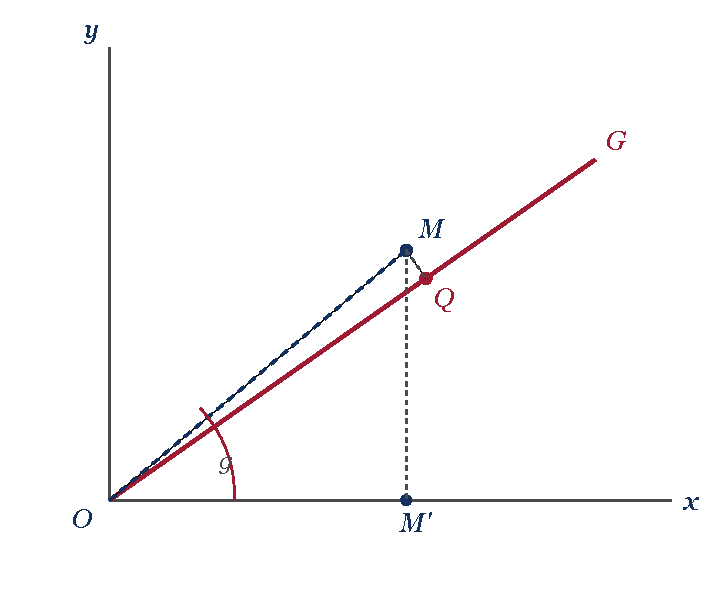
\includegraphics[width=0.55\textwidth]{figuras/pdf/cap02-fig1.pdf}
\caption{Descomposición de la vibración $OM$ en la dirección $OG$ del
polarizador $\Pi''$: $OQ$ es la componente que sobrevive, $MQ$ la que se
destruye.}
\label{fig:cap2-1}
\end{figure}

Para obtener la intensidad luminosa en un punto $P$, buscaremos el valor
medio de $OQ^2$ para un número muy grande de vibraciones. El valor medio
de esta cantidad durante una vibración es
\[
\frac{1}{2}\Bigl[A_0^2\cos^2g+B_0'^2\sin^2g
+2A_0B_0'\sin g\cos g\cos(\theta+\psi)\Bigr].
\]

Si, antes de su paso por los polarizadores $\Pi$ y $\Pi'$, la luz era
natural, $\theta$ puede tomar una infinidad de valores, y en el valor
medio de la expresión anterior el término rectángulo que contiene
$\cos(\theta+\psi)$ desaparece. En este caso no hay interferencia.

Cuando, por el contrario, la luz está polarizada rectilíneamente antes de
su paso por los polarizadores $\Pi$ y $\Pi'$, la cantidad $\theta$ es
igual a $0$ o a $\pi$. El valor del término rectángulo es, salvo el
signo,
\[
2A_0B_0'\cos g\sin g\cos\psi;
\]
su valor medio durante un gran número de vibraciones contendrá
$\cos\psi$, y los rayos interferirán.


% ============================================================
% Capítulo III — Principio de Huygens
% Traducción de "Théorie mathématique de la lumière" (1889), cap. III
% Original: §§61-75, páginas 76-98
% ============================================================
\chapter{Principio de Huygens}
\label{cap:huygens}

\noindent\textbf{61.}\footnote{El original numera también 61 este párrafo,
repitiendo el número del último párrafo del Capítulo~II. Conservamos la
numeración de Poincaré.~(N.~del T.)} El principio de Huygens, en el que se apoya la teoría
de la difracción, ha sido objeto de numerosas objeciones. Para disipar esas
objeciones y dar una justificación tan completa como sea posible de este
importante principio, nos veremos obligados a detenernos largamente en este
tema.

Expongamos primero las ideas de Huygens. Supongamos que, estando en reposo
todas las moléculas del éter, se da un ebranlement\footnote{Conservamos aquí
puntualmente el sentido físico del término francés \emph{ébranlement}: una
sacudida o perturbación inicial impartida a las moléculas del medio, origen
de la onda. En el resto del capítulo se traduce simplemente como
\emph{perturbación} o \emph{sacudida inicial}.~(N.~del T.)} —una perturbación inicial—
a las contenidas en el interior de una esfera $A$ (figura~\ref{fig:cap3-1})
de radio muy pequeño, y que luego se abandona el éter a sí mismo. La
perturbación comunicada a las moléculas de $A$ se propagará en el éter;
Huygens admite que se produce una onda esférica, y que, al cabo de un tiempo
$t$, las únicas moléculas en movimiento ocupan una capa infinitamente
delgada situada en la superficie de una esfera $S$ de radio $Vt$,
concéntrica con $A$. Esta hipótesis equivale a admitir la posibilidad de
propagación de una onda aislada y, aunque experimentalmente la realización
de este hecho nunca tenga lugar, se puede usar esta abstracción en la
teoría. Siendo así, las únicas moléculas en movimiento al cabo del tiempo
$t+t'$ estarán situadas en una capa esférica $S'$ concéntrica con $S$ y de
radio $V(t+t')$.

\begin{enunciado}{Principio de Huygens}
El movimiento del éter en todo punto de la onda $S'$ es la resultante de
los movimientos que enviarían aisladamente todos los elementos de la misma
onda, considerada en una posición anterior $S$.
\end{enunciado}

Si este principio es cierto, debe poder deducirse de él que las moléculas en
movimiento al tiempo $t+t'$ están todas situadas en el interior de la capa
$S'$. Ahora bien, la onda parcial que proviene de la propagación del
movimiento que animaba, en el tiempo $t$, a un elemento $B$ de la onda $S$,
será una esfera de centro $B$ y radio $Vt'$; esa onda $s$ es, por tanto,
tangente a la onda $S'$. Lo mismo ocurrirá para todas las ondas parciales, y
se puede considerar la onda $S'$ como la envolvente de las ondas parciales
provenientes de los distintos puntos de $S$. Resulta entonces evidente que
no podrá haber movimiento más allá de la onda $S'$. Pero nada prueba
\emph{a priori} que no lo haya más acá. A primera vista, incluso parece
difícil que así sea, pues los movimientos de las moléculas de la esfera de
perturbación, al parecer tener el mismo sentido, deberían dar origen a
movimientos del mismo sentido que no pueden destruirse. Huygens explicaba
esta anomalía admitiendo que, siendo la capa $S$ infinitamente delgada, los
movimientos provenientes de la perturbación de los distintos elementos de
esa superficie debían ser infinitamente pequeños, y que solo podían ser
apreciables en la superficie $S'$, donde se componen un gran número de esos
movimientos. Esta explicación no resiste un análisis riguroso.

\begin{figure}[ht]
\centering
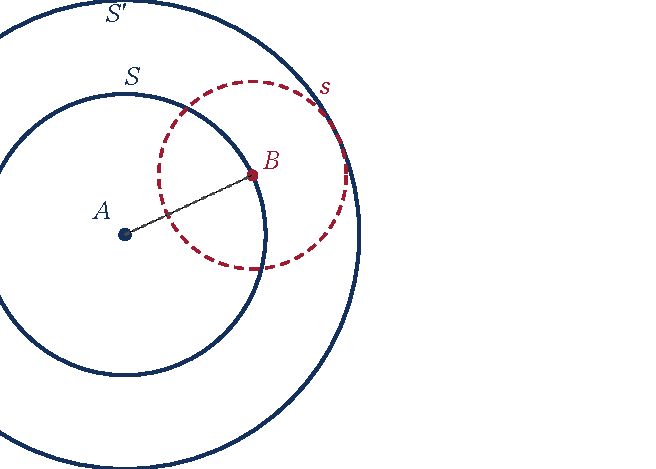
\includegraphics[width=0.85\textwidth]{figuras/pdf/cap03-fig1.pdf}
\caption{Esquema de Huygens: la perturbación inicial en la esfera $A$ se
propaga como onda esférica $S$, y luego como $S'$.}
\label{fig:cap3-1}
\end{figure}

\noindent\textbf{62.} Fresnel, en su teoría de la difracción, modifica el
principio de Huygens al considerar, ya no una onda aislada, sino una
sucesión de ondas provenientes de movimientos vibratorios. Así enuncia él
mismo este principio:

\begin{enunciado}{Principio de Huygens-Fresnel}
Las vibraciones de una onda luminosa en cada uno de sus puntos pueden
considerarse como la suma de los movimientos elementales que enviarían en
ese mismo instante, actuando aisladamente, todas las partes de esa onda
consideradas en cualquiera de sus posiciones anteriores.
\end{enunciado}

A este enunciado añade Fresnel, en nota: «Considero siempre la
sucesión de una infinidad de ondulaciones, o una vibración general del
fluido. Solo en ese sentido puede decirse que dos ondas luminosas se
destruyen cuando están a media ondulación una de otra. Las fórmulas de
interferencia que acabo de dar no son aplicables al caso de una ondulación
aislada, que por lo demás no es el de la naturaleza.»\footnote{\emph{Œuvres
de Fresnel}, t.~I, p.~293.} Al considerar así ondas sucesivas, los
movimientos de las moléculas de $S$ son unas veces en un sentido, otras en
el contrario, y puede concebirse que, al tiempo $t+t'$, las moléculas que
quedan fuera de la superficie $S'$ no estén en movimiento. Esta explicación
dista de estar libre de todo reproche, como veremos en el párrafo
siguiente. Por lo demás, la teoría de la propagación de una onda aislada
—propagación matemáticamente posible— deja subsistir una dificultad que es
necesario explicar.

\noindent\textbf{63. Controversia de Fresnel con Poisson.} — Ya se
considere una onda aislada o una serie de ondas sucesivas, el principio de
Huygens lleva a admitir que, además de la onda $S'$, se produce otra, $S''$,
que es la envolvente interior de las ondas elementales $s$. Esta es una de
las objeciones que Poisson hace a Fresnel, en una carta\footnote{\emph{Œuvres
de Fresnel}, t.~II, p.~209.} de la que extraemos el siguiente pasaje:
«También le haré notar que, en el razonamiento que lo conduce a la fórmula
de la página 287 de su Memoria sobre la difracción\footnote{Es la fórmula
$\left[\left(\int ds\cos\!\left(\pi\dfrac{s^2(a+b)}{ab\lambda}\right)\right)^2
+\left(\int ds\sin\!\left(\pi\dfrac{s^2(a+b)}{ab\lambda}\right)\right)^2\right]^{1/2}$,
que da la velocidad del desplazamiento en el punto $P$ y que Fresnel obtuvo
apoyándose en el principio de Huygens (\emph{Œuvres de Fresnel}, t.~I,
p.~316). $a$ designa la distancia $CM$, $b$ la distancia $MP$.}, nada
expresa que el punto $P$ (figura~\ref{fig:cap3-2}) esté situado más allá de
la onda $AMF$, y que, si estuviera situado más acá de esa onda, el mismo
razonamiento, aplicado palabra por palabra, lo conduciría a una fórmula
semejante para expresar la velocidad que recibe, con la única diferencia de
que, en lugar de $a+b$, esa fórmula contendría $a-b$, que sería entonces la
distancia $CP$. De sus principios se seguiría, pues, que la onda $AMF$,
incluso cuando está completa, debería producir movimiento tanto más acá como
más allá de su posición, conclusión que bastaría para mostrar que hay algún
vicio en su manera de plantear la cuestión. Y, en efecto, la producción de
una onda nueva por delante de la que usted considera, y la no comunicación
del movimiento hacia atrás, solo se dan en razón de una relación
determinada que subsiste, en la onda dada, entre las condensaciones y las
velocidades propias de las moléculas fluidas, y de ningún modo en razón de
la interferencia de las ondas elementales originadas en todos sus puntos en
instantes distintos.»

\begin{figure}[ht]
\centering
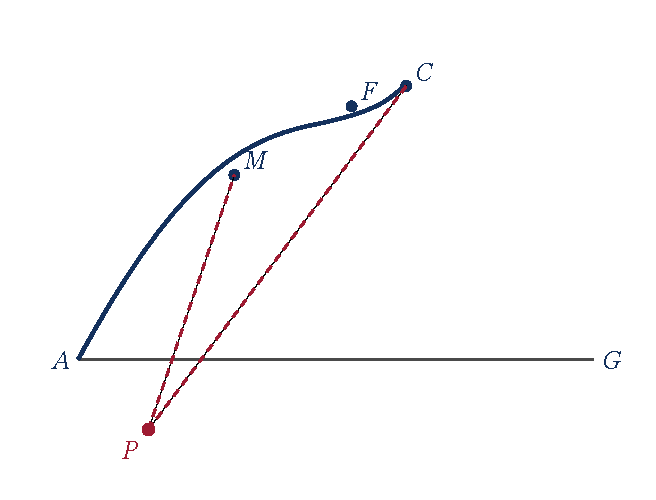
\includegraphics[width=0.85\textwidth]{figuras/pdf/cap03-fig2.pdf}
\caption{Diagrama de la carta de Poisson a Fresnel: el punto $P$ y la onda
$AMF$.}
\label{fig:cap3-2}
\end{figure}

\noindent\textbf{64.} En su respuesta a esta carta, Fresnel, tras contestar
a otras objeciones de Poisson, llega por fin a la verdadera explicación de
la anomalía que tanto tiempo había detenido a los geómetras. Hay, dice,
dos cosas que considerar en el movimiento de una molécula: la velocidad de
la que está animada y su alejamiento de su posición de equilibrio; de ahí
resultan dos sistemas de ondas derivadas.

Pero, antes de citar ese pasaje de Fresnel, debemos dar algunas
explicaciones sobre lo que él llama \emph{la ley del coseno}. En la época
de esta controversia, Fresnel ya había hecho su gran descubrimiento de la
transversalidad de las vibraciones. Pero Poisson y los geómetras de su
tiempo se negaban a admitirlo. Así, Fresnel, deseoso de reducir la
divergencia de sus puntos de vista con los de Poisson, y convencido de que
su teoría de la difracción era igualmente aplicable a todas las hipótesis,
razona constantemente como si las vibraciones fueran longitudinales.

Así llega, mediante un razonamiento que por lo demás no estaría libre de
todo reproche, a esta consecuencia: que el movimiento enviado por un punto
$B$ (figura~\ref{fig:cap3-3}) de la onda $S$ a un punto $D$ de la onda $S'$
es proporcional al coseno del ángulo $DBC$ formado por la dirección $DB$
con la normal a la onda $S$. Este razonamiento no es en absoluto aplicable
al caso de los movimientos transversales.

Por fortuna, la ley del coseno no desempeña ningún papel esencial en la
teoría de Fresnel, y debe considerarse solo como un incidente de su
controversia. Las objeciones a las que esta ley pueda dar lugar no afectan
en nada a la teoría misma.

\begin{figure}[ht]
\centering
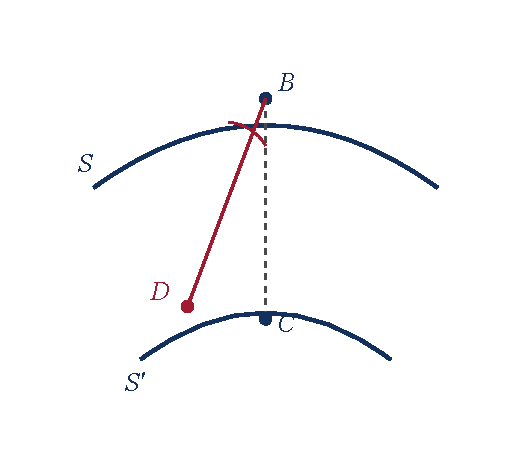
\includegraphics[width=0.7\textwidth]{figuras/pdf/cap03-fig3.pdf}
\caption{La «ley del coseno» de Fresnel: ángulo $DBC$ entre $DB$ y la
normal a la onda $S$.}
\label{fig:cap3-3}
\end{figure}

\noindent\textbf{65.} Citemos ahora el pasaje más importante de la carta de
Fresnel (\emph{Œuvres complètes}, t.~II, p.~227).

\begin{quote}
«Usted objetará quizá todavía al razonamiento que acabo de hacer para el
caso de una pequeña perturbación, que establecería la existencia de rayos
de igual intensidad en sentido opuesto, incluso cuando la perturbación
inicial formara parte de una onda derivada; pero responderé, como ya lo he
hecho, que esto no es en absoluto una consecuencia del principio en el que
me apoyo. En efecto, llego a esta ley del coseno considerando por separado
la onda producida por las velocidades impresas a las moléculas comprendidas
en el centro de perturbación, y la que resulta de sus simples
desplazamientos, para luego sumarlas: ahora bien, cuando estas dos ondas
empujan el fluido en el mismo sentido, se refuerzan mutuamente por
superposición; y si las intensidades de los distintos puntos de la
superficie siguen la ley del coseno en una y en otra, esa misma ley se dará
también en la onda resultante de su reunión. Si tienden a empujar las
moléculas del fluido en sentidos opuestos, las velocidades absolutas que
aportan se restan, y pueden incluso destruirse mutuamente, en el caso de
que sean iguales; esto es lo que ocurre con las ondas retrógradas, cuando
el centro de perturbación tiene la constitución particular de las ondas
derivadas. Considérese, por ejemplo, un elemento de una onda de este tipo
en el momento en que sus moléculas son empujadas hacia adelante, es decir,
en el sentido de propagación de la onda derivada: se sabe que entonces ese
movimiento hacia adelante va acompañado de una condensación, es decir, de
un acercamiento de las moléculas; si las moléculas estuvieran solo
desplazadas y, por lo demás, sin velocidad en ese mismo instante, de su
acercamiento resultaría una fuerza expansiva que empujaría el fluido tanto
hacia atrás como hacia adelante, y produciría así una onda retrógrada
semejante a la que excitaría hacia adelante, pero en la que las velocidades
absolutas serían de signo contrario; si, por otro lado, las moléculas se
encontraran en sus posiciones de equilibrio en el momento en que se
considera la perturbación, y recibieran solo en ese instante las
velocidades que las empujan hacia adelante, resultaría también de ello una
onda hacia atrás, igual que una onda hacia adelante, puesto que esas
moléculas serían seguidas por las que están detrás, y así sucesivamente;
la onda retrógrada tendría todavía la misma intensidad que la onda que se
propagaría hacia adelante, y desplazaría las moléculas del fluido en el
mismo sentido; pero la onda retrógrada resultante de la simple condensación
las empuja en sentido contrario. Estos dos movimientos se restarán,
entonces, el uno del otro en las ondas retrógradas debidas a la
condensación y a las velocidades de las moléculas, mientras que se sumarán
en las dos ondas que se propagan hacia adelante; si, pues, estas dos causas
tienden a producir efectos iguales, como ocurre en el caso particular de
las ondas derivadas, las ondas retrógradas se borrarán mutuamente, y las
vibraciones solo podrán propagarse en el sentido de la marcha de la onda
derivada.»
\end{quote}

Esa era, en efecto, la verdadera explicación del principio de Huygens;
vamos a mostrarla con mayor rigor en lo que sigue.

\section{Integración de las ecuaciones de los movimientos transversales en
el caso de las ondas esféricas}

\noindent\textbf{66.} Retomemos las ecuaciones de los movimientos
transversales
\[
\frac{d^2\xi}{dt^2}=V^2\Delta\xi,\qquad
\frac{d^2\eta}{dt^2}=V^2\Delta\eta,\qquad
\frac{d^2\zeta}{dt^2}=V^2\Delta\zeta,
\]
que ya resolvimos para el caso de las ondas planas (§50), y propongámonos hallar
sus integrales en el caso de las ondas esféricas.

En las ondas de esta naturaleza, los desplazamientos y las velocidades de
un punto $M$ (figura~\ref{fig:cap3-4}) deben tener los mismos valores para
todos los puntos situados a una misma distancia $r$ del centro de las
ondas; luego $\xi,\eta,\zeta$ y sus derivadas dependerán únicamente de $r$ y
del tiempo $t$. Tomando como origen de coordenadas el centro de las ondas
esféricas y llamando $x,y,z$ a las coordenadas del punto $M$, tendremos
\[
r^2=x^2+y^2+z^2.
\]
Pongamos
\[
\xi=\frac{u}{r},
\]
siendo $u$ una función cualquiera de $r$ y de $t$, y busquemos cuál debe ser
la forma de esta función para que satisfaga las ecuaciones del movimiento.

La cantidad $\Delta\xi$ es una función lineal y homogénea de $u$ y de sus
dos primeras derivadas respecto de $r$; podemos escribirla
\[
\Delta\xi = Au + B\frac{du}{dr} + C\frac{d^2u}{dr^2}.
\]

\begin{figure}[ht]
\centering
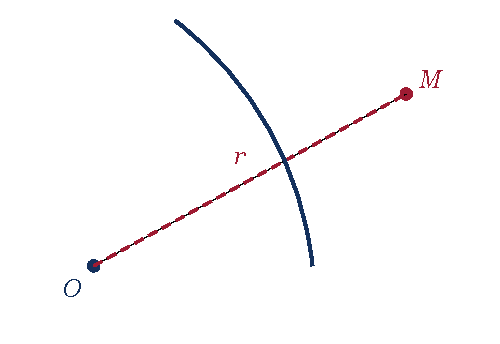
\includegraphics[width=0.85\textwidth]{figuras/pdf/cap03-fig4.pdf}
\caption{Onda esférica de centro $O$: el punto $M$ a distancia $r$.}
\label{fig:cap3-4}
\end{figure}

\noindent\textbf{67.} El valor de los coeficientes $A,B,C$ podría obtenerse
calculando las derivadas segundas de $\xi$ respecto de $x,y,z$ y
sumándolas, pero resulta más simple determinarlos haciendo hipótesis
particulares sobre la función $u$.

Supongamos primero que $u=1$; entonces $\xi=1/r$. Es la forma de la función
potencial en la atracción de dos puntos según la ley de Newton. Debe
tenerse entonces $\Delta\xi=0$, y como la expresión de $\Delta\xi$ se
reduce a $A$ en este caso particular, $A$ debe ser nulo.

Tomemos $u=r$; tendremos $\xi=1$, y por tanto $\Delta\xi=0$. Por otra
parte, tenemos $du/dr=1$, $d^2u/dr^2=0$; por consiguiente, como $A$ es nulo
según lo anterior,
\[
\Delta\xi = B\,\frac{du}{dr} = 0.
\]
El coeficiente $B$ debe ser, entonces, también nulo.

Para hallar el coeficiente $C$, hagamos $u=r^3$; la derivada segunda de
esta función respecto de $r$ será igual a $6r$, y el valor de $\Delta\xi$
se reducirá a $\Delta\xi=6Cr$. Pero si $u=r^3$, tenemos
$\xi=r^2=x^2+y^2+z^2$, y el cálculo da para $\Delta\xi$: $\Delta\xi=6$.
Igualando estos dos valores de $\Delta\xi$, obtenemos para $C$:
$C=1/r$.

La expresión de $\Delta\xi$ en el caso general es, por tanto,
\[
\Delta\xi = \frac{1}{r}\frac{d^2u}{dr^2}.
\]

Sustituyendo este valor en la primera de las ecuaciones del movimiento y
reemplazando $d^2\xi/dt^2$ por su valor $\frac{1}{r}\dfrac{d^2u}{dt^2}$,
obtendremos una ecuación que determinará $u$; esta ecuación es
\[
\frac{1}{r}\frac{d^2u}{dt^2} = V^2\frac{1}{r}\frac{d^2u}{dr^2},
\]
o bien
\[
\frac{d^2u}{dt^2} = V^2\frac{d^2u}{dr^2}.
\]
Integrando, se obtiene
\[
u = F(r-Vt) + F_1(r+Vt),
\]
de donde
\[
\xi = \frac{F(r-Vt)}{r} + \frac{F_1(r+Vt)}{r}.
\]

\noindent\textbf{68.} Siendo $F$ y $F_1$ funciones arbitrarias, podemos
suponer que una de ellas, $F_1$, se reduzca a $0$; tendremos entonces
\[
\xi = \frac{F(r-Vt)}{r},
\]
expresión que satisface las ecuaciones del movimiento. Por consiguiente, en
el caso general, $\xi$ puede considerarse como el desplazamiento resultante
de dos movimientos que se propagan por ondas esféricas a partir del centro
$O$, uno con velocidad $V$, el otro con velocidad $-V$. El factor $1/r$ que
aparece en la expresión de $\xi$ muestra que el movimiento se debilita a
medida que nos alejamos del centro de la perturbación.

Las dos últimas ecuaciones de los movimientos transversales darían, para
$\eta$ y $\zeta$, expresiones análogas a la que acabamos de hallar para
$\xi$.

\noindent\textbf{69.} Cuando se dan los valores iniciales de las
componentes de las velocidades, el movimiento queda completamente
determinado y se pueden hallar las funciones $F$ y $F_1$. Supongamos que en
el tiempo $t=0$ tenemos
\[
\xi=\varphi(r),\qquad \frac{d\xi}{dt}=\psi(r).
\]
Haciendo $t=0$ en la expresión de $\xi$, e igualando al valor dado
$\varphi(r)$, obtenemos la relación
\[
r\varphi(r) = F(r) + F_1(r). \tag{1}
\]
La derivada de $\xi$ respecto del tiempo es
\[
\frac{d\xi}{dt} = -V\frac{F'(r-Vt)}{r} + V\frac{F_1'(r+Vt)}{r};
\]
su valor para $t=0$ se reduce a
\[
\frac{d\xi}{dt} = -V\frac{F'(r)}{r} + V\frac{F_1'(r)}{r}.
\]
Tenemos, entonces, la relación
\[
r\psi(r) = V\bigl(F_1'-F'\bigr). \tag{2}
\]
Las relaciones (1) y (2) determinarán las funciones $F$ y $F_1$.

Una solución particular de las ecuaciones de los movimientos transversales
que resulta interesante en óptica es aquella en la que se tiene
\[
F_1(r)=0,\qquad F(r)=e^{-i\alpha r}.
\]
El valor de $\xi$ es entonces
\[
\xi = \frac{e^{-i\alpha(r-Vt)}}{r}.
\]
Su derivada segunda respecto de $t$ vale $-\alpha^2V^2\xi$.\footnote{El
original dice «a pour valeur $\alpha^2V^2\xi$», omitiendo el signo
menos, que sin embargo sí aparece en la línea siguiente. En efecto,
$\frac{d}{dt}e^{-i\alpha(r-Vt)}=i\alpha V\,e^{-i\alpha(r-Vt)}$, y derivando
otra vez se obtiene el factor $(i\alpha V)^2=-\alpha^2V^2$.~(N.~del T.)} Como $\xi$
satisface las ecuaciones del movimiento, debe cumplirse
\[
\frac{d^2\xi}{dt^2}=V^2\Delta\xi,\qquad
-\alpha^2V^2\xi = V^2\Delta\xi,
\]
o, finalmente,
\[
\Delta\xi + \alpha^2\xi = 0.
\]

\section{Integrales generales de las ecuaciones de los movimientos
transversales}

\noindent\textbf{70.} Consideremos la primera de estas ecuaciones, que
escribiremos en la forma
\[
\frac{d^2\xi}{dt^2}=V^2\Delta\xi. \tag{1}
\]
Tendremos la integral general de esta ecuación si encontramos una función
$\xi$ de $x,y,z$ y $t$ que la satisfaga idénticamente y que se reduzca,
para $t=0$, a una función arbitraria de $x,y,z$, mientras que su derivada
$d\xi/dt$ se reduzca también, para $t=0$, a otra función arbitraria de
$x,y,z$. La integral general contiene, pues, dos funciones arbitrarias.

Veamos primero a qué nos conduce la aplicación del principio de Huygens.
Supongamos que, en el origen de los tiempos, todas las moléculas del éter
estén perturbadas de tal modo que la perturbación inicial en el punto
$x',y',z'$ sea igual a $F(x',y',z')$. Al cabo del tiempo $t$, el punto
$x',y',z'$ habrá enviado una perturbación igual a $F/r$ a todos los puntos
$x,y,z$ situados a una distancia $r=Vt$ del punto $x',y',z'$, y no habrá
enviado ninguna a los puntos situados a una distancia mayor o menor.

Luego, según el principio de Huygens, el punto $x,y,z$ habrá recibido en el
instante $t$ una perturbación $F/r$ de todos los puntos $x',y',z'$ de la
esfera que tiene por centro $x,y,z$ y por radio $r=Vt$, y no habrá recibido
ninguna de ningún otro punto del espacio.

Pongamos, pues,
\[
\xi = \int \frac{F(x',y',z')}{r}\,d\omega, \tag{2}
\]
extendiéndose la integral a todos los elementos $d\omega$ de la esfera de
centro $x,y,z$ y radio $r=Vt$, y designando $x',y',z'$ las coordenadas del
elemento $d\omega$. El valor de la integral dependerá evidentemente del
centro y del radio de esta esfera, y por consiguiente $\xi$ será función de
$x,y,z$ y de $t$. Debemos, pues, para justificar el principio de Huygens,
demostrar que el valor (2) de $\xi$ satisface la ecuación (1).

Calculemos $d\xi/dx$. Para ello, demos a $x$ un
incremento $dx$ conservando $y$, $z$, $t$ —y por consiguiente $r$— sus
valores; esto equivale a dar a la esfera una traslación $dx$ paralela al
eje $x$. De ello resultará, para $x'$, un incremento $dx$, mientras que
$y'$, $z'$, $d\omega$ y $r$ conservarán el mismo valor. El incremento de
$F(x',y',z')$ será $\dfrac{dF}{dx'}dx$, y tendremos
\[
d\xi = \int \frac{dF}{dx'}\,\frac{dx\,d\omega}{r}.
\]
Como el incremento de $x'$ es el mismo para todos los elementos de la
integral, podemos sacar $dx$ como factor, y dividiendo ambos miembros de la
igualdad por esta cantidad, obtenemos
\[
\frac{d\xi}{dx} = \int \frac{dF}{dx'}\,\frac{d\omega}{r}.
\]
Derivando una segunda vez respecto de $x$, obtenemos, para la derivada
segunda,
\[
\frac{d^2\xi}{dx^2} = \int \frac{d^2F}{dx'^2}\,\frac{d\omega}{r}.
\]
El mismo razonamiento conduciría a las expresiones
\[
\frac{d^2\xi}{dy^2} = \int \frac{d^2F}{dy'^2}\,\frac{d\omega}{r},\qquad
\frac{d^2\xi}{dz^2} = \int \frac{d^2F}{dz'^2}\,\frac{d\omega}{r},
\]
para las derivadas segundas de $\xi$ respecto de $y$ y de $z$. Sumando
estas derivadas segundas, obtenemos
\[
\Delta\xi = \int \Delta F(x',y',z')\,\frac{d\omega}{r}. \tag{3}
\]

\noindent\textbf{71.} Busquemos ahora la derivada segunda de la integral
(2) respecto del tiempo. Si damos al tiempo $t$ un incremento $dt$ sin
variar $x,y,z$, el centro de la esfera no cambiará, pero su radio sufrirá
un incremento
\[
dr = V\,dt.
\]
El elemento de superficie $d\omega$ se convertirá en $d\omega'$. Podemos
hacer desaparecer $d\omega$ de la integral introduciendo el ángulo sólido
$d\sigma$ bajo el cual se ve este elemento desde el centro de la esfera; se
tiene
\[
d\omega = r^2\,d\sigma,\qquad\text{de donde}\qquad \frac{d\omega}{r}=r\,d\sigma.
\]
Por consiguiente, la integral se convierte en
\[
\xi = \int F(x',y',z')\,r\,d\sigma, \tag{4}
\]
y como $r$ es el mismo para todos los elementos de la integral, podemos
escribir
\[
\xi = r\int F(x',y',z')\,d\sigma.
\]

Si, pues, $r$ sufre un incremento $dr$, el incremento $d\xi$ que de ello
resultará para $\xi$ será\footnote{El original dice
«$d\xi = dr\int F\,d\sigma = r\,d.\!\int F\,d\sigma$», con un signo $=$ en
lugar de $+$: es una errata evidente, pues se trata simplemente de la regla
del producto aplicada a $r\cdot\int F\,d\sigma$, como confirma la línea
siguiente.~(N.~del T.)}
\[
d\xi = dr\int F\,d\sigma + r\,d\!\int F\,d\sigma,
\]
o bien
\[
d\xi = dr\int F\,d\sigma + r\,dr\int \frac{dF}{dr}\,d\sigma.
\]

Para calcular el valor de la segunda integral que entra en esta expresión,
observemos que, siendo el radio $r$ normal al elemento de superficie
$d\omega$, la derivada $dF/dr$ no es otra cosa que la derivada normal de
$F$: si se describe cada punto de la esfera por un vector unitario
$\mathbf{n}=(n_1,n_2,n_3)$, de modo que $(x',y',z')=(x+rn_1,\,y+rn_2,\,z+rn_3)$,
la regla de la cadena da
$dF/dr = \frac{dF}{dx'}n_1+\frac{dF}{dy'}n_2+\frac{dF}{dz'}n_3=\nabla F\cdot\mathbf{n}$,
y $\mathbf{n}$ es precisamente la normal exterior a la esfera en ese punto.
Se tiene, pues, según el teorema de Green —el teorema de la divergencia,
$\int_B \nabla\!\cdot\!\mathbf{G}\,d\tau=\int_S \mathbf{G}\cdot\mathbf{n}\,d\omega$,
aplicado al campo $\mathbf{G}=\nabla F$, cuya divergencia es $\Delta F$—,
\[
\int \frac{dF}{dr}\,d\omega = \int \Delta F\,d\tau,
\]
siendo $d\tau$ un elemento de volumen, y extendiéndose la integral del
segundo miembro a toda la esfera. Introduciendo en esta última igualdad el
ángulo sólido $d\sigma$ que corresponde a $d\omega$, y recordando que
$d\omega=r^2d\sigma$, se convierte en
\[
\int \frac{dF}{dr}\,d\sigma = \frac{1}{r^2}\int \Delta F\,d\tau. \tag{5}
\]

Podemos, pues, reemplazar el valor hallado antes para $d\xi$ por el
siguiente:
\[
d\xi = dr\int F\,d\sigma + \frac{dr}{r}\int \Delta F\,d\tau;
\]
o, dividiendo por $dr=V\,dt$,
\[
\frac{1}{V}\frac{d\xi}{dt} = \int F\,d\sigma + \frac{1}{r}\int \Delta F\,d\tau. \tag{6}
\]
Diferenciando esta última expresión respecto de $r$, obtenemos la igualdad
\[
\frac{1}{V^2}\frac{d^2\xi}{dt^2} = \int \frac{dF}{dr}\,d\sigma -
\frac{1}{r^2}\int \Delta F\,d\tau + \frac{1}{r}\frac{d}{dr}\cdot\int \Delta F\,d\tau,
\]
que, teniendo en cuenta la relación (5), se reduce a
\[
\frac{1}{V^2}\frac{d^2\xi}{dt^2} = \frac{1}{r}\frac{d}{dr}\cdot\int \Delta F\,d\tau. \tag{7}
\]

El segundo miembro de esta relación es, salvo el factor $\dfrac{1}{r\,dr}$,
el valor de la integral $\int \Delta F\,d\tau$ extendida a los elementos de
volumen de una capa comprendida entre las esferas de radios $r$ y $r+dr$.
Consideremos uno de estos elementos, limitado por esas dos esferas y por un
cono que tiene por vértice el centro común de ambas esferas y por base el
elemento $d\omega$ de la superficie de la primera esfera. El volumen de
este elemento se obtiene integrando en la dirección radial el área
$\rho^2\,d\sigma$ de la sección a distancia $\rho$ del centro:
\begin{align*}
\int_r^{r+dr}\rho^2\,d\sigma\,d\rho
&= \frac{(r+dr)^3-r^3}{3}\,d\sigma
= \bigl(r^2\,dr + r\,dr^2 + \tfrac13\,dr^3\bigr)\,d\sigma \\
&= d\omega\,dr + \Bigl(\frac{dr}{r}+\frac{dr^2}{3r^2}\Bigr)\,d\omega\,dr .
\end{align*}
Contando $d\omega$ como infinitésimo de segundo orden y $dr$ como de primer
orden, $d\omega\,dr$ es de tercer orden, y los demás términos son de
cuarto orden o superior; del mismo modo, dentro de este elemento $\Delta F$
difiere de su valor en la base solo en una cantidad de orden $dr$, lo que
produce igualmente términos de cuarto orden. Despreciando todo ello, el
volumen del elemento será, pues, $d\omega\,dr$. Por consiguiente, la
integral anterior se convierte en
\[
\int \Delta F\,d\omega\,dr,\qquad\text{o bien}\qquad dr\int \Delta F\,d\omega,
\]
integral extendida a todos los elementos de la esfera de radio $r$. Se
obtiene entonces, para la relación (7),
\[
\frac{1}{V^2}\frac{d^2\xi}{dt^2} = \frac{1}{r}\int \Delta F\,d\omega. \tag{8}
\]

\noindent\textbf{72.} Sustituyendo, en la ecuación (1) del movimiento,
$d^2\xi/dt^2$ por su valor tomado de esta última relación, y $\Delta\xi$
por su valor (3), la ecuación quedará satisfecha. Por consiguiente,
\[
\xi = \int \frac{F(x',y',z')}{r}\,d\omega
\]
es una solución particular de la ecuación del movimiento. Aún no puede ser
la integral general, pues solo contiene una función arbitraria.

Busquemos los valores iniciales de $\xi$ y de $d\xi/dt$. Cuando $t$ tiende
a cero, el radio de la esfera $r$ tiende a cero, y el valor de
$F(x',y',z')$ tiende a $F(x,y,z)$. Si $x',y',z'$ difieren poco de $x,y,z$,
la integral $\int F(x',y',z')\,d\sigma$ tendrá un valor próximo a
\[
F(x,y,z)\int d\sigma = 4\pi F(x,y,z).
\]
De ello resulta que el valor de $\xi$ dado por la expresión (4) difiere
poco de $r\cdot 4\pi F(x,y,z)$. En el límite, cuando $r$ es igual a cero,
$\xi$ es, por tanto, nulo. En consecuencia, el valor inicial de $\xi$ es
nulo.

La relación (6) nos da, para $d\xi/dt$,
\[
\frac{d\xi}{dt} = V\int F\,d\sigma + \frac{V}{r}\int \Delta F\,d\tau.
\]
El segundo término del segundo miembro puede despreciarse cuando el radio
$r$ es infinitamente pequeño. En efecto, la integral que contiene, al
extenderse a todos los elementos de la esfera, será un infinitésimo de
tercer orden; su cociente por $r$ será de segundo orden y será despreciable
frente al primer término, cuyo valor en el límite es $4\pi V F$. Tendremos,
pues,
\[
\left(\frac{d\xi}{dt}\right)_0 = 4\pi V F(x,y,z). \tag{9}
\]
Como la función $F$ es arbitraria, la velocidad inicial del desplazamiento
es arbitraria.

\noindent\textbf{73.} Para obtener la integral general de la ecuación del
movimiento, necesitamos hallar una segunda solución particular cuyo valor
inicial pueda tomarse arbitrariamente. Vamos a mostrar que
\[
\xi' = \frac{1}{V}\frac{d\xi}{dt}
\]
satisface estas condiciones.

En primer lugar, es una solución de la ecuación del movimiento. En efecto,
se tiene
\[
\frac{d^2\xi'}{dt^2} = \frac{1}{V}\frac{d^3\xi}{dt^3}
= \frac{1}{V}\frac{d}{dt}\cdot\frac{d^2\xi}{dt^2},
\]
y
\[
\Delta\xi' = \frac{d^2}{dx^2}\cdot\frac{1}{V}\frac{d\xi}{dt}
+ \frac{d^2}{dy^2}\cdot\frac{1}{V}\frac{d\xi}{dt}
+ \frac{d^2}{dz^2}\cdot\frac{1}{V}\frac{d\xi}{dt}
= \frac{1}{V}\frac{d}{dt}\cdot\Delta\xi.
\]
Por consiguiente, para que la ecuación del movimiento quede satisfecha, es
necesario que se tenga
\[
\frac{1}{V}\frac{d}{dt}\cdot\frac{d^2\xi}{dt^2} = V^2\cdot\frac{1}{V}\frac{d}{dt}\Delta\xi,
\]
o bien
\[
\frac{d}{dt}\cdot\frac{d^2\xi}{dt^2} = V^2\frac{d}{dt}\Delta\xi.
\]
Esta igualdad queda satisfecha pues se obtiene diferenciando respecto de
$t$ la ecuación (1), a la cual $\xi$ satisface idénticamente.

Para obtener el valor inicial de $\xi'$ basta buscar en qué se convierte la
relación (6) cuando en ella se hace $t=0$. Según lo dicho antes en la
búsqueda del valor inicial de $d\xi/dt$, se tendrá
\[
(\xi')_0 = 4\pi F(x,y,z). \tag{10}
\]
Se puede, pues, tomar un valor cualquiera para el valor inicial del
desplazamiento, puesto que la función $F$ es arbitraria.

El valor inicial de $d\xi'/dt$ se deduce de la relación (8). Se tiene
\[
\frac{d\xi'}{dt} = \frac{1}{V}\frac{d^2\xi}{dt^2} = \frac{V}{r}\int \Delta F\,d\omega;
\]
por consiguiente, el valor inicial de la velocidad $d\xi'/dt$ es nulo.

\noindent\textbf{74.} La suma de las dos soluciones particulares $\xi$ y
$\xi'$ que acabamos de hallar será la solución más general de la ecuación
del movimiento. Esta solución es
\[
\xi = \int \frac{F(x',y',z')}{r}\,d\omega + \int F_1(x',y',z')\,d\sigma
+ \frac{1}{r}\int \Delta F_1\,d\tau,
\]
designando por $F_1$ la función arbitraria que entra en la segunda solución
particular.

Busquemos la expresión de esta solución cuando se dan los valores iniciales
del desplazamiento y de la velocidad:
\[
\xi_0=\varphi(x,y,z),\qquad \left(\frac{d\xi}{dt}\right)_0=\psi(x,y,z).
\]
El valor inicial de la expresión general de $\xi$ se reduce al valor
inicial de la segunda solución particular; por consiguiente, la relación
(10) nos da
\[
\varphi = 4\pi F_1.
\]
Siendo nula la velocidad inicial de la segunda solución particular,
tendremos, según la relación (9),
\[
\psi = 4\pi V F.
\]
Sustituyendo, en la expresión general de $\xi$, las funciones $F$ y $F_1$
por sus valores tomados de estas últimas relaciones, obtenemos
\[
\xi = \int \frac{\psi\,d\omega}{4\pi Vr} + \int \frac{\varphi\,d\sigma}{4\pi}
+ \frac{1}{r}\int \frac{\Delta\varphi\cdot d\tau}{4\pi},
\]
o bien, la solución general de la ecuación del movimiento en términos del
desplazamiento inicial $\varphi$ y de la velocidad inicial $\psi$:

\begin{enunciado}{Solución general de la ecuación del movimiento}
\begin{equation}
\xi = \frac{1}{4\pi}\int \frac{d\omega}{r}
\left(\frac{\psi}{V} + \frac{\varphi}{r} + \frac{d\varphi}{dr}\right).
\tag{11}
\end{equation}
\end{enunciado}

\section{Justificación del principio de Huygens}

\noindent\textbf{75.} La expresión anterior muestra que el valor, en el
tiempo $t$, del desplazamiento de un punto de una esfera de radio $Vt$
depende a la vez de los valores del desplazamiento y de la velocidad del
centro de la esfera en el origen de los tiempos. De ahí vamos a extraer la
justificación del principio de Huygens, ya sea en el caso de una onda
aislada, ya sea en el de una serie de ondas periódicas.

Supongamos, como hacía Huygens, que se perturban las moléculas de una
esfera de radio infinitamente pequeño. Esta perturbación se propagará por
ondas esféricas, y en cierto momento las moléculas perturbadas estarán
situadas en una capa $S$ comprendida entre dos esferas de radios $r_0$ y
$r_0+\varepsilon$. El desplazamiento de una molécula vendrá dado por la
fórmula
\[
\xi = \frac{F(r-Vt)}{r},
\]
que hallamos (§68) para el caso de la propagación por ondas esféricas. Como
solo hay movimiento en la capa esférica, $\xi$ —y por tanto $F$— deberán
ser nulos en todo punto situado fuera de esta capa. Esta función $F$, nula
en $r_0$ y en $r_0+\varepsilon$, debe pasar por un máximo o un mínimo para
algún valor de $r$ comprendido entre $r_0$ y $r_0+\varepsilon$; por
consiguiente, su derivada respecto de $r$ no tiene el mismo signo en todos
los puntos de la capa. Ahora bien, la velocidad de una molécula vale
\[
\frac{d\xi}{dt} = -\frac{V}{r}F'_r;
\]
debe, pues, cambiar de signo para algún valor de $r$ tal que
$r_0<r<r_0+\varepsilon$.

Al cabo del tiempo $t+t'$, solo habrá movimiento en el interior de una capa
esférica $S'$ limitada por dos esferas concéntricas de radios $r_0+Vt'$ y
$r_0+\varepsilon+Vt'$. Por otra parte, si queremos obtener el valor de
$\xi$ en el instante $t+t'$ y en un punto $P$ cualquiera del espacio,
podemos considerar las distintas moléculas de $S$ como centros de
perturbación. Ese valor de $\xi$ nos vendrá dado por la fórmula (11) del
§74:
\[
\xi = \frac{1}{4\pi}\int \frac{d\omega}{r'}
\left(\frac{\psi}{V} + \frac{\varphi}{r'} + \frac{d\varphi}{dr'}\right).
\]
La integral debe extenderse a todos los elementos $d\omega$ de una esfera
de centro $P$ y radio $r'=Vt'$, o más bien a todos aquellos de estos
elementos que pertenecen a la capa infinitamente delgada $S$; $\varphi$
designa el valor del desplazamiento del centro de gravedad de $d\omega$ en
el instante $t$, y $\psi$ representa el valor de la velocidad de ese mismo
punto en ese mismo instante.

Se trata de explicar cómo la expresión de $\xi$ así obtenida es nula cada
vez que el punto $P$ no pertenece a la capa $S'$. Esto se comprende
observando que la velocidad inicial $\psi$ no conserva siempre el mismo
signo, como acabamos de ver. La integral tiene, pues, elementos positivos y
negativos, y se concibe que pueda ser nula.

Nos bastará con haber mostrado que no hay aquí ninguna anomalía real; el
cálculo mostraría que la integral se anula efectivamente para todos los
puntos del espacio situados fuera de $S'$.

\begin{notahistorica}
La controversia entre Fresnel y Poisson sobre el principio de Huygens es
uno de los episodios más conocidos de la óptica del siglo~\textsc{xix}.
Poisson, defensor de la teoría corpuscular de la luz, buscaba mostrar
contradicciones internas en la naciente teoría ondulatoria de Fresnel; su
objeción llevó, indirectamente, a que Arago verificara experimentalmente la
predicción —hoy célebre como «punto de Poisson» o «punto de Arago»— de
una mancha luminosa en el centro de la sombra de un disco opaco, una de las
confirmaciones más contundentes de la naturaleza ondulatoria de la luz.
\end{notahistorica}


% ============================================================
% Capítulo IV — Difracción (§§76-120)
% Traducción de "Théorie mathématique de la lumière" (1889), cap. IV
% Original: §§76-120, páginas impresas 99-175
% Teoría general §§76-99; casos aplicados §§100-120.
% ============================================================
\chapter{Difracción}
\label{cap:difraccion}

\section{Ecuaciones de los movimientos transversales en el caso de
desplazamientos periódicos}

\noindent\textbf{76. Ecuaciones de los movimientos transversales en el
caso de desplazamientos periódicos.} — Supongamos que las componentes
$\xi,\eta,\zeta$ del desplazamiento sean funciones periódicas del tiempo;
el valor de la componente $\xi$ puede entonces escribirse
\[
\xi = A\cos\frac{2\pi Vt}{\lambda} + B\sin\frac{2\pi Vt}{\lambda}
\]
siendo $A$ y $B$ funciones de $x,y,z$ solamente. Observando que $\cos x$
es la parte real de la exponencial $e^{-ix}$ y $\sin x$ la parte real de
$-ie^{-ix}$, se puede considerar $\xi$ como la parte real de la
exponencial
\[
(A-Bi)\,e^{-\frac{2i\pi Vt}{\lambda}},
\]
o bien
\[
\xi_0\,e^{-\frac{2i\pi Vt}{\lambda}}.
\]
Ahora bien, siendo lineales las ecuaciones de los movimientos
transversales respecto de las derivadas segundas de $\xi,\eta,\zeta$, si
una exponencial de esta forma satisface esas ecuaciones, la parte real y
la parte imaginaria las satisfarán por separado. Podremos, pues, como ya
dijimos (§51), buscar las soluciones de la forma
\[
\xi = \xi_0\,e^{-i\alpha Vt}
\]
y tomar después, como valor de la componente del desplazamiento, la parte
real de esta solución, habiendo puesto, para simplificar, $2\pi/\lambda=\alpha$.

La derivada segunda de $\xi$ respecto de $t$ será
\[
\frac{d^2\xi}{dt^2} = -\alpha^2V^2\xi_0\,e^{-i\alpha Vt},
\]
no dependiendo $\xi_0$ del tiempo, puesto que las funciones $A$ y $B$ no
dependen de él. La derivada segunda respecto de $x$ es
$d^2\xi/dx^2 = (d^2\xi_0/dx^2)\,e^{-i\alpha Vt}$; por consiguiente se
tendrá $\Delta\xi = \Delta\xi_0\,e^{-i\alpha Vt}$.

Para que la primera ecuación de los movimientos transversales,
$d^2\xi/dt^2=V^2\Delta\xi$, quede satisfecha, es necesario, pues, que se
tenga $-\alpha^2V^2\xi_0 e^{-i\alpha Vt} = V^2\Delta\xi_0 e^{-i\alpha Vt}$,
es decir,
\begin{equation}
\Delta\xi_0+\alpha^2\xi_0=0.
\tag{1}
\end{equation}
Las otras dos ecuaciones del movimiento nos darían dos nuevas ecuaciones
de condición,
\begin{equation}
\Delta\eta_0+\alpha^2\eta_0=0,
\tag{2}
\end{equation}
\begin{equation}
\Delta\zeta_0+\alpha^2\zeta_0=0.
\tag{3}
\end{equation}
Además, siendo transversales los movimientos, debemos tener
$\Theta=d\xi/dx+d\eta/dy+d\zeta/dz=0$; y como
$d\xi/dx=(d\xi_0/dx)e^{-i\alpha Vt}$,
$d\eta/dy=(d\eta_0/dy)e^{-i\alpha Vt}$,
$d\zeta/dz=(d\zeta_0/dz)e^{-i\alpha Vt}$, la condición de transversalidad
se convierte en
\begin{equation}
\frac{d\xi_0}{dx}+\frac{d\eta_0}{dy}+\frac{d\zeta_0}{dz}=0.
\tag{4}
\end{equation}
Tales son las cuatro condiciones que deben cumplir $\xi_0,\eta_0,\zeta_0$
para que $\xi,\eta,\zeta$ satisfagan las ecuaciones de los movimientos
transversales.

\section{Integración de la primera de las ecuaciones de condición}

\noindent\textbf{77. Integración de la primera de las ecuaciones de
condición.} — En la búsqueda de las integrales de las ecuaciones de los
movimientos transversales en el caso de las ondas esféricas, hallamos
(§69), como solución particular de la ecuación $\Delta\xi+\alpha^2\xi=0$,
la expresión $\xi=e^{-i\alpha(r-Vt)}/r$. Por consiguiente,
$\xi_0=(1/r)e^{i\alpha r}$ será una solución particular de la ecuación
de condición (1), siendo $r$ la distancia del punto $x,y,z$ al
origen. Esta cantidad seguirá siendo solución de la misma ecuación cuando
$r$ designe la distancia del punto $x,y,z$ a un punto fijo cualquiera,
pues la ecuación diferencial conserva la misma forma al tomar por origen
el punto fijo.

Sean ahora $P_1,P_2,P_3,\dots,P_n$ cierto número de puntos fijos cuyas
distancias al punto $M$ de coordenadas $x,y,z$ son $r_1,r_2,r_3,\dots,r_n$;
la suma
\[
\xi_0 = m_1\frac{e^{i\alpha r_1}}{r_1} + m_2\frac{e^{i\alpha r_2}}{r_2} +
m_3\frac{e^{i\alpha r_3}}{r_3} + \dots + m_n\frac{e^{i\alpha r_n}}{r_n}
\]
satisfará la ecuación (1). Si se supusiera $\alpha=0$, $\xi_0$ se
reduciría a una suma de términos tales como $m_1/r_1$, es decir, que
$\xi_0$ sería el potencial en el punto $M$, supuesto atraído según la ley
de Newton por los puntos $P_1,P_2,\dots,P_n$, de masas $m_1,m_2,\dots,m_n$.
Esta analogía nos va a permitir hallar fácilmente varias soluciones
particulares de la ecuación (1).

Consideremos, en efecto, una materia atrayente repartida de manera
cualquiera en el espacio, pero de modo que la atracción, en lugar de regirse
por la ley de Newton, esté representada por la función
$\dfrac{d}{dr}\!\left(\dfrac{e^{i\alpha r}}{r}\right)$, designando $r$ la
distancia del punto atraído al punto atrayente. Según lo anterior, el
potencial debido a la atracción de esta materia satisfará la ecuación (1).

\noindent\textbf{78.} En la teoría del potencial se considera no solo la
atracción de puntos aislados, sino también la atracción de volúmenes y de
superficies. Suponiendo que los puntos $P_1,P_2,\dots,P_n$ formen un
volumen, tendremos para $\xi_0$
\begin{equation}
\xi_0 = \int \frac{e^{i\alpha r}X\,d\tau}{r}.
\tag{5}
\end{equation}
La integral se extiende a todos los elementos $d\tau$ del volumen
atrayente, y $X$ es una función cualquiera de las coordenadas del elemento
$d\tau$. Esta función $X$ representa la densidad de la materia atrayente.

Es claro que, para todo punto tomado fuera del volumen atrayente, $\xi_0$
satisfará la ecuación (1). La analogía con la teoría ordinaria del
potencial basta para advertirnos que no ocurrirá lo mismo para un punto
perteneciente al volumen atrayente. Demostremos que en un punto $P$ de ese
volumen se tendrá:
\begin{equation}
\Delta\xi_0+\alpha^2\xi_0+4\pi X=0,
\tag{6}
\end{equation}
designando aquí $X$ el valor que toma en el punto $P$ la densidad de la
materia atrayente. Es fácil reconocer que, si se hace $\alpha=0$, se cae
de nuevo en la ecuación de Poisson.

Para demostrar esta ecuación, describamos desde el punto $P$ como centro
una esfera muy pequeña $s$, y descompongamos el volumen atrayente en dos
volúmenes parciales, a saber, la esfera $s$ y el volumen $T$ situado fuera
de esa esfera. Pongamos luego
\[
\xi_0=\xi_1+\xi_2+\xi_3,
\]
donde
\begin{gather*}
\xi_1=\int X\frac{e^{i\alpha r}}{r}\,d\tau\ \text{(integral extendida al
volumen $T$)},\\
\xi_2=\int \frac{X}{r}\,d\tau\ \text{(integral extendida a $s$)},\\
\xi_3=\int X\left(\frac{e^{i\alpha r}-1}{r}\right)d\tau\ \text{(integral
extendida a $s$)}.
\end{gather*}
Estando el punto $P$ fuera del volumen $T$, se tendrá
$\Delta\xi_1+\alpha^2\xi_1=0$. Por otra parte, la ecuación de Poisson nos
da $\Delta\xi_2+4\pi X=0$. Siendo muy pequeño el radio de la esfera $s$,
tendremos, salvo infinitésimos: $\xi_2=\xi_3=0$, $\xi_1=\xi_0$.

Por otro lado, si consideramos la integral que define la función $\xi_3$,
vemos que la función bajo el signo $\int$ no se vuelve infinita para
$r=0$; concluiremos de ello que $\Delta\xi_3$ es del mismo orden de
magnitud que la esfera $s$; se tiene, pues, $\Delta\xi_3=0$,
$\Delta\xi_0=\Delta\xi_1+\Delta\xi_2$, de donde
$\Delta\xi_0+\alpha^2\xi_0+4\pi X=0$.

\noindent\textbf{79.} Consideremos ahora una superficie atrayente. El
potencial debido a la atracción de esta superficie estará representado
por la integral
\begin{equation}
\xi_0 = \int X\frac{e^{i\alpha r}}{r}\,d\omega,
\tag{7}
\end{equation}
extendida a todos los elementos $d\omega$ de la superficie atrayente; $X$
designa una función cualquiera de las coordenadas del elemento $d\omega$,
y $r$ es la distancia de ese elemento al punto atraído $x,y,z$.

Hallaremos aquí también la mayor analogía con la teoría del potencial
newtoniano, pues, si ponemos
\[
\xi_0=\xi_1+\xi_2,\qquad
\xi_1=\int \frac{X}{r}\,d\omega,\qquad
\xi_2=\int X\,\frac{e^{i\alpha r}-1}{r}\,d\omega,
\]
la primera integral es el potencial ordinario; la segunda es tal que la
función bajo el signo $\int$ no se vuelve nunca infinita; es, pues, una
función continua, así como todas sus derivadas.

Según la teoría del potencial newtoniano, $\xi_1$ es también una función
continua; luego lo es también $\xi_0$. Pero no ocurre lo mismo con sus
derivadas.

En efecto, $d\xi_0/dx$, $d\xi_0/dy$, $d\xi_0/dz$ son las componentes de la
fuerza atractiva según los tres ejes; designaremos igualmente, según el
uso, mediante la notación $d\xi_0/dn$, la proyección de esa misma fuerza
sobre la normal al elemento $d\omega$. Tendremos, pues,
\[
\frac{d\xi_0}{dn} = l\frac{d\xi_0}{dx}+m\frac{d\xi_0}{dy}+n\frac{d\xi_0}{dz},
\]
designando $l,m,n$ los cosenos directores de esa normal.

Sabemos que $d\xi_1/dn$ es una función discontinua, y que, si se consideran
dos puntos infinitamente vecinos situados a uno y otro lado del elemento
$d\omega$, los valores de esta función en esos dos puntos diferirán en
una cantidad igual a $4\pi X$. Ahora bien, $d\xi_2/dn$ es continua.
Luego $d\xi_0/dn=d\xi_1/dn+d\xi_2/dn$ será discontinua y sufrirá un salto
brusco igual a $4\pi X$ al atravesar la superficie atrayente.

\noindent\textbf{80.} Nos queda por extender al caso que nos ocupa la
teoría de la doble capa atrayente, cuyo papel es tan grande en el estudio
del potencial newtoniano.

Consideremos dos superficies paralelas infinitamente vecinas, tales que
las normales a las dos superficies sean las mismas, y que la distancia
infinitamente pequeña de esas dos superficies, contada sobre una de las
normales comunes, sea constante.

Imaginemos que se reparte materia atrayente sobre esas dos superficies, de
tal modo que las densidades en dos elementos correspondientes de las dos
superficies sean iguales y de signo contrario.

Al considerar el potencial debido a la atracción de una doble capa de este
tipo, vamos a hallar nuevas soluciones particulares de la ecuación (1).

Designemos por $\varepsilon$ la distancia que separa las dos capas, por
$X_1$ y $-X_1$ los valores de la densidad en los centros de gravedad $P$ y
$P'$ (figura~\ref{fig:cap4-1}) de dos elementos correspondientes $d\omega$,
y pongamos $F(r)=e^{i\alpha r}/r$. Tendremos, para el potencial debido a
la atracción de estos dos elementos sobre un punto $M$ situado fuera de la
capa, y cuya distancia a uno de los elementos de superficie es $r$,
\begin{equation}
X_1\,d\omega\,F(r) - X_1\,d\omega\,F(r+dr) = -X_1\,d\omega\,dr\,F'(r).
\tag{8}
\end{equation}
Para hallar el valor de $dr$ bajaremos desde el centro $P$ de uno de los
elementos una perpendicular $PQ$ sobre la recta $MP'$; la distancia $P'Q$
será, salvo un infinitésimo de segundo orden, igual a $dr$; tendremos,
pues, $dr=\varepsilon\cos\psi$, designando $\psi$ el ángulo de la recta
$MP'$ con la recta $PP'$, que es normal a cada una de las capas. Llevando
este valor a (8) obtenemos, para el potencial total,
\begin{equation}
\xi_0 = \int X_1\,\varepsilon\,d\omega\,\cos\psi\,F'(r).
\tag{9}
\end{equation}

\begin{figure}[htbp]
\centering
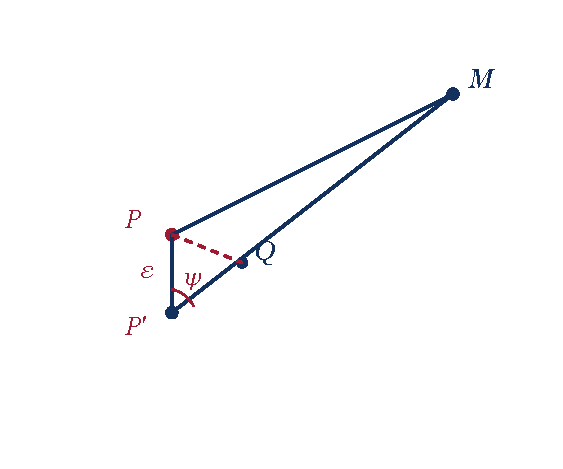
\includegraphics[width=0.55\textwidth]{figuras/pdf/cap04-fig1.pdf}
\caption{Potencial de la doble capa: los elementos correspondientes $P$ y
$P'$, de densidades $X_1$ y $-X_1$, separados por $\varepsilon$; el punto
$M$ y el ángulo $\psi$.}
\label{fig:cap4-1}
\end{figure}

Siendo arbitraria la función $X_1$, podremos, sin disminuir la generalidad
de la solución particular (9), reemplazar $X_1\varepsilon$ por una sola
letra $X_2$ que designe una función cualquiera de $x,y,z$. Además, puesto
que hemos puesto $F(r)=e^{i\alpha r}/r$, tendremos, para la derivada,
$F'(r)=\dfrac{e^{i\alpha r}}{r}\left(i\alpha-\dfrac1r\right)$. Por
consiguiente, la expresión (9) de $\xi_0$ puede escribirse
\begin{equation}
\xi_0 = \int X_2\,\frac{e^{i\alpha r}}{r}\left(i\alpha-\frac1r\right)
\cos\psi\,d\omega.
\tag{10}
\end{equation}
Pongamos aún: $\xi_0=\xi_1+\xi_2$,
\[
\xi_1 = -\int \frac{X_2\cos\psi}{r^2}\,d\omega,\qquad
\xi_2 = \int X_2\cos\psi\left[\frac{i\alpha e^{i\alpha r}}{r} -
\frac{e^{i\alpha r}}{r^2} + \frac{1}{r^2}\right]d\omega.
\]
Vemos que $\xi_1$ representa el potencial newtoniano de una doble capa. En
cuanto a la segunda integral $\xi_2$ (como la función bajo el signo $\int$
no se vuelve infinita), será continua, así como todas sus derivadas.

La teoría del potencial newtoniano nos enseña que $d\xi_1/dn$ es continua,
pero que $\xi_1$ es una función discontinua. Luego $d\xi_0/dn$ es continua
y $\xi_0$ será una función discontinua, que sufrirá un salto brusco igual
a $4\pi X_2$ al atravesar la superficie atrayente.

\noindent\textbf{81.} La combinación de las integrales (7) y (10) nos da
la solución más general de la ecuación (1).

En efecto, si $X_1$ y $X_2$ son dos funciones cualesquiera de las
coordenadas de un elemento $d\omega$ de una superficie cualquiera; si $r$
es la longitud de la recta que une el elemento $d\omega$ con el punto
$x,y,z$; y si $\psi$ designa el ángulo que forma esa recta con la normal
al elemento $d\omega$, la expresión
\begin{equation}
\xi_0 = \int X_1\frac{e^{i\alpha r}}{r}\,d\omega +
\int X_2\cos\psi\,\frac{e^{i\alpha r}}{r}\left(i\alpha-\frac1r\right)d\omega
\tag{11}
\end{equation}
satisfará la ecuación (1). Nos queda por mostrar que esa es, en efecto, la
integral general.

Sea $U$ una función cualquiera, finita y continua, así como todas sus
derivadas, y que satisface la ecuación (1) fuera de una cierta superficie
$S$.

Sea $V$ el potencial debido a un cierto volumen atrayente, cuya parte
podrá encontrarse fuera de la superficie $S$. Tendremos
\begin{equation}
\Delta V+\alpha^2V=0,
\tag{12}
\end{equation}
fuera del volumen atrayente, y en un punto de ese volumen
\begin{equation}
\Delta V+\alpha^2V+4\pi\rho=0,
\tag{13}
\end{equation}
siendo $\rho$ la densidad de la materia atrayente.

El teorema de Green nos da:
\begin{equation}
\int\left(U\frac{dV}{dn}-V\frac{dU}{dn}\right)d\omega =
\int(U\Delta V-V\Delta U)\,d\tau,
\tag{14}
\end{equation}
extendiéndose la primera integral a todos los elementos $d\omega$ de la
superficie $S$ y la segunda a todos los elementos de volumen $d\tau$ del
espacio exterior a esa superficie. En el cálculo de las derivadas
$dU/dn$ y $dV/dn$ se considera la normal al elemento $d\omega$ dirigida
hacia el interior de la superficie $S$.

Como $U$ satisface la ecuación (1) y $V$ las ecuaciones (12) y (13), la
integral del segundo miembro de (14) se reducirá a
\[
-4\pi\int U\rho\,d\tau,
\]
debiendo extenderse la integración al volumen atrayente que engendra el
potencial $V$, o más bien a la porción de ese volumen exterior a $S$.

Supongamos ahora que el volumen atrayente que engendra $V$ se reduzca a
una esfera de radio muy pequeño cuyo centro sea el punto $x_0,y_0,z_0$, y
que la densidad $\rho$ sea tal que la masa atrayente total sea igual a
$1$. Entonces, llamando $r_0$ a la distancia de un elemento $d\omega$ de
$S$ al punto $x_0,y_0,z_0$, el valor de $V$ en el centro de gravedad de
ese elemento se reducirá a $e^{i\alpha r_0}/r_0$ y el de $dV/dn$ a
$+\cos\psi\,\dfrac{e^{i\alpha r_0}}{r_0}\left(i\alpha-\dfrac{1}{r_0}\right)$,
designando siempre $\psi$ el ángulo de la normal exterior al elemento
$d\omega$ con la recta que une ese elemento con el punto $x_0,y_0,z_0$.

La integral $\int U\rho\,d\tau$ se reducirá a $U_0$ ($U_0$ el valor de $U$
en el punto $x_0,y_0,z_0$), si ese punto es exterior a $S$. Esta integral
es nula en el caso contrario, pues se extiende a la porción del volumen
atrayente exterior a $S$, y si el punto $x_0,y_0,z_0$ es interior a $S$,
lo mismo ocurre con todo el volumen atrayente. Se tiene, pues, simplemente:
\[
-4\pi U_0 = \int\left(U\frac{dV}{dn}-V\frac{dU}{dn}\right)d\omega.
\]
Si, suprimiendo los índices, llamamos $x,y,z$ al punto que llamábamos
$x_0,y_0,z_0$; $r$ a su distancia al elemento $d\omega$, y $U$ al valor de
la función $U$ en ese punto, resulta simplemente:
\begin{equation}
U = -\int \frac{U}{4\pi}\frac{e^{i\alpha r}}{r}\left(i\alpha-\frac1r\right)
\cos\psi\,d\omega + \int \frac{dU}{dn}\,\frac{e^{i\alpha r}}{4\pi r}\,d\omega.
\tag{15}
\end{equation}
Se ve así que $U$, que es una función cualquiera que satisface la
ecuación (1), es igual a la expresión (11), con tal de tomar, para la
función arbitraria $X_1$, el valor $\dfrac{dU}{4\pi\,dn}$ en el elemento
$d\omega$, y para la función arbitraria $X_2$, el valor $-U/4\pi$ en ese
mismo elemento.

\noindent\textbf{82.} La ecuación (15) es válida si el punto $x,y,z$ es
exterior a $S$. En caso contrario, el segundo miembro de esa ecuación se
reduce a $0$, pues acabamos de ver que, si $x_0,y_0,z_0$ es interior a
$S$, la integral $\int U\rho\,d\tau$ es nula.

Si en la expresión (11) las funciones arbitrarias $X_1$ y $X_2$ son
cualesquiera, esa expresión representará siempre, fuera de $S$, una
función $U$ que satisfará la ecuación (1); pero no ocurrirá, en general,
que $U$ se reduzca a $-4\pi X_2$ y $dU/dn$ a $4\pi X_1$ cuando el punto
$x,y,z$ se aproxime indefinidamente a un elemento $d\omega$ de $S$.

Para que así sea, es necesario, según lo que acabamos de ver, que la
expresión (11) sea nula cada vez que el punto $x,y,z$ sea interior a $S$.

Esta condición es suficiente. En efecto, si se cumple, en un punto
infinitamente vecino de $S$, pero interior a esa superficie, los valores
de la expresión (11) y de sus derivadas serán nulos.

Consideremos ahora un punto infinitamente vecino del primero, pero
exterior a $S$. Según lo que dijimos más arriba sobre la discontinuidad
del potencial de una capa simple o de una doble capa, los valores de $U$ y
de $dU/dn$ en esos dos puntos infinitamente vecinos deberán diferir en
cantidades iguales, respectivamente, a $4\pi X_1$ y $-4\pi X_2$.

Ahora bien, en el primer punto se tiene $U=dU/dn=0$. Tendremos, pues, en
el segundo,
\[
U=-4\pi X_2,\qquad \frac{dU}{dn}=4\pi X_1.
\]

\section{Ecuaciones de la difracción}

\noindent\textbf{83. Ecuaciones de la difracción.} — Sea $O$ una fuente
luminosa que supondremos reducida a un punto cuyos desplazamientos son
funciones periódicas del tiempo. Este punto se convertirá en el centro de
una serie de ondas esféricas, cada uno de cuyos puntos estará animado de
un movimiento periódico. Las componentes del desplazamiento de uno de
esos puntos serán las partes reales de expresiones de la
forma\footnote{Aquí el original reinicia su numeración de ecuaciones,
que ya había llegado a (15) en el §81; las ecuaciones (1) a (11) de los
§§83-94 no deben confundirse con las de los §§76-82 ni con las de los
§§95-99, que vuelven a empezar en (1) más adelante. Conservamos la
numeración de Poincaré.~(N.~del T.)}
\begin{equation}
\xi=\xi_1e^{-i\alpha Vt},\qquad \eta=\eta_1e^{-i\alpha Vt},\qquad
\zeta=\zeta_1e^{-i\alpha Vt},
\tag{1}
\end{equation}
satisfaciendo $\xi_1,\eta_1,\zeta_1$ las ecuaciones diferenciales
\begin{equation}
\Delta\xi_1+\alpha^2\xi_1=0,\qquad \Delta\eta_1+\alpha^2\eta_1=0,\qquad
\Delta\zeta_1+\alpha^2\zeta_1=0,
\tag{2}
\end{equation}
\[
\Theta_1=\frac{d\xi_1}{dx}+\frac{d\eta_1}{dy}+\frac{d\zeta_1}{dz}=0.
\]
Las ondas son esféricas, de donde resulta, no que $\xi_1,\eta_1,\zeta_1$
sean funciones solo de $r$ (lo cual es incompatible con la condición de
transversalidad), sino que esas cantidades varían mucho más lentamente al
desplazarse sobre la superficie de una esfera $S$ con centro en $O$ que si
se desplaza normalmente a esa esfera.

Pondremos, pues,
\[
\xi_1=\xi_2e^{i\alpha r},\qquad \eta_1=\eta_2e^{i\alpha r},\qquad
\zeta_1=\zeta_2e^{i\alpha r},
\]
variando $\xi_2,\eta_2,\zeta_2$ mucho más lentamente que el factor
$e^{i\alpha r}$.

La derivada de $e^{i\alpha r}$ es igual a $i\alpha e^{i\alpha r}$; como
$\alpha=2\pi/\lambda$ es una cantidad muy grande, esta derivada es, a su
vez, muy grande. Por el contrario, supondremos que las derivadas de
$\xi_2,\eta_2,\zeta_2$ son cantidades finitas.

Sean $l,m,n$ los cosenos directores de la normal a la esfera $S$;
necesitamos $d\xi_1/dn=l\,d\xi_1/dx+m\,d\xi_1/dy+n\,d\xi_1/dz$.

Hallamos:
\[
\frac{d\xi_1}{dn}=\frac{d\xi_1}{dr}=i\alpha\xi_2e^{i\alpha r}+
\frac{d\xi_2}{dr}e^{i\alpha r}.
\]
El segundo término es muy pequeño frente al primero, porque $\alpha$ es
muy grande; se tiene, pues, aproximadamente $d\xi_1/dn=i\alpha\xi_1$; y,
del mismo modo, $d\eta_1/dn=i\alpha\eta_1$, $d\zeta_1/dn=i\alpha\zeta_1$.

Supongamos ahora que una porción de una esfera $S$ con centro en el punto
luminoso esté ocupada por una pantalla. La intensidad luminosa en un
punto del éter interior a la esfera será muy sensiblemente la misma que
si no existiera la pantalla. Lo mismo ocurrirá para los puntos de la
esfera exteriores a la pantalla. Para los puntos de la pantalla, la
intensidad debe ser muy sensiblemente nula.

\noindent\textbf{84.} He aquí, pues, las condiciones que tendremos que
cumplir:

Fuera de la esfera $S$, las tres componentes del desplazamiento serán las
partes reales de las exponenciales $\xi_0e^{-i\alpha Vt}$,
$\eta_0e^{-i\alpha Vt}$, $\zeta_0e^{-i\alpha Vt}$, y las funciones
$\xi_0,\eta_0,\zeta_0$ deberán satisfacer las cuatro condiciones
siguientes.

A. Se deberá tener, fuera de $S$,
$\Delta\xi_0+\alpha^2\xi_0=\Delta\eta_0+\alpha^2\eta_0=
\Delta\zeta_0+\alpha^2\zeta_0=0$.

B. En todos los puntos de $S$ que no pertenecen a la pantalla, se debe
tener muy sensiblemente
\[
\xi_0=\xi_1,\quad \frac{d\xi_0}{dn}=\frac{d\xi_1}{dn}=i\alpha\xi_1,\qquad
\eta_0=\eta_1,\quad \frac{d\eta_0}{dn}=\frac{d\eta_1}{dn}=i\alpha\eta_1,
\]
\[
\zeta_0=\zeta_1,\quad \frac{d\zeta_0}{dn}=\frac{d\zeta_1}{dn}=i\alpha\zeta_1.
\]

C. En todos los puntos de la pantalla se debe tener muy sensiblemente
\[
\xi_0=\eta_0=\zeta_0=\frac{d\xi_0}{dn}=\frac{d\eta_0}{dn}=
\frac{d\zeta_0}{dn}=0.
\]

D. Debe cumplirse la condición de transversalidad
$\Theta_0=d\xi_0/dx+d\eta_0/dy+d\zeta_0/dz=0$.

Es imposible satisfacer exactamente las condiciones B y C; solo se pueden
satisfacer muy sensiblemente, es decir, salvo cantidades del orden de la
longitud de onda $\lambda$.

Vimos más arriba que, si una función $\xi_0$ satisface la ecuación
$\Delta\xi_0+\alpha^2\xi_0=0$ fuera de una superficie $S$, y si en los
diversos puntos de esa superficie se reduce a $-4\pi X_2$ mientras
$d\xi_0/dn$ se reduce a $4\pi X_1$, se tendrá, fuera de $S$,
\begin{equation}
\xi_0 = \int X_2\,\frac{e^{i\alpha r}}{r}\left(i\alpha-\frac1r\right)
\cos\psi\,d\omega + \int X_1\,\frac{e^{i\alpha r}}{r}\,d\omega,
\tag{3}
\end{equation}
mientras que, dentro de $S$, el segundo miembro de (3) se reducirá a $0$.

Aquí nuestra superficie $S$ se reduce a una esfera con centro en $O$;
$\xi_0$ y $d\xi_0/dn$ son muy sensiblemente nulos para los puntos de la
pantalla; para los puntos exteriores a la pantalla, $\xi_0$ es
aproximadamente igual a $\xi_1$ y $d\xi_0/dn$ a $i\alpha\xi_1$ si se
considera la normal a $S$ dirigida hacia el exterior, y a $-i\alpha\xi_1$
si se considera esa normal dirigida hacia el interior, como se debe hacer
al aplicar la fórmula (15) del §81.

Si, pues, tomamos $X_1=i\alpha X_2=0$ para los puntos de la pantalla de
$S$, y $X_1=i\alpha X_2=-i\alpha\xi_1/4\pi$ para los puntos exteriores a
la pantalla, el segundo miembro de (3) diferirá muy poco de $\xi_0$ fuera
de $S$ y muy poco de $0$ dentro de $S$.

Llegamos, pues, a la siguiente conclusión.

Si existen funciones $\xi_0,\eta_0,\zeta_0$ que satisfagan
aproximadamente las condiciones A, B, C, D, esas funciones estarán muy
sensiblemente representadas por las integrales
\begin{gather}
\xi_0=\int X_2\,d\omega\,\frac{e^{i\alpha r}}{r}
\left(i\alpha+i\alpha\cos\psi-\frac{\cos\psi}{r}\right),\notag\\
\eta_0=\int Y_2\,d\omega\,\frac{e^{i\alpha r}}{r}
\left(i\alpha+i\alpha\cos\psi-\frac{\cos\psi}{r}\right),\tag{4}\\
\zeta_0=\int Z_2\,d\omega\,\frac{e^{i\alpha r}}{r}
\left(i\alpha+i\alpha\cos\psi-\frac{\cos\psi}{r}\right),\notag
\end{gather}
extendidas a todos los elementos $d\omega$ de la esfera $S$. En estas
fórmulas, $X_2=Y_2=Z_2=0$ si el elemento $d\omega$ pertenece a la
pantalla, y se tiene $X_2=-\xi_1/4\pi$, $Y_2=-\eta_1/4\pi$,
$Z_2=-\zeta_1/4\pi$ si el elemento $d\omega$ no pertenece a la pantalla.

\noindent\textbf{85.} Nos queda por mostrar que existen efectivamente funciones que satisfacen
esas condiciones; tenemos, pues, que mostrar que las expresiones (4)
cumplen muy aproximadamente las condiciones A, B, C, D.

1.\textsuperscript{o} La condición A se cumple ciertamente según lo dicho en el §82.

2.\textsuperscript{o} Según lo que vimos en ese mismo párrafo, las condiciones B y C
se cumplirían exactamente si las integrales (4) fueran exactamente nulas
dentro de $S$. Se cumplirán, pues, sensiblemente si esas integrales son
sensiblemente nulas dentro de $S$.

Tenemos, pues, que demostrar primero que las integrales (4) son
sensiblemente nulas dentro de $S$ y, para ello, dar un método para
calcular aproximadamente esas integrales. Es lo que haremos en el párrafo
siguiente.

Estableceremos después que, si $\xi_0,\eta_0,\zeta_0$ están definidas por
las fórmulas (4), se tiene muy sensiblemente
$\Theta_0=d\xi_0/dx+d\eta_0/dy+d\zeta_0/dz=0$.

Observemos de paso que las integrales (4) representan, dentro y fuera de
$S$, dos funciones distintas que no son la continuación analítica una de
la otra. Esto se debe a la discontinuidad del potencial de una capa
simple o de una doble capa. Por eso las integrales de Fresnel, que dan
cuenta de los fenómenos ópticos que ocurren fuera de la esfera $S$, no
representan los fenómenos que ocurren dentro de esa esfera. Esa es la
explicación de las anomalías señaladas por Poisson.

\section{Cálculo de las integrales}

\noindent\textbf{86. Cálculo de las integrales (4).} — Vamos a tratar de
calcular aproximadamente la primera integral (4), que escribiremos
\begin{equation}
\xi_0 = \int X\,\frac{e^{i\alpha r}}{r}\,d\omega,
\tag{5}
\end{equation}
poniendo, para abreviar,
\begin{equation}
X = X_2\left[i\alpha(1+\cos\psi)-\frac{\cos\psi}{r}\right].
\tag{6}
\end{equation}

Cambiemos de coordenadas. Siendo $S$
(figura~\ref{fig:cap4-2}) la esfera de la cual una porción está ocupada
por una pantalla, y $P$ el punto iluminado $x,y,z$, la posición de un
punto quedará determinada, en el nuevo sistema de coordenadas, por el
ángulo $\varphi$ que forma el plano que pasa por ese punto y la recta $OP$
con un plano fijo trazado por $OP$, por el ángulo $\theta$ de la recta que
une el punto con el punto $O$ con $OP$, y, por último, por el radio vector
$R$ trazado desde el punto $O$. En este sistema, un elemento de la
superficie de la esfera $S$ de radio $a$ tiene por expresión
\[
d\omega = a^2\sin\theta\,d\theta\,d\varphi.
\]

\begin{figure}[htbp]
\centering
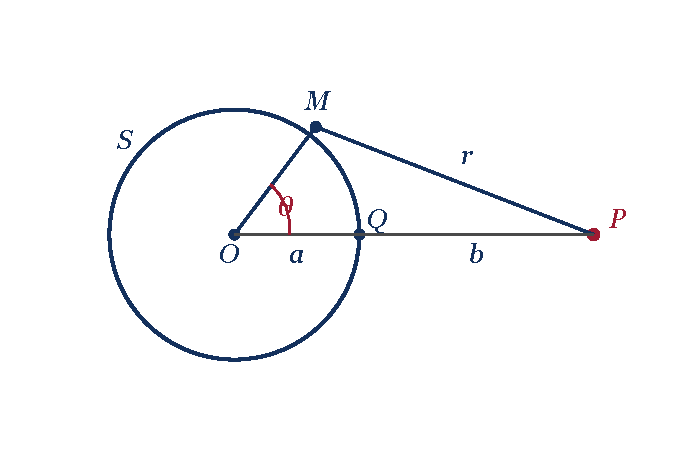
\includegraphics[width=0.7\textwidth]{figuras/pdf/cap04-fig2.pdf}
\caption{Cambio de coordenadas sobre la esfera $S$: el punto $M$, el
centro $O$, el polo $Q$ y el punto iluminado $P$.}
\label{fig:cap4-2}
\end{figure}

Se puede dar a esta expresión otra forma. Designando por $b$ la distancia
$QP$ del punto $P$ a la esfera, tenemos, en el triángulo $MOP$:
\[
r^2=(a+b)^2+a^2-2a(a+b)\cos\theta;
\]
diferenciando, se obtiene
\[
r\,dr = a(a+b)\sin\theta\,d\theta.
\]
Y, si reemplazamos en $d\omega$ el producto $\sin\theta\,d\theta$ por su
valor tomado de esta última expresión, resulta:
\[
d\omega = \frac{a^2r\,dr}{a(a+b)}\,d\varphi = \frac{a}{a+b}\,r\,dr\,d\varphi.
\]
Llevando este valor de $d\omega$ a la expresión (5) de $\xi_0$, obtenemos
\begin{equation}
\xi_0 = \frac{a}{a+b}\iint X\,e^{i\alpha r}\,dr\,d\varphi,
\tag{7}
\end{equation}
tomándose la integración entre $b$ y $2a+b$ para $r$, y entre $0$ y $2\pi$
para $\varphi$.

Sin embargo, no extenderemos la integración más que a la parte de la
esfera $S$ no ocupada por la pantalla; eso no cambiará en nada el
resultado, puesto que sobre la pantalla la función $X$ es nula.
Tendremos así la ventaja de que, en todo el campo de integración, la
función $X$ será continua y sus derivadas serán finitas, lo cual es
necesario para lo que sigue. En estas condiciones, los límites de la
integración respecto de $r$ no serán forzosamente $b$ y $2a+b$. Los
llamaremos $r_1$ y $r_2$.

Integremos primero respecto de $r$. Aplicando la regla de la integración
por partes, y designando por $r_1$ y $r_2$ los límites de la variable,
tendremos
\[
\int X\,e^{i\alpha r}\,dr =
\left[\frac{X\,e^{i\alpha r}}{i\alpha}\right]_{r_1}^{r_2}
-\frac{1}{i\alpha}\int\frac{dX}{dr}\,e^{i\alpha r}\,dr,
\]
y, si integramos por partes la integral del segundo miembro, obtendremos
\[
\int X\,e^{i\alpha r}\,dr =
\left[\frac{X\,e^{i\alpha r}}{i\alpha}\right]_{r_1}^{r_2}
+\frac{1}{\alpha^2}\left[\frac{dX}{dr}\,e^{i\alpha r}\right]_{r_1}^{r_2}
-\frac{1}{\alpha^2}\int\frac{d^2X}{dr^2}\,e^{i\alpha r}\,dr,
\]
siendo $\alpha$ una cantidad infinitamente grande, podemos en general, en
el cálculo aproximado que nos hemos propuesto, despreciar los términos del
segundo miembro que contienen como factor una potencia de $\alpha$
inferior a $-1$. Tenemos entonces
\[
\int X\,e^{i\alpha r}\,dr =
\left[\frac{X\,e^{i\alpha r}}{i\alpha}\right]_{r_1}^{r_2},
\]
y el valor de $\xi_0$ dado por la integral (7) es, aproximadamente,
\begin{equation}
\xi_0 = \frac{a}{a+b}\int_0^{2\pi}
\left[\frac{X\,e^{i\alpha r}}{i\alpha}\right]_{r_1}^{r_2} d\varphi.
\tag{8}
\end{equation}

\noindent\textbf{87.} En la figura~\ref{fig:cap4-2}, el punto $P$ se
encuentra fuera de la esfera $S$; pero es evidente que, si hubiéramos
tomado el punto $P$ dentro de la esfera, habríamos llegado a la misma
expresión de $\xi_0$ considerando, en ese caso, como negativa la distancia
$b$ del punto a la esfera.

Vamos a mostrar, con ayuda de la expresión (8), que el valor de $\xi_0$ es
sensiblemente nulo en un punto interior a la esfera.

Veamos, en efecto, qué representan los límites superior e inferior $r_1$
y $r_2$. Pueden presentarse varios casos; solo consideraremos tres:

1.\textsuperscript{o} No hay pantalla. Se tiene entonces $r_1=b$, $r_2=2a+b$, si el
punto $P$ es exterior a la esfera, y $r_1=b$, $r_2=2a-b$, si el punto $P$
es interior a la esfera.

2.\textsuperscript{o} Hay una pantalla; el punto $Q$, polo del punto $P$, no está en
la pantalla, pero el punto diametralmente opuesto pertenece a ella.

Entonces $r_1=b$; y el límite superior $r_2$, que es en general una
función de $\varphi$, es el valor de $r$ que corresponde al borde de la
pantalla.

3.\textsuperscript{o} Hay una pantalla; el punto $Q$ pertenece a la pantalla, y el
punto diametralmente opuesto no forma parte de ella.

Entonces $r_2=2a\pm b$ y $r_1$ es el valor de $r$ que corresponde al borde
de la pantalla.

Llamemos $J$ a la integral $\displaystyle\int_0^{2\pi}
\dfrac{X\,e^{i\alpha r}}{i\alpha}\,d\varphi$ tomada a lo largo del borde
de la pantalla, y sean $X'$ y $X''$ los valores de
$\dfrac{X\,e^{i\alpha r}}{i\alpha}$ en el punto $Q$ y en el punto
diametralmente opuesto.

Tendremos: en el primer caso,
$\xi_0=\dfrac{a}{a+b}(2\pi X''-2\pi X')$; en el segundo,
$\xi_0=\dfrac{a}{a+b}(J-2\pi X')$; en el tercero,
$\xi_0=\dfrac{a}{a+b}(2\pi X''-J)$.

Veremos más adelante que $J$ es generalmente despreciable.

Nos queda por calcular $X'$ y $X''$. Tenemos
$X=X_2\left(i\alpha+i\alpha\cos\psi-\dfrac{\cos\psi}{r}\right)$. El
último término $\cos\psi/r$ es despreciable frente a $i\alpha$ porque
$\alpha$ es muy grande. Queda, pues,
$X=i\alpha X_2(1+\cos\psi)=-\dfrac{i\alpha\xi_1}{4\pi}(1+\cos\psi)$,
puesto que, fuera de la pantalla, $X_2$ es igual a $-\xi_1/4\pi$.

En el punto $Q$ se tiene: si el punto $P$ es exterior a $S$, $\psi=0$,
$X'=-\dfrac{\xi_1}{2\pi}e^{i\alpha b}$; si el punto $P$ es interior a $S$,
$\psi=\pi$, $X'=0$.

En el punto diametralmente opuesto se tiene, en todos los casos, $\psi=\pi$
y $X''=0$.

Por consiguiente, si el punto $P$ es interior a $S$, la integral (8) será
generalmente despreciable.

\noindent\textbf{88.} Si el punto $P$ es exterior a $S$, se tiene, en los
tres casos considerados más arriba:

En el primer caso, $\xi_0=\xi_1e^{i\alpha b}\dfrac{a}{a+b}$.

En el segundo caso, $\xi_0=\xi_1e^{i\alpha b}\dfrac{a}{a+b}$.

En el tercer caso, $\xi_0=0$.

Luego, si el punto $Q$ no pertenece a la pantalla, es decir, si $P$ no
está en la sombra geométrica, la intensidad es la misma que si no hubiera
pantalla. Si, por el contrario, $P$ está en la sombra geométrica, la
intensidad es nula. En otras palabras, los fenómenos son los mismos que
en la teoría geométrica de las sombras. No habrá, pues, fenómenos de
difracción sino cuando la integral $J$ no sea despreciable.

Nos vemos, pues, llevados a: 1.\textsuperscript{o} demostrar que la integral $J$ es
generalmente despreciable; 2.\textsuperscript{o} buscar cuáles son los casos de
excepción en que deja de serlo.

Tenemos que evaluar la integral
$J=\displaystyle\int \dfrac{X\,e^{i\alpha r}}{i\alpha}\,d\varphi$
extendida a todo el contorno de la pantalla.

Para ello descompondremos ese contorno en cierto número de arcos
parciales, que serán de dos clases:

1.\textsuperscript{o} sobre los arcos de la primera clase, la derivada $d\varphi/dr$
será finita;

2.\textsuperscript{o} sobre los arcos de la segunda clase, esa derivada será lo
bastante grande como para no ser despreciable frente a $\alpha$.

Por lo demás, nada nos impide suponer que la subdivisión del contorno en
arcos parciales se ha hecho de tal modo que, a lo largo de cada uno de
esos arcos, $r$ sea constantemente creciente o constantemente decreciente.

\noindent\textbf{89.} Evaluemos primero la integral tomada a lo largo de
un arco de la primera clase.

Si tomamos como variable de integración $r$, nuestra integral se escribirá:
\[
\int \frac{X\,e^{i\alpha r}}{i\alpha}\,\frac{d\varphi}{dr}\,dr.
\]
Integrando por partes, se tiene
\[
-\frac{X\,e^{i\alpha r}}{\alpha^2}\,\frac{d\varphi}{dr}
+\frac{1}{\alpha^2}\int e^{i\alpha r}\,\frac{d}{dr}
\left(X\,\frac{d\varphi}{dr}\right)dr.
\]
Ahora bien, $X$ es del mismo orden que $\alpha$; si, pues, $d\varphi/dr$
es una cantidad finita, cada uno de los términos de esta última suma es
del orden de $1/\alpha$, es decir, despreciable. Así, la integral tomada a
lo largo de un arco de la primera clase es despreciable.

La integral $\displaystyle\int_{\varphi_0}^{\varphi_1}
\dfrac{X\,e^{i\alpha r}}{i\alpha}\,d\varphi$ tomada a lo largo de un arco
de la segunda clase será también despreciable en general, porque la
diferencia $\varphi_1-\varphi_0$ de los límites de integración será del
mismo orden de magnitud que $1/\alpha$.

Para que la integral $J$ tenga un valor finito, es necesario, pues, que
$\varphi_1-\varphi_0$ sea finito, es decir, que al menos uno de los arcos
de la segunda clase sea visto desde el punto $Q$ bajo un ángulo finito; lo
cual puede ocurrir en dos casos:

1.\textsuperscript{o} si ese arco es en sí mismo finito; se tiene entonces, a lo largo
de todo ese arco, $d\varphi/dr=\infty$, $dr/d\varphi=0$, $r=\text{const.}$;
es decir, que el arco en cuestión debe diferir muy poco de un arco de
círculo con polo en $Q$.

2.\textsuperscript{o} si ese arco pasa muy cerca del punto $Q$, es decir, si ese punto
está muy próximo al borde de la pantalla.

Cada vez que no sea así, la integral $J$ será despreciable y no tendremos
otros fenómenos que los previstos por la teoría geométrica de las
sombras.

\noindent\textbf{90.} Busquemos, pues, en qué casos $d\varphi/dr$ es
infinito. Hallamos en el §86 $r\,dr=a(a+b)\sin\theta\,d\theta$; de donde
deducimos\footnote{En el original no hay ninguna ecuación numerada (9)
en esta serie: la numeración pasa directamente de la (8) del §86 a la
(10). Conservamos la numeración de Poincaré.~(N.~del T.)}
\begin{equation}
\frac{d\varphi}{dr} = \frac{1}{a(a+b)}\,\frac{r}{\sin\theta}\,
\frac{d\varphi}{d\theta}.
\tag{10}
\end{equation}
Esta igualdad nos muestra que $d\varphi/dr$ podrá volverse infinita en dos
casos: 1.\textsuperscript{o} si $\sin\theta$ es muy pequeño; 2.\textsuperscript{o} si
$d\varphi/d\theta$ es infinito.

Consideremos el primer caso. Siendo muy pequeño el ángulo $\theta$, un
arco del contorno de la pantalla está muy próximo al punto $Q$, y se puede
confundir la porción de la esfera que contiene ese arco con un plano que
pase por $Q$. Además, siendo infinitamente pequeño ese arco, se le puede
considerar como un elemento de una recta $AB$ (figura~\ref{fig:cap4-3}).
La distancia del punto $Q$ al elemento de arco $M$ es $a\theta$, siendo
$a$ el radio de la esfera sobre la que se encuentra la porción
considerada del contorno de la pantalla. Llamando $a\delta$ a la distancia
más corta $QC$ del punto $Q$ a la recta $AB$, y $\varphi$ al ángulo de
$QM$ y $QC$, tenemos
\[
a\theta\cos\varphi = a\delta \qquad\text{o bien}\qquad \theta\cos\varphi=\delta.
\]

\begin{figure}[htbp]
\centering
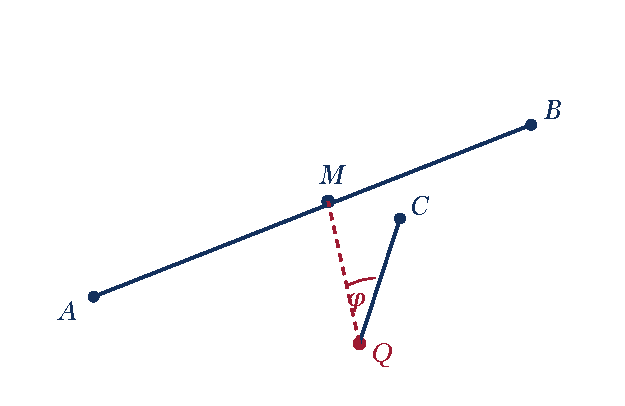
\includegraphics[width=0.6\textwidth]{figuras/pdf/cap04-fig3.pdf}
\caption{El arco del borde de la pantalla, confundido con la recta $AB$
cerca del polo $Q$; distancia $QC=a\delta$ y ángulo $\varphi$.}
\label{fig:cap4-3}
\end{figure}

El ángulo $\varphi$ que consideramos aquí no difiere, por lo demás, más
que en una constante del ángulo designado antes con la misma letra; sus
diferenciales tendrán, pues, el mismo valor. Diferenciando los dos
miembros de la igualdad anterior, hallamos
\[
\frac{d\theta}{d\varphi}\cos\varphi - \theta\sin\varphi = 0,
\]
nueva igualdad que nos muestra que $d\theta/d\varphi$ es del mismo orden
que $\theta$, y por tanto que $\delta$. Por consiguiente, $d\varphi/d\theta$
es del orden de $1/\delta$, y $d\varphi/dr$, dado por la relación (10), es
del orden de $r/\delta^2$.

Si el punto $P$ está a una distancia finita $r$ de la esfera, $d\varphi/dr$
es del orden de $1/\delta^2$, y, si se quiere que esta derivada sea del
mismo orden que $1/\lambda$, es necesario que $\delta$ sea del orden de
$\sqrt{\lambda}$. Si, por el contrario, el punto $P$ está a una distancia
de la esfera del orden de $\lambda$, será necesario que $\delta$ sea del
mismo orden que $\lambda$ para que $d\varphi/dr$ sea un infinito del orden
de $1/\lambda$.

La recta que une el punto $P$ con la fuente luminosa deberá, pues,
encontrar la esfera a una distancia del contorno de la pantalla del orden
de $\lambda$ para que haya en $P$ una iluminación anómala; la región en
que debe hallarse el punto $P$ es entonces demasiado pequeña para ser
observable. No se podrán observar anomalías en la iluminación de $P$ sino
cuando este se halle a una distancia finita de la esfera.

Así, sobre una esfera concéntrica a $S$, de radio $a+b$, siendo $b$
finito, la región ocupada por las franjas de difracción es del mismo
orden de magnitud que $\sqrt{\lambda}$. Sobre la esfera $S$ misma, esa
región es del mismo orden de magnitud que $\lambda$.

\noindent\textbf{91.} Examinemos el segundo caso, en el cual $d\varphi/dr$
es una cantidad infinitamente grande; siendo infinito $d\theta/d\varphi$,
$d\varphi/d\theta$ debe ser infinitamente pequeño. Si, pues, $r/\sin\theta$
es una cantidad finita, será necesario, para que $d\varphi/dr$ sea del
orden de $1/\lambda$, que $d\theta/d\varphi$ sea del orden de $\lambda$.

Es necesario, en otros términos, que $\theta$ sea constante salvo
cantidades del orden de $\lambda$, es decir que, despreciando las
cantidades de ese orden, un arco finito del contorno de la pantalla pueda
considerarse como un arco de círculo con centro en $Q$; la distancia del
punto $Q$ al centro de curvatura medio de ese arco debe ser, pues, del
orden de $\lambda$; de ahí resulta que los puntos iluminados de manera
anómala están todos contenidos dentro de un círculo cuyo radio es del
orden de $\lambda$, y que los fenómenos son inobservables.

Es necesario, pues, para que la observación sea posible, que $\sin\theta$,
y por consiguiente el radio de ese arco de círculo, sean muy pequeños.

Si $\sin\theta/r$ es una cantidad del orden de $\sqrt{\lambda}$, bastará
que $d\theta/d\varphi$ sea del orden de $\lambda$, y, por tanto, que la
distancia del punto $Q$ al centro del arco de círculo sea también del
mismo orden.

La región del espacio en la que debe situarse el punto $P$ para presentar
fenómenos anómalos es entonces lo bastante grande como para poder
observar esos fenómenos.

Observemos que, si el punto $P$ está situado sobre la esfera, su
iluminación quedará determinada por la teoría geométrica de las sombras,
o al menos la observación será incapaz de detectar una diferencia entre
la iluminación así determinada y la iluminación real.

Se tendrá, en efecto, cuando el punto $P$ tiende al punto $Q$,
$\sin\theta/r=1/a$, pues, en el triángulo $MOP$, se tiene
$\sin\theta/r=\sin OMP/a$, y en el límite el ángulo $OMP$ es recto. Siendo
finito $\sin\theta/r$, resultará aún, según lo que acabamos de ver, que
los fenómenos no serán observables.

\noindent\textbf{92.} Vamos a mostrar ahora que la condición de
transversalidad $\Theta_0=\xi_0'+\eta_0'+\zeta_0'=0$ se cumple para los
puntos $P$ situados fuera de la esfera $S$, o sobre esa misma esfera.

En efecto, $\Theta_0$ satisface la ecuación $\Delta\Theta_0+\alpha^2\Theta_0=0$.

Tenemos, pues, fuera de la esfera $S$, según el §81,
\[
\Theta_0 = -\int \frac{\Theta_0}{4\pi}\,\frac{e^{i\alpha r}}{r}
\left(i\alpha-\frac1r\right)\cos\psi\,d\omega +
\int \frac{1}{4\pi}\,\frac{d\Theta_0}{dn}\,\frac{e^{i\alpha r}}{r}\,d\omega,
\]
extendiéndose las integrales del segundo miembro a todos los elementos
$d\omega$ de la esfera $S$.

Ahora bien, vimos que, dejando de lado la región en que hay franjas de
difracción, los fenómenos son los mismos que en la teoría geométrica de
las sombras; en otras palabras, la iluminación es nula en ciertos puntos
y en otros es la misma que si no hubiera pantalla. En ambos casos,
$\Theta_0$ y $d\Theta_0/dn$ son nulos.

Bastará, pues, con el grado de aproximación adoptado, extender las
integrales del segundo miembro a la región de la esfera $S$ ocupada por
las franjas; ahora bien, vimos que esa región es del orden de $\lambda$.
Las integrales del segundo miembro son, pues, despreciables, y, por
consiguiente, lo mismo ocurre con $\Theta_0$.

En resumen, las integrales (4) satisfacen bien las condiciones A, B, C, D,
y no puede haber iluminación anómala sino cuando el punto $P$ está muy
próximo al borde de la sombra geométrica.

\noindent\textbf{93. Simplificación de las expresiones $\xi_0,\eta_0,\zeta_0$.}
— Vimos que, si el punto $Q$ está a una distancia finita de los bordes de
una pantalla, la iluminación del punto $P$ es la misma que en la teoría de
las sombras, y, en segundo lugar, que la iluminación se modifica si el
punto $Q$ está a una distancia de la pantalla del orden de $\sqrt{\lambda}$.
La iluminación de un punto no depende, pues, apenas más que de las
porciones de la esfera vecinas al punto $Q$. Este punto se llama el
\emph{polo} del punto $P$. Vamos a aprovechar esta observación para
simplificar los valores de $\xi_0,\eta_0,\zeta_0$ dados por las
integrales (4).

Tomemos la primera de esas integrales,
\[
\xi_0 = \int X_2\,d\omega\,\frac{e^{i\alpha r}}{r}
\left(i\alpha+i\alpha\cos\psi-\frac{\cos\psi}{r}\right).
\]
Puesto que las partes de esta integral que no son despreciables son las
que corresponden a los puntos muy próximos al polo $Q$ del punto iluminado
$P$, no extenderemos la integral sino a esos puntos, y podremos considerar
$X_2$ y $\psi$ como constantes. Como, además, $\alpha$ es una cantidad muy
grande y $r$ debe ser finito para que los fenómenos de difracción sean
observables, podemos, en la cantidad colocada bajo el signo de
integración, despreciar el término $\cos\psi/r$ frente a los otros dos
términos $i\alpha$ y $i\alpha\cos\psi$. Haciendo esta simplificación, y
sacando fuera de la integral los términos considerados como constantes,
tenemos
\[
\xi_0 = X_2\,i\alpha(1+\cos\psi)\int \frac{e^{i\alpha r}}{r}\,d\omega.
\]
Se sabe, por lo demás (§84), que $X_2=-\xi_1/4\pi$; por consiguiente,
reemplazando, en la expresión de $\xi_0$, $X_2$ y $\cos\psi$ por los
valores de esas cantidades en el polo $Q$, tendremos
\[
\xi_0 = -\frac{i\alpha}{2\pi}\,\xi_1 \int \frac{e^{i\alpha r}}{r}\,d\omega.
\]
La distancia $r$ del punto $P$ a los puntos de la esfera que están
próximos al polo $Q$ difiere muy poco de la distancia $PQ=b$, y, por
tanto, puede sacarse fuera de la integral, puesto que esta no se extiende
más que a los puntos vecinos de $Q$. El valor de $\xi_0$ se convertirá en
\[
\xi_0 = -\frac{i\alpha}{2\pi}\,\frac{\xi_1}{b}\int e^{i\alpha r}\,d\omega,
\]
y por último, mediante una última transformación,
\[
\xi_0 = -\frac{i\alpha\xi_1e^{i\alpha b}}{2\pi b}
\int e^{i\alpha(r-b)}\,d\omega.
\]

\noindent\textbf{94.} Busquemos el valor de esta última integral. Tenemos,
en el triángulo $MOP$ (figura~\ref{fig:cap4-2}),
$r^2=(a+b)^2+a^2-2a(a+b)\cos\theta$; y, como solo tenemos que considerar
puntos vecinos del polo $Q$, para los cuales $\theta$ es muy pequeño,
podemos reemplazar $\cos\theta$ por los dos primeros términos
$1-\theta^2/2$ de su desarrollo; tendremos
$r^2=(a+b)^2+a^2-2a(a+b)(1-\theta^2/2)$, o bien
$r^2=(a+b-a)^2+a(a+b)\theta^2=b^2+a(a+b)\theta^2$.

Designando por $s$ el arco de círculo máximo $QM$ comprendido entre un
punto $M$ de la esfera y el polo $Q$, tendremos $\theta\approx s/a$; y,
llevando este valor de $\theta$ a la expresión de $r^2$, resultará
$r^2=b^2+\dfrac{a+b}{a}s^2$. De ahí se obtiene,
$r-b=\dfrac{a+b}{a(r+b)}s^2$.

Pero, difiriendo $r$ muy poco de $b$, se puede reemplazar $r+b$ por $2b$,
de modo que se tiene $r-b=\dfrac{a+b}{2ab}s^2$.

Este valor de $r-b$, llevado a la expresión de $\xi_0$, da
\[
\xi_0 = -\frac{i\alpha\xi_1e^{i\alpha b}}{2\pi b}
\int e^{i\alpha\frac{a+b}{2ab}s^2}\,d\omega.
\]
No debiendo extenderse la integral más que a las porciones de la esfera
que rodean al punto $Q$, se pueden considerar esas porciones situadas en
el plano tangente a la esfera en $Q$. Tomemos, en ese plano, dos ejes de
coordenadas rectangulares que se cortan en $Q$. En este sistema, las
coordenadas del punto $M$ serán las distancias $l$ y $l'$ de ese punto a
los ejes. Para simplificar la expresión de $\xi_0$, definiremos la
posición del punto $M$ mediante dos parámetros $u$ y $v$ tales que
\[
l=u\sqrt{\frac{ab\lambda}{2(a+b)}},\qquad
l'=v\sqrt{\frac{ab\lambda}{2(a+b)}}.
\]
Se tiene entonces $s^2=l^2+l'^2=(u^2+v^2)\dfrac{ab\lambda}{2(a+b)}$, y
$d\omega=dl\,dl'=du\,dv\,\dfrac{ab\lambda}{2(a+b)}$.

Llevando estos valores de $s^2$ y de $d\omega$ a la expresión de $\xi_0$,
tendremos, tras las simplificaciones,
\[
\xi_0 = -\frac{i\alpha\xi_1a\lambda e^{i\alpha b}}{4\pi(a+b)}
\int e^{\frac14 i\alpha\lambda(u^2+v^2)}\,du\,dv,
\]
y, como habíamos puesto $\alpha=2\pi/\lambda$, obtenemos, reemplazando
$\alpha$ por ese valor,
\begin{equation}
\xi_0 = -\frac{ia\xi_1e^{i\alpha b}}{2(a+b)}
\int e^{\frac{i\pi}{2}(u^2+v^2)}\,du\,dv.
\tag{11}
\end{equation}

\section{Intensidad luminosa en un punto}

\noindent\textbf{95. Intensidad luminosa en un punto.} — Según lo dicho en
el §76, la componente según el eje $x$ del desplazamiento de un punto $P$
situado fuera de la esfera $S$ es $\xi=$ parte real de $\xi_0e^{-i\alpha Vt}$,
donde $\xi_0$ se reemplaza por la expresión (11) que acabamos de hallar.
Tendríamos para las otras dos componentes las cantidades
$\eta=$ parte real de $\eta_0e^{-i\alpha Vt}$,
$\zeta=$ parte real de $\zeta_0e^{-i\alpha Vt}$, deduciéndose $\eta_0$ y
$\zeta_0$ de $\xi_0$ al reemplazar, en la expresión (11), $\xi_1$ por
$\eta_1$ o $\zeta_1$. La intensidad luminosa en el punto $P$ será, pues,
proporcional a
$\rho\!\left[\!\left(\dfrac{d\xi}{dt}\right)^2+\!
\left(\dfrac{d\eta}{dt}\right)^2+\!\left(\dfrac{d\zeta}{dt}\right)^2\right]$;
ahora bien, se tiene
\[
\frac{d\xi}{dt} = \text{parte real de }
\left(-i\alpha V\xi_0e^{-i\alpha Vt}+e^{-i\alpha Vt}\frac{d\xi_0}{dt}\right)
\]
y dos expresiones análogas para $d\eta/dt$ y $d\zeta/dt$. Por
consiguiente, la intensidad es proporcional a la suma de los cuadrados de
los módulos de las tres cantidades análogas a
$\left(-i\alpha V\xi_0+\dfrac{d\xi_0}{dt}\right)$.

Pero, en el valor (11) de $\xi_0$, la única cantidad que depende del
tiempo es $\xi_1$, de modo que la intensidad es igual a la suma de los
cuadrados de los módulos de tres cantidades, de las cuales la
primera es\footnote{El original inicia aquí la tercera serie de numeración
de ecuaciones del capítulo; las (1) a (7) de los §§95-99 no
deben confundirse con las de los §§76-82 ni con las de los §§83-94.
Conservamos la numeración de Poincaré.~(N.~del T.)}
\begin{equation}
\left(-i\alpha V\xi_1+\frac{d\xi_1}{dt}\right)
\frac{ia\,e^{i\alpha b}}{2(a+b)}
\int e^{\frac{i\pi}{2}(u^2+v^2)}\,du\,dv,
\tag{1}
\end{equation}
y de las cuales las otras dos se deducen de esta reemplazando $\xi_1$ por
$\eta_1$ y $\zeta_1$.

Observándose los fenómenos de difracción en un plano, tenemos que
considerar la intensidad relativa de los puntos situados en un mismo
plano. Estando esos puntos siempre vecinos entre sí y a cierta distancia
de la pantalla, podemos admitir que las distancias $b$ de cada uno de
ellos a la esfera que contiene la pantalla son las mismas. De ello
resulta que, en cada uno de los términos (1), cuya suma de cuadrados es
proporcional a la intensidad, el factor $\dfrac{ia\,e^{i\alpha b}}{2(a+b)}$
es el mismo para esos puntos, si solo se considera luz homogénea. Además,
como esos puntos se observan en el mismo instante y los valores de
$\xi_1,\eta_1,\zeta_1$ varían poco al pasar de un punto de la esfera $S$ a
un punto vecino, el factor $\left(-i\alpha V\xi_1+\dfrac{d\xi_1}{dt}\right)$
tendrá sensiblemente el mismo valor. La intensidad relativa de la luz en
los distintos puntos observados será, pues, proporcional, en el mismo
instante, al cuadrado del módulo de la integral,
\begin{equation}
\int e^{\frac{i\pi}{2}(u^2+v^2)}\,du\,dv,
\tag{2}
\end{equation}
que aparece como factor en el término (1) y en los dos que de él se
deducen. Nos bastará, pues, para hallar la intensidad luminosa en los
diversos puntos del plano donde se hacen las observaciones, estudiar las
variaciones del módulo de esta integral.

\section{Expresión de la integral en el caso de una rendija de bordes
paralelos}

\noindent\textbf{96. Expresión de la integral (2) en el caso de una
rendija de bordes paralelos.} — Supondremos que uno de los ejes a los que
corresponden los parámetros $u$ y $v$ sea paralelo a los bordes de la
rendija; sea ese el eje de las $u$, por ejemplo. Si nos remitimos a la
relación $\delta=u\sqrt{\dfrac{ab\lambda}{2(a+b)}}$, que liga el parámetro
$u$ con la distancia $\delta$ de un punto del plano $uv$ al eje de las
$v$, se ve que $u$ es del orden de $\delta/\sqrt{\lambda}$. Teniendo la
rendija una longitud, si no ilimitada, al menos muy grande respecto de las
cantidades del orden de $\sqrt{\lambda}$, los valores de $u$ serán siempre
muy grandes para los puntos que se observan. Por consiguiente, se pueden,
en la integral (2), considerar como infinitos los límites de $u$.
Designaremos por $v_1$ y $v_2$ los límites de $v$, que tienen en general
valores finitos, siendo pequeña la anchura de la rendija. Podemos poner
esta integral, cuyos límites son constantes, bajo la forma
\[
\int_{-\infty}^{+\infty} e^{\frac{i\pi}{2}u^2}\,du
\int_{v_1}^{v_2} e^{\frac{i\pi}{2}v^2}\,dv.
\]
La primera de estas integrales tiene por valor $1+i$, cuyo módulo es
$\sqrt2$;\footnote{El original dice «dont le module est 2»; es una errata
evidente, pues el módulo de $1+i$ es $\sqrt2$: es su cuadrado, que es lo
que interviene en la intensidad, el que vale $2$.~(N.~del T.)}
de modo que solo tenemos que ocuparnos de la segunda, que se convierte,
cuando se reemplaza en ella la exponencial por las funciones
trigonométricas, en
\begin{equation}
\int_{v_1}^{v_2} e^{\frac{i\pi}{2}v^2}\,dv =
\int_{v_1}^{v_2}\cos\frac{\pi v^2}{2}\,dv +
i\int_{v_1}^{v_2}\sin\frac{\pi v^2}{2}\,dv.
\tag{3}
\end{equation}

\section{Representación gráfica de la integral de Fresnel}

\noindent\textbf{97. Representación gráfica de la integral (3).} — Las
dos integrales del segundo miembro son conocidas con el nombre de
\emph{integrales de Fresnel}; vamos a estudiarlas. Para simplificar los
cálculos, supondremos nulo el límite inferior de estas integrales; será
fácil después pasar al caso general, en que los límites son cualesquiera,
tomando la suma algebraica de dos integrales de las cuales uno de los
límites es $0$.

Pongamos, pues,
\[
x=\int_0^v \cos\frac{\pi v^2}{2}\,dv,\qquad
y=\int_0^v \sin\frac{\pi v^2}{2}\,dv,
\]
y construyamos la curva lugar geométrico de los puntos de coordenadas $x$
e $y$. Pasa por el origen de coordenadas, pues se tiene $x=y=0$ para
$v=0$. Si se cambia $v$ por $-v$, el elemento de las integrales no
cambia, pero el límite superior cambia de signo, y $x$ e $y$ cambian a la
vez de signo; el origen es, pues, un centro de simetría de la curva.

Tomemos las diferenciales de $x$ y de $y$: tenemos
$dx=\cos\dfrac{\pi v^2}{2}\,dv$, $dy=\sin\dfrac{\pi v^2}{2}\,dv$. Elevando
al cuadrado y sumando, obtenemos $dx^2+dy^2=ds^2=dv^2$; luego $ds=dv$,
siendo $ds$ un elemento de arco de la curva. Integrando los dos miembros
de esta igualdad y tomando $0$ como constante de integración, lo cual
equivale a contar los arcos a partir del origen, puesto que $x=y=0$ para
$v=0$, se tiene $s=v$.

El cociente $dy/dx$ da la tangente del ángulo formado por el eje de las
$x$ y la tangente a la curva en el punto $x,y$; designando por $\omega$
ese ángulo,\footnote{Poincaré designa este ángulo por $\alpha$; lo
llamamos $\omega$ para no confundirlo con $\alpha=2\pi/\lambda$.~(N.~del T.)} tenemos
\begin{equation}
\omega = \frac{\pi}{2}v^2.
\tag{4}
\end{equation}
El radio de curvatura en un punto viene dado por
$\dfrac{ds}{d\omega}=\dfrac{dv}{\pi v\,dv}=\dfrac{1}{\pi v}$; en el
origen, es decir, para $v=0$, el radio de curvatura es infinito, y, como
$\omega$ es nulo a la vez que $v$, el eje de las $x$ es una tangente de
inflexión en el punto $O$ (figura~\ref{fig:cap4-4}).

\begin{figure}[htbp]
\centering
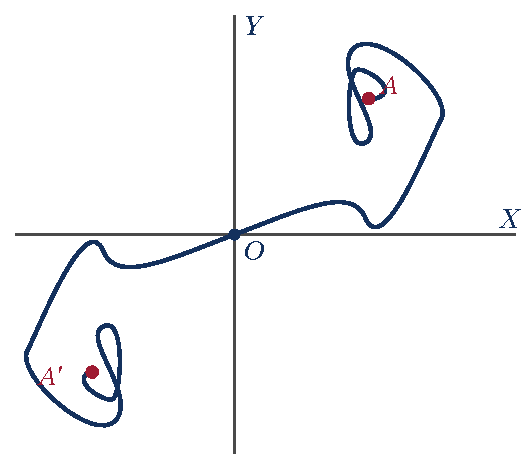
\includegraphics[width=0.7\textwidth]{figuras/pdf/cap04-fig4.pdf}
\caption[La espiral de Fresnel y sus dos puntos asintóticos $A$ y
$A'$.]{La espiral de Fresnel: la curva de coordenadas $x=\int_0^v
\cos(\pi v^2/2)\,dv$, $y=\int_0^v\sin(\pi v^2/2)\,dv$, con sus dos puntos
asintóticos $A$ y $A'$.}
\label{fig:cap4-4}
\end{figure}

Para construir la curva, haremos variar $v$ de $0$ a infinito; el ángulo
$\omega$ de la tangente a la curva con el eje $ox$ aumentará más allá de
todo límite; el radio de curvatura tenderá a $0$. Tendremos, pues, una
curva en forma de caracol, con un punto asintótico. Busquemos las
coordenadas de ese punto $A$. Para ello, busquemos el valor de la
integral $\displaystyle\int_0^\infty e^{\frac{i\pi}{2}v^2}\,dv$.

Se sabe que se tiene $\displaystyle\int_0^\infty e^{-z^2}\,dz=\frac12\sqrt\pi$.

Si ponemos $z^2=-\dfrac{i\pi}{2}v^2$, tenemos $z=v\sqrt{-i\pi/2}$,
$dz=dv\sqrt{-i\pi/2}$.

Por consiguiente, tendremos, para la integral buscada,
\[
\int_0^\infty e^{\frac{i\pi}{2}v^2}\,dv =
\frac12\sqrt\pi\,\sqrt{-\frac{2}{i\pi}} = \frac12\sqrt{2i} = \frac{1+i}{2};
\]
ahora bien, $\displaystyle\int_0^v e^{\frac{i\pi}{2}v^2}\,dv=x+iy$, luego,
para $v=\infty$, tenemos $x=\dfrac12$, $y=\dfrac12$.

Tales son las coordenadas del punto asintótico $A$. Se obtendrá la parte
de la curva correspondiente a valores negativos de $v$ por simetría.

\noindent\textbf{98.} Para definir mejor la curva, podemos buscar cómo
varía la distancia $AM$ del punto asintótico $A$ a un punto cualquiera $M$
de la parte de la curva correspondiente a los valores positivos de $v$.

Sea $v$ el valor del parámetro correspondiente a ese punto; sus
coordenadas serán $x=\int_0^v\cos(\pi v^2/2)\,dv$,
$y=\int_0^v\sin(\pi v^2/2)\,dv$.

Traslademos el origen de los ejes de coordenadas al punto $M$; la
abscisa del punto asintótico $A$ respecto de estos nuevos ejes será igual
a su abscisa respecto de los antiguos ejes, disminuida en la abscisa del
punto $M$, es decir,
\[
\int_0^\infty\cos\frac{\pi v^2}{2}\,dv - \int_0^v\cos\frac{\pi v^2}{2}\,dv
= \int_v^\infty \cos\frac{\pi v^2}{2}\,dv.
\]
La ordenada del punto $A$ respecto de los nuevos ejes se obtendrá del
mismo modo, y tendremos $\displaystyle\int_v^\infty\sin\frac{\pi v^2}{2}\,dv$.

Las coordenadas del punto asintótico respecto de los ejes trazados por
$M$ estarán, pues, dadas por la parte real y la parte imaginaria de la
integral
\begin{equation}
J = \int_v^\infty e^{\frac{i\pi}{2}v^2}\,dv.
\tag{5}
\end{equation}
Vamos a buscar otra expresión de $J$. Para ello nos serviremos de nuevo
de la integral $\displaystyle\int_0^\infty e^{-z^2}\,dz=\frac12\sqrt\pi$.
Si ponemos $z=vw$, donde $v$ se supone positivo, tendremos,
$\displaystyle\int_0^\infty e^{-v^2w^2}\,v\,dw=\frac12\sqrt\pi$.

El producto de esta integral por la integral (5) dará
\[
\int_v^\infty\!\int_0^\infty e^{v^2\left(\frac{i\pi}{2}-w^2\right)}
v\,dv\,dw = \frac{J}{2}\sqrt\pi.
\]
Integremos la integral doble del primer miembro respecto de $v$;
tendremos
\[
\int_v^\infty e^{v^2\left(\frac{i\pi}{2}-w^2\right)} v\,dv =
\frac{1}{i\pi-2w^2}\int_v^\infty
d\!\left(e^{v^2\left(\frac{i\pi}{2}-w^2\right)}\right),
\]
o bien
\[
\int_v^\infty e^{v^2\left(\frac{i\pi}{2}-w^2\right)} v\,dv =
-\frac{1}{i\pi-2w^2}\,e^{v^2\left(\frac{i\pi}{2}-w^2\right)}.
\]
La integral doble se convierte, pues, en
\[
\int_0^\infty \frac{e^{v^2\left(\frac{i\pi}{2}-w^2\right)}}{2w^2-i\pi}\,dw
= e^{\frac{i\pi}{2}v^2}\int_0^\infty \frac{e^{-v^2w^2}}{2w^2-i\pi}\,dw
= \frac{J}{2}\sqrt\pi.
\]
Deducimos de ello una nueva expresión de $J$, que nos muestra que las
coordenadas del punto $A$ respecto de los ejes trazados por $M$
paralelamente a los ejes $ox$ y $oy$ son las partes real e imaginaria de
\begin{equation}
J = \frac{e^{\frac{i\pi}{2}v^2}}{\sqrt\pi}
\int_0^\infty \frac{2e^{-v^2w^2}}{2w^2-i\pi}\,dw.
\tag{6}
\end{equation}

\noindent\textbf{99.} Si ahora hacemos girar los ejes alrededor del
punto $M$ en un ángulo igual a $\dfrac{\pi}{2}v^2$, es decir, según la
relación (4), en un ángulo igual al que forma la tangente a la curva en
$M$ con el eje $ox$, tendremos un nuevo sistema de ejes formado por la
tangente y la normal a la curva en el punto $M$. Designemos por $x'$ e
$y'$ las coordenadas de un punto en este nuevo sistema, y por $x_1$ e
$y_1$ las coordenadas del mismo punto en el sistema de ejes paralelos a
$ox$ y $oy$ y que pasan por $M$. Tendremos las fórmulas de transformación
\[
x' = x_1\cos\frac{\pi v^2}{2} + y_1\sin\frac{\pi v^2}{2},\qquad
y' = y_1\cos\frac{\pi v^2}{2} - x_1\sin\frac{\pi v^2}{2}.
\]
Multiplicando la segunda por $i$ y sumando el resultado con la primera,
obtenemos
\[
x'+iy' = (x_1+iy_1)\cos\frac{\pi v^2}{2} - (ix_1-y_1)\sin\frac{\pi v^2}{2}
\]
o bien
\[
x'+iy' = (x_1+iy_1)\left(\cos\frac{\pi v^2}{2}-i\sin\frac{\pi v^2}{2}\right)
\]
o, por último,
\[
x'+iy' = (x_1+iy_1)\,e^{-\frac{i\pi v^2}{2}}.
\]
Esta última relación nos muestra que el imaginario $x'+iy'$ en el nuevo
sistema de ejes es igual a su valor $x_1+iy_1$ en el antiguo, multiplicado
por el factor $e^{-\frac{i\pi v^2}{2}}$. Ahora bien, para el punto
asintótico $A$ se tiene $x_1+iy_1=J$; por consiguiente, tendremos
$x'+iy'=Je^{-\frac{i\pi v^2}{2}}$, y la igualdad (6) nos muestra que
\begin{equation}
x'+iy' = \int_0^\infty \frac{2e^{-v^2w^2}}{\sqrt\pi\left(2w^2-i\pi\right)}\,dw.
\tag{7}
\end{equation}
Multiplicando los dos términos de la fracción colocada bajo el signo de
integración por la cantidad imaginaria conjugada del denominador,
obtenemos
\[
\int_0^\infty \frac{2(2w^2+i\pi)\,e^{-v^2w^2}}{\sqrt\pi(4w^4+\pi^2)}\,dw.
\]
La distancia del punto $A$ a la normal en $M$, que es la parte real de
esta integral, tendrá por expresión
\[
\int_0^\infty \frac{4w^2e^{-v^2w^2}}{\sqrt\pi(4w^4+\pi^2)}\,dw;
\]
y la distancia a la tangente, que es su parte imaginaria, será
\[
\int_0^\infty \frac{2\pi\,e^{-v^2w^2}}{\sqrt\pi(4w^4+\pi^2)}\,dw.
\]
Los elementos de cada una de estas dos últimas integrales son positivos y
decrecen cuando $v$ varía de $0$ a $\infty$. Por consiguiente, las
distancias del punto $A$ a la normal y a la tangente en $M$ son siempre
positivas y decrecientes. Resulta de ello que la distancia $AM$ va
siempre decreciendo. En efecto, si no fuera así, esa distancia
presentaría un máximo o un mínimo. En el punto correspondiente a ese
máximo o a ese mínimo, $AM$ sería normal a la curva, y la distancia del
punto $A$ a la normal sería nula, lo cual no puede ser según lo anterior.

Se puede ver que, para los puntos de la curva vecinos del punto $A$, la
recta $AM$ es sensiblemente normal a la curva. Para esos puntos, $v$ es
muy grande, y la exponencial $e^{-v^2w^2}$ es muy pequeña, a menos que
$w$ no sea pequeño; se podrá, pues, en la integral (7), despreciar los
elementos que no corresponden a un valor pequeño de $w$. Pero, si $w$ es
pequeño, el denominador $2w^2-i\pi$ se reduce sensiblemente a $-i\pi$, de
modo que el valor de $x'+iy'$ es aproximadamente
\[
\frac{2i}{\pi\sqrt\pi}\int_0^\infty e^{-v^2w^2}\,dw =
\frac{2i}{\pi\sqrt\pi}\,\frac12\,\frac{\sqrt\pi}{v} = \frac{i}{\pi v}.
\]
Siendo nula la parte real, la distancia del punto $A$ a la normal es
nula, es decir, que $AM$ es sensiblemente normal. El valor de $AM$ es
aproximadamente $\dfrac{1}{\pi v}$.

La forma de la curva queda entonces suficientemente bien determinada.

\section{Difracción producida por una rendija estrecha}

\noindent\textbf{100. Difracción producida por una rendija estrecha.} —
Hemos visto en el §96 que la intensidad luminosa en un punto exterior es
proporcional al cuadrado del módulo de la integral
\[
\int_{v_1}^{v_2} e^{\frac{i\pi}{2}v^2}\,dv.
\]
El módulo de esta integral es igual a la diferencia geométrica de los
módulos de las integrales
\[
\int_0^{v_2} e^{\frac{i\pi}{2}v^2}\,dv,\qquad
\int_0^{v_1} e^{\frac{i\pi}{2}v^2}\,dv.
\]
Si $M_1$ (figura~\ref{fig:cap4-5}) es el punto de la curva representativa
que corresponde a $v_1$, $M_2$ el que corresponde a $v_2$, los módulos de
estas integrales serán $OM_1$ y $OM_2$; su diferencia geométrica es
$M_1M_2$.

Si se considera un punto $P$ iluminado por una rendija, las cantidades
$v_1$ y $v_2$ son proporcionales a las distancias que separan su polo $Q$
de los bordes de la rendija; como el ancho de la rendija es constante, la
diferencia $v_1-v_2$ tiene siempre el mismo valor cualquiera que sea el
punto $P$ considerado en el plano de observación. Ahora bien, hemos visto
que $v_1$ y $v_2$ son iguales a las longitudes de los arcos de curva
$OM_1$ y $OM_2$; por consiguiente, el arco $M_1M_2$ tiene siempre la misma
longitud. Deberemos, pues, para obtener las variaciones de la intensidad
luminosa en los distintos puntos del plano de observación, buscar las
variaciones de la longitud de una cuerda $M_1M_2$ que subtiende arcos
iguales.

\begin{figure}[ht]
\centering
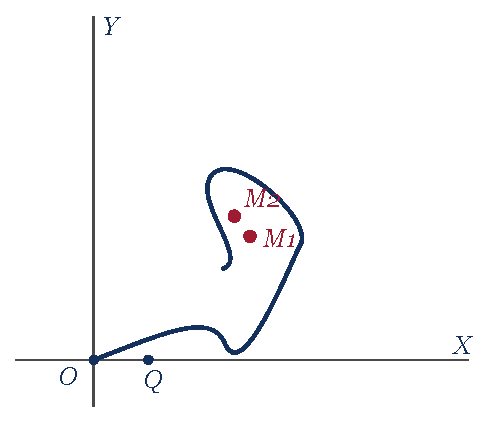
\includegraphics[width=0.55\textwidth]{figuras/pdf/cap04-fig5.pdf}
\caption{Puntos $M_1$, $M_2$ sobre la espiral, correspondientes a los
límites $v_1$, $v_2$ de la integral de Fresnel.}
\label{fig:cap4-5}
\end{figure}

Para que haya máximo o mínimo, es necesario que el triángulo formado por
la cuerda y las tangentes $M_1T$ y $M_2T$ (figura~\ref{fig:cap4-6}) sea
isósceles, o bien que las tangentes en los extremos sean paralelas y del
mismo sentido (figura~\ref{fig:cap4-7}). Tendremos así dos categorías de
máximos y de mínimos.

\begin{figure}[ht]
\centering
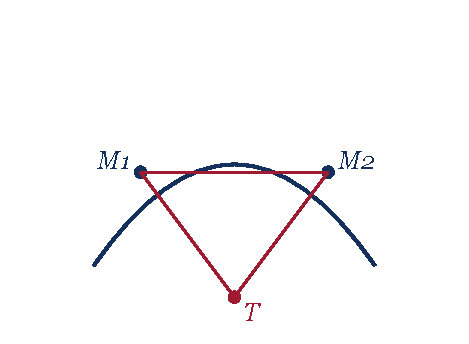
\includegraphics[width=0.55\textwidth]{figuras/pdf/cap04-fig6.pdf}
\caption{Triángulo isósceles formado por la cuerda $M_1M_2$ y las
tangentes que se cortan en $T$: primera categoría de extremos.}
\label{fig:cap4-6}
\end{figure}

\begin{figure}[ht]
\centering
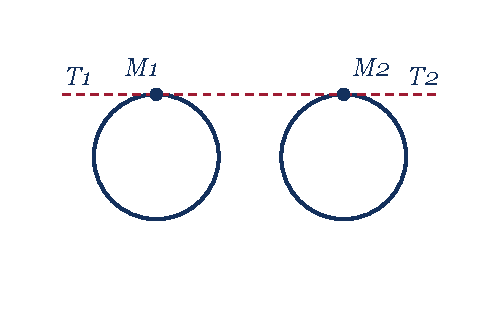
\includegraphics[width=0.7\textwidth]{figuras/pdf/cap04-fig7.pdf}
\caption{Tangentes paralelas y de igual sentido en $M_1$ y $M_2$: segunda
categoría de extremos.}
\label{fig:cap4-7}
\end{figure}

Para la segunda categoría deberá tenerse
\[
\frac{\pi}{2}v_2^2 = \frac{\pi}{2}v_1^2 + 2K\pi,
\]
siendo $\dfrac{\pi}{2}v^2$ el ángulo formado por la tangente en un punto
con el eje $x$. Esta igualdad nos da $v_2^2-v_1^2=4K$, o bien
\[
v_2+v_1 = \frac{4K}{l},
\]
poniendo $l=v_2-v_1$.

En cuanto a los máximos y mínimos de la primera categoría, su búsqueda es
muy complicada.

\section{Difracción por el borde de una pantalla}

\noindent\textbf{101. Difracción por el borde de una pantalla.} — En este
caso, el límite $v_2$ de la integral (3) del §96 es infinito y la
intensidad luminosa en un punto $P$ es proporcional al cuadrado del
módulo de
\[
\int_{v_1}^{\infty} e^{\frac{i\pi}{2}v^2}\,dv.
\]
Si $M_1$ es el punto correspondiente a $v_1$, este módulo es igual a la
longitud $AM_1$ de la recta que une el punto asintótico $A$ con el punto
$M_1$.

Cuando el punto $P$ está en el interior de la sombra geométrica, su polo
$Q$ está sobre la pantalla; por consiguiente, el límite inferior $v_1$ de
la integral precedente es positivo y el punto $M_1$ que le corresponde
está en la parte de la curva situada del mismo lado que $A$
(figura~\ref{fig:cap4-8}). La intensidad va, pues, decreciendo muy
rápidamente en cuanto nos alejamos del borde de la sombra geométrica sin
presentar ni máximo ni mínimo.

\begin{figure}[ht]
\centering
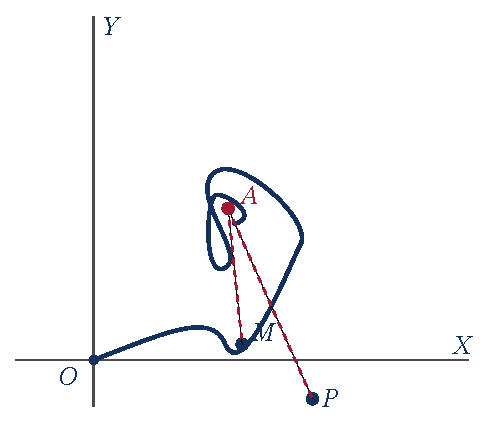
\includegraphics[width=0.6\textwidth]{figuras/pdf/cap04-fig8.pdf}
\caption{El punto asintótico $A$, el punto $M$ y la distancia $AM$ en la
sombra geométrica del borde de una pantalla.}
\label{fig:cap4-8}
\end{figure}

Siendo $AM$ aproximadamente igual a $\dfrac{1}{\pi v}$, el cuadrado del
módulo de nuestra integral es igual aproximadamente a $\dfrac{1}{\pi^2v^2}$.

Por consiguiente, del lado de la sombra geométrica, la intensidad
luminosa varía sensiblemente en razón inversa del cuadrado de la
distancia al borde de esa sombra.

Si el punto $P$ está fuera de la sombra geométrica, su polo $Q$ está
fuera de la pantalla; el valor límite $v_1$ es negativo y el punto $M_1$
está en la parte de la curva situada debajo del eje $x$. La recta $AM_1$
y, por consiguiente, la intensidad en $P$, presentarán una sucesión de
máximos y de mínimos; tendremos franjas. Los máximos y mínimos de $AM_1$
corresponden a los puntos donde esta recta es normal a la curva. Cuando
el punto $M_1$ es vecino de $A'$, las normales a la curva que pasan por
$A$ difieren poco de la recta $AA'$
(figura~\ref{fig:cap4-9}). Formando esta recta con $ox$ un ángulo igual a
$\dfrac{\pi}{4}$, la tangente en un punto correspondiente a un máximo o a
un mínimo forma con $ox$ un ángulo dado por la fórmula
\[
-\frac{\pi}{4}+K\pi.
\]

\begin{figure}[ht]
\centering
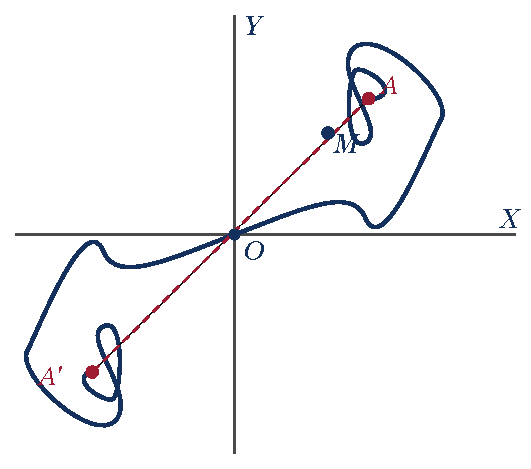
\includegraphics[width=0.6\textwidth]{figuras/pdf/cap04-fig9.pdf}
\caption{Los dos puntos asintóticos $A$, $A'$ y la recta $AA'$, que forma
un ángulo de $\pi/4$ con el eje $ox$.}
\label{fig:cap4-9}
\end{figure}

Teniendo este ángulo por valor, en función de $v$, $\dfrac{\pi}{2}v^2$,
tendremos la igualdad
\[
\frac{\pi}{2}v^2 = -\frac{\pi}{4}+K\pi,
\]
que nos dará, para $v^2$,
\[
v^2 = 2K-\frac12.
\]
Tal es la fórmula que da aproximadamente los valores de $v^2$
correspondientes a los máximos y mínimos.

Sean $M_1$ y $M_2$ dos puntos correspondientes a un máximo y a un mínimo
consecutivos. La diferencia de intensidad será
\[
AM_1^2 - AM_2^2.
\]
Si el máximo es de orden elevado, los puntos $M_1$ y $M_2$ estarán muy
próximos el uno del otro y estarán sensiblemente sobre la recta $AA'$;
tendremos entonces, sensiblemente,
\[
AM_1+AM_2 = 2AA',\qquad
AM_1-AM_2 = A'M_1+A'M_2 = \frac1{\pi v_1}+\frac1{\pi v_2},
\]
siendo $v_1$ y $v_2$ los valores de $v$ que corresponden a $M_1$ y a
$M_2$. La diferencia de intensidad será, pues,
\[
2AA'\left(\frac1{v_1}+\frac1{v_2}\right),
\]
lo que muestra que la diferencia entre un máximo y un mínimo consecutivos
varía sensiblemente en razón inversa de la distancia al borde de la
sombra geométrica.

\section{Difracción por una pequeña pantalla circular}

\noindent\textbf{102. Difracción por una pequeña pantalla circular.} —
Supongamos que una pequeña pantalla circular ocupa una parte de la esfera
$S$. Para obtener las variaciones de la intensidad luminosa en los
distintos puntos de un plano situado a una distancia $b$ del centro de la
pantalla, deberemos, como antes, estudiar las variaciones de la integral
\begin{equation}
\iint e^{\frac{i\pi}{2}(u^2+v^2)}\,du\,dv,
\tag{1}
\end{equation}
extendida a todos los puntos del plano tangente a la esfera en $Q$, que
están fuera de la pantalla.\footnote{A partir de aquí, y durante el resto
del capítulo, Poincaré reinicia la numeración de sus ecuaciones en casi
cada nueva subsección —ya ocurrió varias veces en la primera mitad del
capítulo—. Conservamos cada numeración tal como aparece en el original,
sin renumerar de forma continua.~(N.~del T.)}

Busquemos en particular la iluminación en un punto situado sobre la recta
que une la fuente luminosa con el centro de la pantalla; el polo del
punto considerado se encuentra entonces en el centro de la pantalla.
Pongamos
\[
u=\rho\cos\varphi,\qquad v=\rho\sin\varphi.
\]
Tendremos
\[
\rho^2=u^2+v^2,
\]
y, como $u$ y $v$ son proporcionales a las distancias de un punto del
plano tangente en $Q$ a dos ejes rectangulares que pasan por $Q$, $\rho$
será proporcional a la distancia de ese punto a $Q$. Por consiguiente, si
tomamos como coordenadas $\rho$ y $\varphi$, los bordes de la pantalla
tendrán para $\rho$ un valor constante $a$. El producto $du\,dv$,
proporcional a la superficie de un elemento, se convierte en este sistema
de coordenadas en $\rho\,d\rho\,d\varphi$; por consiguiente, la integral
que da la intensidad es
\begin{equation}
\int_a^\infty\int_0^{2\pi} e^{\frac{i\pi}{2}\rho^2}\,\rho\,d\rho\,d\varphi.
\tag{2}
\end{equation}
Integrando respecto de $\varphi$, se tiene
\begin{equation}
2\pi\int_a^\infty e^{\frac{i\pi}{2}\rho^2}\,\rho\,d\rho;
\tag{3}
\end{equation}
y haciendo la integración respecto de $\rho$, se obtiene
\[
2\pi\left[\frac{1}{i\pi}e^{\frac{i\pi}{2}\rho^2}\right]_a^\infty
= -2i\left[e^{\frac{i\pi}{2}\rho^2}\right]_a^\infty.
\]
Para el límite $\rho=\infty$, el valor de la exponencial imaginaria es
indeterminado. Tomaremos para este valor cero, pues nuestras fórmulas
solo se aplican al caso en que $\rho$ es pequeño, y los elementos de la
integral (3) que corresponden a valores muy grandes de $\rho$ no deben
considerarse. Tendremos, pues, simplemente,
\[
\iint e^{\frac{i\pi}{2}(u^2+v^2)}\,du\,dv = 2i\,e^{\frac{i\pi}{2}a^2}.
\]
El módulo de esta última exponencial es 2. La intensidad luminosa en el
punto considerado es, pues, independiente de $a$, y por consiguiente del
radio de la pantalla; tiene el mismo valor que si $a=0$, es decir, que si
la pantalla no existiera.

Esta consecuencia de las fórmulas de difracción fue hallada por Poisson.
Fresnel verificó experimentalmente la presencia de este punto luminoso en
el centro de la sombra geométrica dada por una pequeña pantalla circular.

\begin{notahistorica}
Este es el célebre \emph{punto de Poisson} (también llamado punto de
Arago), ya mencionado en el Capítulo III a propósito de la controversia
entre Fresnel y Poisson sobre el principio de Huygens: una predicción que
Poisson creía absurda y que Arago confirmó experimentalmente, en una de
las demostraciones más contundentes de la naturaleza ondulatoria de la
luz.
\end{notahistorica}

Se concibe fácilmente que este fenómeno no se produzca sino con una
pequeña pantalla, pues, en caso contrario, nuestras fórmulas ya no son
aplicables. En efecto, hemos visto (§95) que la intensidad en un punto
depende de los valores de $\xi_1$ y de $\dfrac{d\xi_1}{dt}$ en los
distintos puntos de la esfera $S$, valores que hemos supuesto constantes;
lo cual no puede ser cierto sino si consideramos una porción muy pequeña
de la esfera $S$.

\section{Difracción por una pequeña abertura circular}

\noindent\textbf{103. Difracción por una pequeña abertura circular.} —
En este caso, los límites de la integral (3) del párrafo precedente son
$0$ y $a$. Tenemos, pues, para la intensidad en un punto cuyo polo ocupa
el centro de la abertura, una cantidad proporcional al módulo de
\[
2i\left(1-e^{\frac{i\pi}{2}a^2}\right).
\]
El módulo del primer factor es 2, el del segundo factor varía de 0 a 2
con el valor de $a$. Este módulo es nulo para $a^2=4K$, siendo $K$ un
entero; es igual a 2 para $a^2=4K+2$. Tendremos, pues, en un mismo punto
del espacio, oscuridad o luz según el radio de la abertura. Alrededor de
ese punto, se tendrán franjas que, por razón de simetría, deberán ser
circulares.

\section{Difracción en luz paralela}

\noindent\textbf{104. Difracción en luz paralela.} — Un caso
particularmente interesante de la difracción es aquel en que se observan
los fenómenos a gran distancia de una pantalla colocada muy lejos de la
fuente luminosa. Podremos entonces considerar el radio de la esfera que
contiene la pantalla como infinito, y esta esfera se convertirá en un
plano.

Sea $P$ (figura~\ref{fig:cap4-10}) un punto del espacio; una de las
componentes del desplazamiento de este punto será la parte real de
\[
\xi = e^{-i\alpha Vt}\int X\,\frac{e^{i\alpha r}}{r}\,d\omega,
\]
siendo $X$ una función del desplazamiento $\xi_1$ de un punto del plano
$R$, y extendiéndose la integral a todos los puntos de ese plano.

\begin{figure}[ht]
\centering
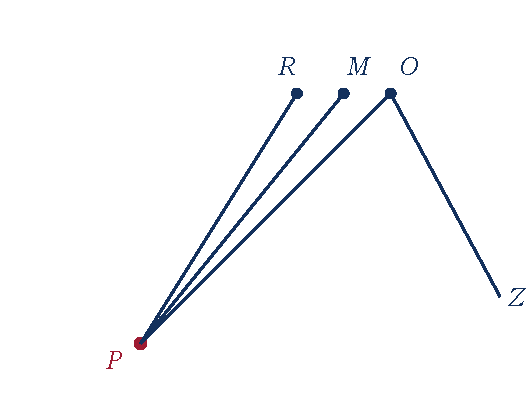
\includegraphics[width=0.75\textwidth]{figuras/pdf/cap04-fig10.pdf}
\caption{Difracción en luz paralela: el punto $P$, el plano $R$ con los
puntos $M$ y $O$ vecinos, y la dirección $OZ$.}
\label{fig:cap4-10}
\end{figure}

Hemos visto que cuando la pantalla no estaba muy alejada de la fuente
luminosa, solo la porción de la esfera vecina del polo del punto $P$
tenía influencia sobre la iluminación de ese punto. Lo mismo ocurrirá
cuando el radio de la esfera se vuelva infinito, y no tendremos que
considerar en la búsqueda de la iluminación del punto $P$ más que los
puntos del plano $R$ vecinos del pie de la perpendicular bajada de $P$
sobre el plano. Podremos, pues, suponer que la función $X$ tiene un valor
constante y sacarla del signo de integración. Además, estando el punto
$P$ supuesto alejado del plano, sus distancias $PO$ y $PM$ a dos puntos
vecinos $M$ y $O$ diferirán poco la una de la otra, y podremos considerar
el factor $\dfrac1r$ como teniendo el mismo valor para todos los
elementos de la integral que no son despreciables. Tendremos, pues, para
esta integral
\[
\int X\,\frac{e^{i\alpha r}}{r}\,d\omega = \frac{X}{r}\int e^{i\alpha r}\,d\omega
= \frac{X e^{i\alpha r_0}}{r}\int e^{i\alpha(r-r_0)}\,d\omega,
\]
llamando $r_0$ a la distancia del punto $P$ a un punto arbitrario $O$ del
plano $Q$.

\noindent\textbf{105.} Por las mismas consideraciones que las expuestas
en el §95, llegaríamos a mostrar que la intensidad luminosa de los
distintos puntos de un plano paralelo a $R$ es proporcional al cuadrado
del módulo de la integral
\begin{equation}
\int e^{i\alpha(r-r_0)}\,d\omega.
\tag{1}
\end{equation}
Transformemos esta integral. Desde el punto $M$ bajemos sobre $OP$ la
perpendicular $MM'$ y designemos por $P$ el ángulo $OPM$ y por $r$ la
distancia $PM$; tendremos
\[
PM' = r\cos P = r - r(1-\cos P) = r - 2r\sin^2\frac{P}{2}.
\]
El ángulo $P$ es muy pequeño, puesto que solo consideramos puntos del
plano $R$ vecinos los unos de los otros; por consiguiente $\sin^2\dfrac{P}{2}$
es el cuadrado de una cantidad muy pequeña, y aunque $r$ se suponga muy
grande, el producto $2r\sin^2\dfrac{P}{2}$ será despreciable. Tendremos
$PM'=r$ y $OM'=r_0-r$.

Tomemos en el plano $R$ dos ejes de coordenadas rectangulares que pasen
por $O$. Si designamos por $x$ e $y$ las coordenadas de $M$ y por $l$ y
$m$ los cosenos de la dirección $OP$ con los ejes, tendremos para $OM'$,
que es la proyección de $OM$ sobre $OP$,
\[
OM' = lx+my,
\]
y por consiguiente,
\[
r_0-r = lx+my.
\]
Llevando esta expresión de $r_0-r$ a la integral (1), se convierte en
\[
\int e^{-i\alpha(lx+my)}\,d\omega;
\]
pero, como solo tenemos que considerar el cuadrado del módulo de esta
integral, podemos tomar
\begin{equation}
\int e^{i\alpha(lx+my)}\,d\omega,
\tag{2}
\end{equation}
cuyo módulo es el mismo.

\section{Franjas producidas por una abertura con centro de simetría}

\noindent\textbf{106. Franjas producidas por una abertura con centro de
simetría.} — En general los mínimos de intensidad luminosa no son nulos,
pues el módulo de nuestra integral solo podría anularse si la parte real
y la parte imaginaria se anularan a la vez, lo que en general no ocurrirá;
pero en el caso de la difracción producida por una abertura que tiene un
centro de simetría, esos mínimos son iguales a cero.

En efecto, si suponemos que el punto $O$ es el centro de simetría de la
abertura, la integral
\[
\int e^{i\alpha(lx+my)}\,d\omega,
\]
extendida a todos los puntos de la abertura, debe conservar el mismo
valor cuando se cambia $x$ en $-x$ e $y$ en $-y$. Con este cambio la
integral se convierte en
\[
\int e^{-i\alpha(lx+my)}\,d\omega.
\]
La parte imaginaria de esta integral es de signo contrario a la parte
imaginaria de la integral precedente. Como estas dos integrales tienen el
mismo valor, la parte imaginaria es nula y cada una de ellas se reduce a
la parte real,
\[
\int \cos\alpha(lx+my)\,d\omega.
\]
Esta integral es real y no es en general siempre del mismo signo, de modo
que debe anularse; por lo tanto, en luz homogénea los mínimos de
intensidad son rigurosamente nulos.

\section{Difracción por aberturas semejantes}

\noindent\textbf{107. Difracción por aberturas semejantes.} — Designemos
por $\delta$ el ángulo de la dirección $OP$ (figura~\ref{fig:cap4-10}) con
la perpendicular en $O$ al plano de la abertura. Vamos a mostrar que si
reemplazamos esta abertura por una abertura semejante cuya razón de
similitud con la primera es $K$, el seno del ángulo de desviación
$\delta$ que corresponde a una misma franja queda dividido por $K$.

Si $x$ e $y$ son las coordenadas de un punto de la primera abertura, las
coordenadas del punto correspondiente en la abertura semejante serán
$Kx$ y $Ky$. La intensidad luminosa en un punto $P$ al que corresponden
los cosenos directores $l$ y $m$ será, en el caso de la primera abertura,
proporcional al cuadrado del módulo de
\[
\int e^{i\alpha(lx+my)}\,d\omega,
\]
y en el caso de la segunda, al cuadrado del módulo de
\[
\int e^{i\alpha K(lx+my)}\,K^2\,d\omega.
\]
Si consideramos un punto $P_1$ situado siempre a la misma distancia del
plano $R$, pero cuyos cosenos con los ejes $x$ e $y$ son $\dfrac{l}{K}$ y
$\dfrac{m}{K}$, la intensidad luminosa en ese punto será, con la segunda
abertura, proporcional al cuadrado del módulo de
\[
\int e^{i\alpha(lx+my)}\,K^2\,d\omega.
\]
Esta intensidad será proporcional a la intensidad en el punto $P$
supuesto iluminado por la rendija primitiva, y los máximos o mínimos de
estas intensidades tendrán lugar al mismo tiempo. Busquemos el seno del
ángulo de desviación $\delta_1$ del punto $P_1$. Llamando $\varphi$ al
ángulo del plano $POZ$ con el plano de los $xz$, se tiene
\[
l=\sin\delta\cos\varphi\qquad m=\sin\delta\sin\varphi.
\]
Por consiguiente
\[
\sin^2\delta = l^2+m^2.
\]
Para el punto $P_1$ tendremos
\[
\sin^2\delta_1 = \frac{l^2}{K^2}+\frac{m^2}{K^2},
\]
y por consiguiente
\[
\sin^2\delta_1 = \frac{\sin^2\delta}{K^2}.
\]

Esta igualdad nos muestra que si se reemplaza una abertura por una
segunda $K$ veces más grande, el seno del ángulo de desviación
correspondiente a una misma franja queda dividido por $K$; el plano de
difracción será, por lo demás, el mismo, puesto que la razón $\dfrac{l}{m}$
no ha variado.

Así, dos aberturas semejantes producirán figuras de difracción
semejantes; pero las dimensiones de estas figuras estarán en razón
inversa de las dimensiones de las aberturas.

\section{Teorema de Bridge}

\noindent\textbf{108. Teorema de Bridge.} —

\begin{enunciado}{Teorema de Bridge}
Cuando una pantalla está perforada por varias aberturas idénticas y
dispuestas de manera semejante, la intensidad en un punto es igual a la
intensidad resultante de una sola abertura multiplicada por la intensidad
debida a un conjunto de puntos luminosos dispuestos en el plano como lo
están las aberturas.
\end{enunciado}

La intensidad en un punto $P$ es proporcional al cuadrado del módulo de
la integral
\begin{equation}
\int e^{i\alpha(lx+my)}\,d\omega,
\tag{1}
\end{equation}
extendida a todas las porciones iluminadas de la pantalla. Esta integral
será la suma de integrales de la misma forma extendidas a la superficie
de cada una de las aberturas. Siendo estas aberturas iguales y dispuestas
de manera semejante, si a un punto de coordenadas $x$ e $y$ de una de
ellas corresponde un punto de coordenadas $x+a$ e $y+b$ de otra,
tendremos todos los puntos de esta última dando a $x$ e $y$ todos los
valores que estas cantidades pueden tomar en la primera abertura. Por
consiguiente, el término de la integral (1) que corresponde a una
abertura cualquiera es igual a
\[
\int e^{i\alpha(l(a+x)+m(b+y))}\,d\omega
= e^{i\alpha(la+mb)}\int e^{i\alpha(lx+my)}\,d\omega,
\]
estando estas integrales extendidas a toda la superficie de una de las
aberturas. La integral (1) tendrá, pues, por valor el producto
\[
\left(1+e^{i\alpha(la+mb)}+\ldots\right)\int e^{i\alpha(lx+my)}\,d\omega,
\]
que se puede escribir
\[
\sum e^{i\alpha(la+mb)}\int e^{i\alpha(lx+my)}\,d\omega,
\]
obteniéndose la unidad al hacer $a=b=0$.

El cuadrado del módulo del primer factor es proporcional a la intensidad
luminosa debida a $n$ puntos dispuestos en el plano como lo están las
aberturas de la pantalla; el cuadrado del módulo de la integral es
proporcional a la intensidad debida a una sola abertura. El teorema de
Bridge queda, pues, demostrado.

\section{Teorema de Babinet}

\noindent\textbf{109. Teorema de Babinet.} —

\begin{enunciado}{Teorema de Babinet}
Dos pantallas complementarias, es decir, tales que a los vacíos de una
corresponden los llenos de la otra, dan en un punto del espacio la misma
iluminación, excepto si ese punto está en la dirección de $oz$.
\end{enunciado}

\begin{notahistorica}
Jacques Babinet (1794-1872), físico y astrónomo francés, enunció este
principio en 1837. Es un resultado notable porque permite deducir
inmediatamente el patrón de difracción de una pantalla a partir del de su
complementaria —por ejemplo, el de un disco opaco a partir del de una
abertura circular del mismo tamaño— sin necesidad de un nuevo cálculo.
\end{notahistorica}

Designemos por $R$ la porción iluminada de la primera pantalla y por $R'$
la porción iluminada de la segunda. Como a las partes no iluminadas de la
primera pantalla corresponden las partes iluminadas de la segunda, la
suma de las superficies $R$ y $R'$ debe ser igual a todo el plano. La
intensidad luminosa en un punto del espacio será, con la primera
pantalla, proporcional al cuadrado del módulo de la integral
\[
\int e^{i\alpha(lx+my)}\,d\omega.
\]
extendida a toda la porción iluminada de la pantalla. Con la segunda
pantalla, será preciso, para obtener la intensidad, extender esta
integral a todos los puntos de la porción iluminada $R'$ de la pantalla.
La suma de estas dos integrales será la integral extendida a todo el
plano, es decir,
\[
\int_{-\infty}^{+\infty} e^{i\alpha(lx+my)}\,d\omega.
\]

El cuadrado del módulo de esta integral representa la iluminación debida
a una abertura muy grande; según lo que hemos visto a propósito de las
aberturas semejantes, los ángulos de desviación son tanto más pequeños
cuanto mayores son las dimensiones de la abertura. Para una abertura muy
grande, las desviaciones serán muy pequeñas, es decir, que no habrá luz
sensible más que en la dirección del eje de las $z$.

Esta integral es, pues, nula para todos los puntos del espacio que no son
vecinos del eje $oz$. Por consiguiente, para todos esos puntos, las
integrales que sirven para hallar la intensidad en un punto no
diferirán más que por el signo y el cuadrado de su módulo tendrá el mismo
valor. La intensidad luminosa es, pues, la misma en esos puntos.

\section{Difracción por aberturas alargadas}

\noindent\textbf{110. Difracción por aberturas alargadas.} — Supongamos
que reemplazamos la abertura de una pantalla por otra obtenida
multiplicando las ordenadas de cada punto de la primera por la misma
cantidad $K$ sin cambiar las abscisas. En tal transformación un cuadrado
se convierte en un rectángulo, un círculo se convierte en una elipse.

La intensidad luminosa en un punto del espacio cuando se toma la segunda
abertura es proporcional al cuadrado del módulo de la integral
\[
\int e^{i\alpha(lx+Kmy)}\,K\,d\omega.
\]
Por consiguiente, la intensidad luminosa dada por la segunda abertura en
un punto $P_1$ al que corresponden los cosenos $l$ y $\dfrac{m}{K}$ será
$K$ veces la intensidad dada por la primera abertura en un punto $P$ tal
que los cosenos directores de $OP$ sean $l$ y $m$.

Si en el plano que pasa por $P$ y es paralelo al plano $R$ de la
figura~\ref{fig:cap4-10}, trazamos ejes de coordenadas paralelos a los
$x$ y a los $y$ trazados en el plano $R$, las coordenadas $x_1$ e $y_1$
de $P$ respecto de estos ejes serán iguales a las coordenadas de la
proyección de ese punto sobre el plano $R$. Los cosenos directores de la
dirección $OP$ son $l$, $m$ y $\cos\delta$; por consiguiente, designando
por $z$ la distancia constante del punto $P$ al plano $R$, se tiene
\[
x_1 = \frac{lz}{\cos\delta}\qquad y_1 = \frac{mz}{\cos\delta},
\]
o, reemplazando $\cos\delta$ por su valor en función de $l$ y de $m$,
\[
x_1 = \frac{lz}{\sqrt{1-l^2-m^2}}\qquad y_1 = \frac{mz}{\sqrt{1-l^2-m^2}}.
\]

Por consiguiente, cuando se reemplaza una abertura por otra cuyas
ordenadas son $K$ veces más grandes, las coordenadas del punto cuya
intensidad es $K$ veces la que poseía el punto $x_1$, $y_1$ con la
abertura primitiva son
\[
x_1' = \frac{lz}{\sqrt{1-l^2-\dfrac{m^2}{K^2}}}\qquad
y_1' = \frac{mz}{K\sqrt{1-l^2-\dfrac{m^2}{K^2}}}.
\]
Este punto se ha, pues, acercado al eje de las $x_1$.

Las desviaciones son generalmente pequeñas, de modo que podemos
despreciar $l^2$ y $m^2$ y escribir
\[
x_1=lz,\qquad y_1=mz,\qquad x_1'=lz,\qquad y_1'=\frac{mz}{K},
\]
o bien
\[
x_1=x_1',\qquad y_1'=\frac{y_1}{K}.
\]
La abscisa del punto que corresponde a un máximo de intensidad no ha
cambiado, pues, mientras que la ordenada se ha vuelto $K$ veces más
pequeña. Se deducirán, pues, las nuevas figuras de difracción de las
antiguas multiplicando las ordenadas de todos los puntos por
$\dfrac{1}{K}$.

Supongamos en particular que la abertura primitiva sea circular. Por
razón de simetría, las franjas de difracción serán también circulares.
Si multiplicamos las ordenadas de los distintos puntos de la abertura por
$K$, esta abertura se convertirá en una elipse. Para obtener las nuevas
franjas de difracción, será necesario multiplicar las ordenadas de las
antiguas franjas por $\dfrac1K$; estas franjas se convertirán así en
elípticas.

Así, una abertura elíptica produce figuras de difracción que son también
elipses. Estas elipses son semejantes a la abertura pero inversamente
colocadas, siendo el eje mayor de las franjas elípticas paralelo al eje
menor de la abertura.

Si tomamos una rendija muy alargada, los puntos donde la intensidad es
nula estarán muy cerca del eje de las $x_1$, pues se puede considerar tal
rendija como resultante de un cuadrado cuyo lado paralelo al eje de las
$y$ se ha multiplicado por un número muy grande $K$. No se observarán,
pues, los fenómenos de difracción más que en el plano de los $xz$, es
decir, en un plano perpendicular a la longitud de la rendija.

\section{Difracción por una rendija o pantalla rectangular}

\noindent\textbf{111. Difracción por una rendija o pantalla rectangular.}
— Designemos por $2a$ y $2b$ las dimensiones de la rendija. Para obtener
la intensidad luminosa dada en un punto $P$ por esta abertura, debemos
considerar la integral
\[
\int e^{i\alpha(lx+my)}\,d\omega,
\]
extendida a toda la superficie de la rendija. El elemento de superficie
$d\omega$ siendo igual al producto $dx\,dy$, tendremos para nueva forma
de esta integral
\[
\iint e^{i\alpha(lx+my)}\,dx\,dy;
\]
y como podemos suponer que el origen de las coordenadas coincide con el
centro de la rendija, los límites de integración serán $-a$ y $+a$ para
$x$, y $-b$ y $+b$ para $y$. Siendo constantes los límites de
integración, la integral precedente es el producto de las dos integrales
simples, tomadas una respecto de $x$, y la otra respecto de $y$.
Tendremos que buscar el módulo del producto
\[
\int_{-a}^{+a} e^{i\alpha lx}\,dx \int_{-b}^{+b} e^{i\alpha my}\,dy.
\]
Para simplificar nuestras expresiones, pongamos
\begin{equation}
\alpha l=u\qquad \alpha m=v;
\tag{1}
\end{equation}
tendremos
\[
\int_{-a}^{+a} e^{iux}\,dx \int_{-b}^{+b} e^{ivy}\,dy.
\]
La primera integral de este producto tiene por valor
\[
\frac{e^{iau}-e^{-iau}}{iu} = \frac{2\sin au}{u}.
\]
El valor de la integral tomada respecto de $y$ es
\[
\frac{e^{ibv}-e^{-ibv}}{iv} = \frac{2\sin bv}{v}.
\]
El producto de las dos integrales será
\[
4\,\frac{\sin au}{u}\cdot\frac{\sin bv}{v},
\]
o también
\[
4ab\,\frac{\sin au}{au}\cdot\frac{\sin bv}{bv}.
\]
Tendremos, pues, para la intensidad luminosa, una cantidad proporcional a
\begin{equation}
\left(\frac{\sin au}{au}\right)^2 \times \left(\frac{\sin bv}{bv}\right)^2.
\tag{2}
\end{equation}
Esta intensidad se volverá nula cuando uno de los senos sea nulo, es
decir, para
\begin{equation}
au=K\pi,\qquad\text{o}\qquad bv=K'\pi,
\tag{3}
\end{equation}
donde $K$ y $K'$ son enteros cualesquiera, pero que no pueden suponerse
nulos. En efecto, para $K=0$ o $K'=0$, el valor de los dos factores
$\dfrac{\sin au}{au}$, $\dfrac{\sin bv}{bv}$ es la unidad, y por
consiguiente la intensidad no es nula; es incluso máxima, siendo la
unidad el mayor valor absoluto que puede tomar cada uno de los factores.
Observemos que si $K$ y $K'$ son nulos se tiene $u=v=0$ y por
consiguiente $l=m=0$. El punto cuya iluminación se busca está entonces
situado sobre el eje $oz$ (figura~\ref{fig:cap4-10}), es decir, sobre una
perpendicular al plano de la rendija elevada por el centro de esta
rendija. En todo punto de esta recta la intensidad es máxima.

\noindent\textbf{112.} Los valores de $l$ y de $m$ que corresponden a los
mínimos de intensidad se obtienen reemplazando en las ecuaciones de
condición (3) $u$ y $v$ por sus valores (1); estos valores son
\[
l=\frac{K\pi}{a\alpha},\qquad m=\frac{K'\pi}{b\alpha}.
\]
Hemos visto (§110) que si se toman en el plano donde se observan los
fenómenos dos ejes paralelos a los ejes $x$ y $y$ y que se cortan sobre
$oz$, las coordenadas $x_1$ e $y_1$ de un punto son proporcionales a $l$ y
a $m$. Por consiguiente, los puntos cuya intensidad es nula están
situados sobre rectas paralelas a uno de los ejes de coordenadas y
equidistantes entre sí. El fenómeno tendrá, pues, el aspecto de una serie
de mallas rectangulares luminosas, cuyo centro presenta un máximo de
iluminación. Estos máximos decrecen muy rápidamente en cuanto nos
alejamos de los ejes, es decir, en cuanto $u$ o $v$ aumenta, puesto que
la expresión (2) a la cual es proporcional la intensidad contiene en el
denominador el producto $u^2v^2$. Así, apenas se ve más que una cruz
luminosa en la dirección de los ejes, formada por los puntos que
corresponden a $K=0$ o $K'=0$.

El teorema de Babinet nos indica que se tendrá el mismo fenómeno tomando
una pequeña pantalla rectangular.

Si una de las dimensiones de la rendija tiene un tamaño considerable, no
se tendrán, según el §110, fenómenos observables más que en el plano
perpendicular a la mayor dimensión de la rendija. Se verá una serie de
bandas de intensidad nula separadas por bandas luminosas cuyo brillo
decrece muy rápidamente a partir de la banda central. El cálculo muestra
que al segundo máximo corresponde una intensidad 20 veces menor que al
primero.

Los mismos fenómenos se observarían con un hilo.

\section{Caso de \texorpdfstring{$n$}{n} puntos luminosos irregularmente
dispuestos en un plano}

\noindent\textbf{113. Caso de $n$ puntos luminosos irregularmente
dispuestos en un plano.} — Llamando $a$ y $b$ a las coordenadas de uno
cualquiera de estos puntos, que supondremos de la misma intensidad, la
intensidad luminosa en un punto del espacio es proporcional al cuadrado
del módulo de la suma
\[
\sum e^{i(ua+vb)};
\]
ahora bien, el producto de dos cantidades imaginarias conjugadas es igual
al cuadrado del módulo de una de esas imaginarias; la intensidad luminosa
será, pues, proporcional a
\[
\sum e^{i(ua+vb)} \sum e^{-i(ua+vb)} = \sum e^{i[u(a-a')+v(b-b')]},
\]
siendo $a'$ y $b'$ las coordenadas de un segundo punto luminoso
cualquiera.

El número de términos de este producto es $n^2$. Para $n$ de entre ellos,
se tiene $a=a'$, $b=b'$ y el valor de cada uno de ellos es 1; su suma
será $n$. Para los $n^2-n$ términos restantes el módulo es 1 y el
argumento $u(a-a')+v(b-b')$. Este argumento puede tomar todos los valores
posibles puesto que los puntos están distribuidos irregularmente. Ahora
bien, se sabe que el valor medio de $e^{i\varphi}$, donde $\varphi$ puede
tomar todos los valores posibles, es cero; por consiguiente, la suma de
los $n^2-n$ términos considerados es nula. La intensidad en un punto
iluminado por los $n$ puntos de igual intensidad será, pues, una
constante igual a $n$ veces la intensidad dada por un solo punto
iluminante.

\section{Caso de \texorpdfstring{$n$}{n} aberturas}

\noindent\textbf{114. Caso de $n$ aberturas.} — Consideremos $n$ aberturas
iguales, dispuestas de manera semejante pero colocadas irregularmente en
el plano. Según el teorema de Bridge (§108), la intensidad será el
producto de dos factores, uno proporcional a la intensidad dada por una
sola rendija, y el otro proporcional a la intensidad dada por $n$ puntos
colocados en el plano como lo están las aberturas. Cuando estas aberturas
estén dispuestas irregularmente, este segundo factor será, según el
párrafo precedente, igual a $n$ veces la intensidad resultante de una
sola abertura.

El teorema de Babinet nos enseña que ocurriría lo mismo con $n$ pantallas.
En particular con $n$ pequeñas pantallas circulares se deberán tener los
mismos fenómenos que con una sola pantalla; los máximos de la intensidad
luminosa serán solamente $n$ veces más grandes. Se puede verificar este
hecho experimentalmente espolvoreando de licopodio el objetivo de un
anteojo astronómico; se perciben franjas negras y brillantes cuando se
hace la experiencia en luz homogénea.

\section{Caso de dos puntos de igual intensidad}

\noindent\textbf{115. Caso de dos puntos de igual intensidad.} — Tomemos
por eje de las $x$ una recta que pase por estos puntos, y por eje de las
$y$ una perpendicular trazada por el medio de la distancia que separa los
dos puntos. Las coordenadas de uno de los puntos serán $a$ y $0$, las del
otro, $-a$ y $0$. La intensidad luminosa en un punto del espacio será
proporcional al cuadrado del módulo de
\[
e^{iau}+e^{-iau}.
\]
Siendo esta suma igual a $2\cos au$,\footnote{El original imprime
$e^{iau}-e^{-iau}$ y dice «cette différence»; es una errata evidente por
$e^{iau}+e^{-iau}$, que es la suma que corresponde a dos puntos de igual
intensidad y vale $2\cos au$; la diferencia escrita valdría
$2i\sin au$.~(N.~del T.)} la intensidad es proporcional
a $\cos^2 au$. Los mínimos de intensidad tendrán lugar para
\[
u = \frac{(2K+1)\pi}{2a};
\]
estarán regularmente espaciados y su valor será nulo. Son debidos a la
interferencia de los rayos. Los máximos estarán regularmente espaciados e
iguales entre sí; corresponden a
\[
u = \frac{K\pi}{a}.
\]

\section{Caso de dos aberturas o de dos pantallas circulares}

\noindent\textbf{116. Caso de dos aberturas o de dos pantallas
circulares.} — Designando por $I$ la intensidad luminosa en un punto
cuando se tiene una sola abertura, y por $2a$ la distancia de los centros
de las dos aberturas, la intensidad dada por las dos aberturas será
proporcional a
\[
I\cos^2 au.
\]
Las variaciones del primer factor determinarán un sistema de franjas
concéntricas; las variaciones del segundo darán lugar a franjas
rectilíneas.

\section{Caso de dos rendijas rectangulares}

\noindent\textbf{117. Caso de dos rendijas rectangulares.} — Según el
§111, la intensidad resultante de una rendija de ancho $2b$ y cuya altura
es relativamente grande es proporcional a
\[
\left(\frac{\sin bu}{bu}\right)^2.
\]
Por consiguiente, para dos rendijas iguales distantes $2a$, tendremos
\[
\left(\frac{\sin bu}{bu}\right)^2 \cos^2 au.
\]
Los mínimos de intensidad, que serán nulos, tendrán lugar para
\[
u=\frac{K\pi}{b},\qquad u=\frac{(2K+1)\pi}{2a}.
\]
A los valores de $u$ dados por la primera igualdad corresponden franjas
de difracción, a los valores dados por la segunda corresponden franjas de
interferencia. Como $a$ es mayor que $b$, las franjas de interferencia
están más próximas entre sí que las franjas de difracción, y entre dos de
estas últimas siempre se encontrará cierto número de las primeras.

\section{Caso de \texorpdfstring{$n$}{n} puntos en línea recta y
equidistantes}

\noindent\textbf{118. Caso de $n$ puntos en línea recta y equidistantes.}
— Designemos por $2a$ la distancia de dos puntos consecutivos; tomemos
por eje de las $x$ la recta que pasa por todos los puntos y por origen el
primero de los puntos. Las abscisas serán
\[
0,\quad 2a,\quad 4a,\quad\ldots,\quad 2(n-1)a,
\]
y la integral cuyo cuadrado del módulo es proporcional a la intensidad se
convertirá en
\begin{equation}
1+e^{2iau}+e^{4iau}+\cdots+e^{2(n-1)iau}.
\tag{1}
\end{equation}
Los términos de esta suma forman una progresión geométrica cuya razón es
$e^{2iau}$; el valor de esta suma es, pues,
\[
\frac{e^{2niau}-1}{e^{2iau}-1}.
\]
No cambiaremos el módulo de esta fracción si la multiplicamos o la
dividimos por cantidades cuyo módulo es la unidad. Multipliquemos el
numerador por $e^{-niau}$ y el denominador por $e^{-iau}$; obtendremos
\[
\frac{e^{niau}-e^{-niau}}{e^{iau}-e^{-iau}},
\]
expresión que se puede escribir
\[
\frac{\sin nau}{\sin au}.
\]
La intensidad en un punto será proporcional al cuadrado de esta cantidad:
\begin{equation}
\frac{\sin^2 nau}{\sin^2 au}.
\tag{2}
\end{equation}

Estudiemos esta función. Es periódica, pues si aumentamos $u$ en
$\dfrac{\pi}{a}$, $au$ aumenta en $\pi$ y $nau$ en $n\pi$; por lo tanto el
valor absoluto de los senos no cambia.

Para los valores de $u$ dados por
\[
u=\frac{K\pi}{na},
\]
el numerador se anula y la función misma se vuelve nula, a menos que el
denominador no se anule al mismo tiempo que el numerador, lo que ocurre
para los valores de $K$ que son múltiplos de $n$. Para obtener el valor
que toma la función para los valores de $K$ múltiplos de $n$, nos basta,
puesto que la función es periódica, buscar qué se vuelve cuando se hace
$K=0$; se tiene en este caso
\[
\frac{\sin^2 nau}{\sin^2 au} = \frac{n^2a^2u^2}{a^2u^2} = n^2.
\]
La intensidad es proporcional a $n^2$; es un máximo absoluto de esta
intensidad, pues cada término de la suma (1) teniendo por módulo una
cantidad a lo sumo igual a 1, el módulo de la suma es a lo sumo igual a
$n$ y por consiguiente la intensidad tiene por valor máximo una cantidad
proporcional a $n^2$. Llamaremos máximos principales a los que
corresponden a una intensidad proporcional a $n^2$.

Entre dos de estos máximos la función (2) se anula $n-1$ veces, y entre
dos ceros consecutivos pasa por un máximo al menos; tendremos, pues, al
menos $n-2$ máximos secundarios. No puede además haber más, pues la
función es un polinomio entero de grado $n-1$ en $\cos au$; su derivada
respecto de $\cos au$ será de grado $n-2$ y no tendrá más que $n-2$
raíces, a cada una de las cuales corresponde un máximo o un mínimo.

Los máximos secundarios son muy pequeños y tanto menos aparentes cuanto
mayor es $n$. En efecto, se tiene
\[
\frac{\sin^2 nau}{\sin^2 au} < \frac{1}{\sin^2 au}.
\]
Si $\sin au$ tiene un valor finito, el segundo miembro de la desigualdad,
y por consiguiente el primero, son muy pequeños respecto de $n^2$.

Cuando $\sin au$ es pequeño, es decir, para los valores de $u$ vecinos de
$\dfrac{K\pi}{a}$, los máximos secundarios que están entonces vecinos de
los máximos principales son todavía difícilmente observables. En este
caso, estando $au$ vecino de $K\pi$, podemos, a causa de la periodicidad
de la función, suponer $au$ muy poco diferente de cero, y reemplazar
$\sin au$ por el arco; tendremos para el factor de intensidad
\[
\frac{\sin^2 nau}{a^2u^2}.
\]
El cálculo de este factor mostraría que el primer máximo secundario es 20
veces más pequeño que el máximo principal y el segundo, 60 veces más
pequeño.

\section{Redes de difracción}

\noindent\textbf{119. Redes.} — En una red tenemos $n$ rendijas de igual
ancho $2b$, paralelas y colocadas a una distancia $2a$ unas de otras. El
factor de intensidad de una sola rendija siendo
\begin{equation}
\frac{\sin^2 bu}{b^2u^2},
\tag{1}
\end{equation}
el de $n$ puntos equidistantes,
\begin{equation}
\frac{\sin^2 nau}{\sin^2 au},
\tag{2}
\end{equation}
la intensidad dada por la red será proporcional al producto de estos dos
factores. Como las rendijas tienen una altura grande respecto de su
ancho, solo se observarán franjas en un plano perpendicular a la longitud
de las rendijas.

Deberíamos, pues, observar los máximos debidos a los dos factores, pero
como $n$ es generalmente muy grande, solo serán visibles los máximos
principales debidos al factor (2). Para estos máximos, se tiene
\[
u=\frac{K\pi}{a},
\]
y la intensidad es proporcional a
\begin{equation}
n^2\,\dfrac{\sin^2\dfrac{Kb\pi}{a}}{\dfrac{K^2\pi^2b^2}{a^2}}.
\tag{3}
\end{equation}
Esta cantidad, conteniendo $K^2$ en el denominador, los máximos
principales disminuirán de intensidad a medida que nos alejemos de la
normal al plano de la red.

Si $\dfrac{b}{a}$ es muy pequeño, el producto $K\dfrac{b}{a}$ será menor
que $\dfrac12$ para un gran número de valores de $K$. En este caso el
numerador de (3) irá constantemente decreciendo y, como no se pueden
observar más de 6 o 7 máximos principales, irán decreciendo de
intensidad.

Cuando $\dfrac{b}{a}$ no es muy pequeño, el producto $K\dfrac{b}{a}$
puede volverse mayor que $\dfrac12$ para valores de $K$ inferiores a 7, y
entonces los máximos principales no decrecen regularmente, oscilando el
numerador de (3) entre 0 y 1.

Si el cociente $\dfrac{b}{a}$ es conmensurable, existe un valor de $K$
que anula $\sin\dfrac{Kb\pi}{a}$; por consiguiente, faltará el máximo
principal correspondiente. Así, si $\dfrac{b}{a}=\dfrac12$, faltarán
todos los máximos principales de orden par. En este caso particular,
$\sin\dfrac{Kb\pi}{a}$ tiene por valor absoluto la unidad cuando $K$ es un
número impar. Los máximos principales de orden impar serán
proporcionales a $\dfrac{1}{K^2}$; irán decreciendo regularmente.

Observemos que el intervalo lleno que separa dos rendijas es igual a
$2a-2b$; si, pues, cambiamos $2b$ en $2a-2b$, es decir, $b$ en $a-b$, en
nuestras fórmulas de intensidad, tendremos la intensidad resultante de
una nueva red que no difiere de la primera sino en que los espacios
opacos reemplazan a las rendijas y recíprocamente. Cambiando $b$ en
$a-b$ en $\sin\dfrac{Kb\pi}{a}$, obtenemos
\[
\sin\frac{K(a-b)\pi}{a} = \sin\left(K\pi-\frac{Kb\pi}{a}\right)
= \pm\sin\frac{Kb\pi}{a}.
\]
Por consiguiente, la fórmula (3) se convierte en
\[
n^2\,\dfrac{\sin^2\dfrac{bK\pi}{a}}{\dfrac{K^2\pi^2(a-b)^2}{a^2}}.
\]
Tendremos, pues, la misma ley de decrecimiento para los máximos
principales; resultado conforme al teorema de Babinet.

\section{Fenómenos de difracción en luz blanca}

\noindent\textbf{120. Fenómenos de difracción en luz blanca.} — En
nuestro estudio, siempre hemos supuesto $\lambda$ constante, es decir,
que suponíamos la luz homogénea. Si operamos con luz blanca, la posición
de los máximos de intensidad dependerá de $\lambda$; tendremos, pues,
franjas coloreadas. En particular, en el caso de las redes, siendo la
desviación muy considerable, tendremos espectros completos separados por
intervalos oscuros.


% ============================================================
% Capítulo V — Polarización rotatoria. Dispersión
% Traducción de "Théorie mathématique de la lumière" (1889), cap. V
% Original: §§121-143, páginas impresas 176-216 (PDF 192-232)
% ============================================================
\chapter{Polarización rotatoria. Dispersión}
\label{cap:polarizacion-dispersion}

\noindent\textbf{121.} Para hallar las ecuaciones
\begin{equation}
-\rho\frac{d^2\xi}{dt^2}=\sum\frac{d}{dx}\cdot\frac{d\mathrm{W}_2}{d\xi'_x},\qquad
-\rho\frac{d^2\eta}{dt^2}=\sum\frac{d}{dx}\cdot\frac{d\mathrm{W}_2}{d\eta'_x},\qquad
-\rho\frac{d^2\zeta}{dt^2}=\sum\frac{d}{dx}\cdot\frac{d\mathrm{W}_2}{d\zeta'_x}
\tag{1}
\end{equation}
del movimiento de una molécula en un medio elástico (§32), admitimos (§14)
que las cantidades $\mathrm{D}x,\mathrm{D}y,\mathrm{D}z$ eran del orden del radio de actividad
molecular, por lo que podíamos, en las expresiones de $\mathrm{D}\xi,\mathrm{D}\eta,\mathrm{D}\zeta$,
despreciar los términos que contienen $\mathrm{D}x^2,\mathrm{D}y^2,\mathrm{D}z^2$. De ello resultaba
que $\mathrm{D}\xi,\mathrm{D}\eta,\mathrm{D}\zeta$ eran funciones lineales de las nueve derivadas
parciales de $\xi,\eta,\zeta$ respecto de las variables $x,y,z$, y que
$\mathrm{W}_2$ era una función homogénea y de segundo orden respecto de esas nueve
derivadas.

Buscamos luego (§41) en qué se convertían las ecuaciones (1) en el caso de
los medios isótropos, y vimos (§42) que el movimiento de las moléculas en
ese medio se propagaba con una velocidad constante
$V=\sqrt{-2\mu/\rho}$.

Ahora bien, la experiencia demuestra que, cuando la luz atraviesa un medio
isótropo distinto del éter en el vacío, su velocidad depende de su longitud
de onda $\lambda$; nos vemos, pues, conducidos a pensar que la hipótesis
del §14, que no está justificada por ninguna consideración teórica, debe
rechazarse cuando consideramos la propagación de la luz en un medio
ponderable. Si abandonamos esta hipótesis, las cantidades $\mathrm{D}\xi,\mathrm{D}\eta,\mathrm{D}\zeta$
contendrán las derivadas de los diversos órdenes de $\xi,\eta,\zeta$
respecto de $x,y,z$, y, por consiguiente, la función $\mathrm{W}_2$, que es
homogénea y de segundo grado (§13) en $\mathrm{D}\xi,\mathrm{D}\eta,\mathrm{D}\zeta$, será homogénea y
de segundo grado respecto de las derivadas parciales de los diversos
órdenes de $\xi,\eta,\zeta$. Vamos a mostrar que las ecuaciones del
movimiento de una molécula, tomando para $\mathrm{W}_2$ una función de esta clase,
explican el fenómeno de la dispersión y el de la polarización rotatoria.

\noindent\textbf{122.} Designando por $\mathrm{U}$ la función de fuerzas relativa a
las fuerzas exteriores e interiores que se ejercen sobre las moléculas de
un volumen $R$ limitado por una superficie $S$ (figura~\ref{fig:cap5-1}),
hallamos (§29),\footnote{El original remite aquí al §27; la ecuación que
sigue, obtenida por el principio de d'Alembert y el de las velocidades
virtuales, es la (33) del §29.~(N.~del T.)} por la aplicación del principio de
d'Alembert y del principio de las velocidades virtuales, la ecuación
\begin{equation}
\delta \mathrm{U} - \int \rho\,d\tau\left(\frac{d^2\xi}{dt^2}\delta\xi
+\frac{d^2\eta}{dt^2}\delta\eta+\frac{d^2\zeta}{dt^2}\delta\zeta\right)=0,
\tag{2}
\end{equation}
que debe satisfacerse cualesquiera que sean $\delta\xi,\delta\eta,\delta\zeta$.

\begin{figure}[ht]
\centering
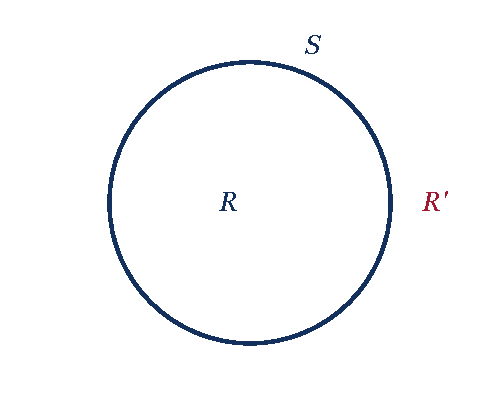
\includegraphics[width=0.45\textwidth]{figuras/pdf/cap05-fig1.pdf}
\caption{Superficie $S$ que limita un volumen $R$, con el medio exterior
$R'$.}
\label{fig:cap5-1}
\end{figure}

La parte de la función $\mathrm{U}$ que corresponde a las fuerzas interiores es
$\int \delta \mathrm{W}\,d\tau$, y la relativa a las fuerzas exteriores que se
ejercen sobre la superficie de separación $S$ es
$\int(\mathrm P_x\delta\xi+\mathrm P_y\delta\eta+\mathrm P_z\delta\zeta)\,d\omega$,
designando $\mathrm P_x,\mathrm P_y,\mathrm P_z$ las componentes, según los
tres ejes, de la presión que se ejerce sobre el elemento de superficie
$d\omega$. Sustituyendo $\delta \mathrm{U}$ por la suma de estas dos cantidades, la
ecuación (2) se convierte en
\[
\int(\mathrm P_x\delta\xi+\mathrm P_y\delta\eta+\mathrm P_z\delta\zeta)\,d\omega
+\int\delta \mathrm{W}\,d\tau
-\int\rho\,d\tau\left(\frac{d^2\xi}{dt^2}\delta\xi+\frac{d^2\eta}{dt^2}\delta\eta
+\frac{d^2\zeta}{dt^2}\delta\zeta\right)=0.
\]
Como esta ecuación debe satisfacerse cualesquiera que sean
$\delta\xi,\delta\eta,\delta\zeta$, podemos, en particular, suponer
$\delta\eta=\delta\zeta=0$, y tenemos la igualdad
\begin{equation}
\int \mathrm P_x\delta\xi\,d\omega + \int\delta \mathrm{W}\,d\tau
-\int\frac{d^2\xi}{dt^2}\delta\xi\,\rho\,d\tau=0,
\tag{3}
\end{equation}
que deberá cumplirse cualquiera que sea $\delta\xi$.

\noindent\textbf{123.} Se trata de transformar el segundo término de esta
igualdad. La función $\mathrm{W}$ es, en general, una función de las derivadas
parciales de los diversos órdenes de $\xi,\eta,\zeta$. En un desplazamiento
virtual cualquiera dado al sistema, cada una de estas derivadas varía,
pero, en el caso en que se tiene, como hemos supuesto, $\delta\eta=\delta\zeta=0$,
solo cambian de valor las derivadas parciales de $\xi$. Por consiguiente,
el incremento $\delta \mathrm{W}$ de la función $\mathrm{W}$ dependerá únicamente de los
incrementos de las distintas derivadas parciales de $\xi$. Con el fin de
simplificar los cálculos, admitiremos que las únicas derivadas parciales de
$\xi$ que entran en $\mathrm{W}$ son $d\xi/dx$ y $d^2\xi/dx^2$, derivadas que
podremos representar sin ambigüedad por $\xi'$ y $\xi''$. Tenemos
entonces,
\[
\delta \mathrm{W} = \frac{d\mathrm{W}}{d\xi'}\delta\xi' + \frac{d\mathrm{W}}{d\xi''}\delta\xi'',
\]
y, por consiguiente,
\[
\int\delta \mathrm{W}\,d\tau = \int\frac{d\mathrm{W}}{d\xi'}\delta\xi'\,d\tau
+\int\frac{d\mathrm{W}}{d\xi''}\delta\xi''\,d\tau.
\]
Se sabe, y recordamos esta propiedad en el §30, que se tiene
\begin{equation}
\int\frac{d\mathrm{W}}{d\xi'}\delta\xi'\,d\tau
=\int\alpha\frac{d\mathrm{W}}{d\xi'}\delta\xi\,d\omega
-\int\delta\xi\,\frac{d}{dx}\cdot\frac{d\mathrm{W}}{d\xi'}\,d\tau,
\tag{4}
\end{equation}
y
\[
\int\frac{d\mathrm{W}}{d\xi''}\delta\xi''\,d\tau
=\int\alpha\frac{d\mathrm{W}}{d\xi''}\delta\xi'\,d\omega
-\int\delta\xi'\,\frac{d}{dx}\cdot\frac{d\mathrm{W}}{d\xi''}\,d\tau.
\]
Esta última igualdad se convierte, al hacer sufrir a la segunda integral
del segundo miembro una transformación análoga, en
\begin{equation}
\int\frac{d\mathrm{W}}{d\xi''}\delta\xi''\,d\tau
=\int\alpha\frac{d\mathrm{W}}{d\xi''}\delta\xi'\,d\omega
-\int\alpha\delta\xi\,\frac{d}{dx}\cdot\frac{d\mathrm{W}}{d\xi''}\,d\omega
+\int\delta\xi\,\frac{d^2}{dx^2}\cdot\frac{d\mathrm{W}}{d\xi''}\,d\tau.
\tag{5}
\end{equation}
Sumando los segundos miembros de las igualdades (4) y (5), y sustituyendo
en (3) la segunda integral por esta suma, obtenemos una igualdad que
contiene integrales extendidas a la superficie $S$ e integrales extendidas
al volumen $R$. Representando la suma de las integrales dobles por $I$, la
ecuación (3) se convierte en
\[
I - \int\left(\frac{d}{dx}\cdot\frac{d\mathrm{W}}{d\xi'}
-\frac{d^2}{dx^2}\cdot\frac{d\mathrm{W}}{d\xi''}+\rho\frac{d^2\xi}{dt^2}\right)\delta\xi\,d\tau=0,
\]
y, como debe satisfacerse cualquiera que sea $\delta\xi$, el elemento
diferencial colocado bajo el signo de integración extendido al volumen debe
ser nulo. Tendremos, pues,
\[
\rho\frac{d^2\xi}{dt^2} = -\frac{d}{dx}\cdot\frac{d\mathrm{W}}{d\xi'}
+\frac{d^2}{dx^2}\cdot\frac{d\mathrm{W}}{d\xi''}.
\]
Esta ecuación se convierte, designando por $\mathrm{W}_1$ el término de primer
grado y por $\mathrm{W}_2$ el término de segundo grado en el desarrollo de $\mathrm{W}$
según las potencias crecientes de $\mathrm{D}\xi,\mathrm{D}\eta,\mathrm{D}\zeta$, en
\[
\rho\frac{d^2\xi}{dt^2} = -\frac{d}{dx}\cdot\frac{d\mathrm{W}_1}{d\xi'}
+\frac{d^2}{dx^2}\cdot\frac{d\mathrm{W}_1}{d\xi''}
-\frac{d}{dx}\cdot\frac{d\mathrm{W}_2}{d\xi'}+\frac{d^2}{dx^2}\cdot\frac{d\mathrm{W}_2}{d\xi''}.
\]
Pero, siendo $\mathrm{D}\xi,\mathrm{D}\eta,\mathrm{D}\zeta$ de primer grado (§14) respecto de las
derivadas parciales de $\xi,\eta,\zeta$, lo mismo ocurrirá con $\mathrm{W}_1$; las
derivadas de esta función respecto de $\xi'$ y $\xi''$ serán constantes, y
la ecuación anterior se reduce a
\[
\rho\frac{d^2\xi}{dt^2} = -\frac{d}{dx}\cdot\frac{d\mathrm{W}_2}{d\xi'}
+\frac{d^2}{dx^2}\cdot\frac{d\mathrm{W}_2}{d\xi''}.
\]
Esta es la primera de las ecuaciones del movimiento de una molécula; las
otras dos se obtendrían de la misma manera.

En cuanto a la suma de integrales que hemos designado por $I$, nos daría el
valor de las presiones que se ejercen sobre la superficie $S$. No
buscaremos esas presiones.

\section{Ecuaciones del movimiento}

\noindent\textbf{124. Ecuaciones del movimiento.} — Nos vemos así
conducidos a la siguiente regla. Las ecuaciones del movimiento se escribirán
\[
\rho\frac{d^2\xi}{dt^2}=\mathrm P,\qquad
\rho\frac{d^2\eta}{dt^2}=\mathrm Q,\qquad
\rho\frac{d^2\zeta}{dt^2}=\mathrm R,
\]
siendo $\mathrm P,\mathrm Q,\mathrm R$ polinomios lineales respecto de las
derivadas de los diversos órdenes de $\xi,\eta,\zeta$, y formados de la
manera siguiente:

Para formar $\mathrm P$, se diferenciará $\mathrm{W}_2$ respecto de cada una de las
derivadas parciales de $\xi$ que figuran en ella. Se diferenciará la
derivada de $\mathrm{W}_2$ así obtenida, respecto de $x$, $y$ y $z$, de la misma
manera que se hizo con la derivada parcial de $\xi$ que figura en ella. Por
ejemplo, se diferenciará
\begin{gather*}
\frac{d\mathrm{W}_2}{d\xi'_x}\ \text{una vez respecto de }x,\qquad
\frac{d\mathrm{W}_2}{d\xi''_{xx}}\ \text{dos veces respecto de }x,\\
\frac{d\mathrm{W}_2}{d\xi''_{xy}}\ \text{una vez respecto de }x\text{ y una respecto de }y,\ \text{etc.}
\end{gather*}
Se sumarán luego todas las derivadas así obtenidas, tras haber afectado del
signo $+$ las derivadas de orden par y del signo $-$ las derivadas de orden
impar. Tendremos, pues,
\begin{multline*}
\mathrm P = -\frac{d}{dx}\frac{d\mathrm{W}_2}{d\xi'_x}-\frac{d}{dy}\frac{d\mathrm{W}_2}{d\xi'_y}
-\frac{d}{dz}\frac{d\mathrm{W}_2}{d\xi'_z}\\
+\frac{d^2}{dx^2}\frac{d\mathrm{W}_2}{d\xi''_{xx}}+\cdots
+\frac{d^2}{dxdy}\frac{d\mathrm{W}_2}{d\xi''_{xy}}+\cdots
-\frac{d^3}{dx^3}\frac{d\mathrm{W}_2}{d\xi'''_{xxx}}-\cdots
\end{multline*}

Se formaría el polinomio $\mathrm Q$ de la misma manera, diferenciando
$\mathrm{W}_2$ respecto de las derivadas parciales de $\eta$.

En algunos casos particulares, la expresión del polinomio $\mathrm P$ se
simplifica. Así, si el medio elástico es isótropo, las derivadas de orden
impar no entran en $\mathrm P$. En efecto, en tal medio, las ecuaciones del
movimiento no deben cambiar cuando se cambian a la vez los signos de
$x,y,z,\xi,\eta,\zeta$. Ahora bien, al hacer este cambio, $d^2\xi/dt^2$
cambia de signo; por consiguiente, los distintos términos de $\mathrm P$
deben cambiar también de signo. Esto ocurre para todas las derivadas de
orden par respecto de $x,y,z$, pero las derivadas de orden impar, como
$d^3\xi/dx^3$, $d^3\xi/(dx^2dy)$, conservan el mismo valor puesto que sus
numeradores y sus denominadores cambian de signo al mismo tiempo. Estas
derivadas no podrán, pues, entrar en la expresión del polinomio $\mathrm P$
relativo a un medio isótropo.

Cuando el medio elástico tiene un centro de simetría, las ecuaciones del
movimiento no deben cambiar cuando se cambian los signos de
$x,y,z,\xi,\eta,\zeta$. También en este caso, el polinomio $\mathrm P$ no
deberá contener más que derivadas de orden par.

\section{Polarización rotatoria del cuarzo}

\noindent\textbf{125. Polarización rotatoria del cuarzo.} — Puesto que el cuarzo cristaliza bajo una forma
hemiédrica del sistema romboédrico, los cristales de cuarzo no poseen
centro de simetría.

Si admitimos que la distribución del éter luminoso en un cuerpo ponderable
es idéntica a la de las moléculas materiales que constituyen el cuerpo, el
éter contenido en el cuarzo será un medio elástico desprovisto de centro de
simetría.

Por consiguiente, el polinomio $\mathrm P$ que entra en las ecuaciones del
movimiento de las moléculas de éter que propagan la luz en el cuarzo podrá
contener derivadas parciales de $\xi,\eta,\zeta$ de orden impar. Vamos a
mostrar, colocándonos en condiciones particulares para evitar cálculos
demasiado largos, que la presencia de las derivadas de tercer orden basta
para dar cuenta de los fenómenos de polarización rotatoria que presenta el
cuarzo.

Consideremos una onda cuyo plano sea perpendicular al eje del cristal.
Tomando para plano de las $xy$ un plano paralelo al de la onda, los
desplazamientos $\xi,\eta,\zeta$ de las moléculas de éter no dependerán más
que de $z$ y del tiempo $t$, y, por consiguiente, las derivadas parciales
de los diversos órdenes de $\xi,\eta,\zeta$ respecto de $x$ y de $y$ serán
nulas. Además, como las vibraciones son transversales, la condición de
transversalidad, $\Theta=0$, exige que se tenga idénticamente $\zeta'_z=0$.
Por consiguiente, $\mathrm{W}_2$ será una función homogénea y de segundo grado de
las derivadas parciales de primer orden $\xi'_z,\eta'_z$ y de las derivadas
parciales de órdenes superiores de $\xi,\eta,\zeta$ respecto de $z$.
Designemos por $\mathrm{W}_2^1$ el conjunto de los términos de $\mathrm{W}_2$ que son
homogéneos respecto de las derivadas parciales de primer orden y, para
simplificar\footnote{Véase más adelante el capítulo relativo a la doble
refracción en los medios hemiédricos, donde volvemos sobre esta cuestión
con más detalle.~(N.~del T.)}, supongamos que los demás términos de $\mathrm{W}_2$ sean nulos,
con excepción del siguiente:
\[
a\,\frac{d\eta}{dz}\,\frac{d^2\xi}{dz^2}.
\]

Aplicando la regla que dimos (§124) para la formación de los segundos
miembros de las ecuaciones del movimiento, obtenemos para esas ecuaciones:
\[
\rho\frac{d^2\xi}{dt^2}=-\sum\frac{d}{dx}\frac{d\mathrm{W}_2^1}{d\xi'_x}+a\frac{d^3\eta}{dz^3},
\qquad
\rho\frac{d^2\eta}{dt^2}=-\sum\frac{d}{dx}\frac{d\mathrm{W}_2^1}{d\eta'_x}-a\frac{d^3\xi}{dz^3}.
\]

Los términos de los segundos miembros provenientes de $\mathrm{W}_2^1$ serán las
derivadas parciales de segundo orden de $\xi,\eta,\zeta$, multiplicadas por
un coeficiente constante. Admitamos que, en la primera ecuación, estos
términos se reducen a $d^2\xi/dz^2$ y que, en la segunda, se reducen a
$d^2\eta/dz^2$; tendremos entonces, para las ecuaciones del movimiento:
\begin{equation}
\rho\frac{d^2\xi}{dt^2}=\frac{d^2\xi}{dz^2}+a\frac{d^3\eta}{dz^3},
\tag{1}
\end{equation}
\begin{equation}
\rho\frac{d^2\eta}{dt^2}=\frac{d^2\eta}{dz^2}-a\frac{d^3\xi}{dz^3}.
\tag{2}
\end{equation}

Busquemos satisfacer estas ecuaciones\footnote{A
partir de aquí, el original reinicia con frecuencia su numeración local de
ecuaciones varias veces dentro de este mismo capítulo (como ya ocurrió en
los capítulos II y IV); conservamos fielmente la numeración de Poincaré en
cada caso, sin forzar una numeración continua.~(N.~del T.)} poniendo
\[
\xi=\mathrm Ae^{\frac{2i\pi}{\lambda}(z-Vt)},\qquad
\eta=\mathrm Be^{\frac{2i\pi}{\lambda}(z-Vt)}.
\]
Las derivadas parciales de $\xi$ y $\eta$ que entran en las ecuaciones del
movimiento tendrán por valor
\[
\frac{d^2\xi}{dt^2}=\mathrm A\left(\frac{2i\pi}{\lambda}\right)^2\mathrm V^2
e^{\frac{2i\pi}{\lambda}(z-Vt)},\qquad
\frac{d^2\eta}{dt^2}=\mathrm B\left(\frac{2i\pi}{\lambda}\right)^2\mathrm V^2
e^{\frac{2i\pi}{\lambda}(z-Vt)},
\]
\[
\frac{d^2\xi}{dz^2}=\mathrm A\left(\frac{2i\pi}{\lambda}\right)^2
e^{\frac{2i\pi}{\lambda}(z-Vt)},\qquad
\frac{d^2\eta}{dz^2}=\mathrm B\left(\frac{2i\pi}{\lambda}\right)^2
e^{\frac{2i\pi}{\lambda}(z-Vt)}.
\]
Llevando estos valores a las ecuaciones (1) y (2), y suprimiendo los
factores comunes a ambos miembros, obtenemos,
\begin{equation}
\mathrm A(\rho\mathrm V^2-1)=a\mathrm B\,\frac{2i\pi}{\lambda},
\tag{3}
\end{equation}
\begin{equation}
\mathrm B(\rho\mathrm V^2-1)=-a\mathrm A\,\frac{2i\pi}{\lambda}.
\tag{4}
\end{equation}
Dividiendo estas ecuaciones miembro a miembro tendremos,
\[
\frac{\mathrm A}{\mathrm B}=-\frac{\mathrm B}{\mathrm A};
\]
igualdad que puede ponerse en la forma
\[
\mathrm A^2=-\mathrm B^2,
\]
de donde
\[
\mathrm A=\pm \mathrm Bi.
\]
Podremos, pues, satisfacer las ecuaciones del movimiento tomando para
$\xi$ y $\eta$ las partes reales de
\[
\xi_1=\mathrm Bi\,e^{\frac{2i\pi}{\lambda}(z-Vt)},\qquad
\eta_1=\mathrm Be^{\frac{2i\pi}{\lambda}(z-Vt)},
\]
o de
\[
\xi_2=-\mathrm Bi\,e^{\frac{2i\pi}{\lambda}(z-Vt)},\qquad
\eta_2=\mathrm Be^{\frac{2i\pi}{\lambda}(z-Vt)}.
\]
El primer sistema de soluciones nos da, para los desplazamientos de la
molécula en el plano $z=0$, expresiones de la forma
\[
\xi_1=r\cos(\alpha t+\varphi),\qquad \eta_1=r\sin(\alpha t+\varphi).
\]
El segundo sistema nos da, para los desplazamientos en el mismo plano,
\[
\xi_2=-r\cos(\alpha t+\varphi),\qquad \eta_2=r\sin(\alpha t+\varphi).
\]
Para obtener la curva descrita por la molécula en el plano de las $x,y$,
basta eliminar $t$ entre los valores de $\xi$ y $\eta$. Tendremos, sumando
los cuadrados de $\xi_1$ y $\eta_1$ y los cuadrados de $\xi_2$ y $\eta_2$,
las dos ecuaciones
\[
\xi_1^2+\eta_1^2=r^2,\qquad \xi_2^2+\eta_2^2=r^2.
\]
Estas ecuaciones muestran que, en ambos casos, la trayectoria de la
molécula será un círculo; pero, siendo los valores de $\xi_1$ y de $\xi_2$
de signos contrarios, estos dos círculos se recorrerán en sentidos
contrarios. Por consiguiente, una onda plana que se propaga en un cristal
de cuarzo puede considerarse como desdoblándose en dos ondas planas
polarizadas circularmente, una en un sentido, la otra en sentido contrario.
Nos basta ahora mostrar que la propagación de estas ondas se hace con
velocidades distintas para que quede explicada la polarización rotatoria
del cuarzo.

Para obtener estas velocidades, hagamos sucesivamente, en una de las
fórmulas (3) o (4), $\mathrm A=\mathrm Bi$ y $\mathrm A=-\mathrm Bi$;
obtendremos:\footnote{En rigor, $\mathrm A=\mathrm Bi$ da
$\rho\mathrm V^2-1=+a\,2\pi/\lambda$ y $\mathrm A=-\mathrm Bi$ da
$\rho\mathrm V^2-1=-a\,2\pi/\lambda$, es decir, el orden inverso al que
indica el original. La inversión solo intercambia los papeles de
$\mathrm V_1$ y $\mathrm V_2$ y no afecta en nada a lo que sigue;
conservamos el orden de Poincaré.~(N.~del T.)}
\[
\rho\mathrm V^2-1=-a\,\frac{2\pi}{\lambda},\qquad
\rho\mathrm V^2-1=a\,\frac{2\pi}{\lambda};
\]
de donde sacamos, para los cuadrados de las velocidades $\mathrm V_1$ y
$\mathrm V_2$ de las dos ondas polarizadas,
\begin{equation}
\mathrm V_1^2=\frac{1}{\rho}-\frac{a}{\rho}\,\frac{2\pi}{\lambda},
\tag{5}
\end{equation}
\begin{equation}
\mathrm V_2^2=\frac{1}{\rho}+\frac{a}{\rho}\,\frac{2\pi}{\lambda}.
\tag{6}
\end{equation}
Como $a$ no es nulo, tenemos para $\mathrm V_1$ y $\mathrm V_2$ valores
distintos; por consiguiente, en la propagación en el cuarzo de una onda
plana polarizada, el plano de polarización de esta onda debe girar.

\noindent\textbf{126.} De los valores que acabamos de hallar para las
velocidades de propagación de las ondas polarizadas circularmente, es fácil
deducir la ley de Biot sobre el poder rotatorio del cuarzo, es decir,
mostrar que este poder rotatorio varía en razón inversa del cuadrado de la
longitud de onda.

\begin{enunciado}{Ley de Biot}
El poder rotatorio del cuarzo varía en razón inversa del cuadrado de la
longitud de onda.
\end{enunciado}

Designando por $e$ el espesor de la lámina de cuarzo atravesada por los
rayos luminosos, la diferencia de marcha de estos rayos, a la salida de la
lámina, será
\[
\frac{e}{\mathrm V_1}\mathrm V-\frac{e}{\mathrm V_2}\mathrm V,
\]
siendo $\mathrm V$ la velocidad de propagación en el vacío.

Ahora bien, se sabe que la rotación del plano de polarización es igual a
$360^{\circ}$ cuando la diferencia de marcha es igual a la longitud de onda. Por
consiguiente, el espesor de una lámina de cuarzo que hace girar $360^{\circ}$ el
plano de polarización viene dado por la fórmula
\[
\mathrm V\left(\frac{e}{\mathrm V_1}-\frac{e}{\mathrm V_2}\right)=\lambda,
\]
de donde
\[
e=\frac{\lambda}{\mathrm V}\,\frac{\mathrm V_1\mathrm V_2}{\mathrm V_2-\mathrm V_1}.
\]
Restando una de otra las igualdades (5) y (6), obtenemos
\[
\mathrm V_2^2-\mathrm V_1^2=\frac{4\pi}{\lambda}\frac{a}{\rho},
\]
de donde sacamos
\[
\frac{1}{\mathrm V_2-\mathrm V_1}=\frac{(\mathrm V_1+\mathrm V_2)\lambda}{4\pi}\frac{\rho}{a}.
\]
La expresión de $e$ se convierte, al sustituir en ella este valor de
$1/(\mathrm V_2-\mathrm V_1)$, en
\[
e=\frac{\lambda^2\mathrm V_1\mathrm V_2(\mathrm V_1+\mathrm V_2)}{4\pi\mathrm V}\frac{\rho}{a}.
\]
Como el valor de $a$ es muy pequeño, podemos, en los valores de
$\mathrm V_1^2$ y de $\mathrm V_2^2$, despreciar el segundo término frente
al primero, y se tiene $\mathrm V_1=\mathrm V_2=1/\sqrt{\rho}$.
Sustituyendo $\mathrm V_1$ y $\mathrm V_2$ por este valor en la expresión
anterior, obtenemos
\[
e=\frac{\lambda^2}{2\pi a\mathrm V\sqrt\rho}.
\]
El espesor capaz de hacer girar $360^{\circ}$ el plano de polarización es, pues,
proporcional a $\lambda^2$; de ello se deduce inmediatamente que la
rotación producida por una lámina cuyo espesor es igual a la unidad varía
en razón inversa del cuadrado de la longitud de onda.

Las experiencias muy precisas han mostrado que esta ley no se verifica
rigurosamente; este resultado no debe sorprendernos, pues los cálculos que
hemos hecho no son sino aproximados.

\section{Polarización rotatoria de los cristales y las disoluciones}

\noindent\textbf{127. Polarización rotatoria de los cristales y las
disoluciones.} — Existe cierto número de sustancias cristalizadas
que presentan, aunque en grado menor que el cuarzo, la propiedad de hacer
girar el plano de polarización de la luz. Como, hasta ahora, todos los
cristales para los que se ha constatado esta propiedad son cristales
hemiedros, se les puede aplicar la explicación que hemos dado del poder
rotatorio del cuarzo. Pero se conoce un gran número de sustancias orgánicas
cuyas disoluciones gozan del poder rotatorio, y, en ese caso, la
explicación del fenómeno se vuelve más difícil: los líquidos se comportan
en general como cuerpos isótropos. No se ha hallado por lo demás una
explicación satisfactoria, y nos vemos obligados a admitir que esas
sustancias orgánicas destruyen la isotropía de los líquidos, y que sus
disoluciones, que tienen una infinidad de ejes de simetría, no tienen, sin
embargo, centro de simetría.

\section{Explicación de la dispersión}

\noindent\textbf{128. Explicación de la dispersión.} — No nos ocuparemos por el momento más que de cuerpos
isótropos o de cuerpos con centro de simetría. En este último caso tomaremos
el centro de simetría como origen de las coordenadas. Los segundos miembros
de las ecuaciones del movimiento no contendrán entonces más que derivadas
parciales de orden par de $\xi,\eta,\zeta$ respecto de $x,y,z$.

Consideremos una onda plana que se propaga en tal medio, y tomemos para
plano de las $xy$ un plano paralelo al plano de la onda. Los desplazamientos
$\xi,\eta,\zeta$, no dependiendo más que de $z$ y de $t$, las únicas
derivadas parciales de estas cantidades que entrarán en los segundos
miembros de las ecuaciones del movimiento serán las derivadas parciales de
orden par respecto de $z$. Admitiendo la transversalidad de las vibraciones,
la condición $\Theta=0$ nos da, para el valor de $\zeta'_z$, la identidad
$\zeta'_z=0$; por consiguiente, las derivadas parciales de $\zeta$ son
idénticamente nulas, y los segundos miembros de las ecuaciones del
movimiento no pueden contener más que las cantidades
\[
\frac{d^2\xi}{dz^2},\frac{d^4\xi}{dz^4},\frac{d^6\xi}{dz^6},\ldots,
\frac{d^2\eta}{dz^2},\frac{d^4\eta}{dz^4},\frac{d^6\eta}{dz^6},\ldots.
\]
Tomemos la primera de las ecuaciones,
\[
\rho\frac{d^2\xi}{dt^2}=\mathrm P.
\]
Esta ecuación no debe cambiar por la sustitución de $-y$ a $y$ y de $-\eta$
a $\eta$, en el caso de los cuerpos isótropos, o en el caso de los cuerpos
que posean un centro de simetría cuando se toma ese punto como origen de
los ejes. Ahora bien, el primer miembro de la ecuación no cambiando de
signo por esta sustitución, las derivadas parciales de $\eta$,
$d^2\eta/dz^2,d^4\eta/dz^4,\ldots$, cuyo signo cambiaría, no deben entrar
en el polinomio $\mathrm P$. Por consiguiente, el segundo miembro de la
ecuación no puede contener más que las derivadas de $\xi$. Limitándonos a
las derivadas de orden inferior al octavo, esta ecuación se convierte en
\[
\rho\frac{d^2\xi}{dt^2}=a\frac{d^2\xi}{dz^2}+b\frac{d^4\xi}{dz^4}
+c\frac{d^6\xi}{dz^6}.
\]
Un razonamiento idéntico nos mostraría que la segunda ecuación del
movimiento de las moléculas de una onda plana que se propaga en un medio
isótropo o en un medio con centro de simetría se reduce a
\[
\rho\frac{d^2\eta}{dt^2}=a\frac{d^2\eta}{dz^2}+b\frac{d^4\eta}{dz^4}
+c\frac{d^6\eta}{dz^6}.
\]
Si buscamos satisfacer estas ecuaciones mediante expresiones de $\xi$ y
$\eta$ de la forma siguiente
\[
\xi=\mathrm Ae^{\frac{2i\pi}{\lambda}(z-Vt)},\qquad
\eta=\mathrm Be^{\frac{2i\pi}{\lambda}(z-Vt)},
\]
obtendremos dos ecuaciones de condición que contienen la velocidad $V$ de
propagación. Para mostrar que $V$ depende de la longitud de onda $\lambda$
de la radiación, nos basta tomar una de estas ecuaciones. Calculando las
derivadas parciales de $\xi$ y sustituyendo los valores hallados en la
primera de las ecuaciones del movimiento, obtendremos, tras dividir por el
factor común a ambos miembros,
\[
\left(\frac{2i\pi}{\lambda}\right)^2\mathrm Ae^{\frac{2i\pi}{\lambda}(z-Vt)},
\]
la relación siguiente:
\[
\rho\mathrm V^2=a+b\left(\frac{2i\pi}{\lambda}\right)^2
+c\left(\frac{2i\pi}{\lambda}\right)^4
\]
o
\[
\rho\mathrm V^2=a-\frac{4\pi^2 b}{\lambda^2}+\frac{16\pi^4c}{\lambda^4}.
\]

Siendo el índice de refracción $n$ proporcional al inverso de la
velocidad, tendremos una cantidad proporcional a $n$ tomando la potencia
$-\tfrac12$ del segundo miembro de esta última relación: como los términos
en $1/\lambda^2$ y $1/\lambda^4$ son correcciones pequeñas frente al
término constante $a$, basta desarrollar
$\bigl(a-4\pi^2b/\lambda^2+16\pi^4c/\lambda^4\bigr)^{-1/2}$ por la fórmula
del binomio y detenerse en los términos en $1/\lambda^4$, sin olvidar que el
cuadrado del término en $1/\lambda^2$ contribuye también a este orden; se
halla así
\[
a^{-1/2}\left[1+\frac{2\pi^2b}{a}\,\frac{1}{\lambda^2}
+\left(\frac{6\pi^4b^2}{a^2}-\frac{8\pi^4c}{a}\right)\frac{1}{\lambda^4}
+\cdots\right],
\]
que reproduce, con nuevas constantes, la misma forma en $1/\lambda^2$ y
$1/\lambda^4$. Por consiguiente, podemos escribir:

\begin{enunciado}{Fórmula de Cauchy}
\[
n=\mathrm A_0+\frac{\mathrm B_0}{\lambda^2}+\frac{\mathrm C_0}{\lambda^4}.
\]
\end{enunciado}

\noindent Esta fórmula, hallada por Cauchy, nos muestra que el índice de
refracción varía con la longitud de onda y que, por consiguiente, las
diversas radiaciones de una luz heterogénea serán desigualmente desviadas.
La comparación de los valores de $n$ calculados por esta fórmula con los
valores hallados por la experiencia ha mostrado que hay una concordancia
muy satisfactoria para todas las radiaciones luminosas. Los resultados de
la experiencia quedan ya suficientemente bien representados cuando no se
toman más que los dos primeros términos de la fórmula.

\section{Teorías diversas de la dispersión}

\noindent\textbf{129. Teorías diversas de la dispersión.} — La teoría de la dispersión que acabamos de exponer
supone que, cuando la luz atraviesa un medio ponderable, las cantidades del
orden del cuadrado del radio de actividad molecular no son despreciables.
Puesto que podíamos despreciar esas cantidades cuando, en los capítulos
precedentes, no nos ocupábamos más que de la propagación de la luz en el
vacío y en que solo considerábamos la acción del éter sobre sí mismo,
debemos concluir que la materia actúa sobre las moléculas de éter, y que el
radio de actividad de las moléculas materiales es incomparablemente mayor
que el de las moléculas de éter. Esta acción de la materia sobre el éter
ya había sido admitida por Fresnel, quien suponía que el éter contenido en
los medios ponderables tenía una densidad constante pero mayor que en el
vacío. Más tarde, Cauchy, con el fin de explicar la dispersión, admitió
implícitamente que las moléculas materiales son arrastradas por las
moléculas de éter y que vibran con la misma amplitud. Aunque esta última
hipótesis pueda parecer poco verosímil, no hay que apresurarse a
rechazarla; así es como un cuerpo que flota en la superficie de un líquido
participa, por arrastre, de los movimientos que se imprimen al líquido. En
todo caso, es esta hipótesis la que condujo a Cauchy al análisis del
§128, cuyo acuerdo con la experiencia hemos visto.

Después de Cauchy, Briot retomó el estudio de la dispersión. En una
primera teoría, admitió el arrastre de la materia por el éter, pero supuso
que las amplitudes de las vibraciones de las moléculas materiales eran
incomparablemente más pequeñas que las amplitudes de las moléculas de
éter. Resultaba de esta hipótesis que, en los cálculos, se podían
considerar las moléculas materiales como fijas respecto de las moléculas
de éter. En estas condiciones, los segundos miembros de las ecuaciones del
movimiento de una molécula de éter contenían, además de las derivadas
segundas de $\xi,\eta,\zeta$, esas mismas cantidades. La velocidad de
propagación del movimiento vibratorio dependía entonces de la longitud de
onda, y el índice de refracción venía dado por una fórmula de la forma
\[
n=\mathrm A+\mathrm B\lambda^2.
\]
Pero, hallándose esta fórmula en contradicción con los resultados de la
experiencia, Briot se vio llevado a rechazar esta teoría y propuso otra
que vamos a exponer.

\section{Teoría de Briot}

\noindent\textbf{130. Teoría de Briot.}\footnote{Hemos conservado el
nombre de teoría de Briot a la explicación que vamos a desarrollar, porque
Briot fue el primero que intentó fundar una teoría completa de la
dispersión sobre la hipótesis de la periodicidad del éter. Pero el modo de
exposición que seguiremos difiere por completo del de Briot y se acerca
bastante más a las ideas de M.~Sarrau.~(N.~del T.)} — En esta teoría, Briot, al
considerar los medios ponderables como formados de moléculas materiales
separadas unas de otras, admite que la densidad del éter contenido en ese
medio es tanto mayor cuanto más próxima está la molécula de éter de una
molécula material. Resulta de ello que esta densidad $\rho$ es una función
de las coordenadas de la molécula considerada.

Hasta aquí, hemos supuesto constante la densidad del éter, y en el §33
mostramos que, en esa hipótesis y despreciando las cantidades del orden
del cuadrado del radio de actividad molecular, el movimiento de una
molécula de éter venía dado por tres ecuaciones, de las cuales la primera
era\footnote{El original imprime aquí $\mu\Delta\xi$; es una errata
evidente por $2\mu\Delta\xi$, como muestran la ecuación del §33 y la forma
$-2\mu(\Delta\xi-d\Theta/dx)$ que se deduce a continuación.~(N.~del T.)}
\[
-\rho\frac{d^2\xi}{dt^2}=2\mu\Delta\xi+2\nu\frac{d\Theta}{dx}.
\]
Admitiendo (§46) que se tiene $\nu=-\mu$, esta ecuación se reduce a
\[
\rho\frac{d^2\xi}{dt^2}=-2\mu\left(\Delta\xi-\frac{d\Theta}{dx}\right).
\]
El coeficiente $-2\mu$ es positivo, pues la velocidad de propagación de
las vibraciones transversales es real y hemos visto que esta velocidad
viene dada por la fórmula
\[
\mathrm V^2=\frac{-2\mu}{\rho}.
\]
Por consiguiente, podremos, mediante una elección conveniente de la unidad
de fuerza, hacer de modo que se tenga $-2\mu=+1$. La primera de las
ecuaciones del movimiento se convierte entonces en
\begin{equation}
\rho\frac{d^2\xi}{dt^2}=\Delta\xi-\frac{d\Theta}{dx}.
\tag{1}
\end{equation}
Se sabe que es fácil hallar una solución de esta ecuación cuando $\rho$ es
una cantidad constante, pero la complicación del problema se vería
singularmente aumentada si $\rho$ dependiera de las coordenadas de la
molécula vibrante. Para conciliar la hipótesis fundamental de la densidad
variable del éter con las exigencias del cálculo, admitiremos además que
el radio de actividad molecular del éter es muy pequeño, y que, en el
interior de una esfera de radio igual al radio de actividad molecular, la
densidad puede considerarse como constante. Resultará de ello que en esa
esfera el movimiento de una molécula viene dado por tres ecuaciones
análogas a la ecuación (1). Trataremos de seguir, sin detenernos en el modo
de exposición de Briot, cómo estas hipótesis pueden dar cuenta de la
dispersión en los cuerpos cristalizados y en los cuerpos amorfos.

\section{Caso de los cuerpos cristalizados}

\noindent\textbf{131. Caso de los cuerpos cristalizados.} — Se sabe que,
apoyándose en consideraciones cuya idea se debe a Bravais, se pueden
considerar los cuerpos cristalizados como formados por moléculas
materiales que ocupan los vértices de paralelepípedos iguales y
yuxtapuestos. Las caras de estos paralelepípedos formarán tres sistemas de
planos que podemos representar mediante las ecuaciones
\begin{equation}
ax+by+cz=dm,
\tag{1}
\end{equation}
\begin{equation}
a'x+b'y+c'z=d'm',
\tag{2}
\end{equation}
\begin{equation}
a''x+b''y+c''z=d''m'',
\tag{3}
\end{equation}
en las cuales $m,m',m''$ serán enteros que varían de $-\infty$ a
$+\infty$. Los valores de $x,y,z$ que satisfacen estas tres ecuaciones
serán las coordenadas de un vértice de un paralelepípedo. Tomemos uno de
estos puntos $\mathrm P$ y démosle a sus coordenadas incrementos
$\alpha,\beta,\gamma$ que satisfagan las ecuaciones siguientes
\begin{equation}
a\alpha+b\beta+c\gamma=d,
\tag{4}
\end{equation}
\begin{equation}
a'\alpha+b'\beta+c'\gamma=0,
\tag{5}
\end{equation}
\begin{equation}
a''\alpha+b''\beta+c''\gamma=0.
\tag{6}
\end{equation}
Las dos últimas ecuaciones muestran que el punto $\mathrm P'$ de
coordenadas $x+\alpha,y+\beta,z+\gamma$ está situado en los planos de los
sistemas (2) y (3) que pasan por el punto $x,y,z$. De la ecuación (4) se
sigue que las coordenadas del punto $\mathrm P'$ satisfacen la ecuación
\[
a(x+\alpha)+b(y+\beta)+c(z+\gamma)=d(m+1).
\]
Por consiguiente, el punto $\mathrm P'$ se encontrará en el plano del
sistema (1) que es el más próximo al plano de ese mismo sistema que pasa
por el punto $\mathrm P$. Los puntos $\mathrm P$ y $\mathrm P'$ forman, por
tanto, los extremos de una arista de un paralelepípedo, y, en
consecuencia, $\alpha,\beta,\gamma$ son las proyecciones de esta arista
sobre los tres ejes.

Se vería de la misma manera que las proyecciones $\alpha',\beta',\gamma'$
y $\alpha'',\beta'',\gamma''$ de las otras dos aristas de los
paralelepípedos vienen dadas por ecuaciones que se deducen fácilmente de
las ecuaciones (4), (5) y (6).

\noindent\textbf{132.} Establecidos estos preliminares, volvamos a la
teoría de Briot. Sean $x,y,z$ las coordenadas de un punto cualquiera del
espacio; la densidad del éter en ese punto es una cierta función de
$x,y,z$ que representaremos por $\mathrm F(x,y,z)$. Si damos a las
coordenadas los incrementos $\alpha,\beta,\gamma$, obtendremos un nuevo
punto que estará evidentemente situado respecto de los vértices de un
cierto paralelepípedo contiguo como el punto $x,y,z$ se encuentra situado
respecto de los vértices de uno de los paralelepípedos. Puesto que la
posición de estos dos puntos respecto de las moléculas materiales es la
misma, la densidad del éter en esos puntos debe tener el mismo valor.
Tendremos, pues,
\[
\rho=\mathrm F(x,y,z)=\mathrm F(x+\alpha,y+\beta,z+\gamma);
\]
es decir, que la densidad es una función periódica de las coordenadas.

Dando a las coordenadas $x,y,z$ los incrementos iguales a las proyecciones
de las otras dos aristas de los paralelepípedos, obtendremos dos nuevos
puntos en los que el éter tiene la misma densidad; por consiguiente,
tenemos
\[
\rho=\mathrm F(x,y,z)=\mathrm F(x+\alpha',y+\beta',z+\gamma')
=\mathrm F(x+\alpha'',y+\beta'',z+\gamma'').
\]
La densidad $\rho$ del éter en un medio cristalizado es, pues, una función
triplemente periódica de las coordenadas.

\noindent\textbf{133.} Consideremos una onda plana que se propaga en un
medio cristalizado y tomemos para plano de las $xy$ un plano paralelo al
de la onda. Sabemos que $\xi,\eta,\zeta$ no dependen entonces más que de
$z$ y de $t$, y que resulta de la condición de transversalidad que
$\zeta$ es idénticamente nulo. Estando la densidad supuesta constante en
el interior de una esfera de radio igual al radio de actividad molecular,
$\rho$ será independiente de los desplazamientos $\xi,\eta,\zeta$ y será
únicamente función de las coordenadas de la posición de equilibrio de la
molécula considerada. Como solo queremos, por el momento, poner de
manifiesto la influencia de la periodicidad y mostrar que basta para
explicar la dispersión, supondremos, para simplificar, que $\rho$ es una
función periódica \emph{de $z$ únicamente}, y que, por consiguiente, puede
desarrollarse en serie trigonométrica. Pondremos
\[
\rho=\mathrm L_0+\mathrm L_1\cos z+\cdots+\mathrm M_1\sin z
+\mathrm M_2\sin 2z+\cdots.
\]

Demostremos que la condición necesaria y suficiente para que una función
periódica $\varphi$ sea la derivada de una función periódica $\psi$ es que
el valor medio de $\varphi$ sea nulo. Para ello desarrollemos $\varphi$ en
serie trigonométrica; tendremos
\[
\varphi=a_0+a_1\cos z+a_2\cos 2z+\cdots+b_1\sin z+b_2\sin 2z+\cdots.
\]
Si damos a $z$ todos los valores posibles, las funciones seno y coseno que
entran en este desarrollo tomarán una infinidad de valores comprendidos
entre $+1$ y $-1$; el valor medio de esas funciones será, pues, nulo, y,
por consiguiente, el valor medio de $\varphi$ se reduce a $a_0$. La
integral indefinida de $\varphi$ será
\[
\psi=c+a_0z+a_1\sin z+a_2\sin 2z+\cdots-b_1\cos z-b_2\cos 2z-\cdots.
\]
Cuando el valor medio $a_0$ de $\varphi$ es nulo, esta integral es una
función periódica de $z$. La condición enunciada es, pues, necesaria; es
evidente que es suficiente. Nos serviremos de esta propiedad de las
funciones periódicas en lo que sigue.

\noindent\textbf{134.} Tomemos ahora las ecuaciones del movimiento. Por la
transversalidad de las vibraciones, la ecuación (1) del §130 se convierte,
en el caso de una onda plana paralela al plano de las $xy$, en
\[
\rho\frac{d^2\xi}{dt^2}=\frac{d^2\xi}{dz^2}.
\]
Tratemos de satisfacer esta ecuación poniendo
\[
\xi=e^{i\mu t+\int v\,dz},
\]
siendo $\mu$ igual a $-2\pi/\lambda$ y siendo $v$ una función periódica de
$z$. Tendremos, para las derivadas primeras y segundas de $\xi$ respecto de
$t$ y de $z$:
\[
\frac{d\xi}{dt}=i\mu\xi,\qquad \frac{d\xi}{dz}=v\xi,\qquad
\frac{d^2\xi}{dt^2}=-\mu^2\xi,\qquad
\frac{d^2\xi}{dz^2}=v^2\xi+\xi\frac{dv}{dz}.
\]
Llevando estos valores de las derivadas segundas a la ecuación del
movimiento, tenemos\footnote{El original imprime $dv/dx$; es una
errata evidente por $dv/dz$, pues $v$ solo depende de $z$, como confirma el
desarrollo del §135.~(N.~del T.)}
\begin{equation}
\frac{dv}{dz}+v^2+\rho\mu^2=0,
\tag{1}
\end{equation}
ecuación diferencial que da el valor de $v$ en función de $z$ y de $\mu$.
Observemos que, a consecuencia de la unidad de longitud adoptada, la
cantidad $\mu$ es muy pequeña. En efecto, esta unidad, elegida de modo que
el periodo de la función periódica $\rho$ sea finito, es comparable con
las dimensiones del paralelepípedo elemental, es decir, muy pequeña
respecto de $\lambda$; por consiguiente, $\lambda$ se expresará mediante un
número muy grande, y $\mu$, que es su inverso, será un número muy pequeño.
Resulta de ello que, si desarrollamos $v$ según las potencias crecientes
de $\mu$, obtendremos una serie cuyos términos tenderán rápidamente a
cero; nos bastará, pues, calcular los coeficientes de los primeros
términos de esta serie para tener un valor de $v$ suficientemente
aproximado.

\noindent\textbf{135.} Veamos cómo se obtienen estos coeficientes. Podemos
escribir el desarrollo de $v$,
\[
v=\mu v_1+\mu^2v_2+\mu^3v_3+\mu^4v_4+\cdots,
\]
siendo $v_1,v_2,v_3,\ldots$, como $v$, funciones periódicas de $z$; de ahí
sacamos\footnote{El original imprime $\mu^3$ delante de
$(2v_1v_4+2v_2v_3)$; es una errata evidente por $\mu^5$.~(N.~del T.)}
\[
v^2=\mu^2v_1^2+2\mu^3v_1v_2+\mu^4(v_2^2+2v_1v_3)
+\mu^5(2v_1v_4+2v_2v_3)+\cdots,
\]
y
\[
\frac{dv}{dz}=\mu\frac{dv_1}{dz}+\mu^2\frac{dv_2}{dz}
+\mu^3\frac{dv_3}{dz}+\mu^4\frac{dv_4}{dz}+\cdots.
\]
Llevando estos valores a la ecuación (1), obtendremos en el primer
miembro un desarrollo ordenado según las potencias crecientes de $\mu$.
Debiendo ser nulo este desarrollo cualquiera que sea $\mu$, los
coeficientes de las distintas potencias de $\mu$ deben reducirse a cero.
Tenemos, pues,
\begin{equation}
\frac{dv_1}{dz}=0,
\tag{2}
\end{equation}
\begin{equation}
\frac{dv_2}{dz}+v_1^2+\rho=0,
\tag{3}
\end{equation}
\begin{equation}
\frac{dv_3}{dz}+2v_1v_2=0,
\tag{4}
\end{equation}
\begin{equation}
\frac{dv_4}{dz}+v_2^2+2v_1v_3=0,
\tag{5}
\end{equation}
\begin{equation}
\frac{dv_5}{dz}+2(v_1v_4+v_2v_3)=0.
\tag{6}
\end{equation}
La primera de estas ecuaciones nos da
\[
v_1=\text{constante}.
\]
De esta igualdad y de la ecuación (3) resulta que $dv_2/dz$ es una
función periódica de $z$, puesto que, por hipótesis, $\rho$ es una función
periódica. Según la propiedad de las funciones periódicas demostrada
anteriormente, es necesario, para que $v_2$ sea una función periódica, que
el valor medio de $dv_2/dz$ sea nulo. Por consiguiente, el valor de $v_1$
es igual a la raíz cuadrada del valor medio de $\rho$ cambiado de signo. El
valor de $v_1$ se encuentra así determinado, y la ecuación (3) dará, por
integración, la expresión de $v_2$.

En esta expresión, la constante de integración es arbitraria. Para tener
su valor, que es el valor medio de $v_2$, recurriremos a la ecuación (4).
El valor medio de $dv_3/dz$ debe ser nulo para que $v_3$ sea una función
periódica; por consiguiente, el valor medio del producto $v_1v_2$ debe ser
nulo. Siendo $v_1$ una constante distinta de cero, es necesario que el
valor medio de $v_2$ sea nulo; la constante introducida por la integración
en la expresión de $v_2$ se reduce, pues, a cero. La ecuación (4) permite
entonces hallar la expresión de $v_3$; la constante de integración se
hallaría por consideración de la ecuación (5). Continuando así, se
calcularían las expresiones de las distintas funciones
$v_1,v_2,v_3,\ldots$ que se quiere introducir en el desarrollo de la función
$v$.

\noindent\textbf{136.} Busquemos la velocidad de propagación de la onda
plana considerada.

Designando por $v^0$ el valor medio de $v$, tendremos
\[
\int v\,dz=v^0z+u,
\]
siendo $u$ una función periódica. Por consiguiente, la componente $\xi$ del
desplazamiento de la molécula de éter tendrá por expresión
\[
\xi=e^{i\mu t+v^0z+u}=e^{i\mu t+v^0z}e^u.
\]
El factor $e^u$ es una función periódica de $z$ de la cual no sabemos más
que el periodo es muy pequeño; este periodo es, en efecto, del mismo orden
de magnitud que las aristas del paralelepípedo elemental. Resultarán de
ello variaciones muy rápidas del factor $e^u$. Es, pues, cierto que en las
experiencias solo intervendrá el valor medio del desplazamiento.

Por consiguiente, debemos, en la expresión precedente de $\xi$, sustituir
$e^u$ por su valor medio $\mathrm C$; tendremos entonces
\[
\xi=\mathrm Ce^{i\mu t+v^0z}.
\]
La velocidad de propagación tiene, pues, por valor
\[
\mathrm V=-\frac{i\mu}{v^0}.
\]

El índice de refracción $n$ siendo inversamente proporcional a la
velocidad de propagación, será proporcional al cociente $-v^0/(i\mu)$. Si
designamos, pues, por $v^0_1,v^0_2,v^0_3,\ldots$ los valores medios de las
funciones $v_1,v_2,v_3,\ldots$ que entran en el desarrollo de $v$ según
las potencias de $\mu$, el índice de refracción es proporcional a
\[
iv_1^0+i\mu v_2^0+i\mu^2v_3^0+i\mu^3v_4^0+\cdots.
\]

Mostremos que esta expresión es real. La ecuación (3) da para el valor de
$v_1$ la raíz cuadrada del valor medio de $-\rho$; es, pues, una cantidad
imaginaria. Designémosla por $-ia$. En cuanto al valor medio de $v_2$,
hemos visto que era nulo. La ecuación (5) nos muestra que el valor medio
del producto $v_1v_3$ es igual, salvo el signo, al valor medio de
$v_2^2$; siendo $v_2^2$ esencialmente positivo, lo será también su valor
medio. El valor medio de $v_1v_3$ es, pues, positivo, y esta cantidad,
dividida por el valor $-ia$ de $v_1$, dará para $v_3^0$ una cantidad
puramente imaginaria $-ib$. Para hallar $v_4^0$, tomemos la ecuación (6).
Resulta de esta ecuación que $v_1v_4^0$ es igual, salvo el signo, al
valor medio de $v_2v_3$. Ahora bien, multiplicando el primer miembro de la
ecuación (4) por $v_3$, se obtiene
\[
2v_1v_2v_3=-v_3\frac{dv_3}{dz}=-\frac12\frac{dv_3^2}{dz}.
\]
Siendo el segundo miembro de esta nueva ecuación la derivada de una
función periódica, tiene por valor medio cero; resulta de ello, puesto que
$v_1$ es una constante, que el valor medio de $v_2v_3$ es nulo. Lo mismo
ocurrirá con el valor medio de $v_1v_4$, y, por consiguiente, con el de
$v_4^0$. Sería fácil ver que el valor de $v_5^0$ es una cantidad
puramente imaginaria $-ic$.

El índice de refracción será, pues, proporcional a
\[
a+b\mu^2+c\mu^4+\cdots,
\]
y, como $\mu$ es inversamente proporcional a $\lambda$, el valor de este
índice vendrá dado por una fórmula de la forma
\[
n=\mathrm A_0+\frac{\mathrm B_0}{\lambda^2}+\frac{\mathrm C_0}{\lambda^4}+\cdots,
\]
fórmula que está suficientemente bien verificada por la experiencia.

\noindent\textbf{137.} Si, en lugar de considerar una onda plana,
quisiéramos tratar el caso general en que $\rho$ es una función periódica
de $x,y,z$, la integración de las ecuaciones del movimiento presentaría
grandes dificultades. A propósito de la doble refracción, mostraremos cómo
M.~Sarrau logró hallar funciones que satisfacen aproximadamente las
ecuaciones del movimiento en el caso en que $\rho$ es una función
periódica de las coordenadas. Estas funciones son de la
forma\footnote{En el exponente de $\zeta$, el original imprime
$\gamma y$; es una errata evidente por $\gamma z$.~(N.~del T.)}
\[
\xi=\mathrm Ae^{\frac{2i\pi}{\lambda}(\alpha x+\beta y+\gamma z-Vt)},\qquad
\eta=\mathrm Be^{\frac{2i\pi}{\lambda}(\alpha x+\beta y+\gamma z-Vt)},\qquad
\zeta=\mathrm Ce^{\frac{2i\pi}{\lambda}(\alpha x+\beta y+\gamma z-Vt)}.
\]
Para satisfacer las ecuaciones del movimiento, en el caso en que la
densidad es constante, se darían a $\mathrm A,\mathrm B,\mathrm C,\alpha,
\beta,\gamma,\mathrm V$ valores constantes. Tomando para $\mathrm A,
\mathrm B,\mathrm C$ funciones periódicas de las coordenadas, se logra por
aproximaciones sucesivas integrar las ecuaciones del movimiento en el caso
en que $\rho$ es variable. Mediante una primera aproximación se llega a la
explicación de la doble refracción; mediante una segunda, a la de la
polarización rotatoria; y mediante una tercera, a la de la dispersión.

\section{Caso de los cuerpos amorfos}

\noindent\textbf{138. Caso de los cuerpos amorfos.} — En los medios
amorfos, las moléculas materiales están dispuestas irregularmente, y la
densidad del éter es una función de las coordenadas que oscila
irregularmente en torno a su valor medio. Esta función es cualquiera, y,
para llegar a integrar las ecuaciones del movimiento, es necesario hacer
una hipótesis sobre su forma. La hipótesis más simple consiste en admitir
que $\rho$ es una función de la misma forma que en los medios
cristalizados, pero no periódica. Supondremos, pues, que en los medios
amorfos $\rho$ viene dado por una función de la forma
\[
\rho=\sum \mathrm R\sin(ax+by+cz+d),
\]
donde $a,b,c$ son números cualesquiera, no enteros, y $d$ una constante
igualmente cualquiera. El valor medio de $\rho$, en torno al cual oscilan
los valores de la función $\rho$, no es otro que el término de la serie
para el que $a=b=c=0$; este valor medio es, pues, igual a
\[
\mathrm R\sin d.
\]
La aplicación del método de M.~Sarrau a la búsqueda de las integrales del
movimiento presentaría, en este caso, grandes dificultades. Se podrán, no
obstante, hallar los valores medios de esas integrales, y ya hemos
mostrado que son esos valores medios los únicos que intervienen en los
resultados experimentales. La integración se haría, por lo demás, por
aproximaciones sucesivas como en el caso de los medios cristalizados.

\noindent\textbf{139.} Sin tratar completamente la cuestión, es posible
mostrar que, en el caso particular de una onda plana paralela al plano de
las $xy$, el valor del índice de refracción depende de la longitud de
onda.

La primera de las ecuaciones del movimiento es
\[
\rho\frac{d^2\xi}{dt^2}=\frac{d^2\xi}{dz^2}.
\]
Hemos visto (§130) que, cuando $\rho$ es una función periódica de $z$, se
puede satisfacer esta ecuación poniendo
\[
\xi=e^{i\mu t+\int v\,dz},
\]
($v$ es una función periódica de $z$ y los coeficientes de su desarrollo
según las potencias crecientes de $\mu$ vienen dados por una serie de
ecuaciones recurrentes). Puesto que hemos supuesto que, en los cuerpos
amorfos, $\rho$ tenía la misma forma que en los cuerpos cristalizados,
podremos satisfacer las ecuaciones del movimiento en los primeros medios
tomando para $v$ una función no periódica cuyos coeficientes de su
desarrollo según las potencias de $\mu$ vendrán dados por la misma serie de
ecuaciones recurrentes.

Busquemos el valor medio de los coeficientes del desarrollo para tener
luego el valor medio de $\xi$. La ecuación (2) del §135 nos muestra que
$v_1$ se reduce a una constante; el valor de esta constante puede
deducirse inmediatamente de la ecuación (3), pues la función $v_2$, aunque
no sea una función periódica, no difiere de tal función más que por el
valor de los coeficientes que entran bajo los signos seno y coseno del
desarrollo en serie trigonométrica. Como lo mismo ocurre con $\rho$, es
necesario, pues, que el valor medio de $dv_2/dz$ sea nulo. Designando por
$-a$ la raíz negativa del valor medio de $\rho$, tendremos uno de los
valores de $v_1$: $v_1=-ia$. Esta misma ecuación (3) nos muestra que el
valor medio de $v_2$ es una cantidad real. Considerando sucesivamente las
distintas ecuaciones, se vería que los coeficientes impares, como
$v_1,v_3,\ldots$, son puramente imaginarios, y que los coeficientes pares,
$v_2,v_4,\ldots$, son reales. Vamos a mostrar que estos últimos son nulos.

La homogeneidad exige que, en los medios amorfos, las moléculas materiales
estén dispuestas de la misma manera respecto de cada una de ellas. Cada
molécula es, pues, un centro de simetría, y, si tomamos uno de esos puntos
como origen de los ejes, $\rho$ es una función par, es decir, que conserva
el mismo signo cuando se cambia $z$ en $-z$. Resulta de la ecuación (3)
que $dv_2/dz$ es una función par; por consiguiente, $v_2$ es una función
impar. Las ecuaciones siguientes muestran que $v_3$ es par y $v_4$ impar.
Los coeficientes $v_2,v_4,v_6$ son, pues, funciones impares cuyo valor
medio es nulo.

El valor medio de $v_3$ vendrá dado por la ecuación (5). Es, como hemos
dicho, una cantidad puramente imaginaria. Si la designamos por $-ib$,
tendremos, para el valor medio de $v$, deteniéndonos en el término en
$\mu^4$,
\[
v^0=-ia\mu-ib\mu^3.
\]
Por consiguiente, el valor medio de la velocidad de propagación será
\[
\mathrm V=-\frac{i\mu}{-ia\mu-ib\mu^3}=\frac{1}{a+b\mu^2},
\]
y el índice de refracción, inversamente proporcional a esta velocidad,
vendrá dado por una expresión de la forma
\[
n=a_0+b_0\mu^2.
\]
Como $\mu$ es inversamente proporcional a la longitud de onda, se obtendrá
finalmente
\[
n=\mathrm A_0+\frac{\mathrm B_0}{\lambda^2}.
\]
Volvemos a encontrar así la expresión del índice de refracción que
concuerda con los resultados de las experiencias.

\section{Teoría de M.~Boussinesq}

\noindent\textbf{140. Teoría de M.~Boussinesq.} — En lugar de suponer,
como Briot, que la densidad del éter contenido en un medio ponderable
depende de la posición de la molécula considerada, M.~Boussinesq supone
esta densidad uniforme. Para tener en cuenta la acción de la materia sobre
el éter y llegar a la explicación de la dispersión, introduce en las
ecuaciones del movimiento de las moléculas de éter un término
complementario $\mathrm F$ que representa las fuerzas elásticas puestas en
juego por esa acción. Admite además que las fuerzas elásticas que se
ejercen entre las moléculas de éter son las mismas que cuando se considera
el éter en el vacío. A consecuencia de estas hipótesis, la primera de las
ecuaciones del movimiento se convierte en
\begin{equation}
\rho\frac{d^2\xi}{dt^2}=\Delta\xi-\frac{d\Theta}{dx}+\mathrm F.
\tag{1}
\end{equation}
Pero, si las moléculas de éter están sometidas a fuerzas $\mathrm F$
resultantes de la acción de la materia, recíprocamente las moléculas
materiales estarán sometidas a una fuerza igual y contraria debida a la
acción del éter. Además, las moléculas materiales están sometidas a
fuerzas elásticas $\mathrm F_1$ provenientes de sus acciones mutuas. Por
consiguiente, si llamamos $\rho_1$ a la densidad de la materia y $\xi_1$
al desplazamiento de una molécula material, tendremos
\[
\rho_1\frac{d^2\xi_1}{dt^2}=-\mathrm F+\mathrm F_1.
\]
Las fuerzas elásticas $\mathrm F_1$, debidas a la acción de la materia
sobre sí misma, deben ser mucho más pequeñas que las que se ejercen entre
las moléculas de éter, puesto que el sonido, que resulta de las
vibraciones de la materia, se transmite con una velocidad
incomparablemente más pequeña que la de la luz. M.~Boussinesq admite, por
tanto, que se puede despreciar $\mathrm F_1$ frente a $\mathrm F$. La
ecuación del movimiento de una molécula material se convierte entonces en
\begin{equation}
\rho_1\frac{d^2\xi_1}{dt^2}=-\mathrm F.
\tag{2}
\end{equation}
Sustituyendo en la ecuación (1), $\mathrm F$ por el valor tomado de esta
última ecuación, se obtiene:
\begin{equation}
\rho\frac{d^2\xi}{dt^2}=\Delta\xi-\frac{d\Theta}{dx}-\rho_1\frac{d^2\xi_1}{dt^2}.
\tag{3}
\end{equation}
El desplazamiento $\xi_1$ de las moléculas materiales debe depender de los
desplazamientos $\xi,\eta,\zeta$ del éter y de sus derivadas. Pero, como
estos desplazamientos son muy pequeños, se puede reducir $\xi_1$ al primer
término de su desarrollo respecto de estas cantidades, es decir, a una
función lineal de $\xi,\eta,\zeta$ y de sus derivadas.

Por lo demás, en ciertos casos, esta función se
simplifica. Si en primer lugar tomamos el plano de la onda como plano de
las $xy$, solo las derivadas respecto de $z$ entrarán, en los medios
isótropos. Además $\xi_1$ no contiene ni $\eta$ ni $\zeta$. En efecto, las
ecuaciones del movimiento no deben cambiar cuando se sustituye $y$ y
$\eta$ por $-y$ y $-\eta$. Si se hace esta sustitución en la ecuación (3),
el primer miembro no cambia; conservando también el mismo valor el
conjunto de los dos primeros términos del segundo miembro, es necesario
que $d^2\xi_1/dt^2$ no cambie. Esta derivada no debe, pues, contener
$\eta,d\eta/dz,\ldots$. Un razonamiento análogo mostraría que $\xi_1$ no
debe contener $\zeta$. Por consiguiente, $\xi_1$ se reduce a una función
lineal de $\xi$ y de sus derivadas. Aún más, todas las derivadas de orden
impar no entran, pues, siendo el origen centro de simetría, las ecuaciones
no deben cambiar cuando se cambian los signos de $x,y,z,\xi,\eta,\zeta$, lo
que exige que las derivadas de orden impar desaparezcan de $d^2\xi_1/dt^2$
y, por consiguiente, de $\xi_1$.

\noindent\textbf{141.} Busquemos la integral de la ecuación (3) en el caso
de una onda plana que se propaga en un medio isótropo. Siendo entonces
nulas las derivadas de $\xi,\eta,\zeta$ respecto de $x$ y de $y$, $\xi_1$
se reducirá a una función lineal de $\xi$ y de las derivadas de $\xi$ de
orden par respecto de $z$. Despreciando las derivadas de órdenes
superiores al tercero, tendremos
\[
\xi_1=a\xi+b\frac{d^2\xi}{dz^2};
\]
y, llevando este valor de $\xi_1$ a la ecuación (3), se convierte, al
suponer las vibraciones transversales, en
\begin{equation}
\rho\frac{d^2\xi}{dt^2}=\frac{d^2\xi}{dz^2}-\rho_1a\frac{d^2\xi}{dt^2}
-\rho_1b\frac{d^4\xi}{dz^2dt^2}.
\tag{4}
\end{equation}
Si tratamos de satisfacer esta ecuación poniendo
\[
\xi=\mathrm Ae^{i\alpha(z-Vt)},
\]
obtendremos, como ecuación de condición, resultante de la sustitución en
(4) de las derivadas deducidas de este valor de $\xi$,
\[
\rho\mathrm V^2=1-\rho_1a\mathrm V^2+\rho_1b\alpha^2\mathrm V^2,
\]
de donde
\[
\mathrm V^2=\frac{1}{\rho+\rho_1a-\rho_1b\alpha^2}.
\]
Por consiguiente, el índice de refracción será proporcional a la raíz
cuadrada de
\[
\rho+a\rho_1-b\rho_1\alpha^2;
\]
y, siendo $\alpha$ inversamente proporcional a $\lambda$, $n$ será de la
forma
\[
n=\mathrm A_0+\frac{\mathrm C_0}{\lambda^2}.
\]
El índice de refracción depende, pues, de la longitud de onda.

\noindent\textbf{142.} La teoría de M.~Boussinesq\footnote{Bajo esta forma, la
teoría de M.~Boussinesq se aproxima a una teoría de Helmholtz, en la que
el sabio alemán da cuenta no solo de la dispersión ordinaria, sino también
de la dispersión anómala, y que lamento no haber tenido tiempo de
desarrollar en las lecciones de este semestre.} puede presentarse de otra
manera cuando se trata de cuerpos isótropos.

Puesto que hay una acción de la materia sobre el éter, es necesario tener
en cuenta esta acción introduciendo, en las ecuaciones del movimiento, las
fuerzas elásticas que de ella resultan. Ahora bien, la hipótesis más
simple que se pueda hacer sobre la naturaleza de esas fuerzas elásticas es
que son proporcionales a la diferencia $\xi_1-\xi$ de los desplazamientos
de la materia y del éter. Designando por $\mathrm M$ el factor de
proporcionalidad, la primera de las ecuaciones del movimiento del éter
puede escribirse
\[
\rho\frac{d^2\xi}{dt^2}=\Delta\xi-\frac{d\Theta}{dx}+\mathrm M(\xi_1-\xi).
\]
En el caso de una onda plana, se convierte en
\[
\rho\frac{d^2\xi}{dt^2}=\frac{d^2\xi}{dz^2}+\mathrm M(\xi_1-\xi).
\]
Si tratamos de satisfacer esta ecuación poniendo
\[
\xi=\mathrm Ae^{i\alpha(z-Vt)},\qquad \xi_1=\mathrm Be^{i\alpha(z-Vt)},
\]
siendo $\mathrm A$ y $\mathrm B$ constantes y $\alpha$ con valor
$2\pi/\lambda$, se obtiene, como resultado de la sustitución,
\begin{equation}
-\rho\alpha^2\mathrm A\mathrm V^2=-\alpha^2\mathrm A+\mathrm M(\mathrm B-\mathrm A).
\tag{5}
\end{equation}
La ecuación que da el movimiento de la molécula material es
\[
\rho_1\frac{d^2\xi_1}{dt^2}=\mathrm M(\xi-\xi_1).
\]
Sustituyendo en ella el valor tomado anteriormente para $\xi_1$, se tiene
\begin{equation}
-\rho_1\alpha^2\mathrm B\mathrm V^2=\mathrm M(\mathrm A-\mathrm B).
\tag{6}
\end{equation}
Eliminemos $\mathrm A$ y $\mathrm B$ entre las ecuaciones (5) y (6) para
tener la velocidad en función de $\alpha$. Para ello, pongamos estas
ecuaciones bajo la forma siguiente
\[
\mathrm A\bigl[\mathrm M-\alpha^2(\rho\mathrm V^2-1)\bigr]=\mathrm{MB},\qquad
\mathrm B(\mathrm M-\alpha^2\rho_1\mathrm V^2)=\mathrm{MA},
\]
y multipliquemos miembro a miembro; obtendremos, tras simplificar,
\[
-\alpha^2\mathrm M(\rho_1\mathrm V^2+\rho\mathrm V^2-1)
+\alpha^4\rho_1\mathrm V^2(\rho\mathrm V^2-1)=0,
\]
o
\[
\mathrm M(\rho+\rho_1)\left(\mathrm V^2-\frac{1}{\rho+\rho_1}\right)
=\alpha^2\rho_1\mathrm V^2(\rho\mathrm V^2-1).
\]
A causa de la magnitud de la unidad de longitud impuesta por la forma bajo
la cual hemos tomado la ecuación del movimiento, $\alpha$ es muy pequeño.
Por consiguiente, la ecuación anterior, puesta bajo la forma
\begin{equation}
\mathrm V^2=\frac{1}{\rho+\rho_1}+\frac{\alpha^2}{\mathrm M(\rho+\rho_1)}
\rho_1\mathrm V^2(\rho\mathrm V^2-1),
\tag{7}
\end{equation}
nos da, como resultado de una primera aproximación,
\[
\mathrm V^2=\frac{1}{\rho+\rho_1}.
\]
Sustituyendo $\mathrm V^2$ por este valor en el segundo miembro de la
ecuación (7), obtenemos, para segunda aproximación,
\[
\mathrm V^2=\frac{1}{\rho+\rho_1}+\frac{\alpha^2}{\mathrm M(\rho+\rho_1)}
\frac{\rho_1}{\rho+\rho_1}\left(\frac{\rho}{\rho+\rho_1}-1\right),
\]
o, simplificando,
\[
\mathrm V^2=\frac{1}{\rho+\rho_1}-\frac{\alpha^2\rho_1^2}{\mathrm M(\rho+\rho_1)^3}.
\]
Obtenemos así de nuevo, para la velocidad, una expresión que depende de
$\alpha$ y, por consiguiente, de $\lambda$.

\noindent\textbf{143.} Mostremos ahora cómo la teoría de M.~Boussinesq da cuenta de la
polarización rotatoria en los medios que, como las disoluciones de
compuestos orgánicos, están desprovistos de centro de simetría, pero en
los que una dirección cualquiera es un eje de simetría.

Al no haber centro de simetría, la función $\xi_1$ depende a la vez de
derivadas de orden par y de derivadas de orden impar de los desplazamientos
$\xi,\eta,\zeta$ del éter. Pero, a causa de la existencia de ejes de
simetría, esta función se simplifica. Expresando que las ecuaciones del
movimiento no cambian cuando se hace girar un ángulo cualquiera dos de los
ejes de coordenadas en torno al tercero, y despreciando las derivadas de
orden superior al primero, se halla, para $\xi_1$,
\[
\xi_1=a\xi+b\left(\frac{d\eta}{dz}-\frac{d\zeta}{dy}\right).
\]
Para las otras componentes $\eta_1$ y $\zeta_1$ del desplazamiento de la
materia tendremos
\[
\eta_1=a\eta+b\left(\frac{d\zeta}{dx}-\frac{d\xi}{dz}\right),\qquad
\zeta_1=a\zeta+b\left(\frac{d\xi}{dy}-\frac{d\eta}{dx}\right).
\]
En el caso de una onda plana paralela al plano de las $xy$, las derivadas
respecto de $x$ y $y$ siendo nulas, se tiene
\[
\xi_1=a\xi+b\frac{d\eta}{dz},\qquad \eta_1=a\eta-b\frac{d\xi}{dz};
\]
y las ecuaciones del movimiento del éter se convierten en
\[
\rho\frac{d^2\xi}{dt^2}=\frac{d^2\xi}{dz^2}-a\rho_1\frac{d^2\xi}{dt^2}
-b\rho_1\frac{d^3\eta}{dz\,dt^2},
\]
\[
\rho\frac{d^2\eta}{dt^2}=\frac{d^2\eta}{dz^2}-a\rho_1\frac{d^2\eta}{dt^2}
+b\rho_1\frac{d^3\xi}{dz\,dt^2}.
\]
Si tratamos de satisfacer estas ecuaciones mediante valores de $\xi$ y
$\eta$ de la forma
\[
\xi=\mathrm Ae^{i\alpha(z-Vt)},\qquad \eta=\mathrm Be^{i\alpha(z-Vt)},
\]
obtenemos las dos ecuaciones de condición:
\[
-\rho\mathrm A\mathrm V^2=-\mathrm A+a\rho_1\mathrm A\mathrm V^2
+bi\alpha\rho_1\mathrm B\mathrm V^2,
\]
\[
-\rho\mathrm B\mathrm V^2=-\mathrm B+a\rho_1\mathrm B\mathrm V^2
-bi\alpha\rho_1\mathrm A\mathrm V^2.
\]
Estas ecuaciones pueden escribirse
\[
\mathrm A(1-\rho\mathrm V^2-a\rho_1\mathrm V^2)=bi\alpha\rho_1\mathrm B\mathrm V^2,
\]
\[
\mathrm B(1-\rho\mathrm V^2-a\rho_1\mathrm V^2)=-bi\alpha\rho_1\mathrm A\mathrm V^2.
\]
Dividiéndolas miembro a miembro, obtenemos
\[
\frac{\mathrm A}{\mathrm B}=-\frac{\mathrm B}{\mathrm A},
\]
de donde
\[
\mathrm A^2=-\mathrm B^2.
\]
Tendremos, pues, dos sistemas de valores de $\xi$ y $\eta$ que satisfacen
las ecuaciones del movimiento. Estos dos sistemas corresponden a
$\mathrm A=+\mathrm Bi$ y a $\mathrm A=-\mathrm Bi$. Podremos, pues, mostrar,
como lo hicimos en el §125, que la onda plana da origen a dos ondas planas
polarizadas circularmente en sentidos inversos y que se propagan con
velocidades desiguales. Concluimos de ello inmediatamente que el plano de
polarización de la luz incidente debe girar un cierto ángulo al atravesar
el medio.


% ============================================================
% Capítulo VI — Doble refracción (§§144-197)
% Traducción de "Théorie mathématique de la lumière" (1889), cap. VI
% Original: §§144-197, páginas impresas 217-318
% Traducido en varias partes secuenciales; la Parte A cubre §§144-156
% (transformación de las ecuaciones, elipsoide de polarización y
% teoría de Fresnel), y las siguientes continúan desde el §157.
% ============================================================
\chapter{Doble refracción}
\label{cap:doble-refraccion}

\noindent\textbf{144.} El fenómeno de la doble refracción, observado por
primera vez hacia mediados del siglo~\textsc{xvii} en el espato de
Islandia, fue reconocido después en todas las sustancias cristalizadas que
no pertenecen al sistema cúbico. Biot, que estudió muy particularmente la
doble refracción desde el punto de vista experimental, dividió los
cristales birrefringentes en dos clases, según que los fenómenos fueran
simétricos alrededor de una recta o que parecieran coordinarse respecto de
dos rectas. Los cristales del primer grupo (\emph{cristales uniaxes})
pertenecen a uno de los sistemas cristalinos romboédrico, hexagonal o
cuadrático, que poseen un eje de simetría cristalográfica de orden
superior a~$2$; este eje de simetría se confunde con el eje \emph{óptico}
del cristal. Los cristales del segundo grupo (\emph{cristales biaxes}) son
ortorrómbicos, clinorrómbicos o anórticos; las direcciones de sus ejes
ópticos no están en relación inmediata con los elementos de simetría del
edificio cristalino. Fue Haüy el primero que hizo notar estas importantes
relaciones entre la forma cristalina y la propiedad birrefringente.

Las primeras investigaciones teóricas emprendidas con el fin de
explicar la marcha de la luz en los medios birrefringentes se deben a
Huygens; no se aplicaban más que a los cristales uniaxes. Fueron retomadas
por Young, pero este último, como tampoco Huygens, no llegó a una
verdadera explicación del fenómeno. A Fresnel le estaba reservada la gloria de hallar
la explicación matemática de las leyes de la doble refracción en los
cristales uniaxes y biaxes.

Los trabajos de Fresnel abrieron una vía nueva a las investigaciones de los
matemáticos. Cauchy, Lamé, Neumann, Mac-Cullagh y, muy recientemente,
MM.~Sarrau y Boussinesq, partiendo de consideraciones diferentes,
edificaron cierto número de teorías nuevas.

Estudiaremos sucesivamente estas diversas teorías. Antes, deduciremos de las
ecuaciones de los pequeños movimientos en un medio elástico la existencia
de una superficie de segundo grado que desempeña un papel capital en este
estudio y cuya introducción en la ciencia se debe a Cauchy; queremos hablar
del \emph{elipsoide de polarización}.

\section{Transformación de las ecuaciones del movimiento}

\noindent\textbf{145. Transformación de las ecuaciones del movimiento.} —
Mediante una elección conveniente de la unidad de masa, la densidad $\rho$
de una molécula de un medio elástico puede hacerse igual a $1$. En estas
condiciones, las ecuaciones generales del movimiento establecidas en el
§32 se convierten en
\begin{gather}
\frac{d^2\xi}{dt^2}=-\sum\frac{d}{dx}\cdot\frac{d\mathrm{W}_2}{d\xi'_x},\notag\\
\frac{d^2\eta}{dt^2}=-\sum\frac{d}{dx}\cdot\frac{d\mathrm{W}_2}{d\eta'_x},\notag\\
\frac{d^2\zeta}{dt^2}=-\sum\frac{d}{dx}\cdot\frac{d\mathrm{W}_2}{d\zeta'_x}.
\tag{1}
\end{gather}

Busquemos satisfacer estas ecuaciones mediante valores de $\xi,\eta,\zeta$
de la forma
\begin{equation}
\xi=A e^{P},\qquad \eta=Be^{P},\qquad \zeta=Ce^{P},
\tag{2}
\end{equation}
donde se tiene
\[
P=\frac{2i\pi}{\lambda}(\alpha x+\beta y+\gamma z - Vt).
\]
Tendremos así un movimiento que se propaga por ondas planas normales a la
recta que tiene por cosenos directores $\alpha,\beta,\gamma$. Reemplazando
en las ecuaciones del movimiento las derivadas parciales de
$\xi,\eta,\zeta$ por sus valores tomados de las igualdades (2),
obtendremos tres ecuaciones de condición entre las cantidades $A,B,C$ y la
velocidad de propagación $V$ del movimiento. Es posible dar a estas
ecuaciones una forma simple.

Las derivadas parciales de primer orden de $\xi,\eta,\zeta$ respecto de
las coordenadas $x,y,z$ contienen todas en factor la cantidad
$\frac{2i\pi}{\lambda}e^{P}$. Así, se tiene
\[
\xi'_x=\frac{2i\pi}{\lambda}\,\alpha A e^{P},\qquad
\xi'_y=\frac{2i\pi}{\lambda}\,\beta A e^{P},\ \ldots
\]
Por consiguiente $\mathrm{W}_2$, que es una función homogénea de segundo grado de
estas derivadas parciales, contendrá en factor
$\left(\frac{2i\pi}{\lambda}\right)^2 e^{2P}$. Si entonces ponemos
\[
\mathrm{W}_2=-\frac{1}{2}\left(\frac{2i\pi}{\lambda}\right)^2 e^{2P}\Pi,
\]
$\Pi$ será un polinomio homogéneo y de segundo grado respecto de $A,B,C$ y
respecto de $\alpha,\beta,\gamma$.

Derivando respecto de $A$ esta función $\mathrm{W}_2$, obtendremos
\begin{equation}
\frac{d\mathrm{W}_2}{dA}=-\frac{1}{2}\left(\frac{2i\pi}{\lambda}\right)^2 e^{2P}\frac{d\Pi}{dA}.
\tag{3}
\end{equation}
Por lo demás, la derivada de $\mathrm{W}_2$ respecto de $A$ puede escribirse
\[
\frac{d\mathrm{W}_2}{dA}=\sum\frac{d\mathrm{W}_2}{d\xi'_x}\cdot\frac{d\xi'_x}{dA};
\]
y, reemplazando en esta expresión las derivadas respecto de $A$ de las
diversas derivadas parciales de $\xi,\eta,\zeta$ por sus valores, tendremos
\[
\frac{d\mathrm{W}_2}{dA}=\frac{2i\pi}{\lambda}\,e^{P}\sum\alpha\,\frac{d\mathrm{W}_2}{d\xi'_x}.
\]
Igualando este valor de $\dfrac{d\mathrm{W}_2}{dA}$ al valor (3), y suprimiendo el
factor $\frac{2i\pi}{\lambda}e^{P}$ común a los dos miembros de la
igualdad obtenida, quedará
\begin{equation}
\sum\alpha\,\frac{d\mathrm{W}_2}{d\xi'_x}=-\frac{1}{2}\,\frac{2i\pi}{\lambda}\,e^{P}\,\frac{d\Pi}{dA}.
\tag{4}
\end{equation}

De esta igualdad vamos a deducir una nueva expresión del segundo miembro
de las ecuaciones (1) del movimiento. La derivada $\dfrac{d\mathrm{W}_2}{d\xi'_x}$
es una función homogénea y lineal respecto de las derivadas parciales de
las $\xi$; si entonces reemplazamos ahí estas derivadas parciales por sus
valores tomados de las relaciones (2), tendremos en factor la cantidad
$\frac{2i\pi}{\lambda}e^{P}$. Podemos entonces poner
\[
\frac{d\mathrm{W}_2}{d\xi'_x}=\frac{2i\pi}{\lambda}\,e^{P}\,\varphi,
\]
siendo $\varphi$ una función homogénea y lineal respecto de $A,B,C$ y de
$\alpha,\beta,\gamma$, pero sin depender de $x,y,z$. Por consiguiente
tendremos
\[
\frac{d}{dx}\cdot\frac{d\mathrm{W}_2}{d\xi'_x}=\frac{2i\pi}{\lambda}\,e^{P}\varphi\times\frac{dP}{dx}
=\frac{2i\pi}{\lambda}\,e^{P}\varphi\times\frac{2i\pi\alpha}{\lambda},
\]
o bien
\[
\frac{d}{dx}\cdot\frac{d\mathrm{W}_2}{d\xi'_x}=\frac{2i\pi}{\lambda}\,\alpha\,\frac{d\mathrm{W}_2}{d\xi'_x};
\]
y por consiguiente
\[
\sum\frac{d}{dx}\cdot\frac{d\mathrm{W}_2}{d\xi'_x}=\frac{2i\pi}{\lambda}\sum\alpha\,\frac{d\mathrm{W}_2}{d\xi'_x}.
\]
Reemplazando en el segundo miembro de esta expresión la cantidad colocada
bajo el signo $\sum$ por su valor (4), obtenemos
\[
\sum\frac{d}{dx}\cdot\frac{d\mathrm{W}_2}{d\xi'_x}=-\frac{1}{2}\left(\frac{2i\pi}{\lambda}\right)^2 e^{P}\,\frac{d\Pi}{dA};
\]
esto es, salvo el signo, el valor del segundo miembro de la primera de las
ecuaciones (1). Por otro lado, la primera de las igualdades (2) nos da
\[
\frac{d^2\xi}{dt^2}=Ae^{P}V^2\left(\frac{2i\pi}{\lambda}\right)^2;
\]
por consiguiente la primera de las ecuaciones del movimiento conduce a la
ecuación
\[
Ae^{P}V^2\left(\frac{2i\pi}{\lambda}\right)^2=\frac{1}{2}\left(\frac{2i\pi}{\lambda}\right)^2 e^{P}\,\frac{d\Pi}{dA},
\]
o,
\[
AV^2=\frac{1}{2}\,\frac{d\Pi}{dA}.
\]
Las otras dos ecuaciones del movimiento nos darían ecuaciones análogas;
por consiguiente las ecuaciones (1) pueden ser reemplazadas por el grupo
\begin{equation}
AV^2=\frac{1}{2}\frac{d\Pi}{dA},\qquad
BV^2=\frac{1}{2}\frac{d\Pi}{dB},\qquad
CV^2=\frac{1}{2}\frac{d\Pi}{dC}.
\tag{5}
\end{equation}

Se podría resolver analíticamente el sistema de las tres ecuaciones
precedentes; se obtendrían los valores de $V$ y de $A,B,C$ que, para
valores dados de $\alpha,\beta,\gamma$, dan desplazamientos $\xi,\eta,\zeta$
que satisfacen las ecuaciones del movimiento. Se puede igualmente seguir
el método geométrico indicado por Cauchy; es este camino el que
adoptaremos.

\section{Elipsoide de polarización}

\noindent\textbf{146. Elipsoide de polarización.} — Si consideramos
$A,B,C$ como las coordenadas de un punto, la ecuación cuyo primer miembro
es homogéneo y de segundo grado respecto de $A,B,C$,
\[
\Pi=1,
\]
representa una superficie de segundo grado referida a su centro; es el
\emph{elipsoide de polarización}. Las coordenadas $A,B,C$ del extremo de un
eje de esta superficie se obtendrán escribiendo que, en ese punto, el
radio vector es normal a la superficie. Siendo los cosenos directores de
la normal proporcionales a $\dfrac{d\Pi}{dA},\dfrac{d\Pi}{dB},\dfrac{d\Pi}{dC}$,
y los del radio vector en el punto $A,B,C$ proporcionales a las
coordenadas de ese punto, $A,B,C$ deberán satisfacer las ecuaciones
\begin{equation}
AS=\frac{1}{2}\frac{d\Pi}{dA},\qquad
BS=\frac{1}{2}\frac{d\Pi}{dB},\qquad
CS=\frac{1}{2}\frac{d\Pi}{dC}.
\tag{6}
\end{equation}

La eliminación de $A,B,C$ entre estas tres ecuaciones, que son lineales y
homogéneas respecto de estas cantidades, conduce, como se sabe, a una
ecuación en $S$ de tercer grado. A cada una de las raíces de esta ecuación
corresponde un sistema de valores de $A,B,C$, obtenido llevando el valor
de $S$ a las ecuaciones (6). Ahora bien, estas ecuaciones no difieren de
las ecuaciones (5) más que en que $V^2$ ha sido reemplazado por
$S$. Por consiguiente, la
resolución de las ecuaciones (5) nos conduciría a tres valores de $V$ y a
tres sistemas de valores de $A,B,C$. Llevando estos valores a las
igualdades (2), obtendríamos tres sistemas de valores de $\xi,\eta,\zeta$
satisfaciendo las ecuaciones del movimiento.

Los valores de $\xi,\eta,\zeta$ así obtenidos corresponden a tres
direcciones de desplazamientos cuyos cosenos directores son
proporcionales a $\xi,\eta,\zeta$, y por consiguiente a los tres sistemas
de valores de $A,B,C$. Estos valores, soluciones de las ecuaciones (6),
son proporcionales a los cosenos directores de los ejes del elipsoide de
polarización: por consiguiente, las direcciones correspondientes de los
desplazamientos son perpendiculares entre sí.

En resumen, \emph{la vibración es paralela a uno de los ejes del elipsoide
de polarización, y la velocidad de propagación $V=\sqrt{S}$ es
inversamente proporcional a la longitud de ese eje.}

\noindent\textbf{147.} De lo que precede resulta que, para que una onda
plana se propague en un medio elástico anisótropo, permaneciendo plana y
perpendicular a la misma dirección $\alpha,\beta,\gamma$, es necesario que
los desplazamientos de las moléculas del plano de la onda sean paralelos a
uno de los ejes del elipsoide de polarización. Si la vibración de las
moléculas del plano de la onda no tiene lugar según una de estas
direcciones, se podrá, según el principio de la superposición de los
pequeños movimientos, descomponer el desplazamiento de cada molécula en
tres componentes según los ejes del elipsoide, y considerar la onda dada
como formada por tres ondas planas cuyas vibraciones serían paralelas a
esos ejes. Cada una de estas ondas planas se propagará sin alteración y,
como sus velocidades de propagación —las raíces cuadradas de las raíces de
la ecuación en $S$— son en general distintas, estas ondas se separarán.
Por consiguiente, según la teoría de la elasticidad, un rayo luminoso, al
atravesar un medio anisótropo, debe dar origen a tres rayos; se debería
tener una triple refracción.

Esta consecuencia está en contradicción con la experiencia, que jamás ha
revelado más que una doble refracción. Para poner de acuerdo la teoría de
la elasticidad con la experiencia, se pueden hacer diversas hipótesis
sobre la constitución del medio que transmite las vibraciones luminosas.

\begin{enunciado}{Cuatro hipótesis posibles sobre el medio}
Se puede admitir:
\begin{enumerate}
\item[1.\textsuperscript{o}] Que el éter es incompresible (Fresnel);
\item[2.\textsuperscript{o}] Que uno de los tres rayos previstos por la teoría no es
perceptible, siendo su intensidad demasiado débil (Cauchy);
\item[3.\textsuperscript{o}] Que la velocidad de propagación según una dirección es
nula. El elipsoide de polarización, cuyos ejes están en razón inversa de
las velocidades, se convierte entonces en un cilindro (Lamé, Neumann,
Mac-Cullagh);
\item[4.\textsuperscript{o}] Que uno de los ejes del elipsoide de polarización, que se
convierte en un hiperboloide, es imaginario. El rayo luminoso que vibra
según la dirección de ese eje es entonces evanescente.
\end{enumerate}
\end{enunciado}

Es ahí, sin duda, la hipótesis en la que se habría detenido Cauchy, si
hubiera vuelto, al final de su vida, a la teoría de la doble refracción.

Por el estudio de las diversas teorías de la doble refracción, veremos que
estas hipótesis fundamentales, completadas a veces por hipótesis
secundarias, permiten explicar el fenómeno de la doble refracción.

\noindent\textbf{148.} En los medios isótropos, la refracción de la luz no
da lugar más que a un solo rayo refractado; busquemos en qué se convierte,
en este caso particular, el elipsoide de polarización.

Hemos visto (§24) que en los medios isótropos la función $\mathrm{W}_2$ se reduce a
\[
\mathrm{W}_2=\lambda\mathrm{K}+\mu\mathrm{H}+\nu\Theta^2.
\]
El polinomio $\mathrm{K}$, desapareciendo de las ecuaciones del movimiento (§33),
podemos, sin cambiar los resultados, suponer que $\mathrm{K}$ no entra en la
expresión de $\mathrm{W}_2$. Admitamos entonces que se tenga $\lambda=0$ y que,
además, para tener en cuenta la transversalidad de las vibraciones, $\mu$
y $\nu$ estén ligadas (§46) por la relación
\[
\mu+\nu=0.
\]
La función $\mathrm{W}_2$ se convierte entonces en
\[
\mathrm{W}_2=\mu(H-\Theta^2),
\]
o, reemplazando en esta expresión $H$ y $\Theta$ por los valores hallados
en los n.\textsuperscript{os} 19 y 20,
\[
\mathrm{W}_2=\mu\Bigl[\sum\xi'^2_x-(\xi'_x+\eta'_y+\zeta'_z)^2\Bigr].
\]
Se deduce fácilmente de esta nueva expresión la ecuación siguiente para el
elipsoide de polarización:
\[
\Pi=\mu\bigl[(\alpha^2+\beta^2+\gamma^2)(A^2+B^2+C^2)-(A\alpha+B\beta+C\gamma)^2\bigr]=1.
\]
Es la ecuación de un cilindro de revolución tangente a la esfera
\[
A^2+B^2+C^2=\frac{1}{\mu},
\]
según la circunferencia recortada en esa esfera por el plano
\[
A\alpha+B\beta+C\gamma=0.
\]

El elipsoide de polarización reduciéndose a un cilindro de revolución, uno
de los ejes de ese elipsoide se vuelve infinito, y la velocidad de
propagación correspondiente, que es el inverso de la longitud de ese eje,
se vuelve nula. Los otros dos ejes son iguales al radio de la esfera. Por
consiguiente, no se tiene más que un solo valor para la velocidad de
propagación de la luz en un medio isótropo, consecuencia conforme con la
experiencia.

\section{Teoría de Fresnel}

\noindent\textbf{149.} Convencido, por el estudio de los fenómenos de
interferencia de la luz polarizada, de la transversalidad de las
vibraciones luminosas en el aire, Fresnel intentó, apoyándose en este
resultado experimental, explicar los fenómenos de doble refracción
presentados por los cristales de uno y de dos ejes. Admitiendo que estas
vibraciones transversales son normales al plano de polarización, no tardó
en encontrar una explicación de la propagación de la luz en los uniaxes
cuyas consecuencias concordaban con las leyes experimentales conocidas, en
particular con la ley de Malus. Mediante una serie de deducciones
afortunadas, de las cuales se encuentra el rastro en su primera Memoria
sobre la doble refracción,\footnote{\emph{Œuvres complètes de Fresnel},
t.~II, p.~261.} llegó a darse cuenta de la marcha de la luz en
los biaxes.

Habiendo verificado, mediante numerosas experiencias, la concepción que se
había hecho del fenómeno de la doble refracción, Fresnel buscó la
explicación mecánica. Lo logró gracias a dos hipótesis fundamentales.
Veremos más adelante cuáles son estas hipótesis, y cómo un análisis
riguroso permite deducir de ellas las verdaderas leyes de la doble
refracción. Pero primero recordaremos sucintamente cuál fue la marcha de
las ideas de Fresnel, remitiendo para los detalles a las obras completas
del gran físico.

\subsection{Explicación mecánica de la doble refracción}

\noindent\textbf{150. Explicación mecánica de la doble refracción.} — Si
se imprimen a una molécula de un medio elástico desplazamientos iguales en
todas las direcciones, cada uno de ellos da origen a una fuerza elástica
inversamente proporcional a la raíz cuadrada del radio vector, dirigido
según el desplazamiento, de cierto elipsoide, y paralela a la normal al
elipsoide en el extremo de ese radio vector. Es este elipsoide el que se
llama \emph{elipsoide inverso de elasticidad}, y a menudo también
\emph{elipsoide de elasticidad}. Los ejes de este elipsoide son tales que
a un desplazamiento dirigido según uno de ellos corresponde una fuerza
elástica de la misma dirección y de sentido inverso; estos son los
\emph{ejes de elasticidad} del medio.

La intersección del elipsoide de elasticidad por un plano será una elipse
que designaremos por $E$; un desplazamiento según uno de los ejes de esta
elipse dará origen a una fuerza elástica que, en general, no estará en el
plano de la elipse $E$, pero cuya proyección sobre ese plano estará
dirigida según el eje mismo. Si se admite con Fresnel que esta componente
de la fuerza elástica es la única eficaz, la vibración resultante del
desplazamiento se propagará en el medio conservando la misma dirección. La
velocidad de propagación, que es en general proporcional a la raíz
cuadrada de la fuerza actuante, será proporcional al eje de la elipse
dirigido según el desplazamiento. En el caso en que el desplazamiento
considerado sea cualquiera en el plano de la elipse, se puede considerar
como resultante de dos desplazamientos dirigidos según los ejes; siendo
los ejes desiguales, las velocidades de propagación serán diferentes.

Consideremos ahora una onda plana; admitiremos, con Fresnel, que la fuerza
elástica desarrollada por las vibraciones de las moléculas de esta onda es
proporcional a la fuerza elástica resultante del desplazamiento de una
sola molécula. Si consideramos esta onda como resultante de la
superposición de dos ondas planas que tienen por direcciones de
vibraciones los ejes de la elipse, estas dos ondas tendrán, según lo que
precede, vibraciones rectangulares y velocidades de propagación
diferentes. Esta consecuencia es, pues, conforme a la experiencia, que
muestra que una onda plana polarizada en un acimut cualquiera se desdobla,
en un cristal birrefringente, en dos ondas planas distintas, polarizadas
en ángulo recto.

En el caso en que el plano de la onda incidente coincida con una de las
secciones cíclicas del elipsoide de elasticidad, las dos velocidades de
propagación son iguales, y la onda no se desdobla; además, la onda
emergente debe conservar su plano primitivo de polarización. Como un
elipsoide de tres ejes desiguales posee dos series de planos cíclicos, se
deberá tener, en general, dos direcciones de propagación que gocen de las
propiedades precedentes; estas direcciones serán las de los \emph{ejes
ópticos} del cristal. Cuando el elipsoide de elasticidad se vuelve de
revolución, ya no hay más que una serie de secciones cíclicas, y por
consiguiente un solo eje óptico: es lo que ocurre para los cristales
uniaxes.

\subsection{Hipótesis de Fresnel}

\noindent\textbf{151. Hipótesis de Fresnel.} — Tal es, en resumen, la
teoría de Fresnel. Es, en todos los puntos, conforme a las leyes
experimentales; pero vemos que reposa en dos hipótesis que exigen ser
examinadas más de cerca. Estas dos hipótesis pueden enunciarse así:

\begin{enunciado}{Hipótesis de Fresnel}
\begin{enumerate}
\item[1.\textsuperscript{o}] La fuerza elástica desarrollada por el movimiento de una
onda plana es independiente de la dirección del plano de la onda; no
depende más que de la dirección de las vibraciones de las moléculas, y es
proporcional a la fuerza elástica desarrollada por una molécula aislada,
quedando las demás moléculas del plano de la onda en reposo;
\item[2.\textsuperscript{o}] La única componente de la fuerza elástica que es eficaz
es la componente paralela al plano de la onda.
\end{enumerate}
\end{enunciado}

La primera de estas hipótesis, que Fresnel intentó en vano justificar, es
enteramente arbitraria, pero nada impide admitirla. Basta, para ello,
suponer que el elipsoide de polarización de Cauchy es invariable e
independiente de la dirección del plano de la onda, es decir, de
$\alpha,\beta$ y $\gamma$. Esto ocurrirá cuando el polinomio $\Pi$ se
reduzca a un polinomio de segundo grado en $A,B,C$ multiplicado por
$\alpha^2+\beta^2+\gamma^2=1$.

Este elipsoide fijo de polarización no es otra cosa, como lo veremos más
adelante, que el elipsoide de elasticidad de Fresnel.

En cuanto a la segunda, es una consecuencia inmediata de la
incompresibilidad del éter. Ya hemos dicho (§48) que, en sus cálculos,
Fresnel admitía, a menudo implícitamente, ya que la resistencia del éter a
la compresión era nula, ya que era infinita. En este curso nos hemos
situado, hasta ahora, en la primera hipótesis; busquemos ahora cuáles son
las ecuaciones del movimiento en la hipótesis en que la resistencia a la
compresión es infinita, es decir, en la hipótesis en que el medio elástico
es incompresible.

\subsection{Ecuaciones del movimiento en un medio incompresible}

\noindent\textbf{152. Ecuaciones del movimiento en un medio incompresible.}
— La incompresibilidad impuesta al éter supone ligaduras entre sus
diversas moléculas; debemos, pues, aplicar la teoría de los sistemas
materiales con ligaduras.

La ecuación que expresa que el éter es incompresible es $\Theta=0$. Si
consideramos un cierto volumen $R$ del éter limitado por una superficie
$S$, y si designamos por $\mathrm{U}$ la función de fuerzas relativa a las fuerzas
interiores y exteriores a $R$, llegaremos, aplicando el principio de
d'Alembert y el de las velocidades virtuales, a la ecuación
\[
\delta \mathrm{U}-\int\rho\,d\tau\left(\frac{d^2\xi}{dt^2}\delta\xi
+\frac{d^2\eta}{dt^2}\delta\eta+\frac{d^2\zeta}{dt^2}\delta\zeta\right)
+\int\Lambda\,\delta\Theta\,d\tau=0,
\]
que, para una elección conveniente de la función arbitraria $\Lambda$,
debe quedar satisfecha idénticamente, cualesquiera que sean los
desplazamientos virtuales $\delta\xi,\delta\eta,\delta\zeta$. Se puede
entonces suponer que se tiene $\delta\eta=\delta\zeta=0$. En este caso,
$\delta \mathrm{U}$ puede, como ya vimos (§29), ser reemplazado por la suma
\[
\delta \mathrm{U}=\int \mathrm{P}_x\,\delta\xi\,d\omega+\int\delta \mathrm{W}\,d\tau,
\]
siendo $\mathrm{P}_x$ la componente, según el eje de las $x$, de la presión que se
ejerce sobre un elemento $d\omega$ de la superficie $S$, y que resulta de
las acciones de las moléculas de $R'$ sobre las de $R$. La ecuación
precedente, haciendo ahí $\delta\eta=\delta\zeta=0$ y observando que se
tiene $\Theta=\xi'_x+\eta'_y+\zeta'_z$, se convierte entonces en
\begin{equation}
\int \mathrm{P}_x\,\delta\xi\,d\omega+\int\delta \mathrm{W}\,d\tau
-\int\rho\,\frac{d^2\xi}{dt^2}\,\delta\xi\,d\tau
+\int\Lambda\,\delta\xi'_x\,d\tau=0.
\tag{1}
\end{equation}

Deberemos, como lo hicimos en el §30, transformar las
integrales del primer miembro de manera que no contengan más términos en
$\delta\xi'_x$. En esta transformación obtendremos integrales dobles
extendidas a la superficie $S$ e integrales triples extendidas al volumen
$R$. No entrando las integrales dobles en las ecuaciones del movimiento,
abreviaremos la búsqueda de estas ecuaciones no introduciendo tales
integrales en nuestros cálculos, lo que se puede lograr suponiendo que se
extienden las integrales triples a todo el espacio y que, al infinito, las
fuerzas elásticas son nulas.

En estas condiciones, la primera integral de la ecuación precedente
desaparece, y tenemos, para el valor de la segunda,
\[
\int\delta \mathrm{W}\,d\tau=-\int\delta\xi\,d\tau\sum\frac{d}{dx}\frac{d\mathrm{W}}{d\xi'_x}.
\]
En cuanto a la última integral, la transformaremos de manera análoga
apoyándonos en la igualdad conocida
\[
\iiint\frac{dF}{dx}\,d\tau=\iint\alpha F\,d\omega,
\]
y poniendo $F=\Lambda\delta\xi$. Obtendremos
\[
\iiint\Lambda\,\frac{d}{dx}\,\delta\xi\,d\tau
=\iint\alpha\Lambda\,\delta\xi\,d\omega-\iiint\frac{d\Lambda}{dx}\,\delta\xi\,d\tau,
\]
o, puesto que, según nuestras convenciones, la integral doble es nula,
\[
\int\Lambda\,\delta\xi'_x\,d\tau=-\int\frac{d\Lambda}{dx}\,\delta\xi\,d\tau.
\]
Por consiguiente, la ecuación (1) puede escribirse
\[
\int\delta\xi\,d\tau\sum\frac{d}{dx}\frac{d\mathrm{W}}{d\xi'_x}
+\int\rho\,\frac{d^2\xi}{dt^2}\,\delta\xi\,d\tau
+\int\frac{d\Lambda}{dx}\,\delta\xi\,d\tau=0,
\]
o
\[
\int\left(\rho\,\frac{d^2\xi}{dt^2}+\sum\frac{d}{dx}\frac{d\mathrm{W}}{d\xi'_x}
+\frac{d\Lambda}{dx}\right)\delta\xi\,d\tau=0.
\]
Puesto que debe quedar satisfecha cualquiera que sea $\delta\xi$, el
coeficiente de esta cantidad en el elemento diferencial debe ser nulo. Se
tiene así una de las ecuaciones del movimiento. Si hacemos $\rho=1$ y si
observamos que ya hemos hallado (§32) la igualdad
\[
\sum\frac{d}{dx}\frac{d\mathrm{W}}{d\xi'_x}=\sum\frac{d}{dx}\frac{d\mathrm{W}_2}{d\xi'_x},
\]
tendremos, para las ecuaciones del movimiento,
\begin{equation}
\frac{d^2\xi}{dt^2}=-\sum\frac{d}{dx}\frac{d\mathrm{W}_2}{d\xi'_x}-\frac{d\Lambda}{dx},
\qquad\text{(y análogas para $\eta,\zeta$).}
\tag{2}
\end{equation}

\subsection{Propagación de una onda plana}

\noindent\textbf{153. Propagación de una onda plana.} — Consideremos una
onda plana paralela al plano $\alpha x+\beta y+\gamma z=0$. Las
componentes de los desplazamientos de las moléculas de esta onda serán de
la forma
\[
\xi=Ae^{P},\qquad \eta=Be^{P},\qquad \zeta=Ce^{P},
\]
donde
\[
P=\frac{2i\pi}{\lambda}(\alpha x+\beta y+\gamma z-Vt).
\]
Ya hemos visto precedentemente (§145) que, para valores de $\xi,\eta,\zeta$
de esta forma, se tiene
\begin{gather*}
\mathrm{W}_2=-\frac{1}{2}\left(\frac{2i\pi}{\lambda}\right)^2 e^{2P}\Pi,\\
\sum\frac{d}{dx}\frac{d\mathrm{W}_2}{d\xi'_x}=-\frac{1}{2}\left(\frac{2i\pi}{\lambda}\right)^2 e^{P}\frac{d\Pi}{dA},\\
\frac{d^2\xi}{dt^2}=Ae^{P}V^2\left(\frac{2i\pi}{\lambda}\right)^2.
\end{gather*}
Nos vemos conducidos, pues, para satisfacer las ecuaciones del movimiento
(2), a poner
\[
\Lambda=H\,\frac{2i\pi}{\lambda}\,e^{P},
\]
siendo $H$ una constante independiente de $x,y,z$ y de $t$; sacamos de
esta igualdad
\[
\frac{d\Lambda}{dx}=\alpha H\left(\frac{2i\pi}{\lambda}\right)^2 e^{P}.
\]
Si llevamos los valores de estas diversas cantidades a las ecuaciones (2),
tendremos, suprimiendo el factor $\left(\frac{2i\pi}{\lambda}\right)^2 e^{P}$
común a los dos miembros,
\begin{equation}
AV^2=\frac{1}{2}\frac{d\Pi}{dA}-\alpha H,\qquad
BV^2=\frac{1}{2}\frac{d\Pi}{dB}-\beta H,\qquad
CV^2=\frac{1}{2}\frac{d\Pi}{dC}-\gamma H.
\tag{3}
\end{equation}
Estas tres ecuaciones, junto con la ecuación de ligadura $\Theta=0$,
permitirán determinar $H$ y las cantidades proporcionales a $A,B,C$. La
ecuación de ligadura se convierte, cuando ahí reemplazamos las derivadas
parciales de $\xi,\eta,\zeta$ por sus valores, en
\[
\Theta=\frac{2i\pi}{\lambda}\,e^{P}(A\alpha+B\beta+C\gamma),
\]
de donde
\begin{equation}
A\alpha+B\beta+C\gamma=0.
\tag{4}
\end{equation}
Esta ecuación expresa que la vibración tiene lugar en el plano de la onda;
debíamos esperar esta consecuencia, siendo la transversalidad de las
vibraciones expresada por la identidad $\Theta=0$.

Si se comparan las ecuaciones de condición (3) con las ecuaciones (5) del
§145, se ve que no difieren de estas más que por la
introducción de las cantidades $\alpha H,\beta H,\gamma H$. Estas
cantidades son, pues, a un factor constante cerca, las componentes de la
fuerza de ligadura; por consiguiente, los cosenos directores de esta
fuerza son proporcionales a $\alpha,\beta,\gamma$. La fuerza de ligadura
es, pues, normal al plano de la onda, y esta consecuencia matemática de la
incompresibilidad del éter habría podido reemplazar la segunda de las
hipótesis de Fresnel.

\noindent\textbf{154.} Los valores de la velocidad de propagación de la
onda plana se obtendrán eliminando $A,B,C,H$ entre las ecuaciones (3) y la
ecuación (4). Si admitimos, con Fresnel, que la fuerza elástica resultante
del desplazamiento de una onda plana es independiente de la dirección de
la onda, la función de fuerzas $\mathrm{W}_2$ no debe depender de
$\alpha,\beta,\gamma$, y, por consiguiente, el polinomio $\Pi$ debe
reducirse a un polinomio homogéneo de segundo grado en $A,B,C$,
multiplicado por un polinomio homogéneo de segundo grado de
$\alpha,\beta,\gamma$ cuyo valor sea constante; este último polinomio no
puede ser más que $\alpha^2+\beta^2+\gamma^2$. Tomando los ejes de
coordenadas paralelos a los ejes del elipsoide de polarización $\Pi=1$,
tendremos
\[
\Pi=(aA^2+bB^2+cC^2)(\alpha^2+\beta^2+\gamma^2)=aA^2+bB^2+cC^2,
\]
y por consiguiente
\[
\frac{1}{2}\frac{d\Pi}{dA}=aA,\qquad \frac{1}{2}\frac{d\Pi}{dB}=bB,\qquad
\frac{1}{2}\frac{d\Pi}{dC}=cC.
\]

Llevando estos valores a las ecuaciones (3), obtenemos\footnote{El
original imprime «$BV^2=bA-\beta H$» en la segunda de estas tres
ecuaciones; es una errata evidente, pues $\frac12\,d\Pi/dB=bB$, y la
fórmula para $B$ que sigue solo es correcta con $bB$.~(N.~del T.)}
\begin{gather}
AV^2=aA-\alpha H,\notag\\
BV^2=bB-\beta H,\notag\\
CV^2=cC-\gamma H;
\tag{5}
\end{gather}
de donde
\[
A=-\frac{\alpha H}{V^2-a},\qquad B=-\frac{\beta H}{V^2-b},\qquad
C=-\frac{\gamma H}{V^2-c}.
\]
Si multiplicamos estas últimas igualdades respectivamente por
$\alpha,\beta,\gamma$, y si las sumamos, encontramos
\[
A\alpha+B\beta+C\gamma=-H\left(\frac{\alpha^2}{V^2-a}+\frac{\beta^2}{V^2-b}+\frac{\gamma^2}{V^2-c}\right),
\]
y, si tenemos en cuenta la ecuación de condición (4), tenemos
\[
\frac{\alpha^2}{V^2-a}+\frac{\beta^2}{V^2-b}+\frac{\gamma^2}{V^2-c}=0.
\]
Esta ecuación determinará $V$; se tendrán, pues, dos valores para la
velocidad de propagación.

\noindent\textbf{155.} Es fácil encontrar una expresión de $V$ en función de $A,B,C$. Basta
multiplicar sucesivamente cada una de las ecuaciones (5) por $A,B$ y $C$ y
sumar. Se obtiene así
\[
(A^2+B^2+C^2)\,V^2=aA^2+bB^2+cC^2.
\]
Ahora bien, las ecuaciones (5), junto con la ecuación (4), no determinan
más que cantidades proporcionales a $A,B,C$; podemos, pues, satisfacer
estas ecuaciones y, por consiguiente, las ecuaciones del movimiento,
mediante valores de $A,B,C$ que satisfagan la relación
\begin{equation}
\Pi=aA^2+bB^2+cC^2=1.
\tag{6}
\end{equation}
Se tiene entonces
\[
V=\frac{1}{\sqrt{A^2+B^2+C^2}}.
\]
La interpretación geométrica de esta expresión es evidente: la velocidad
de propagación es inversamente proporcional a la longitud del radio
vector del elipsoide $\Pi=1$ que tiene por dirección la del desplazamiento.
Resulta de esto que el elipsoide
\[
aA^2+bB^2+cC^2=1
\]
no es otro que el elipsoide de elasticidad de Fresnel.

\noindent\textbf{156.} Terminaremos el estudio de la teoría de Fresnel
observando que no es necesario suponer el éter incompresible, y que se
puede llegar a las mismas consecuencias de otra manera. Basta suponer que
la ecuación del elipsoide de polarización tiene una forma particular.

Si multiplicamos la primera de las ecuaciones (5) por $\alpha$, la segunda
por $\beta$, la tercera por $\gamma$, y si sumamos, obtenemos
\[
V^2(A\alpha+B\beta+C\gamma)=Aa\alpha+Bb\beta+Cc\gamma-H;
\]
y, como, según la condición (4), el primer miembro de esta relación es
igual a cero, sacamos de ahí
\[
H=Aa\alpha+Bb\beta+Cc\gamma.
\]
Admitamos que la ecuación del elipsoide de polarización sea
\begin{equation}
\Pi=(aA^2+bB^2+cC^2)(\alpha^2+\beta^2+\gamma^2)-2H(A\alpha+B\beta+C\gamma)=1,
\tag{7}
\end{equation}
donde $H$ tiene por valor la expresión precedente. Llevando este valor de
$\Pi$ a las ecuaciones (5) del §145, deducidas de las
ecuaciones del movimiento en un medio elástico no sometido a ligaduras,
obtendremos
\begin{gather}
AV^2=aA-\alpha H-\frac{dH}{dA}(A\alpha+B\beta+C\gamma),\notag\\
BV^2=bB-\beta H-\frac{dH}{dB}(A\alpha+B\beta+C\gamma),\notag\\
CV^2=cC-\gamma H-\frac{dH}{dC}(A\alpha+B\beta+C\gamma);
\tag{8}
\end{gather}
deduciremos de estas ecuaciones, multiplicándolas respectivamente por
$\alpha,\beta,\gamma$ y sumando los productos,
\begin{align*}
V^2(A\alpha+B\beta+C\gamma)&=Aa\alpha+Bb\beta+Cc\gamma-(\alpha^2+\beta^2+\gamma^2)H\\
&\quad-(A\alpha+B\beta+C\gamma)\left(\alpha\frac{dH}{dA}+\beta\frac{dH}{dB}+\gamma\frac{dH}{dC}\right),
\end{align*}
o, reemplazando $H$ por su valor,
\[
V^2(A\alpha+B\beta+C\gamma)=
-(A\alpha+B\beta+C\gamma)\left(\alpha\frac{dH}{dA}+\beta\frac{dH}{dB}+\gamma\frac{dH}{dC}\right).
\]
Una solución de esta ecuación es
\begin{equation}
A\alpha+B\beta+C\gamma=0,
\tag{9}
\end{equation}
ecuación que es la misma que hemos deducido de la condición $\Theta=0$ que
expresa la incompresibilidad. Cuando esta ecuación está satisfecha, las
ecuaciones (8) se reducen a las ecuaciones (5). Recobramos así las
ecuaciones (4) y (5) obtenidas suponiendo el éter incompresible. Otra
consecuencia de la ecuación (9) es que la normal al plano de la onda es
perpendicular a las direcciones de vibración que satisfacen las
ecuaciones del movimiento. Como, de manera general, estas vibraciones
tienen por direcciones los ejes del elipsoide de polarización, el plano de
la onda es un plano de simetría del elipsoide de polarización determinado
por la ecuación (7).

\section{Teoría de Cauchy}

\subsection{Planos de simetría óptica en los cristales birrefringentes}

\noindent\textbf{157. Planos de simetría óptica en los cristales
birrefringentes.} — Cauchy admite que, en todo medio anisótropo, el éter
contenido en él admite tres planos de simetría rectangulares. La forma
exterior de cierto número de sustancias cristalizadas nos muestra que tal
simetría existe para las moléculas materiales en los cristales
pertenecientes a los sistemas cúbico, hexagonal, romboédrico, cuaternario
u ortorrómbico; es, pues, razonable admitir que en estas sustancias se
presenta la misma simetría para las moléculas de éter. Pero para los
cristales de los dos últimos sistemas cristalinos, el sistema
clinorrómbico y el sistema anórtico, ya no hay tres planos de simetría, y
nada, \emph{a priori}, nos autoriza a admitir la existencia de esos tres
planos en el éter. En realidad, la experiencia muestra que, desde el punto
de vista óptico, los cristales anórticos y clinorrómbicos poseen tres
planos de simetría; pero estos planos, en lugar de tener posiciones fijas
respecto a los elementos de simetría del cristal, tienen direcciones que
varían con la duración de la vibración, es decir, con la longitud de onda
de la luz. Si, pues, admitimos, con Cauchy, la existencia de tres planos
de simetría rectangulares en todo medio anisótropo, deberemos suponer
siempre la luz homogénea, y así despreciaremos los fenómenos debidos a la
dispersión, como lo hicimos en el estudio de la teoría de Fresnel, donde
los planos principales del elipsoide de elasticidad no eran otros que los
planos de simetría óptica.

Elegiremos estos tres planos de simetría como planos de coordenadas. Por
razón de simetría, el primer miembro $\Pi$ de la ecuación del elipsoide de
polarización no debe cambiar cuando se hace $\alpha=-\alpha$ y $A=-A$, o
$\beta=-\beta$ y $B=-B$, o bien $\gamma=-\gamma$ y $C=-C$. De ello resulta
que $\Pi$ no debe contener más que términos de la forma siguiente:
\[
\begin{array}{lll}
\alpha^2A^2, & \beta^2A^2, & \gamma^2A^2,\\
\alpha^2B^2, & \beta^2B^2, & \gamma^2B^2,\\
\alpha^2C^2, & \beta^2C^2, & \gamma^2C^2,
\end{array}
\qquad
\beta\gamma BC,\quad \gamma\alpha CA,\quad \alpha\beta AB,
\]
siendo el número de estos términos igual a 12. $\Pi$ podrá contener,
pues, 12 coeficientes numéricos arbitrarios, y la ecuación del elipsoide
de polarización será de la forma
\begin{align}
A^2(\lambda\alpha^2+\mu\beta^2+\nu\gamma^2)
+B^2(\lambda'\alpha^2+\mu'\beta^2+\nu'\gamma^2)
+C^2(\lambda''\alpha^2+\mu''\beta^2+\nu''\gamma^2)&\notag\\
+2p\beta\gamma BC+2q\gamma\alpha CA+2r\alpha\beta AB&=1.
\tag{1}
\end{align}

\subsection{Consecuencias de la hipótesis de las fuerzas centrales}

\noindent\textbf{158. Consecuencias de la hipótesis de las fuerzas
centrales.} — Para Cauchy todas las fuerzas son centrales; así, en su
teoría de la doble refracción, admite implícitamente que es así. Hicimos
notar (§17) que, en la hipótesis de las fuerzas centrales, el número de los
coeficientes numéricos de la función $\mathrm{W}_2$ se encuentra reducido; debemos,
pues, esperar tener en este caso cierto número de relaciones entre los
doce coeficientes numéricos del elipsoide de polarización. Busquemos estas
relaciones.

En el primer capítulo de esta obra vimos que, si las fuerzas son
centrales, se tiene
\[
\mathrm{W}_2=\sum \frac{dF}{dR}\,\rho_2+\frac{1}{2}\sum \frac{d^2F}{dR^2}\,\rho_1^2,
\]
donde
\[
\rho_1=2(\mathrm{D}x\,\mathrm{D}\xi+\mathrm{D}y\,\mathrm{D}\eta+\mathrm{D}z\,\mathrm{D}\zeta),
\qquad
\rho_2=\mathrm{D}\xi^2+\mathrm{D}\eta^2+\mathrm{D}\zeta^2,
\]
y
\begin{align*}
\mathrm{D}\xi&=\frac{d\xi}{dx}\mathrm{D}x+\frac{d\xi}{dy}\mathrm{D}y+\frac{d\xi}{dz}\mathrm{D}z,\\
\mathrm{D}\eta&=\frac{d\eta}{dx}\mathrm{D}x+\frac{d\eta}{dy}\mathrm{D}y+\frac{d\eta}{dz}\mathrm{D}z,\\
\mathrm{D}\zeta&=\frac{d\zeta}{dx}\mathrm{D}x+\frac{d\zeta}{dy}\mathrm{D}y+\frac{d\zeta}{dz}\mathrm{D}z.
\end{align*}
En el caso de una onda plana, siendo $\xi,\eta,\zeta$ de la forma
$\xi=Ae^{\mathrm P},\ \eta=Be^{\mathrm P},\ \zeta=Ce^{\mathrm P}$, tendremos
\[
\mathrm{D}\xi=\frac{2i\pi}{\lambda}Ae^{\mathrm P}(\alpha\,\mathrm{D}x+\beta\,\mathrm{D}y+\gamma\,\mathrm{D}z),
\]
\[
\mathrm{D}\eta=\frac{2i\pi}{\lambda}Be^{\mathrm P}(\alpha\,\mathrm{D}x+\beta\,\mathrm{D}y+\gamma\,\mathrm{D}z),
\]
\[
\mathrm{D}\zeta=\frac{2i\pi}{\lambda}Ce^{\mathrm P}(\alpha\,\mathrm{D}x+\beta\,\mathrm{D}y+\gamma\,\mathrm{D}z);
\]
y, por consiguiente,
\[
\rho_1=2\sum \mathrm{D}x\,\mathrm{D}\xi=\frac{4i\pi}{\lambda}e^{\mathrm P}\Bigl(\sum A\,\mathrm{D}x\Bigr)\Bigl(\sum \alpha\,\mathrm{D}x\Bigr),
\]
\[
\rho_2=\sum \mathrm{D}\xi^2=\Bigl(\frac{2i\pi}{\lambda}\Bigr)^2e^{2\mathrm P}(A^2+B^2+C^2)\Bigl(\sum \alpha\,\mathrm{D}x\Bigr)^2,
\]
\[
\rho_1^2=4\Bigl(\frac{2i\pi}{\lambda}\Bigr)^2e^{2\mathrm P}\Bigl[\Bigl(\sum A\,\mathrm{D}x\Bigr)\Bigl(\sum \alpha\,\mathrm{D}x\Bigr)\Bigr]^2,
\]
entendiendo por $\sum A\,\mathrm{D}x$ la suma $A\,\mathrm{D}x+B\,\mathrm{D}y+C\,\mathrm{D}z$, y análogamente para $\sum \alpha\,\mathrm{D}x$.

Es fácil comprobar que, en $\rho_2$,
\[
\text{coef. de }\alpha^2B^2-\text{coef. de }4\alpha\beta AB=\Bigl(\frac{2i\pi}{\lambda}\Bigr)^2e^{2\mathrm P}\mathrm{D}x^2,
\]
\[
\text{coef. de }\alpha^2C^2-\text{coef. de }4\alpha\gamma AC=\Bigl(\frac{2i\pi}{\lambda}\Bigr)^2e^{2\mathrm P}\mathrm{D}x^2,
\]
y que, en $\rho_1^2$,
\[
\text{coef. de }\alpha^2B^2-\text{coef. de }4\alpha\beta AB
=4\Bigl(\frac{2i\pi}{\lambda}\Bigr)^2e^{2\mathrm P}(\mathrm{D}x^2\mathrm{D}y^2-\mathrm{D}x\,\mathrm{D}y\,\mathrm{D}x\,\mathrm{D}y),
\]
\[
\text{coef. de }\alpha^2C^2-\text{coef. de }4\alpha\gamma AC
=4\Bigl(\frac{2i\pi}{\lambda}\Bigr)^2e^{2\mathrm P}(\mathrm{D}x^2\mathrm{D}z^2-\mathrm{D}x\,\mathrm{D}z\,\mathrm{D}x\,\mathrm{D}z).
\]
En $\rho_1^2$ el paréntesis del segundo miembro es idénticamente nulo en
ambos casos, puesto que $\mathrm{D}x\,\mathrm{D}y\,\mathrm{D}x\,\mathrm{D}y$
no es más que $\mathrm{D}x^2\mathrm{D}y^2$ escrito de otra forma; en
$\rho_2$ las dos diferencias son iguales entre sí. En $\rho_1^2$ y en
$\rho_2$ la relación
\[
\text{coef. de }\alpha^2B^2-\text{coef. de }4\alpha\beta AB=\text{coef. de }\alpha^2C^2-\text{coef. de }4\alpha\gamma AC
\]
está, pues, satisfecha; por consiguiente lo está en $\mathrm{W}_2$, que es una suma
de términos de estas dos formas, y también en $\Pi$. Por permutaciones
circulares podemos deducir otras dos. Estando ligados por tres relaciones
los doce coeficientes numéricos del primer miembro de la ecuación del
elipsoide de polarización, solo nueve de estos coeficientes son
arbitrarios. Las tres relaciones entre los coeficientes de la ecuación (1)
son
\begin{gather}
\lambda'-\frac{r}{2}=\lambda''-\frac{q}{2},\notag\\
\mu''-\frac{p}{2}=\mu-\frac{r}{2},
\tag{2}\\
\nu-\frac{q}{2}=\nu'-\frac{p}{2}.\notag
\end{gather}

\subsection[Vibraciones cuasi-transversales y vibraciones\texorpdfstring{\protect\newline}{}{} cuasi-longitudinales]{Vibraciones cuasi-transversales y vibraciones\\ cuasi-longitudinales}

\noindent\textbf{159. Vibraciones cuasi-transversales y vibraciones
cuasi-longitudinales.} — Debiendo las vibraciones de una onda plana que se
propaga en un medio anisótropo estar dirigidas según los ejes del
elipsoide de polarización (§147), es necesario, para que sean
rigurosamente transversales o longitudinales respecto al plano de la onda,
que este plano sea uno de los planos principales del elipsoide de
polarización. Esta condición se cumplirá si la normal al plano de la onda
es uno de los ejes del elipsoide, es decir, si $\alpha,\beta,\gamma$
satisfacen las ecuaciones
\[
A\mathrm S=\frac{1}{2}\frac{d\Pi}{dA},\qquad
B\mathrm S=\frac{1}{2}\frac{d\Pi}{dB},\qquad
C\mathrm S=\frac{1}{2}\frac{d\Pi}{dC}.
\]
Tomando de la ecuación (1) del elipsoide de polarización de Cauchy los
valores de los segundos miembros de estas últimas ecuaciones, y
reemplazando luego $A$ por $\alpha$, $B$ por $\beta$ y $C$ por $\gamma$,
obtenemos, tras reducir,
\[
\mathrm S=\lambda\alpha^2+\mu\beta^2+\nu\gamma^2+q\gamma^2+r\beta^2,
\]
\[
\mathrm S=\lambda'\alpha^2+\mu'\beta^2+\nu'\gamma^2+r\alpha^2+p\gamma^2,
\]
\[
\mathrm S=\lambda''\alpha^2+\mu''\beta^2+\nu''\gamma^2+p\beta^2+q\alpha^2.
\]
Para que estas ecuaciones se cumplan cualesquiera que sean
$\alpha,\beta,\gamma$, es necesario que los coeficientes de
$\alpha^2,\beta^2,\gamma^2$ sean los mismos en las tres ecuaciones; se
tiene, pues,
\[
\lambda=\lambda'+r=\lambda''+q,\qquad
\mu+r=\mu'=\mu''+p,\qquad
\nu+q=\nu'+p=\nu''.
\]
Ahora bien, estas relaciones, junto con las relaciones (2) deducidas de la
hipótesis de las fuerzas centrales, exigen que se tenga
\[
p=q=r,
\]
y se convierten entonces en
\[
\lambda=\lambda'+p,\qquad \lambda'=\lambda'',\qquad
\mu=\mu'-p,\qquad \mu'=\mu''+p,
\]
\[
\nu=\nu',\qquad \nu'=\nu''-p.
\]
Estas últimas relaciones conducen a las igualdades
\[
\lambda\alpha^2+\mu\beta^2+\nu\gamma^2-p\alpha^2
=\lambda'\alpha^2+\mu'\beta^2+\nu'\gamma^2-p\beta^2
=\lambda''\alpha^2+\mu''\beta^2+\nu''\gamma^2-p\gamma^2.
\]
Es fácil asegurarse de que estas son precisamente las condiciones a las
que conduce la aplicación, a la ecuación (1), de las fórmulas conocidas
que expresan que un elipsoide es de revolución alrededor de un eje que
tiene por cosenos directores $\alpha,\beta,\gamma$. Por consiguiente, las
vibraciones no pueden ser rigurosamente transversales o longitudinales más
que si el elipsoide de polarización es de revolución alrededor de la
normal al plano de la onda. Tal consecuencia es inadmisible, pues las dos
ondas planas de vibraciones rectangulares y transversales que resultarían
de la onda plana incidente tendrían la misma velocidad de propagación, y
la doble refracción no se explicaría.

Así, las hipótesis de Cauchy llevan a admitir que una onda plana da
origen, al propagarse en un medio anisótropo, a tres ondas planas cuyas
direcciones de vibración no son normales al plano de la onda, ni están
situadas en ese plano. Pero, siendo muy débil la birrefringencia en todas
las sustancias que gozan de doble refracción, las vibraciones de dos de
estas ondas planas serán \emph{cuasi-transversales}, y las de la tercera,
\emph{cuasi-longitudinales}.

La existencia de vibraciones cuasi-transversales no es en absoluto
contraria a nuestros conocimientos sobre la dirección de las vibraciones
luminosas, pues, si la experiencia nos enseña que en el aire las
vibraciones deben ser rigurosamente transversales, nada nos prueba que
así sea en el interior de un cristal. En cuanto al rayo cuyas vibraciones
son cuasi-longitudinales, Cauchy no pudo al principio explicar por qué no
tenía existencia real; es probable que, si hubiera tenido ocasión de
volver sobre la doble refracción, habría admitido que ese rayo era
evanescente.

\subsection{Velocidades de propagación de las ondas}

\noindent\textbf{160. Velocidades de propagación de las ondas.} —
Encontrándose verificada por las experiencias más delicadas la teoría de
Fresnel, toda teoría de la doble refracción debe conducir a las mismas
consecuencias que la de Fresnel; en particular, se debe llegar a los
mismos valores para las velocidades de propagación de las ondas reales.
Siendo estas velocidades, en la teoría de Cauchy, inversamente
proporcionales a los ejes del elipsoide de polarización, y, en la de
Fresnel, a los ejes de la elipse $\mathrm E$ de intersección del plano de
la onda con el elipsoide de elasticidad, es necesario, para que tengan el
mismo valor, que la elipse $\mathrm E$ coincida con una de las secciones
principales del elipsoide de polarización. Ahora bien, si así fuera, el
plano de la onda, que contiene la elipse $\mathrm E$, sería un plano
principal del elipsoide de polarización de Cauchy, lo que no puede
ocurrir, como acabamos de demostrar. Por consiguiente, las velocidades
teóricas de propagación de las ondas no pueden tener los mismos valores en
las dos teorías. Pero, al someter, como hace Cauchy, el elipsoide de
polarización a pasar por la elipse $\mathrm E$, las diferencias entre
esos valores se vuelven del orden de los errores experimentales.

En efecto, sea
\[
ax^2+by^2+cz^2=1
\]
la ecuación del elipsoide de polarización de Cauchy referida a sus ejes.
Debido a la débil birrefringencia de los cristales, el plano de la onda
forma un ángulo infinitamente pequeño con uno de los planos principales de
este elipsoide, por ejemplo con el plano $z=0$. Llamando
$\alpha,\beta,\gamma$ a los cosenos directores de la normal al plano de la
onda, $\alpha$ y $\beta$ serán infinitamente pequeños. Según nuestras
convenciones, la intersección del elipsoide por el plano de la onda es la
elipse $\mathrm E$. Los inversos de los cuadrados de los ejes de esta
sección vienen dados por las raíces de la ecuación en $\mathrm R$
\[
\alpha^2(b-\mathrm R)(c-\mathrm R)+\beta^2(c-\mathrm R)(a-\mathrm R)+\gamma^2(a-\mathrm R)(b-\mathrm R)=0;
\]
despreciando los cuadrados de $\alpha$ y de $\beta$, esta ecuación se
reduce a la siguiente:
\[
(a-\mathrm R)(b-\mathrm R)=0,
\]
cuyas raíces $a$ y $b$ son precisamente los inversos de los cuadrados de
los dos ejes principales del elipsoide de polarización situados en el
plano $z=0$. Por consiguiente, estos ejes no difieren de los de la elipse
$\mathrm E$ más que por infinitamente pequeños de segundo orden; lo mismo
ocurrirá con sus inversos y, por tanto, con los valores de las velocidades
de propagación.

\subsection{Ecuación del elipsoide de polarización de Cauchy}

\noindent\textbf{161. Ecuación del elipsoide de polarización de Cauchy.}
— En resumen, Cauchy admite la existencia de tres planos de simetría
óptica, supone las fuerzas centrales y somete su elipsoide de polarización
a pasar por la elipse de intersección del plano de la onda y del
elipsoide de elasticidad de Fresnel. Esta última hipótesis permite hallar
fácilmente la ecuación del elipsoide de polarización.

Siendo la ecuación del elipsoide de elasticidad
\[
aA^2+bB^2+cC^2=1,
\]
y la del plano de la onda
\[
\alpha A+\beta B+\gamma C=0,
\]
la ecuación del elipsoide que pasa por la intersección de estas dos
superficies es de la forma
\[
\Pi=(aA^2+bB^2+cC^2)+(\alpha A+\beta B+\gamma C)(\alpha_1 A+\beta_1 B+\gamma_1 C)=1,
\]
siendo esta ecuación homogénea y de segundo grado respecto a
$\alpha,\beta,\gamma$ y respecto a $A,B,C$, al escribirla
\[
\Pi=(aA^2+bB^2+cC^2)(\alpha^2+\beta^2+\gamma^2)
+(\alpha A+\beta B+\gamma C)(\alpha_1 A+\beta_1 B+\gamma_1 C)=1,
\]
y admitiendo que $\alpha_1,\beta_1,\gamma_1$ son funciones lineales y
homogéneas de $\alpha,\beta,\gamma$. Siendo los planos de coordenadas los
planos de simetría óptica, la ecuación precedente no debe cambiar cuando
se cambian simultáneamente los signos de $\alpha$ y de $A$, o los de
$\beta$ y de $B$, o bien los de $\gamma$ y de $C$. Las funciones lineales
$\alpha_1,\beta_1,\gamma_1$ deben, pues, reducirse a
\[
\alpha_1=a_1\alpha,\qquad \beta_1=b_1\beta,\qquad \gamma_1=c_1\gamma;
\]
llevando estos valores a la ecuación del elipsoide de polarización, esta
se convierte en
\begin{equation}
\Pi=(\alpha^2+\beta^2+\gamma^2)(aA^2+bB^2+cC^2)
+(\alpha A+\beta B+\gamma C)(a_1\alpha A+b_1\beta B+c_1\gamma C)=1.
\tag{1}
\end{equation}
Si admitimos ahora que las fuerzas son centrales, tendremos entre los
coeficientes de esta ecuación tres relaciones, de las que la primera es
\[
\text{coef. de }\alpha^2B^2-\text{coef. de }4\alpha\beta AB
=\text{coef. de }\alpha^2C^2-\text{coef. de }4\alpha\gamma AC;
\]
ella da\footnote{El original imprime $b-4(a_1+b_1)=c-4(a_1+c_1)$, y
análogamente en las dos relaciones siguientes y en su forma resumida
$a-4a_1=b-4b_1=c-4c_1$. Es una errata: el coeficiente de $\alpha\beta AB$
en (1) es $a_1+b_1$, y, con la convención del §158
(la misma que da $r/2$ a partir del término $2r\alpha\beta AB$ en las
relaciones (2) de ese número), el «coef.\ de $4\alpha\beta AB$» es su
cuarta parte, $\frac14(a_1+b_1)$. La conclusión que sigue no se altera.~(N.~del T.)}
\[
b-\frac{a_1+b_1}{4}=c-\frac{a_1+c_1}{4}.
\]
Las otras dos conducen a
\[
c-\frac{b_1+c_1}{4}=a-\frac{b_1+a_1}{4},\qquad
a-\frac{c_1+a_1}{4}=b-\frac{c_1+b_1}{4}.
\]
Estas tres últimas relaciones pueden escribirse además
\[
a-\frac{a_1}{4}=b-\frac{b_1}{4}=c-\frac{c_1}{4}.
\]
Tales son las condiciones introducidas por la hipótesis de las fuerzas
centrales; sería fácil mostrar que, cuando se cumplen, el plano de la onda
no es un plano de simetría del elipsoide.

\noindent\textbf{162.} Si abandonamos la hipótesis de las fuerzas
centrales, el plano de la onda podrá volverse un plano de simetría del
elipsoide de polarización. Es necesario para ello que la perpendicular al
plano de la onda sea un eje principal, es decir, que
$\alpha,\beta,\gamma$ satisfagan las ecuaciones de las direcciones
principales del elipsoide (1) del párrafo precedente. La primera de estas
ecuaciones es
\[
A\mathrm S=\frac{1}{2}\frac{d\Pi}{dA}
=aA(\alpha^2+\beta^2+\gamma^2)+\frac{1}{2}\alpha(a_1\alpha A+b_1\beta B+c_1\gamma C)
+\frac{1}{2}a_1\alpha(\alpha A+\beta B+\gamma C);
\]
reemplazando en ella $A,B,C$ por $\alpha,\beta,\gamma$, da, tras
simplificar,
\[
\mathrm S=\Bigl(a+\frac{a_1}{2}\Bigr)(\alpha^2+\beta^2+\gamma^2)+\frac{1}{2}(a_1\alpha^2+b_1\beta^2+c_1\gamma^2).
\]
Las otras dos ecuaciones conducirían a
\[
\mathrm S=\Bigl(b+\frac{b_1}{2}\Bigr)(\alpha^2+\beta^2+\gamma^2)+\frac{1}{2}(a_1\alpha^2+b_1\beta^2+c_1\gamma^2),
\]
\[
\mathrm S=\Bigl(c+\frac{c_1}{2}\Bigr)(\alpha^2+\beta^2+\gamma^2)+\frac{1}{2}(a_1\alpha^2+b_1\beta^2+c_1\gamma^2).
\]
Para que estas tres últimas ecuaciones se reduzcan a una sola, es
necesario y suficiente que se tenga
\[
a+\frac{a_1}{2}=b+\frac{b_1}{2}=c+\frac{c_1}{2}.
\]
En particular, si se tiene
\begin{equation}
a+\frac{a_1}{2}=b+\frac{b_1}{2}=c+\frac{c_1}{2}=0,
\tag{2}
\end{equation}
el plano de la onda será un plano principal del elipsoide de polarización,
y las vibraciones serán rigurosamente transversales y longitudinales. Las
velocidades de propagación de las ondas cuyas vibraciones son
transversales son inversamente proporcionales a los ejes de la elipse de
intersección; la de la onda cuyas vibraciones son longitudinales es
proporcional al inverso del eje normal a la onda, es decir, a la raíz
cuadrada de
\[
\mathrm S=\Bigl(c+\frac{c_1}{2}\Bigr)(\alpha^2+\beta^2+\gamma^2)+\frac{1}{2}(a_1\alpha^2+b_1\beta^2+c_1\gamma^2);
\]
cantidad que, en virtud de las relaciones (2), se reduce a
\[
\mathrm S=\frac{1}{2}(a_1\alpha^2+b_1\beta^2+c_1\gamma^2).
\]
Ahora bien, siendo $a,b,c$ positivos, resulta de las relaciones (2) que
$a_1,b_1,c_1$ son negativos; $\mathrm S$ será negativo, la velocidad de
propagación de las vibraciones longitudinales es imaginaria, y el rayo
longitudinal es evanescente.

Recobramos así muy fácilmente todas las consecuencias de la teoría de
Fresnel.

\section{Teoría de Neumann}

\subsection{Hipótesis de Neumann}

\noindent\textbf{163. Hipótesis de Neumann.} — Las hipótesis propias de
esta teoría, encontradas casi simultáneamente por Lamé, Neumann y
Mac-Cullagh, son las siguientes:

\begin{enunciado}{Hipótesis de Neumann}
\begin{enumerate}
\item[1.\textsuperscript{o}] El plano de la onda es un plano de simetría
del elipsoide de polarización;
\item[2.\textsuperscript{o}] La velocidad de propagación del rayo
longitudinal es nula.
\end{enumerate}
\end{enunciado}

De estas hipótesis resulta que el elipsoide de polarización se reduce a un
cilindro cuyas generatrices son perpendiculares al plano de la onda. Si
designamos por $A',B',C'$ a las cantidades proporcionales a los cosenos
directores de la vibración que designábamos por $A,B,C$ en las teorías
precedentes, y si continuamos llamando $\alpha,\beta,\gamma$ a los cosenos
directores de la normal al plano de la onda, el primer miembro $\Pi$ de la
ecuación del elipsoide de polarización será una función homogénea de
segundo grado respecto a $A',B',C'$ y respecto a $\alpha,\beta,\gamma$.
Este elipsoide se reducirá a un cilindro de generatrices normales al plano
de la onda si se satisfacen, para $A'=\alpha$, $B'=\beta$, $C'=\gamma$, las
ecuaciones
\begin{equation}
\frac{d\Pi}{dA'}=0,\qquad \frac{d\Pi}{dB'}=0,\qquad \frac{d\Pi}{dC'}=0,
\tag{1}
\end{equation}
que expresan que uno de los ejes del elipsoide es nulo.

\subsection{Ecuación del cilindro de polarización}

\noindent\textbf{164. Ecuación del cilindro de polarización.} — Si
ponemos
\begin{equation}
A=C'\beta-B'\gamma,\qquad B=A'\gamma-C'\alpha,\qquad C=B'\alpha-A'\beta,
\tag{2}
\end{equation}
el primer miembro de la ecuación
\begin{equation}
\Pi=aA^2+bB^2+cC^2+2d\mathrm{BC}+2e\mathrm{CA}+2f\mathrm{AB}=1,
\tag{3}
\end{equation}
será homogéneo y de segundo grado respecto a $\alpha,\beta,\gamma$; vamos a
demostrar que es la ecuación del cilindro de polarización de Neumann.

Mostraremos primero que, si el polinomio $\Pi$ tiene esta forma, las
ecuaciones (1) se satisfacen cuando se reemplaza $A',B',C'$ por
$\alpha,\beta,\gamma$. Tenemos, en efecto,
\[
\frac{1}{2}\frac{d\Pi}{dA'}=(aA+eC+fB)\frac{d\mathrm A}{dA'}
+(bB+dC+fA)\frac{d\mathrm B}{dA'}+(cC+dB+eA)\frac{d\mathrm C}{dA'}.
\]
Ahora bien, si en las relaciones (2) hacemos $A'=\alpha$, $B'=\beta$,
$C'=\gamma$, se encuentra $A=B=C=0$; por consiguiente, al hacer esta
sustitución en la ecuación precedente, los coeficientes de las derivadas
que entran en el segundo miembro serán nulos, y se tendrá
$d\Pi/dA'=0$. Se demostraría de manera análoga que las otras dos de las
ecuaciones (1) se satisfacen igualmente. La ecuación (3) representa, pues,
un cilindro cuyas generatrices son paralelas a la dirección
$\alpha,\beta,\gamma$.

Para completar la demostración es necesario demostrar que, recíprocamente,
si $\Pi=1$ es la ecuación de un cilindro cuyas generatrices son normales
al plano de la onda, esta ecuación puede ponerse bajo la forma (3), siendo
$A,B,C$ definidos por las relaciones (2). Dejaremos al lector el cuidado
de demostrar esta recíproca.

Podemos tomar los ejes de coordenadas de manera que desaparezcan los
términos rectangulares de la ecuación (3), que entonces se reduce a
\begin{equation}
\Pi=aA^2+bB^2+cC^2=1.
\tag{4}
\end{equation}
Los nuevos ejes de coordenadas son entonces los planos de simetría óptica
del medio. En efecto, si nos remitimos a las ecuaciones (2), se ve que el
cambio de $A'$ en $-A'$ y de $\alpha$ en $-\alpha$ no cambia el valor de
$A$, y no hace más que cambiar los signos de $B$ y de $C$; como estas
cantidades no entran en $\Pi$ más que por sus cuadrados, este polinomio
conservará el mismo valor cuando cambiemos los signos de $A'$ y de
$\alpha$, y, por consiguiente, el plano de los $yz$ es un plano de
simetría óptica. Un razonamiento análogo mostraría que los otros dos
planos de coordenadas son igualmente planos de simetría óptica. Son,
pues, los mismos que hemos tomado en la teoría de Fresnel y en la de
Cauchy.

\subsection{Propagación de una onda plana}

\noindent\textbf{165. Propagación de una onda plana.} — Las ecuaciones
de condición que dan las direcciones de vibración y las velocidades de
propagación de una onda plana son aquí
\[
A'\mathrm V^2=\frac{1}{2}\frac{d\Pi}{dA'}
=\frac{1}{2}\Bigl(\frac{d\Pi}{dA}\frac{dA}{dA'}+\frac{d\Pi}{dB}\frac{dB}{dA'}+\frac{d\Pi}{dC}\frac{dC}{dA'}\Bigr),
\]
o bien
\[
A'\mathrm V^2=b\gamma \mathrm B-c\beta \mathrm C,
\]
y
\[
B'\mathrm V^2=c\alpha \mathrm C-a\gamma \mathrm A,\qquad
C'\mathrm V^2=a\beta \mathrm A-b\alpha \mathrm B.
\]
Estas tres ecuaciones pueden reemplazarse por un sistema de otras tres que
ya no contengan $A',B',C'$. Para ello multipliquemos la tercera por
$\beta$, la segunda por $\gamma$, y restemos este último producto del
primero; obtendremos
\[
(C'\beta-B'\gamma)\mathrm V^2=a\mathrm A(\beta^2+\gamma^2)-\alpha(b\beta \mathrm B-c\gamma \mathrm C),
\]
y, reemplazando $C'\beta-B'\gamma$ por $\mathrm A$, luego añadiendo la
identidad
\[
0=a\mathrm A\alpha^2-\alpha(a\alpha \mathrm A),
\]
tendremos
\[
\mathrm{A}\mathrm V^2=a\mathrm A(\alpha^2+\beta^2+\gamma^2)-\alpha(a\alpha \mathrm A+b\beta \mathrm B+c\gamma \mathrm C).
\]
Si ponemos
\[
\mathrm H=a\alpha \mathrm A+b\beta \mathrm B+c\gamma \mathrm C,
\]
la ecuación precedente y las dos que se deducen de ella por permutación se
convierten en
\[
\mathrm A\mathrm V^2=a\mathrm A-\alpha \mathrm H,\qquad
\mathrm B\mathrm V^2=b\mathrm B-\beta \mathrm H,\qquad
\mathrm C\mathrm V^2=c\mathrm C-\gamma \mathrm H.
\]
Estas son las ecuaciones que ya encontramos (§154) al exponer la teoría
de Fresnel; nos muestran, pues, que las cantidades $\mathrm A,\mathrm
B,\mathrm C$ son proporcionales a los cosenos directores de la vibración
de Fresnel, y que además las velocidades de propagación tienen los mismos
valores en las dos teorías.

En estas dos teorías las vibraciones tienen lugar en el plano de la onda;
es fácil ver que son rectangulares. En efecto, si multiplicamos las
relaciones (2) sucesivamente por $A',B',C'$, y si sumamos, obtenemos
\[
\mathrm{AA}'+\mathrm{BB}'+\mathrm{CC}'
=A'C'\beta-A'B'\gamma+A'B'\gamma-B'C'\alpha+B'C'\alpha-A'C'\beta=0.
\]
La teoría de Neumann no difiere, pues, de la de Fresnel más que en que la
vibración, en lugar de ser normal al plano de polarización, es paralela a
ese plano; por consiguiente, ambas darán igualmente bien cuenta de los
hechos experimentales, puesto que la experiencia no puede indicar si la
vibración es paralela o normal al plano de polarización.

\subsection{Ecuaciones de Lamé}

\noindent\textbf{166. Ecuaciones de Lamé.} — Las ecuaciones del
movimiento de una molécula de una onda plana en un medio elástico que
satisface las hipótesis de Neumann pueden ponerse bajo una forma
interesante introduciendo las cantidades $u,v,w$ definidas por las
relaciones
\[
u=\frac{d\zeta}{dy}-\frac{d\eta}{dz},\qquad
v=\frac{d\xi}{dz}-\frac{d\zeta}{dx},\qquad
w=\frac{d\eta}{dx}-\frac{d\xi}{dy}.
\]
Estas cantidades, cuando se reemplazan en ellas $\xi,\eta,\zeta$ por los
valores
\[
\xi=A'e^{\mathrm P},\qquad \eta=B'e^{\mathrm P},\qquad \zeta=C'e^{\mathrm P},
\]
se convierten en
\begin{gather}
u=\frac{2i\pi}{\lambda}e^{\mathrm P}(C'\beta-B'\gamma)=\frac{2i\pi}{\lambda}\mathrm Ae^{\mathrm P},\notag\\
v=\frac{2i\pi}{\lambda}e^{\mathrm P}(A'\gamma-C'\alpha)=\frac{2i\pi}{\lambda}\mathrm Be^{\mathrm P},
\tag{5}\\
w=\frac{2i\pi}{\lambda}e^{\mathrm P}(B'\alpha-A'\beta)=\frac{2i\pi}{\lambda}\mathrm Ce^{\mathrm P}.\notag
\end{gather}
Por otra parte, se tiene
\begin{gather}
\frac{d^2\xi}{dt^2}=\Bigl(\frac{2i\pi}{\lambda}\Bigr)^2e^{\mathrm P}A'\mathrm V^2,\notag\\
\frac{d^2\eta}{dt^2}=\Bigl(\frac{2i\pi}{\lambda}\Bigr)^2e^{\mathrm P}B'\mathrm V^2,
\tag{6}\\
\frac{d^2\zeta}{dt^2}=\Bigl(\frac{2i\pi}{\lambda}\Bigr)^2e^{\mathrm P}C'\mathrm V^2.\notag
\end{gather}
Ahora bien, la primera de las ecuaciones de condición halladas en el
párrafo precedente da, al multiplicar sus dos miembros por
$\bigl(\tfrac{2i\pi}{\lambda}\bigr)^2e^{\mathrm P}$,
\[
\Bigl(\frac{2i\pi}{\lambda}\Bigr)^2e^{\mathrm P}A'\mathrm V^2
=\Bigl(\frac{2i\pi}{\lambda}\Bigr)^2b\gamma \mathrm Be^{\mathrm P}
-\Bigl(\frac{2i\pi}{\lambda}\Bigr)^2c\beta \mathrm Ce^{\mathrm P},
\]
y es fácil ver, al calcular las derivadas parciales de $u,v,w$ respecto a
$x,y,z$, que esta ecuación puede escribirse
\[
\Bigl(\frac{2i\pi}{\lambda}\Bigr)^2e^{\mathrm P}A'\mathrm V^2=b\frac{dv}{dz}-c\frac{dw}{dy}.
\]
Resulta de estas transformaciones y de las análogas que podrían
efectuarse sobre los segundos miembros de las ecuaciones (6) que estas
ecuaciones se reducen a
\begin{equation}
\frac{d^2\xi}{dt^2}=b\frac{dv}{dz}-c\frac{dw}{dy},\qquad
\frac{d^2\eta}{dt^2}=c\frac{dw}{dx}-a\frac{du}{dz},\qquad
\frac{d^2\zeta}{dt^2}=a\frac{du}{dy}-b\frac{dv}{dx}.
\tag{7}
\end{equation}
Estas ecuaciones se cumplirán para los desplazamientos $\xi,\eta,\zeta$
de las moléculas de una onda plana que vibra según las hipótesis de
Neumann. Bajo esta forma fueron halladas por Lamé las ecuaciones del
movimiento de esas moléculas.

Observemos que, según las ecuaciones (5), $u,v,w$ son las componentes del
desplazamiento de una molécula de una onda plana en la teoría de Fresnel,
cuando $\xi,\eta,\zeta$, que satisfacen las ecuaciones (7), son los
valores de las componentes del desplazamiento en la teoría de Neumann. De
ahí resulta un método cómodo para hallar las ecuaciones del movimiento de
una molécula en la teoría de Fresnel. En efecto, si de la derivada respecto
a $y$ de la tercera de las ecuaciones (7) restamos la derivada respecto a
$z$ de la segunda, obtenemos
\[
\frac{d}{dy}\frac{d^2\zeta}{dt^2}-\frac{d}{dz}\frac{d^2\eta}{dt^2}
=a\frac{d^2u}{dy^2}-b\frac{d^2v}{dxdy}-c\frac{d^2w}{dxdz}+a\frac{d^2u}{dz^2},
\]
o
\[
\frac{d^2}{dt^2}\Bigl(\frac{d\zeta}{dy}-\frac{d\eta}{dz}\Bigr)
=a\Bigl(\frac{d^2u}{dx^2}+\frac{d^2u}{dy^2}+\frac{d^2u}{dz^2}\Bigr)
-a\frac{d^2u}{dx^2}-b\frac{d^2v}{dxdy}-c\frac{d^2w}{dxdz},
\]
o también
\[
\frac{d^2u}{dt^2}=a\Delta u-a\frac{d^2u}{dx^2}-b\frac{d^2v}{dxdy}-c\frac{d^2w}{dxdz}.
\]
Se encontrarían por una marcha análoga otras dos ecuaciones que, con la
precedente, determinarían los valores de $u,v,w$ para una molécula de una
onda plana. La sustitución de $u=Ae^{\mathrm P}$, $v=Be^{\mathrm P}$,
$w=Ce^{\mathrm P}$ en estas ecuaciones debe evidentemente conducir a las
ecuaciones que hemos deducido de las hipótesis de Fresnel (§154) y que
hemos reencontrado anteriormente (§165); es esto lo que es fácil de
asegurar.

\section{Teoría de M.~Sarrau}

\subsection{Ecuaciones del movimiento}

\noindent\textbf{167. Ecuaciones del movimiento.} — M.~Sarrau toma como
base de su teoría las mismas hipótesis que Briot en su teoría de la
dispersión, hipótesis que ya enunciamos en el capítulo precedente
(§130).\footnote{El original remite aquí al §140, que expone la teoría de
M.~Boussinesq; las hipótesis de Briot se enuncian en el §130.~(N.~del T.)}
En esta teoría, las ecuaciones del movimiento son
\begin{equation}
\rho\frac{d^2\xi}{dt^2}=\Delta\xi-\frac{d\Theta}{dx},\qquad
\rho\frac{d^2\eta}{dt^2}=\Delta\eta-\frac{d\Theta}{dy},\qquad
\rho\frac{d^2\zeta}{dt^2}=\Delta\zeta-\frac{d\Theta}{dz},
\tag{1}
\end{equation}
donde $\rho$ es una función periódica de las coordenadas que, desarrollada
en serie trigonométrica, puede escribirse
\[
\rho=\sum \mathrm R\sin(ax+by+cz+d).
\]
Siendo nulo el valor medio de todos los términos de esta serie, salvo el
del término en que $a=b=c=0$, el valor medio de $\rho$ es igual a $\mathrm
R\sin d$. A causa de esta periodicidad impuesta a la densidad, la
resolución de las ecuaciones del movimiento exige cálculos penosos y,
pese a las simplificaciones introducidas por M.~Potier, son todavía
largos.

\subsection{Propagación de una onda plana}

\noindent\textbf{168. Propagación de una onda plana.} — Si ponemos
\begin{equation}
\xi=\mathrm Le^{\mathrm P},\qquad \eta=\mathrm Me^{\mathrm P},\qquad \zeta=\mathrm Ne^{\mathrm P},
\tag{2}
\end{equation}
donde
\[
\mathrm P=\frac{2i\pi}{\lambda}(\alpha x+\beta y+\gamma z-\mathrm Vt),
\]
siendo $\alpha,\beta,\gamma$ y $\lambda$ constantes, estas cantidades
representarán las componentes del desplazamiento de una molécula de una
onda plana $\alpha x+\beta y+\gamma z=0$.

Eligiendo una unidad de longitud muy pequeña, del orden de las distancias
que separan las moléculas, $\lambda$ se expresará por un número muy
grande, y por consiguiente $2\pi/\lambda$, que designaremos por $\mu$,
será una cantidad muy pequeña. Podremos, pues, en los cálculos,
despreciar los términos que contienen $\mu^n$ en factor, variando el valor
del exponente $n$ según el objetivo que uno se proponga. Conservando los
términos de primer grado se obtiene la explicación de la polarización
rotatoria, y hemos mostrado que, conservando los de segundo grado, se
explica el fenómeno de la dispersión. En la teoría de la doble refracción
se pueden despreciar todas las potencias de $\mu$. Busquemos qué dan, en
esta hipótesis, las ecuaciones (1) cuando en ellas se reemplaza
$\xi,\eta,\zeta$ por sus valores (2), admitiendo, puesto que $\rho$ es una
función periódica de las coordenadas, que $\mathrm L,\mathrm M,\mathrm N$
son igualmente funciones periódicas.

Obtendremos, para $\Theta$,
\[
\Theta=\frac{d\xi}{dx}+\frac{d\eta}{dy}+\frac{d\zeta}{dz}
=e^{\mathrm P}\Bigl[\frac{d\mathrm L}{dx}+\frac{d\mathrm M}{dy}+\frac{d\mathrm N}{dz}
+i\mu(\alpha \mathrm L+\beta \mathrm M+\gamma \mathrm N)\Bigr];
\]
y, si para simplificar ponemos
\begin{equation}
\frac{d\mathrm L}{dx}+\frac{d\mathrm M}{dy}+\frac{d\mathrm N}{dz}=\mathrm T,
\tag{3}
\end{equation}
\begin{equation}
\alpha \mathrm L+\beta \mathrm M+\gamma \mathrm N=\mathrm Q,
\tag{4}
\end{equation}
tendremos
\[
\Theta=e^{\mathrm P}(\mathrm T+i\mu \mathrm Q).
\]
De esta última expresión sacamos
\[
\frac{d\Theta}{dx}=e^{\mathrm P}\Bigl[\frac{d\mathrm T}{dx}+i\mu\Bigl(\alpha \mathrm T+\frac{d\mathrm Q}{dx}\Bigr)-\mu^2\alpha \mathrm Q\Bigr].
\]
El cálculo de la derivada segunda $d^2\xi/dx^2$ da
\[
\frac{d^2\xi}{dx^2}=e^{\mathrm P}\Bigl(\frac{d^2\mathrm L}{dx^2}+2i\mu\alpha\frac{d\mathrm L}{dx}-\mu^2\alpha^2\mathrm L\Bigr);
\]
por consiguiente, tendremos para $\Delta\xi$,
\[
\Delta\xi=e^{\mathrm P}\Bigl(\Delta \mathrm L+2i\mu\frac{d\mathrm L}{dn}-\mu^2\mathrm L\Bigr),
\]
poniendo\footnote{El original imprime
$\alpha\frac{d\mathrm L}{dx}+\beta\frac{d\mathrm M}{dy}+\gamma\frac{d\mathrm N}{dz}$;
es una errata evidente, pues $\frac{d\mathrm L}{dn}$ es la derivada de
$\mathrm L$ según la normal a la onda, como lo exige el cálculo de
$\Delta\xi$ que precede.~(N.~del T.)}
\[
\frac{d\mathrm L}{dn}=\alpha\frac{d\mathrm L}{dx}+\beta\frac{d\mathrm L}{dy}+\gamma\frac{d\mathrm L}{dz}.
\]
Por último, hallaremos para $d^2\xi/dt^2$
\[
\frac{d^2\xi}{dt^2}=-\mu^2\mathrm V^2\mathrm Le^{\mathrm P}.
\]
Llevando estos valores de $d\Theta/dx$, $\Delta\xi$, $d^2\xi/dt^2$ a la
primera de las ecuaciones (1), esta ecuación se convierte en
\begin{equation}
-\mu^2\mathrm V^2\rho \mathrm L=\Delta \mathrm L-\frac{d\mathrm T}{dx}
+i\mu\Bigl(2\frac{d\mathrm L}{dn}-\alpha \mathrm T-\frac{d\mathrm Q}{dx}\Bigr)-\mu^2(\mathrm L-\alpha \mathrm Q).
\tag{5}
\end{equation}
Si despreciamos los términos que contienen en factor las potencias de
$\mu$, esta ecuación se reduce a
\begin{equation}
\Delta \mathrm L-\frac{d\mathrm T}{dx}=0.
\tag{6}
\end{equation}

\noindent\textbf{169.} Se puede dar a esta ecuación, y a las dos que se
deducirían de la misma manera de las dos últimas ecuaciones del
movimiento, otra forma introduciendo las cantidades $l,m,n$ definidas por
las relaciones siguientes
\begin{equation}
l=\frac{d\mathrm N}{dy}-\frac{d\mathrm M}{dz},\qquad
m=\frac{d\mathrm L}{dz}-\frac{d\mathrm N}{dx},\qquad
n=\frac{d\mathrm M}{dx}-\frac{d\mathrm L}{dy}.
\tag{I}
\end{equation}
En efecto, si desarrollamos la ecuación (6), se convierte en
\[
\frac{d^2\mathrm L}{dx^2}+\frac{d^2\mathrm L}{dy^2}+\frac{d^2\mathrm L}{dz^2}
-\frac{d^2\mathrm L}{dx^2}-\frac{d^2\mathrm M}{dxdy}-\frac{d^2\mathrm N}{dxdz}=0,
\]
o
\[
\frac{d^2\mathrm L}{dy^2}-\frac{d^2\mathrm M}{dxdy}+\frac{d^2\mathrm L}{dz^2}-\frac{d^2\mathrm N}{dxdz}=0.
\]
Puesta bajo esta forma, es fácil ver que esta ecuación no es otra que la
siguiente\footnote{El original imprime $\frac{dm}{dx}$; es una errata por
$\frac{dm}{dz}$: con las definiciones (I), $\frac{dm}{dz}
=\frac{d^2\mathrm L}{dz^2}-\frac{d^2\mathrm N}{dxdz}$, como lo confirma la
primera de las ecuaciones (II).~(N.~del T.)}
\[
-\frac{dn}{dy}+\frac{dm}{dz}=0.
\]
Por consiguiente, las tres ecuaciones del movimiento nos darán el grupo de
ecuaciones
\begin{equation}
\frac{dn}{dy}-\frac{dm}{dz}=0,\qquad
\frac{dl}{dz}-\frac{dn}{dx}=0,\qquad
\frac{dm}{dx}-\frac{dl}{dy}=0,
\tag{II}
\end{equation}
estando formada cada una de ellas con $l,m,n$ de la misma manera que estas
cantidades se forman con $\mathrm L,\mathrm M,\mathrm N$.

De la ecuación (5) podemos extraer una relación entre los valores medios
de las cantidades que en ella entran. Siendo $\mathrm L,\mathrm M$ y
$\mathrm N$ funciones periódicas, y siendo nulo el valor medio de la
derivada de una función periódica, obtendremos
\[
\mathrm V^2[\rho \mathrm L]_0=[\mathrm L-\alpha \mathrm Q]_0,
\]
representando las cantidades afectadas de un índice $0$ los valores medios
de estas cantidades. Reemplazando $\mathrm Q$ por su valor (4), y
escribiendo inmediatamente las dos ecuaciones análogas que se deducen de
la precedente por permutación, se obtiene un nuevo grupo de relaciones:
\begin{gather}
\mathrm V^2[\rho \mathrm L]_0=\mathrm L_0-\alpha(\alpha \mathrm L_0+\beta \mathrm M_0+\gamma \mathrm N_0),\notag\\
\mathrm V^2[\rho \mathrm M]_0=\mathrm M_0-\beta(\alpha \mathrm L_0+\beta \mathrm M_0+\gamma \mathrm N_0),
\tag{III}\\
\mathrm V^2[\rho \mathrm N]_0=\mathrm N_0-\gamma(\alpha \mathrm L_0+\beta \mathrm M_0+\gamma \mathrm N_0).\notag
\end{gather}
Por último, las ecuaciones (1) del movimiento nos dan una última relación.
La sacamos de ellas derivando cada una respecto a $x,y,z$ respectivamente
y sumando:
\[
\frac{d}{dx}\rho\frac{d^2\xi}{dt^2}+\frac{d}{dy}\rho\frac{d^2\eta}{dt^2}+\frac{d}{dz}\rho\frac{d^2\zeta}{dt^2}
=\Delta\Bigl(\frac{d\xi}{dx}+\frac{d\eta}{dy}+\frac{d\zeta}{dz}\Bigr)
-\frac{d^2\Theta}{dx^2}-\frac{d^2\Theta}{dy^2}-\frac{d^2\Theta}{dz^2},
\]
o, siendo idénticamente nulo el segundo miembro,
\[
\frac{d}{dx}\rho\frac{d^2\xi}{dt^2}+\frac{d}{dy}\rho\frac{d^2\eta}{dt^2}+\frac{d}{dz}\rho\frac{d^2\zeta}{dt^2}=0.
\]
Ahora bien, para los valores de $\xi,\eta,\zeta$ definidos por las
relaciones (2), se tiene
\[
\frac{d^2\xi}{dt^2}=-\mu^2\mathrm V^2\mathrm Le^{\mathrm P};
\]
por consiguiente, la identidad precedente puede escribirse
\[
\frac{d}{dx}\rho \mathrm Le^{\mathrm P}+\frac{d}{dy}\rho \mathrm Me^{\mathrm P}+\frac{d}{dz}\rho \mathrm Ne^{\mathrm P}=0,
\]
o
\[
e^{\mathrm P}\Bigl(\frac{d}{dx}\rho \mathrm L+\frac{d}{dy}\rho \mathrm M+\frac{d}{dz}\rho \mathrm N\Bigr)
+i\mu\rho e^{\mathrm P}(\alpha \mathrm L+\beta \mathrm M+\gamma \mathrm N)=0.
\]
Si, como hemos dicho, despreciamos los términos que contienen $\mu$,
tendremos simplemente
\begin{equation}
\frac{d}{dx}\rho \mathrm L+\frac{d}{dy}\rho \mathrm M+\frac{d}{dz}\rho \mathrm N=0.
\tag{IV}
\end{equation}
Tenemos, pues, para determinar $\mathrm V$, las funciones $\mathrm
L,\mathrm M,\mathrm N$ y los valores medios de estas funciones, los tres
grupos de ecuaciones (I), (II), (III) y la identidad (IV). A primera
vista el problema parece indeterminado, puesto que la función $\rho$ es
desconocida; veremos sin embargo que puede resolverse si no se buscan más
que las cantidades susceptibles de una medida experimental; pero,
previamente, vamos a establecer dos propiedades de las funciones
periódicas que nos permitirán demostrar la periodicidad de las cantidades
$l,m,n$ y determinar los valores de estas cantidades.

\subsection{Propiedades de las funciones periódicas}

\noindent\textbf{170. Propiedades de las funciones periódicas.} —
1.\textsuperscript{o} Si $u$ y $v$ son dos funciones periódicas de $z$, se
tiene la relación siguiente entre los valores medios
\[
\Bigl[u\frac{dv}{dz}\Bigr]_0=-\Bigl[v\frac{du}{dz}\Bigr]_0.
\]
En efecto, el producto $uv$ de dos funciones periódicas es una función
periódica; por consiguiente, el valor medio de la derivada de este
producto será nulo. Se tiene, pues,
\[
\Bigl[u\frac{dv}{dz}+v\frac{du}{dz}\Bigr]_0=0,
\]
o
\[
\Bigl[u\frac{dv}{dz}\Bigr]_0+\Bigl[v\frac{du}{dz}\Bigr]_0=0,
\]
puesto que el valor medio de una suma es igual a la suma de los valores
medios de las partes que la componen.

2.\textsuperscript{o} Si $\rho$ y $\varphi$ son dos funciones periódicas
de $x,y,z$, que satisfacen a
\[
\frac{d}{dx}\rho\frac{d\varphi}{dx}+\frac{d}{dy}\rho\frac{d\varphi}{dy}+\frac{d}{dz}\rho\frac{d\varphi}{dz}=0,
\]
la función $\varphi$ debe reducirse a una constante.

En efecto, según la propiedad precedente, se tiene
\[
\Bigl[\varphi\frac{d}{dx}\rho\frac{d\varphi}{dx}\Bigr]_0
=-\Bigl[\rho\frac{d\varphi}{dx}\frac{d\varphi}{dx}\Bigr]_0,
\]
y, por consiguiente,
\[
\Bigl[\varphi\Bigl(\frac{d}{dx}\rho\frac{d\varphi}{dx}+\frac{d}{dy}\rho\frac{d\varphi}{dy}+\frac{d}{dz}\rho\frac{d\varphi}{dz}\Bigr)\Bigr]_0
=-\Bigl[\rho\Bigl(\Bigl(\frac{d\varphi}{dx}\Bigr)^2+\Bigl(\frac{d\varphi}{dy}\Bigr)^2+\Bigl(\frac{d\varphi}{dz}\Bigr)^2\Bigr)\Bigr]_0.
\]
Pero, a consecuencia de nuestra hipótesis, el primer miembro de esta
igualdad es igual a $0$, y se tiene
\[
\Bigl[\rho\Bigl(\Bigl(\frac{d\varphi}{dx}\Bigr)^2+\Bigl(\frac{d\varphi}{dy}\Bigr)^2+\Bigl(\frac{d\varphi}{dz}\Bigr)^2\Bigr)\Bigr]_0=0.
\]
Si $\rho$ es positivo, la cantidad entre corchetes es el producto de dos
cantidades positivas, y su valor medio debe ser positivo; no puede, pues,
ser nulo, como lo exige la igualdad precedente, salvo si
\[
\Bigl(\frac{d\varphi}{dx}\Bigr)^2+\Bigl(\frac{d\varphi}{dy}\Bigr)^2+\Bigl(\frac{d\varphi}{dz}\Bigr)^2=0,
\]
lo que exige que cada uno de los términos sea nulo, es decir,
\[
\frac{d\varphi}{dx}=\frac{d\varphi}{dy}=\frac{d\varphi}{dz}=0.
\]
Ahora bien, esta serie de igualdades solo se verifica si $\varphi$ es una
constante.

Observemos que, si hacemos $\rho=1$ en la relación que liga las funciones
$\rho$ y $\varphi$, esta relación se convierte en $\Delta\varphi=0$. Por
consiguiente, si una función periódica $\varphi$ es tal que se tenga
$\Delta\varphi=0$, esta función se reduce a una constante.

\subsection{Valores de las cantidades \texorpdfstring{$l,m,n$}{l, m, n}}

\noindent\textbf{171. Valores de las cantidades $l,m,n$.} — El grupo de
ecuaciones (II) expresa que
\[
l\,dx+m\,dy+n\,dz
\]
es una diferencial exacta. Si designamos por $\varphi$ la función de la
que esta cantidad es la diferencial, tendremos
\[
l=\frac{d\varphi}{dx},\qquad m=\frac{d\varphi}{dy},\qquad n=\frac{d\varphi}{dz}.
\]
Derivando la primera de las ecuaciones del grupo (I) respecto a $x$, la
segunda respecto a $y$, y la tercera respecto a $z$, y sumando después,
obtendremos
\[
\frac{dl}{dx}+\frac{dm}{dy}+\frac{dn}{dz}=0,
\]
o, reemplazando $l,m,n$ por las expresiones precedentes,
\[
\frac{d^2\varphi}{dx^2}+\frac{d^2\varphi}{dy^2}+\frac{d^2\varphi}{dz^2}=\Delta\varphi=0.
\]
Mostremos que $\varphi$ es una función periódica. Siendo $\mathrm
L,\mathrm M,\mathrm N$, por hipótesis, funciones periódicas, $l,m,n$ serán,
según las ecuaciones (I), funciones periódicas de valor medio nulo; por
consiguiente, las derivadas parciales de la función $\varphi$ serán de la
forma
\[
\frac{d\varphi}{dx}=\sum \mathrm A\sin(ax+by+cz+d)=\sum \mathrm A\sin\theta,
\]
\[
\frac{d\varphi}{dy}=\sum \mathrm B\sin(ax+by+cz+d)=\sum \mathrm B\sin\theta,
\]
\[
\frac{d\varphi}{dz}=\sum \mathrm C\sin(ax+by+cz+d)=\sum \mathrm C\sin\theta.
\]
Derivando la primera de estas igualdades respecto a $y$ y la segunda
respecto a $x$, obtenemos dos expresiones de la misma cantidad
$d^2\varphi/dxdy$; estas dos expresiones deben ser idénticas. Se tiene,
pues, idénticamente
\[
\sum \mathrm Ab\cos\theta=\sum \mathrm Ba\cos\theta,
\]
y, por consiguiente,
\[
\mathrm Ab=\mathrm Ba.
\]
Obtendríamos de manera análoga $\mathrm Ac=\mathrm Ca$; tenemos, pues,
\[
\frac{\mathrm A}{a}=\frac{\mathrm B}{b}=\frac{\mathrm C}{c}=\mathrm D,
\]
y, por tanto,
\[
d\varphi=\sum \mathrm D(a\,dx+b\,dy+c\,dz)\sin\theta=\sum \mathrm D\sin\theta\,d\theta.
\]
Integrando obtendremos
\[
\varphi=-\sum \mathrm D\cos\theta+\mathrm{C^{te}}.
\]
$\varphi$ es, pues, una función periódica, y, puesto que satisface a
$\Delta\varphi=0$, debe, según la propiedad de las funciones periódicas
demostrada anteriormente (§170), reducirse a una constante. De ello
resulta que $l,m,n$, que son las derivadas parciales de $\varphi$, tienen
por valor $0$.

\noindent\textbf{172. Investigación de las cantidades $\mathrm L,\mathrm
M,\mathrm N$.} — Siendo nulas las cantidades $l,m,n$, el grupo de
ecuaciones (I) nos da las relaciones
\[
\frac{d\mathrm N}{dy}-\frac{d\mathrm M}{dz}=0,\qquad
\frac{d\mathrm L}{dz}-\frac{d\mathrm N}{dx}=0,\qquad
\frac{d\mathrm M}{dx}-\frac{d\mathrm L}{dy}=0,
\]
que expresan que
\[
\mathrm L\,dx+\mathrm M\,dy+\mathrm N\,dz
\]
es una diferencial exacta. Designando por $\psi$ la función de la que
esta cantidad es la diferencial exacta, tendremos
\begin{equation}
\mathrm L\,dx+\mathrm M\,dy+\mathrm N\,dz=d\psi,
\tag{1}
\end{equation}
ecuación que puede reemplazar los grupos (I) y (II). Si conociéramos esta
función $\psi$ deduciríamos de ella inmediatamente los valores de
$\mathrm L,\mathrm M,\mathrm N$, que son las derivadas parciales de $\psi$
respecto a $x,y,z$. Vamos a mostrar que, para valores dados de los valores
medios $\mathrm L_0,\mathrm M_0,\mathrm N_0$ de $\mathrm L,\mathrm
M,\mathrm N$, existe una función $\psi$ que satisface las condiciones
impuestas por las hipótesis de M.~Sarrau, y que no existe más que una, al
despreciar la constante de integración.

Observemos que, siendo $\mathrm L_0,\mathrm M_0,\mathrm N_0$ constantes,
\[
\mathrm L_0\,dx+\mathrm M_0\,dy+\mathrm N_0\,dz
\]
es una diferencial exacta. Por consiguiente se tiene
\begin{equation}
(\mathrm L-\mathrm L_0)\,dx+(\mathrm M-\mathrm M_0)\,dy+(\mathrm N-\mathrm N_0)\,dz=d\chi,
\tag{2}
\end{equation}
representando $d\chi$ la diferencial de una cierta función $\chi$ que
debe ser periódica. En efecto, las derivadas parciales $\mathrm
L-\mathrm L_0,\mathrm M-\mathrm M_0,\mathrm N-\mathrm N_0$ de esta función
son funciones periódicas, puesto que, por hipótesis, $\mathrm L,\mathrm
M,\mathrm N$ son periódicas; además, el valor medio de cada una de estas
derivadas es evidentemente nulo. La función $\chi$ debe, pues, ser
periódica.

La integración de las ecuaciones (1) y (2) da
\[
\psi=\mathrm L_0x+\mathrm M_0y+\mathrm N_0z+\chi;
\]
relación que nos muestra que, si a valores dados de $\mathrm L_0,\mathrm
M_0,\mathrm N_0$ corresponden varias funciones $\psi$, estas funciones no
pueden diferir entre sí más que por la parte periódica $\chi$.

Por consiguiente, para demostrar que no puede
existir más que una función $\psi$, nos basta demostrar que no puede
haber más que una sola función periódica $\chi$.

Para esta demostración consideremos la ecuación (IV). Reemplazando en
ella $\mathrm L,\mathrm M,\mathrm N$ por $d\psi/dx,d\psi/dy,d\psi/dz$, se
convierte en
\begin{equation}
\frac{d}{dx}\rho\frac{d\psi}{dx}+\frac{d}{dy}\rho\frac{d\psi}{dy}+\frac{d}{dz}\rho\frac{d\psi}{dz}=0.
\tag{3}
\end{equation}
Si admitimos que existen dos funciones $\psi_1$ y $\psi_2$ que satisfacen
esta ecuación, la diferencia $\psi_1-\psi_2$ deberá igualmente satisfacerla.
Ahora bien, esta diferencia es una función periódica, igual, según lo
precedente, a la diferencia $\chi_1-\chi_2$ de las partes periódicas de
$\psi_1$ y $\psi_2$; debe, pues, reducirse a una constante. Por
consiguiente las dos funciones $\psi_1$ y $\psi_2$ no difieren más que por
una constante.

\noindent\textbf{173.} Mostremos que existe una función $\psi$ que satisface la relación (3).

Consideremos la función
\[
\rho(\mathrm L^2+\mathrm M^2+\mathrm N^2).
\]
Su valor medio es esencialmente positivo, puesto que $\rho$ es una
cantidad positiva y el segundo factor una suma de cuadrados. Además, no
puede volverse nula, pues sería necesario que se tuviera
$\mathrm L=\mathrm M=\mathrm N=0$, lo que es imposible puesto que los
valores medios $\mathrm L_0,\mathrm M_0,\mathrm N_0$, que son dados, no son
nulos en general. Este valor medio debe, pues, pasar por un mínimo, al
cual corresponde un cierto valor de la función $\chi$. Si damos a $\chi$ un
incremento $\delta\chi$, los incrementos $\delta \mathrm L,\delta \mathrm
M,\delta \mathrm N$ de $\mathrm L,\mathrm M,\mathrm N$ satisfacen, en
virtud de las propiedades de los mínimos, a la relación
\begin{equation}
[\rho(\mathrm L\,\delta \mathrm L+\mathrm M\,\delta \mathrm M+\mathrm N\,\delta \mathrm N)]_0=0.
\tag{4}
\end{equation}
Ahora bien, el valor de $\psi$
\[
\psi=\mathrm L_0x+\mathrm M_0y+\mathrm N_0z+\chi
\]
da
\[
\delta\psi=\delta\chi.
\]
Por consiguiente se tendrá
\[
\delta \mathrm L=\frac{d}{dx}\delta\chi,\qquad
\delta \mathrm M=\frac{d}{dy}\delta\chi,\qquad
\delta \mathrm N=\frac{d}{dz}\delta\chi,
\]
y, por tanto,
\begin{align*}
[\rho \mathrm L\,\delta \mathrm L]_0&=\Bigl[\rho \mathrm L\frac{d}{dx}\delta\chi\Bigr]_0,\\
[\rho \mathrm M\,\delta \mathrm M]_0&=\Bigl[\rho \mathrm M\frac{d}{dy}\delta\chi\Bigr]_0,\\
[\rho \mathrm N\,\delta \mathrm N]_0&=\Bigl[\rho \mathrm N\frac{d}{dz}\delta\chi\Bigr]_0.
\end{align*}
Al sumar miembro a miembro estas relaciones se obtiene una igualdad cuyo
primer miembro es nulo según la relación (4); se tiene, pues,
\[
\Bigl[\rho \mathrm L\frac{d}{dx}\delta\chi\Bigr]_0+\Bigl[\rho \mathrm M\frac{d}{dy}\delta\chi\Bigr]_0
+\Bigl[\rho \mathrm N\frac{d}{dz}\delta\chi\Bigr]_0=0.
\]
Si transformamos cada uno de los términos de esta igualdad apoyándonos en
la propiedad de las funciones periódicas demostrada anteriormente (§170),
obtendremos
\[
\Bigl[\delta\chi\frac{d}{dx}\rho \mathrm L\Bigr]_0+\Bigl[\delta\chi\frac{d}{dy}\rho \mathrm M\Bigr]_0
+\Bigl[\delta\chi\frac{d}{dz}\rho \mathrm N\Bigr]_0=0.
\]
Debiendo cumplirse esta igualdad cualquiera que sea el valor dado a
$\delta\chi$, se debe tener
\begin{equation}
\frac{d}{dx}\rho \mathrm L+\frac{d}{dy}\rho \mathrm M+\frac{d}{dz}\rho \mathrm N=0.
\tag{5}
\end{equation}
Existe, pues, una función $\chi$ y, por consiguiente, una función $\psi$,
tales que los valores de $\mathrm L,\mathrm M,\mathrm N$ que de ella se
deducen satisfacen la ecuación precedente.

Es fácil demostrar que si, para
\[
\mathrm L_0=1,\ \mathrm M_0=\mathrm N_0=0,\qquad\text{se tiene }\psi=\psi_1,
\]
\[
\mathrm M_0=1,\ \mathrm L_0=\mathrm N_0=0,\qquad\qquad\qquad \psi=\psi_2,
\]
\[
\mathrm N_0=1,\ \mathrm M_0=\mathrm L_0=0,\qquad\qquad\qquad \psi=\psi_3,
\]
la forma más general de la función $\psi$ será
\[
\psi=\mathrm L_0\psi_1+\mathrm M_0\psi_2+\mathrm N_0\psi_3.
\]
En efecto, puesto que $\psi_1,\psi_2,\psi_3$ satisfacen a la ecuación (5),
la función $\psi$ debe satisfacerla igualmente. Además, los valores medios
de las derivadas parciales de $\psi$ son en efecto iguales a $\mathrm
L_0,\mathrm M_0,\mathrm N_0$, pues se tiene
\[
\Bigl[\frac{d\psi}{dx}\Bigr]_0=\mathrm L_0\Bigl[\frac{d\psi_1}{dx}\Bigr]_0+\mathrm M_0\Bigl[\frac{d\psi_2}{dx}\Bigr]_0+\mathrm N_0\Bigl[\frac{d\psi_3}{dx}\Bigr]_0=\mathrm L_0,
\]
puesto que, por hipótesis,
\[
\Bigl[\frac{d\psi_1}{dx}\Bigr]_0=1,\qquad \Bigl[\frac{d\psi_2}{dx}\Bigr]_0=0,\qquad \Bigl[\frac{d\psi_3}{dx}\Bigr]_0=0.
\]
Se vería de la misma manera que los valores medios de las derivadas
parciales respecto a $y$ y a $z$ son respectivamente $\mathrm M_0$ y
$\mathrm N_0$.

\subsection{Valores de las velocidades de propagación}

\noindent\textbf{174. Valores de las velocidades de propagación.} — La
relación
\[
\psi=\mathrm L_0x+\mathrm M_0y+\mathrm N_0z+\chi
\]
nos muestra que $\psi$ depende linealmente de $\mathrm L_0,\mathrm
M_0,\mathrm N_0$; por consiguiente, lo mismo ocurrirá con las derivadas
parciales $\mathrm L,\mathrm M,\mathrm N$ de esta función. La función
$\rho(\mathrm L^2+\mathrm M^2+\mathrm N^2)$ y su valor medio serán, pues,
funciones homogéneas de segundo grado de $\mathrm L_0,\mathrm M_0,\mathrm
N_0$. Mediante una elección conveniente de los ejes de coordenadas, que
hasta aquí hemos dejado arbitrarios, podremos hacer desaparecer los
términos rectangulares del valor medio y tendremos
\[
\frac{\mathrm L_0^2}{a}+\frac{\mathrm M_0^2}{b}+\frac{\mathrm N_0^2}{c}=[\rho(\mathrm L^2+\mathrm M^2+\mathrm N^2)]_0.
\]
Si damos a $\mathrm L_0$ un incremento $\delta \mathrm L_0$, resultará de
ello un incremento $2\mathrm L_0\delta \mathrm L_0/a$ del valor medio de
$\rho(\mathrm L^2+\mathrm M^2+\mathrm N^2)$. Ahora bien, este incremento
tiene igualmente por valor
\[
2[\rho(\mathrm L\,\delta \mathrm L+\mathrm M\,\delta \mathrm M+\mathrm N\,\delta \mathrm N)]_0;
\]
como se tiene
\[
\delta\psi=\delta\chi+x\,\delta \mathrm L_0,\qquad
\delta \mathrm L=\frac{d}{dx}\delta\chi+\delta \mathrm L_0,\qquad
\delta \mathrm M=\frac{d}{dy}\delta\chi,\qquad
\delta \mathrm N=\frac{d}{dz}\delta\chi,
\]
la última expresión del incremento del valor medio de
$\rho(\mathrm L^2+\mathrm M^2+\mathrm N^2)$ se convierte en
\[
2[\rho \mathrm L\,\delta \mathrm L_0]_0+2\Bigl[\rho\Bigl(\mathrm L\frac{d}{dx}\delta\chi
+\mathrm M\frac{d}{dy}\delta\chi+\mathrm N\frac{d}{dz}\delta\chi\Bigr)\Bigr]_0.
\]
El segundo término de esta suma es nulo puesto que la relación (5) debe
cumplirse. Por consiguiente, igualando los dos valores del incremento, se
obtiene
\[
\frac{\mathrm L_0\,\delta \mathrm L_0}{a}=[\rho \mathrm L\,\delta \mathrm L_0]_0=\delta \mathrm L_0\,[\rho \mathrm L]_0;
\]
de donde
\[
[\rho \mathrm L]_0=\frac{\mathrm L_0}{a}.
\]
Se tendría para los valores medios de $\rho \mathrm M$ y de $\rho \mathrm
N$ las cantidades $\mathrm M_0/b,\mathrm N_0/c$. Llevando estas cantidades
a las ecuaciones del grupo (III), estas ecuaciones se convierten en
\begin{gather}
\frac{\mathrm V^2\mathrm L_0}{a}=\mathrm L_0-\alpha(\alpha \mathrm L_0+\beta \mathrm M_0+\gamma \mathrm N_0),\notag\\
\frac{\mathrm V^2\mathrm M_0}{b}=\mathrm M_0-\beta(\alpha \mathrm L_0+\beta \mathrm M_0+\gamma \mathrm N_0),
\tag{V}\\
\frac{\mathrm V^2\mathrm N_0}{c}=\mathrm N_0-\gamma(\alpha \mathrm L_0+\beta \mathrm M_0+\gamma \mathrm N_0),\notag
\end{gather}
de donde podremos sacar cantidades proporcionales a $\mathrm L_0,\mathrm
M_0,\mathrm N_0$.

Siendo muy cortos los períodos de $\mathrm L,\mathrm M,\mathrm N$, los
valores medios de estas cantidades intervendrán solos en las experiencias.
Luego todo sucederá como si las vibraciones tuvieran una dirección
constante cuyos cosenos directores fueran proporcionales a $\mathrm
L_0,\mathrm M_0,\mathrm N_0$. No tendremos, pues, para la búsqueda de las
consecuencias experimentales de la teoría de M.~Sarrau, más que
considerar el grupo de ecuaciones que precede. Es fácil ponerlas bajo una
forma ya conocida poniendo
\begin{equation}
\mathrm L_0=\mathrm Aa,\qquad \mathrm M_0=\mathrm Bb,\qquad \mathrm N_0=\mathrm Cc,
\tag{6}
\end{equation}
y
\[
\mathrm H=\mathrm Aa\alpha+\mathrm Bb\beta+\mathrm Cc\gamma;
\]
obtenemos entonces
\begin{equation}
\mathrm V^2\mathrm A=a\mathrm A-\alpha \mathrm H,\qquad
\mathrm V^2\mathrm B=b\mathrm B-\beta \mathrm H,\qquad
\mathrm V^2\mathrm C=c\mathrm C-\gamma \mathrm H.
\tag{VI}
\end{equation}
Estas son las ecuaciones que hemos deducido de las hipótesis de Fresnel;
conducen a la ecuación siguiente:
\[
\frac{\alpha^2}{\mathrm V^2-a}+\frac{\beta^2}{\mathrm V^2-b}+\frac{\gamma^2}{\mathrm V^2-c}=0,
\]
que da las velocidades de propagación de una onda plana.

\subsection{Dirección de las vibraciones de una onda plana}

\noindent\textbf{175. Dirección de las vibraciones de una onda plana.} —
Si $\mathrm A,\mathrm B,\mathrm C$ son las componentes de la vibración de
Fresnel, las de la vibración de M.~Sarrau serán, según las relaciones (6),
\[
\mathrm Aa,\qquad \mathrm Bb,\qquad \mathrm Cc.
\]
Designemos por $\mathrm A',\mathrm B',\mathrm C'$ las componentes de la
vibración de Neumann; sabemos que existen entre $\mathrm A,\mathrm
B,\mathrm C,\mathrm A',\mathrm B',\mathrm C',\alpha,\beta,\gamma$ las tres
relaciones
\[
\mathrm A\alpha+\mathrm B\beta+\mathrm C\gamma=0,\qquad
\mathrm A'\alpha+\mathrm B'\beta+\mathrm C'\gamma=0,\qquad
\mathrm{AA}'+\mathrm{BB}'+\mathrm{CC}'=0.
\]
Las dos primeras expresan que las vibraciones de Fresnel y de Neumann
están en el plano de la onda; la tercera, que estas dos vibraciones son
rectangulares. Van a permitirnos hallar la dirección de la vibración
según M.~Sarrau.

Multipliquemos las ecuaciones (VI) por $\mathrm A',\mathrm B',\mathrm C'$
y sumemos; tendremos
\[
\mathrm V^2\sum \mathrm{AA}'=\sum a\mathrm{AA}'-\mathrm H\sum \alpha \mathrm A',
\]
ecuación que, según las relaciones precedentes, se reduce a
\[
\mathrm A'\mathrm Aa+\mathrm B'\mathrm Bb+\mathrm C'\mathrm Cc=0.
\]
Esta última relación muestra que la vibración de M.~Sarrau es
perpendicular a la de Neumann. Como, en general, la vibración de M.~Sarrau
no se confunde en dirección con la de Fresnel, puesto que en los cuerpos
anisótropos $a,b,c$ tienen valores diferentes, no está situada en el plano
de la onda; veremos pronto que es perpendicular al rayo luminoso. En el
caso de los cuerpos isótropos, $a,b,c$ se vuelven iguales, y la vibración
de M.~Sarrau, teniendo entonces la misma dirección que la de Fresnel, se
encuentra en el plano de la onda.

Las teorías de Fresnel, de Neumann, de M.~Sarrau conducen, pues, a la
misma ecuación para la velocidad de propagación; no difieren más que por
la dirección de la vibración. Además, en los medios isótropos, dan para
esta dirección, o bien la de la intersección del plano de polarización y
del plano de la onda, o bien la de la normal al plano de polarización
contenida en el plano de la onda. Las observaciones no pueden hacerse más
que en el aire, medio que goza de la isotropía; la experiencia no podrá
indicar cuál de estas tres teorías debe ser definitivamente aceptada.

\section{Teoría de M.~Boussinesq}

\subsection{Ecuaciones del movimiento}

\noindent\textbf{176. Ecuaciones del movimiento.} — Hemos expuesto, a
propósito de la dispersión, las hipótesis particulares de M.~Boussinesq, y
hemos visto que las ecuaciones del movimiento de una molécula de éter
son\footnote{A partir de aquí la numeración de las ecuaciones vuelve a
empezar, como ha ocurrido ya en cada subteoría anterior de este capítulo.
Conservamos la numeración de Poincaré.~(N.~del T.)}
\[
\rho\,\frac{d^2\xi}{dt^2}=\Delta\xi-\frac{d\Theta}{dx}-\rho_1\,\frac{d^2\xi_1}{dt^2},
\]
y las dos que de esta se deducen por permutación. En estas ecuaciones
$\rho$ es la densidad del éter, $\rho_1$ la de la materia en el punto
considerado; $\xi,\eta,\zeta$ las componentes del desplazamiento de la
molécula de éter; $\xi_1,\eta_1,\zeta_1$ las del desplazamiento de la
molécula material. Estas últimas cantidades deben depender del
desplazamiento y de la velocidad de la molécula de éter, es decir, de
$\xi,\eta,\zeta$ y de sus derivadas. Cuando quisimos explicar la
dispersión tuvimos que tener en cuenta estas derivadas, pero en la teoría
de la doble refracción se pueden despreciar y considerar
$\xi_1,\eta_1,\zeta_1$ como funciones de $\xi,\eta,\zeta$ solamente.
Además, como $\xi,\eta,\zeta$ son cantidades muy pequeñas, se puede, con
una aproximación muy suficiente, tomar para $\xi_1,\eta_1,\zeta_1$ los
términos de primer grado de los desarrollos de estas funciones respecto a
$\xi,\eta,\zeta$. Las componentes del desplazamiento de una molécula
material serán entonces funciones lineales de las componentes del
desplazamiento de la molécula de éter, y para un sistema de ejes de
coordenadas convenientemente elegido se tendrá
\[
\xi_1=h\xi,\qquad \eta_1=k\eta,\qquad \zeta_1=l\zeta.
\]
Sustituyendo estos valores en las ecuaciones del movimiento obtendremos\footnote{El original imprime
$(\rho+\rho_1)h\,\frac{d^2\xi}{dt^2}=\Delta x-\frac{d\Theta}{dx}$; es una
errata evidente por la forma que se da aquí, con $(\rho+\rho_1h)$ en lugar
de $(\rho+\rho_1)h$ y $\Delta\xi$ en lugar de $\Delta x$.~(N.~del T.)}
\[
(\rho+\rho_1h)\,\frac{d^2\xi}{dt^2}=\Delta\xi-\frac{d\Theta}{dx},
\]
y dos ecuaciones análogas. Si ponemos
\[
\rho+\rho_1h=\frac1a,\qquad \rho+\rho_1k=\frac1b,\qquad \rho+\rho_1l=\frac1c,
\]
se convertirán en
\begin{equation}
\frac1a\frac{d^2\xi}{dt^2}=\Delta\xi-\frac{d\Theta}{dx},\qquad
\frac1b\frac{d^2\eta}{dt^2}=\Delta\eta-\frac{d\Theta}{dy},\qquad
\frac1c\frac{d^2\zeta}{dt^2}=\Delta\zeta-\frac{d\Theta}{dz}.
\tag{1}
\end{equation}

\subsection{Propagación de una onda plana}

\noindent\textbf{177. Propagación de una onda plana.} — Sean
$\xi,\eta,\zeta$ las componentes de las vibraciones de una onda plana;
podemos poner
\begin{equation}
\xi=\mathrm L_0e^{\mathrm P},\qquad \eta=\mathrm M_0e^{\mathrm P},\qquad
\zeta=\mathrm N_0e^{\mathrm P}.
\tag{2}
\end{equation}
Si calculamos entonces cuáles son los valores de las cantidades que entran
en las ecuaciones (1), encontramos
\[
\frac{d^2\xi}{dt^2}=-\frac{4\pi^2}{\lambda^2}\mathrm V^2\mathrm L_0e^{\mathrm P},\qquad
\frac{d\xi}{dx}=+\frac{2i\pi}{\lambda}\alpha\mathrm L_0e^{\mathrm P},\qquad
\frac{d^2\xi}{dx^2}=-\frac{4\pi^2}{\lambda^2}\alpha^2\mathrm L_0e^{\mathrm P},
\]
de donde deducimos
\[
\Theta=\frac{2i\pi}{\lambda}e^{\mathrm P}(\alpha\mathrm L_0+\beta\mathrm M_0+\gamma\mathrm N_0),\qquad
\frac{d\Theta}{dx}=-\frac{4\pi^2}{\lambda^2}e^{\mathrm P}\alpha(\alpha\mathrm L_0+\beta\mathrm M_0+\gamma\mathrm N_0),
\]
y\footnote{El original imprime $\Delta\xi=+\frac{4\pi^2}{\lambda^2}\mathrm L_0e^{\mathrm P}$; el signo debe ser negativo, pues
$\Delta\xi=-\frac{4\pi^2}{\lambda^2}(\alpha^2+\beta^2+\gamma^2)\mathrm L_0e^{\mathrm P}$,
y solo con este signo se obtienen las ecuaciones que siguen.~(N.~del T.)}
\[
\Delta\xi=-\frac{4\pi^2}{\lambda^2}\mathrm L_0e^{\mathrm P}.
\]
Llevando estos valores de $d^2\xi/dt^2$, $d\Theta/dx$, $\Delta\xi$ a la
primera de las ecuaciones del movimiento (1), obtendremos una nueva
ecuación a la cual uniremos las dos que de ella se deducen, y tendremos
\begin{gather*}
\frac{\mathrm V^2\mathrm L_0}{a}=\mathrm L_0-\alpha(\alpha\mathrm L_0+\beta\mathrm M_0+\gamma\mathrm N_0),\\
\frac{\mathrm V^2\mathrm M_0}{b}=\mathrm M_0-\beta(\alpha\mathrm L_0+\beta\mathrm M_0+\gamma\mathrm N_0),\\
\frac{\mathrm V^2\mathrm N_0}{c}=\mathrm N_0-\gamma(\alpha\mathrm L_0+\beta\mathrm M_0+\gamma\mathrm N_0).
\end{gather*}
Estas ecuaciones son precisamente las que hemos deducido de las hipótesis
de M.~Sarrau (§174);\footnote{El original remite aquí al §175; las ecuaciones (V) se encuentran en el §174.~(N.~del T.)} la teoría de M.~Boussinesq debe, pues, conducir a las
mismas consecuencias que la de M.~Sarrau.

\subsection{Relaciones entre las componentes de las vibraciones de
Fresnel, de Neumann y de M.~Sarrau}

\noindent\textbf{178. Relaciones entre las componentes de las vibraciones
de Fresnel, de Neumann, de M.~Sarrau.} — Se puede dar a las ecuaciones (1)
del movimiento otra forma poniendo
\begin{gather}
\mathrm X=\frac{d\zeta}{dy}-\frac{d\eta}{dz},\notag\\
\mathrm Y=\frac{d\xi}{dz}-\frac{d\zeta}{dx},
\tag{I}\\
\mathrm Z=\frac{d\eta}{dx}-\frac{d\xi}{dy},\notag
\end{gather}
y
\begin{gather}
u=\frac{d\mathrm Z}{dy}-\frac{d\mathrm Y}{dz},\notag\\
v=\frac{d\mathrm X}{dz}-\frac{d\mathrm Z}{dx},
\tag{II}\\
w=\frac{d\mathrm Y}{dx}-\frac{d\mathrm X}{dy}.\notag
\end{gather}
La sustitución en $u,v,w$ de los valores de $\mathrm X,\mathrm Y,\mathrm Z$
dados por el grupo (I) conduce a
\[
u=-\Delta\xi+\frac{d\Theta}{dx}
\]
y dos igualdades análogas; por consiguiente las ecuaciones (1) se
convierten en\footnote{El original imprime «les équations (I)
deviennent» y, a continuación, $\frac{d^2\xi}{dt^2}=au$,
$\frac{d^2\eta}{dt^2}=bu$, $\frac{d^2\zeta}{dt^2}=cu$. Hay ahí tres
erratas. La referencia es a las ecuaciones del movimiento (1), no al
grupo (I), que solo define $\mathrm X,\mathrm Y,\mathrm Z$. Los segundos
miembros de las dos últimas deben ser $bv$ y $cw$, como lo exigen el
párrafo siguiente, donde $\xi,\eta,\zeta$ quedan ligados a las tres
cantidades $u,v,w$, y la forma $au^2+bv^2+cw^2$ del §179. Por último, el signo: puesto que
$\Delta\xi-\frac{d\Theta}{dx}=-u$, la primera de las ecuaciones (1) da
$\frac{d^2\xi}{dt^2}=-au$; es también el signo que el propio autor emplea
en las ecuaciones (IV) del §179,
$\frac{d^2\xi}{dt^2}=-\frac12\frac{d\mathrm F}{du}=-au$.~(N.~del T.)}
\begin{equation}
\frac{d^2\xi}{dt^2}=-au,\qquad \frac{d^2\eta}{dt^2}=-bv,\qquad
\frac{d^2\zeta}{dt^2}=-cw.
\tag{III}
\end{equation}
Vamos a mostrar que, siendo $\xi,\eta,\zeta$ las componentes de la
vibración de M.~Sarrau, $\mathrm X,\mathrm Y,\mathrm Z$ son proporcionales
a las de la vibración de Neumann, y $u,v,w$ a las de la vibración de
Fresnel.

Si en $\mathrm X,\mathrm Y,\mathrm Z$ reemplazamos las derivadas parciales
de $\xi,\eta,\zeta$ por sus valores tomados de las relaciones (2),
obtenemos para una de estas cantidades, $\mathrm X$,
\[
\mathrm X=\frac{2i\pi}{\lambda}e^{\mathrm P}(\beta\mathrm N_0-\gamma\mathrm M_0);
\]
y si ponemos
\begin{equation}
\mathrm A'=\beta\mathrm N_0-\gamma\mathrm M_0,\qquad
\mathrm B'=\gamma\mathrm L_0-\alpha\mathrm N_0,\qquad
\mathrm C'=\alpha\mathrm M_0-\beta\mathrm L_0,
\tag{3}
\end{equation}
tendremos para $\mathrm X,\mathrm Y,\mathrm Z$
\[
\mathrm X=\frac{2i\pi}{\lambda}\mathrm A'e^{\mathrm P},\qquad
\mathrm Y=\frac{2i\pi}{\lambda}\mathrm B'e^{\mathrm P},\qquad
\mathrm Z=\frac{2i\pi}{\lambda}\mathrm C'e^{\mathrm P},
\]
es decir, que $\mathrm X,\mathrm Y,\mathrm Z$ son respectivamente
proporcionales a $\mathrm A',\mathrm B',\mathrm C'$. Ahora bien, de las
relaciones precedentes (3) deducimos inmediatamente las dos siguientes,
\[
\mathrm A'\alpha+\mathrm B'\beta+\mathrm C'\gamma=0,\qquad
\mathrm A'\mathrm L_0+\mathrm B'\mathrm M_0+\mathrm C'\mathrm N_0=0.
\]
La primera expresa que un desplazamiento que tenga por componentes
$\mathrm A',\mathrm B',\mathrm C'$ pertenece al plano de la onda; la
segunda, que este desplazamiento es perpendicular a la vibración de
M.~Sarrau. $\mathrm A',\mathrm B',\mathrm C'$ deben, según lo que sabemos
sobre las direcciones de las vibraciones de Neumann y de M.~Sarrau, ser
proporcionales a las componentes de la vibración de Neumann. Lo mismo
ocurre con $\mathrm X,\mathrm Y,\mathrm Z$.

Consideremos ahora $u,v,w$. Estas cantidades se forman con $\mathrm
X,\mathrm Y,\mathrm Z$ como $\mathrm X,\mathrm Y,\mathrm Z$ se forman con
$\xi,\eta,\zeta$; obtendremos el valor de $u$ reemplazando en el valor de
$\mathrm X$ hallado antes $\mathrm X$ por $u$, $\mathrm N_0$ por
$\frac{2i\pi}{\lambda}\mathrm C'$ y $\mathrm M_0$ por
$\frac{2i\pi}{\lambda}\mathrm B'$. Esta sustitución da
\[
u=\frac{2i\pi}{\lambda}e^{\mathrm P}\Bigl(\beta\,\frac{2i\pi}{\lambda}\mathrm C'-\gamma\,\frac{2i\pi}{\lambda}\mathrm B'\Bigr).
\]
Tendremos, pues, para $u,v,w$
\begin{gather*}
u=-\frac{4\pi^2}{\lambda^2}e^{\mathrm P}(\beta\mathrm C'-\gamma\mathrm B')=-\frac{4\pi^2}{\lambda^2}e^{\mathrm P}\mathrm A,\\
v=-\frac{4\pi^2}{\lambda^2}e^{\mathrm P}(\gamma\mathrm A'-\alpha\mathrm C')=-\frac{4\pi^2}{\lambda^2}e^{\mathrm P}\mathrm B,\\
w=-\frac{4\pi^2}{\lambda^2}e^{\mathrm P}(\alpha\mathrm B'-\beta\mathrm A')=-\frac{4\pi^2}{\lambda^2}e^{\mathrm P}\mathrm C.
\end{gather*}
Estas igualdades muestran que las cantidades $u,v,w$ son proporcionales a
las cantidades $\mathrm A,\mathrm B,\mathrm C$ definidas por las relaciones
siguientes:
\[
\mathrm A=\beta\mathrm C'-\gamma\mathrm B',\qquad
\mathrm B=\gamma\mathrm A'-\alpha\mathrm C',\qquad
\mathrm C=\alpha\mathrm B'-\beta\mathrm A'.
\]
De estas relaciones se deduce fácilmente
\[
\mathrm A\alpha+\mathrm B\beta+\mathrm C\gamma=0;\qquad
\mathrm{AA}'+\mathrm{BB}'+\mathrm{CC}'=0.
\]
Siendo, pues, $\mathrm A',\mathrm B',\mathrm C'$ proporcionales a los
cosenos directores de la vibración de Neumann, $\mathrm A,\mathrm
B,\mathrm C$, y por consiguiente $u,v,w$, serán proporcionales a los de la
vibración de Fresnel; estas relaciones expresan, la primera, que la
dirección $\mathrm A,\mathrm B,\mathrm C$ está en el plano de la onda, la
segunda, que esta dirección es normal a la vibración de Neumann.

En la teoría electromagnética de la luz se reencuentran los tres grupos
de ecuaciones (I), (II), (III); en esta teoría, $d\xi/dt,d\eta/dt,d\zeta/dt$
son las componentes de la \emph{fuerza electromotriz}, $\mathrm X,\mathrm Y,\mathrm Z$\footnote{El original imprime aquí $x,y,z$; se trata evidentemente de las cantidades $\mathrm X,\mathrm Y,\mathrm Z$ del grupo (I).~(N.~del T.)} las de la
\emph{fuerza magnética}, y $u,v,w$ las del \emph{desplazamiento eléctrico}.

\subsection{Cambios de ejes de coordenadas}

\noindent\textbf{179. Cambios de ejes de coordenadas.} — Las ecuaciones
del movimiento en las diversas teorías de la doble refracción se han
establecido tomando como ejes de coordenadas los ejes particulares, los
ejes de simetría óptica del medio. Las ecuaciones del movimiento puestas
bajo la forma (III) presentan la gran ventaja de prestarse fácilmente a un
cambio de ejes y de dar fácilmente los cosenos directores de la vibración
de M.~Sarrau. Las relaciones que existen entre las direcciones de las
vibraciones de Fresnel, de Neumann y de M.~Sarrau, siendo independientes
de la elección de los ejes de coordenadas con tal de que sean
rectangulares, los grupos de relaciones (I) y (II) permitirán siempre
hallar los cosenos directores de las vibraciones de Neumann y de Fresnel
cuando se conozcan las componentes $\xi,\eta,\zeta$ de la vibración de
M.~Sarrau. Busquemos, pues, en qué se convierten las ecuaciones (III) cuando
se hace un cambio de ejes.

Pongamos
\[
au^2+bv^2+cw^2=\mathrm F(u,v,w).
\]
Las ecuaciones (III) pueden entonces escribirse
\begin{equation}
\frac{d^2\xi}{dt^2}=-\frac12\frac{d\mathrm F}{du},\qquad
\frac{d^2\eta}{dt^2}=-\frac12\frac{d\mathrm F}{dv},\qquad
\frac{d^2\zeta}{dt^2}=-\frac12\frac{d\mathrm F}{dw}.
\tag{IV}
\end{equation}
La ecuación del plano tangente al elipsoide $\mathrm F=1$ en el punto $\mathrm
P$ de coordenadas $-u,-v,-w$ es
\[
\mathrm U\frac{d\mathrm F}{du}+\mathrm V\frac{d\mathrm F}{dv}+\mathrm W\frac{d\mathrm F}{dw}=-1,
\]
y la distancia $\mathrm{OT}$ (figura~\ref{fig:cap6-1}) del centro $\mathrm
O$ del elipsoide a este plano es
\[
\frac{1}{\sqrt{\left(\dfrac{d\mathrm F}{du}\right)^2+\left(\dfrac{d\mathrm F}{dv}\right)^2+\left(\dfrac{d\mathrm F}{dw}\right)^2}}.
\]
Si, pues, tomamos sobre la recta $\mathrm{OT}$ una longitud
$\mathrm{OS}=1/\mathrm{OT}$, las coordenadas del punto $\mathrm S$ serán
\[
-\frac{d\mathrm F}{du},\qquad -\frac{d\mathrm F}{dv},\qquad -\frac{d\mathrm F}{dw},
\]
es decir, el doble de $d^2\xi/dt^2,d^2\eta/dt^2,d^2\zeta/dt^2$.\footnote{En
rigor, por ser $\mathrm F$ homogénea de segundo grado, el segundo miembro
de la ecuación del plano tangente es $-2$ y no $-1$; la distancia
$\mathrm{OT}$ es entonces el doble de la indicada, y las coordenadas de
$\mathrm S$ son $-\frac12\frac{d\mathrm F}{du},\ldots$, es decir,
exactamente $d^2\xi/dt^2,\ldots$ Este factor $2$ no afecta al
razonamiento, que solo utiliza que $\mathrm S$ se deduce de $\mathrm P$
por una construcción independiente de los ejes.~(N.~del T.)} El punto
$\mathrm S$ deduciéndose del punto $\mathrm P$ por una construcción
geométrica independiente de la dirección de los ejes, los valores de
$d^2\xi/dt^2,d^2\eta/dt^2,d^2\zeta/dt^2$ tendrán siempre la misma forma
cualesquiera que sean los ejes. Las ecuaciones (IV) serán siempre
verdaderas, pero $\mathrm F$ tendrá por expresión, en el caso más general,
\[
\mathrm F=au^2+bv^2+cw^2+2dvw+2euw+2fuv.
\]
Desarrollando los segundos miembros de las ecuaciones (IV), se obtiene
entonces
\[
\frac{d^2\xi}{dt^2}=-(au+fv+ew),\qquad
\frac{d^2\eta}{dt^2}=-(fu+bv+dw),\qquad
\frac{d^2\zeta}{dt^2}=-(eu+dv+cw);
\]
estas son las ecuaciones de la doble refracción referidas a ejes
cualesquiera.

\begin{figure}[ht]
\centering
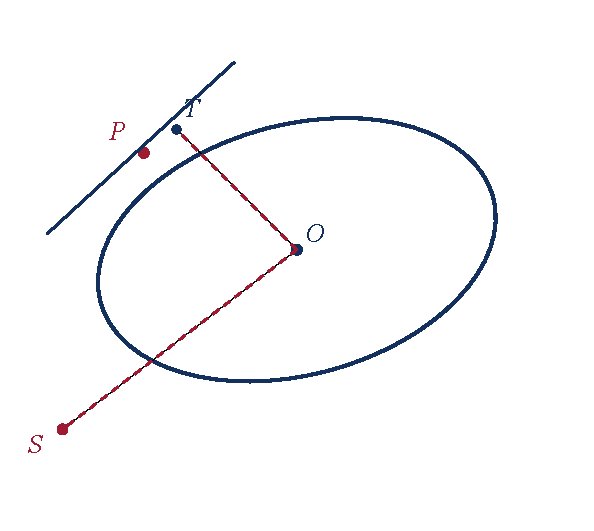
\includegraphics[width=0.5\textwidth]{figuras/pdf/cap06-fig1.pdf}
\caption{El elipsoide $\mathrm F=1$: el punto $\mathrm P$, el plano
tangente en $\mathrm P$, el pie de la perpendicular $\mathrm T$ desde el
centro $\mathrm O$, y el punto $\mathrm S$ sobre $\mathrm{OT}$ tal que
$\mathrm{OS}=1/\mathrm{OT}$.}
\label{fig:cap6-1}
\end{figure}

\section{Superficie de onda. Propagación rectilínea de la luz}

\subsection{Superficie de onda}

\noindent\textbf{180. Superficie de onda.} — Si suponemos el éter
primitivamente en reposo y que, en el origen de los tiempos, se perturban
las moléculas contenidas en una esfera de radio muy pequeño, las moléculas
en movimiento al cabo de la unidad de tiempo pertenecerán a una cierta
superficie que se llama \emph{superficie de onda}.

Esta superficie es una esfera en un medio isótropo. Extendiendo a los
cuerpos no isótropos el principio de Huygens, se puede hallar la ecuación
de la superficie de onda en esos medios cuando se conoce la velocidad de
propagación de una onda plana. Pero se pueden hacer a esta extensión del
principio de Huygens las objeciones que señalamos en el caso de los
isótropos, y para ser rigurosos, nos haría falta reemprender para los
cuerpos anisótropos la justificación a la que llegamos en el capítulo III.
Nos limitaremos a admitir la manera de razonar de Huygens sin buscar su
justificación.

Consideremos una onda plana $PP'$ (figura~\ref{fig:cap6-2}) que pasa por
un punto $O$ de un medio anisótropo. Al cabo de la unidad de tiempo, esta
onda coincidirá con el plano $QQ'$ paralelo a $PP'$, y situado a una
distancia de este último plano igual a la velocidad de propagación $V$ de
esta onda.

Por otra parte, la perturbación inicial del punto $O$ pondrá en
movimiento, al cabo del tiempo $1$, las moléculas del medio elástico que,
según la definición de la superficie de onda, están situadas en la
superficie de onda $S$ relativa al punto $O$. Ahora bien, según el
principio de Huygens, el movimiento del éter en todo punto de la onda
plana $QQ'$ es la resultante de los movimientos que envían aisladamente
cada uno de los puntos $O,O'$ de la onda $PP'$. Siendo $S,S',\dots$ las
ondas elementales de estos puntos, no puede haber movimiento más allá del
plano tangente común $Q_1Q_1'$ a estas ondas.\footnote{Corrección indicada
en la fe de erratas del propio volumen original, que pide rotular $Q_1Q_1'$
la recta superior de la figura, impresa también como $QQ'$.~(N.~del T.)} Además, lo hay ciertamente
en el punto $Q_1$ donde este plano toca a la superficie $S$; pues,
$Q_1$ siendo exterior a las demás superficies de onda $S',\dots$, el
movimiento enviado a $Q_1$ por el punto $O$ no puede ser destruido por el
movimiento enviado por los demás puntos del plano $PP'$. Y como el
movimiento no debe tener lugar más que en el plano $QQ'$, los dos planos
$QQ'$ y $Q_1Q_1'$ deben confundirse.

Cualquiera que sea la dirección del plano de la onda $PP'$ que pasa por el
punto $O$, la superficie de onda de este punto será siempre tangente a la
posición ocupada por la onda plana al cabo de la unidad de tiempo; por
consiguiente, es la envolvente de estas posiciones.

\begin{figure}[ht]
\centering
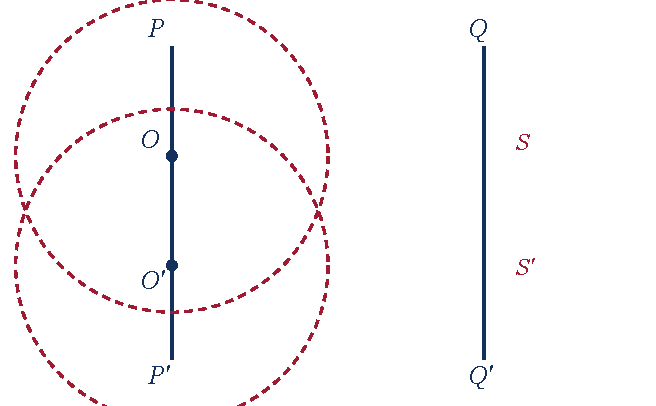
\includegraphics[width=0.75\textwidth]{figuras/pdf/cap06-fig2.pdf}
\caption{Dos posiciones sucesivas de una onda plana, $PP'$ y $QQ'$; las
ondas elementales $S,S'$ de los puntos $O,O'$ y su plano tangente común
$Q_1Q_1'$, que según el principio de Huygens debe confundirse con $QQ'$.}
\label{fig:cap6-2}
\end{figure}

\subsection{Dirección del rayo luminoso}

\noindent\textbf{181. Dirección del rayo luminoso.} — He aquí cómo se
puede, apoyándose en el principio de Huygens, determinar la dirección del
rayo luminoso. Sea $P$ (figura~\ref{fig:cap6-3}) la posición del plano de
la onda en un instante cualquiera, y $P'$ la nueva posición del plano de
la onda al cabo de la unidad de tiempo.

Supongamos ahora que el plano $P$ no esté perturbado en su totalidad, y
que la parte iluminada de este plano se reduzca a un elemento $AB$, con su
centro de gravedad en $O$, muy pequeño en términos absolutos, pero lo
bastante grande, sin embargo, para que puedan despreciarse los fenómenos
de difracción.

Se obtendrá la porción iluminada del plano $P'$ construyendo las
superficies de onda que tienen por centros los diversos puntos de $AB$, y
se buscarán los puntos de contacto de estas superficies con el plano $P'$.
Los puntos así obtenidos formarán un elemento plano $A'B'$ con su centro
de gravedad en $O'$. La recta $OO'$ es entonces el rayo luminoso buscado,
de donde la siguiente regla:

\begin{enunciado}{Regla de Huygens para el rayo luminoso}
Se obtendrá la dirección del rayo luminoso uniendo el punto $O$ al punto
de contacto de la superficie de onda, que tiene su centro en $O$, con un
plano tangente paralelo al plano de la onda.
\end{enunciado}

Vamos a aplicar esta regla sin preocuparnos por las objeciones que suscita
el principio de Huygens. Daremos, por lo demás, más adelante (§189) una
demostración rigurosa.

\begin{figure}[ht]
\centering
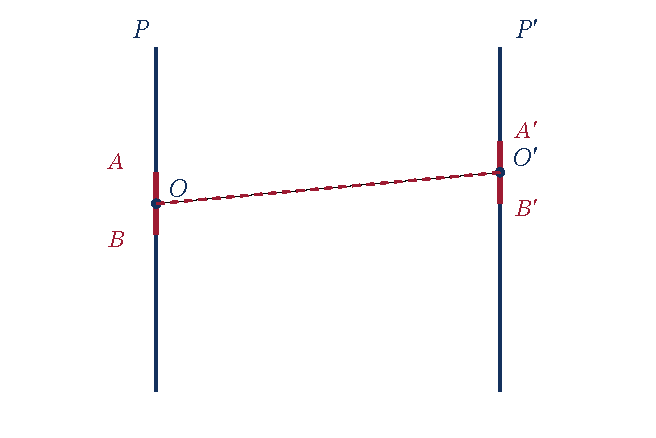
\includegraphics[width=0.6\textwidth]{figuras/pdf/cap06-fig3.pdf}
\caption{Construcción del rayo luminoso: el elemento iluminado $AB$ del
plano $P$, su imagen $A'B'$ en el plano $P'$, y el rayo $OO'$.}
\label{fig:cap6-3}
\end{figure}

\noindent\textbf{182.} Sean $\alpha,\beta,\gamma$ los cosenos directores
de la normal a una onda plana, $V$ la velocidad de propagación de esta
onda, y $x,y,z$ las coordenadas del punto donde la superficie de onda es
encontrada por el rayo luminoso que pasa por el origen. Perteneciendo
este punto al plano ocupado por la onda al cabo de la unidad de tiempo,
sus coordenadas satisfacen la ecuación
\begin{equation}
\alpha x+\beta y+\gamma z=\mathrm V;
\tag{1}
\end{equation}
como pertenece igualmente a la envolvente de este plano, se tiene también
\begin{equation}
x\,d\alpha+y\,d\beta+z\,d\gamma=d\mathrm V.
\tag{2}
\end{equation}
En cuanto a la velocidad de propagación $V$, sabemos que en todas las
teorías de la doble refracción que hemos expuesto, está dada por la
ecuación
\begin{equation}
\frac{\alpha^2}{\mathrm V^2-a}+\frac{\beta^2}{\mathrm V^2-b}+\frac{\gamma^2}{\mathrm V^2-c}=\mathrm F(\alpha,\beta,\gamma,\mathrm V)=0,
\tag{3}
\end{equation}
que, por diferenciación, da
\[
\frac{d\mathrm F}{d\alpha}d\alpha+\frac{d\mathrm F}{d\beta}d\beta+\frac{d\mathrm F}{d\gamma}d\gamma+\frac{d\mathrm F}{d\mathrm V}d\mathrm V=0.
\]
Reemplazando aquí $d\mathrm V$ por el primer miembro de la igualdad (2),
esta ecuación se convierte en
\begin{equation}
\Bigl(\frac{d\mathrm F}{d\alpha}+x\frac{d\mathrm F}{d\mathrm V}\Bigr)d\alpha
+\Bigl(\frac{d\mathrm F}{d\beta}+y\frac{d\mathrm F}{d\mathrm V}\Bigr)d\beta
+\Bigl(\frac{d\mathrm F}{d\gamma}+z\frac{d\mathrm F}{d\mathrm V}\Bigr)d\gamma=0.
\tag{4}
\end{equation}
Por lo demás, $\alpha,\beta,\gamma$ están ligados por la relación
$\alpha^2+\beta^2+\gamma^2=1$, que da por diferenciación
\begin{equation}
\alpha\,d\alpha+\beta\,d\beta+\gamma\,d\gamma=0.
\tag{5}
\end{equation}
Las dos relaciones (4) y (5), satisfechas a la vez para todos los valores
que se puedan dar a $d\alpha$ y $d\beta$, deben ser idénticas; tendremos,
pues, introduciendo una constante arbitraria $\mathrm K$,
\begin{equation}
\frac{d\mathrm F}{d\alpha}+x\frac{d\mathrm F}{d\mathrm V}=\mathrm K\alpha,\qquad
\frac{d\mathrm F}{d\beta}+y\frac{d\mathrm F}{d\mathrm V}=\mathrm K\beta,\qquad
\frac{d\mathrm F}{d\gamma}+z\frac{d\mathrm F}{d\mathrm V}=\mathrm K\gamma.
\tag{6}
\end{equation}

Busquemos los valores de $K$ y de las
derivadas parciales que entran en estas ecuaciones. Para ello recordemos
que la velocidad de propagación $V$ satisface las ecuaciones
\begin{equation}
\mathrm{AV}^2=a\mathrm A-\alpha\mathrm H,\qquad
\mathrm{BV}^2=b\mathrm B-\beta\mathrm H,\qquad
\mathrm{CV}^2=c\mathrm C-\gamma\mathrm H,
\tag{I}
\end{equation}
donde
\[
\mathrm H=\mathrm Aa\alpha+\mathrm Bb\beta+\mathrm Cc\gamma,
\]
y que, por eliminación de $H$, nos condujeron (§154) a la ecuación (3).
Tendremos
\[
\frac{d\mathrm F}{d\alpha}=\frac{2\alpha}{\mathrm V^2-a},
\]
y, reemplazando $\mathrm V^2-a$ por su valor tomado de la primera de las
ecuaciones del grupo (I),
\[
\frac{d\mathrm F}{d\alpha}=-\frac{2\mathrm A}{\mathrm H}.
\]
Hallaremos, de la misma manera, $d\mathrm F/d\beta=-2\mathrm B/\mathrm H$,
$d\mathrm F/d\gamma=-2\mathrm C/\mathrm H$.

Para la derivada respecto de $V$ tendremos
\[
\frac{d\mathrm F}{d\mathrm V}=-\sum\frac{2\alpha^2\mathrm V}{(\mathrm V^2-a)^2}
=-2\mathrm V\sum\frac{\alpha^2}{(\mathrm V^2-a)^2}
=-\frac{2\mathrm V}{\mathrm H^2}\sum\mathrm A^2.
\]
Ahora bien, hemos visto (§155) que si el punto $A,B,C$ está sobre el
elipsoide de elasticidad, se tiene
\[
\mathrm V=\frac{1}{\sqrt{\mathrm A^2+\mathrm B^2+\mathrm C^2}};
\]
resulta
\[
\frac{d\mathrm F}{d\mathrm V}=-\frac{2\mathrm V}{\mathrm H^2}\cdot\frac{1}{\mathrm V^2}=-\frac{2}{\mathrm{VH}^2}.
\]

Calculemos el coeficiente $K$. Para ello multipliquemos las ecuaciones (6)
por $\alpha,\beta,\gamma$ y sumemos; tendremos
\[
\mathrm K=\sum\alpha\frac{d\mathrm F}{d\alpha}+\frac{d\mathrm F}{d\mathrm V}\sum\alpha x;
\]
pero
\[
\sum\alpha\frac{d\mathrm F}{d\alpha}=-\sum\frac{2\mathrm A\alpha}{\mathrm H}=0,
\]
y, según la ecuación (1), $\sum\alpha x=\mathrm V$. Por consiguiente
\[
\mathrm K=\frac{d\mathrm F}{d\mathrm V}\,\mathrm V=-\frac{2}{\mathrm H^2}.
\]
Llevando estos valores de $K$ y de las derivadas parciales a las
ecuaciones (6), y multiplicando después por $-\mathrm H^2/2$,\footnote{El
original dice «multipliant par $-\frac{2}{\mathrm H^2}$»; es por
$-\frac{\mathrm H^2}{2}$ por lo que hay que multiplicar para obtener las
ecuaciones (II).~(N.~del T.)}
obtendremos
\begin{equation}
\mathrm{AH}+\frac{x}{\mathrm V}=\alpha,\qquad
\mathrm{BH}+\frac{y}{\mathrm V}=\beta,\qquad
\mathrm{CH}+\frac{z}{\mathrm V}=\gamma,
\tag{II}
\end{equation}
ecuaciones que nos darán las coordenadas $x,y,z$ del punto de
intersección de la superficie de onda por el rayo luminoso.

\subsection{Relaciones entre la dirección del rayo luminoso y las de las
vibraciones}

\noindent\textbf{183. Relaciones entre la dirección del rayo luminoso y
las de las vibraciones.} — Consideremos la vibración de Neumann, cuyos cosenos directores son
proporcionales a $A',B',C'$. Si multiplicamos las ecuaciones del grupo
(II) por $A',B',C'$ obtenemos, para la suma de estos productos,
\[
\mathrm H\sum\mathrm{AA}'+\frac1{\mathrm V}\sum\mathrm A'x=\sum\mathrm A'\alpha.
\]
Sabemos, por lo demás, que la vibración de Neumann está situada en el
plano de la onda y que es perpendicular a la de Fresnel; por consiguiente,
tendremos
\[
\mathrm A'\alpha+\mathrm B'\beta+\mathrm C'\gamma=0,\qquad
\mathrm{AA}'+\mathrm{BB}'+\mathrm{CC}'=0,
\]
y la relación precedente se reducirá a la siguiente
\[
\mathrm A'x+\mathrm B'y+\mathrm C'z=0,
\]
que expresa que \emph{la vibración de Neumann es perpendicular al rayo
luminoso}.

Tomemos ahora la vibración de M.~Sarrau, cuyos cosenos directores son
proporcionales a $\mathrm{A}a,\mathrm{B}b,\mathrm{C}c$. Multiplicando
respectivamente cada una de las ecuaciones (II) por estas cantidades y
sumando, tenemos
\[
\mathrm H\sum a\mathrm A^2+\frac1{\mathrm V}\sum a\mathrm Ax=\sum\mathrm Aa\alpha.
\]
El punto de coordenadas $A,B,C$ estando sobre el elipsoide de elasticidad,
$\sum a\mathrm A^2=1$; por otra parte, por hipótesis, $\mathrm
H=\sum\mathrm Aa\alpha$. Por consiguiente, la relación precedente se
reduce a la siguiente
\[
a\mathrm Ax+b\mathrm By+c\mathrm Cz=0,
\]
que expresa que \emph{la vibración de M.~Sarrau es perpendicular al rayo
luminoso}.

\subsection{Ecuación de la superficie de onda}

\noindent\textbf{184. Ecuación de la superficie de onda.} — La ecuación
de esta superficie se obtendrá eliminando $\alpha,\beta,\gamma,A,B,C$ y
$V$ entre las ecuaciones que forman los grupos (I) y (II) y la siguiente
\begin{equation}
\mathrm{A}ax+\mathrm{B}by+\mathrm{C}cz=0,
\tag{IV}
\end{equation}
que acabamos de deducir del grupo (II).

La primera de las ecuaciones (II) puede escribirse
\[
\frac{x\mathrm H}{\mathrm V}=\alpha\mathrm H-\mathrm{AH}^2,
\]
y la primera de las ecuaciones (I) nos da
\[
\alpha\mathrm H=\mathrm A(a-\mathrm V^2).
\]
Tendremos, pues,
\[
\frac{x\mathrm H}{\mathrm V}=\mathrm A(a-\mathrm V^2-\mathrm H^2).
\]
Busquemos el valor de $V^2+H^2$. Para ello saquemos de las ecuaciones
(II) los valores de $x,y,z$ y formemos los cuadrados de estas cantidades;
tendremos:
\[
x=\alpha\mathrm V-\mathrm{AHV},\qquad x^2=\alpha^2\mathrm V^2-2\mathrm A\alpha\mathrm{HV}^2+\mathrm A^2\mathrm H^2\mathrm V^2,
\]
\[
y=\beta\mathrm V-\mathrm{BHV},\qquad y^2=\beta^2\mathrm V^2-2\mathrm B\beta\mathrm{HV}^2+\mathrm B^2\mathrm H^2\mathrm V^2,
\]
\[
z=\gamma\mathrm V-\mathrm{CHV},\qquad z^2=\gamma^2\mathrm V^2-2\mathrm C\gamma\mathrm{HV}^2+\mathrm C^2\mathrm H^2\mathrm V^2,
\]
y por consiguiente
\[
x^2+y^2+z^2=r^2=\mathrm V^2-2\mathrm{HV}^2\sum\mathrm A\alpha+\mathrm H^2\mathrm V^2\sum\mathrm A^2.
\]
Ya hemos visto que $\sum\mathrm A\alpha=0$ y $\sum\mathrm A^2=1/\mathrm
V^2$; por consiguiente tendremos, para el cuadrado del radio vector de la
superficie de onda,
\[
r^2=\mathrm V^2+\mathrm H^2.
\]
Llevando este valor de $V^2+H^2$ a la expresión antes obtenida de
$xH/V$, obtendremos
\[
\frac{x\mathrm H}{\mathrm V}=\mathrm A(a-r^2),\qquad\text{o bien}\qquad
\frac{x}{r^2-a}=-\frac{\mathrm{AV}}{\mathrm H},
\]
y, por simetría,
\[
\frac{y}{r^2-b}=-\frac{\mathrm{BV}}{\mathrm H},\qquad
\frac{z}{r^2-c}=-\frac{\mathrm{CV}}{\mathrm H}.
\]
Tenemos así cantidades proporcionales a $A,B,C$ que, llevadas en lugar de
$A,B,C$ a la ecuación (IV), nos darán
\[
\frac{ax^2}{r^2-a}+\frac{by^2}{r^2-b}+\frac{cz^2}{r^2-c}=0;
\]
esta es la ecuación de la superficie de onda bajo su forma más simple.

Esta superficie parece ser de sexto grado; es fácil mostrar, desarrollando
la ecuación precedente, que es solamente de cuarto grado. Se tendrá,
quitando los denominadores,\footnote{El original imprime
$\sum ax^2(r^2-b^2)(r^2-c^2)=0$; los denominadores son $r^2-b$ y $r^2-c$,
como lo confirma el desarrollo que sigue.~(N.~del T.)}
\[
\sum ax^2(r^2-b)(r^2-c)=0,
\]
o bien
\[
r^4\sum ax^2-r^2\sum(b+c)ax^2+abc(x^2+y^2+z^2)=0.
\]
$r^2$ se encuentra, pues, en factor; suprimiendo este factor se obtiene
\[
\sum x^2\sum ax^2-\sum(ab+ac)x^2+abc=0,
\]
ecuación que no es más que de cuarto grado.

\subsection{Construcción geométrica de la superficie de onda}

\noindent\textbf{185. Construcción geométrica de la superficie de onda.}
— Consideremos una onda plana y tomemos como plano de la figura un plano
perpendicular al plano de onda y que pase por la vibración de Fresnel.
Esta vibración estará representada por la recta $OF$ (figura~\ref{fig:cap6-4}).
La vibración de Neumann, situada en el plano de la onda y perpendicular a
la de Fresnel, será normal al plano de la figura y se proyectará en el
punto $O$. El rayo luminoso y la vibración de M.~Sarrau, ambos
perpendiculares a la vibración de Neumann, estarán situados en el plano
del cuadro; sean $OS$ la vibración de M.~Sarrau, $OM$ el rayo luminoso,
rectas que son rectangulares entre sí. La posición del plano de la onda
al cabo de la unidad de tiempo está representada por su traza $PM$.

El plano tangente al elipsoide de elasticidad $ax^2+by^2+cz^2=1$ en el
punto $F$ de coordenadas $A,B,C$ tiene por ecuación
\[
a\mathrm Ax+b\mathrm By+c\mathrm Cz=1.
\]
Los cosenos directores de la normal a este plano son proporcionales a
$a\mathrm A,b\mathrm B,c\mathrm C$, es decir, a las componentes de la
vibración de M.~Sarrau. Este plano tangente será, pues, perpendicular al
plano de la figura, en la cual estará representado por la perpendicular
$FQ$ sobre $OS$. — Este resultado puede obtenerse de otra manera. La
recta $OF$ es un eje de la elipse de intersección $E$ del elipsoide de
elasticidad por el plano de la onda; por consiguiente, la tangente en $F$
a esta elipse es perpendicular a $OF$, y, estando además situada en el
plano de la onda, perpendicular al plano de la figura, es ella misma
perpendicular a este último plano. El plano tangente al elipsoide en $F$
que contiene esta tangente será también perpendicular al plano de la
figura.

Consideremos la esfera descrita desde el punto $O$ como centro con un
radio igual a la unidad. Si tomamos sobre la recta $OQ$ una longitud
$OS=1/OQ$, el punto $S$ es el polo del plano $FQ$ respecto a esta esfera.
Por consiguiente, el lugar del punto $S$ cuando el punto $F$ describe el
elipsoide de elasticidad será la polar recíproca del elipsoide de
elasticidad. Este elipsoide recíproco tiene, pues, por ecuación
\[
\frac{x^2}{a}+\frac{y^2}{b}+\frac{z^2}{c}=1.
\]
Tracemos el plano tangente en $S$ a este elipsoide; tiene por polo el
punto $F$; por consiguiente, es perpendicular al rayo $OF$, y corta el
plano de la figura según $ST$. Vamos a deducir que la recta $OS$ es un
eje de la elipse de intersección $E'$ del elipsoide recíproco $S$ por un
plano perpendicular al rayo luminoso. En efecto, la tangente en $S$ a esta
elipse está situada en el plano de sección y en el plano tangente al
elipsoide; estando estos dos planos perpendiculares al plano de la
figura, la tangente es también perpendicular a este último plano, y, por
consiguiente, al radio vector $OS$, que debe entonces ser un eje.

Mostremos ahora que se tiene $OM=OS$. Las rectas $OM$ y $OP$ siendo
respectivamente perpendiculares a $OS$ y $OF$, los ángulos $FOS$ y $POM$
son iguales. Tendremos, pues, puesto que $OP$, velocidad de propagación
normal de una onda plana, es igual al inverso del eje $OF$ de la elipse
$E$,
\[
OM=\frac{OP}{\cos\theta}=\frac{1}{OF\cos\theta}.
\]
Por otra parte, el triángulo $OFQ$ nos da
\[
OS=\frac{1}{OQ}=\frac{1}{OF\cos\theta}.
\]
Tenemos, pues, en efecto, $OM=OS$.

El punto $M$ siendo un punto de la superficie de onda, podremos construir
esta superficie de la manera siguiente: cortar el elipsoide recíproco $S$
por un plano cualquiera, y llevar sobre la normal $OM$ a este plano
longitudes iguales a los ejes de la elipse $E'$ de intersección.

\begin{figure}[ht]
\centering
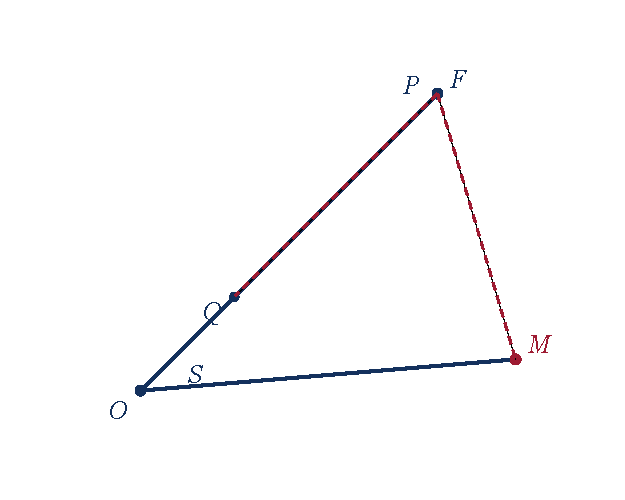
\includegraphics[width=0.85\textwidth]{figuras/pdf/cap06-fig4.pdf}
\caption{Construcción geométrica de la superficie de onda: la vibración
de Fresnel $OF$, el punto $Q$, la vibración de M.~Sarrau $OS$ y el rayo
luminoso $OM$.}
\label{fig:cap6-4}
\end{figure}

\subsection{Secciones de la superficie de onda por los planos de simetría}

\noindent\textbf{186. Secciones de la superficie de onda por los planos
de simetría.} — Tomemos como planos de la figura uno de los tres planos
de simetría óptica del medio. Siendo estos planos los planos principales
del elipsoide de elasticidad, serán igualmente los planos principales del
elipsoide recíproco $S$. Un plano perpendicular al plano de la figura y
que pase por el centro de este elipsoide contendrá, pues, uno de sus
ejes, el que es perpendicular al plano de la figura. Si $OS$
(figura~\ref{fig:cap6-5}) es el plano de sección considerado, se tendrán
los dos puntos correspondientes de la superficie de onda llevando sobre
la normal $OM$ a este plano la longitud $OM=OS$ y la longitud $OM'$ igual
al eje proyectado en $O$. Los dos puntos $M$ y $M'$ están situados en el
plano de la figura, y se obtendrá la intersección de la superficie de
onda por este plano haciendo girar el plano $OS$ alrededor de la normal
que pasa por $O$. Siendo constante uno de los ejes de las secciones así
obtenidas, el eje proyectado en $O$, la longitud $OM'$ será constante y
el punto $M'$ describirá un círculo. El punto $M$ describirá una elipse
que no es otra que la elipse $AB$ de intersección del elipsoide
recíproco por el plano de la figura, elipse cuyos ejes se han hecho girar
$90^{\circ}$.

La intersección de la superficie de onda por cada uno de los planos de
simetría se compone, pues, de un círculo y de una elipse. El conocimiento
de estas intersecciones permite darse bastante bien cuenta de la forma de
la superficie de onda. Si suponemos que se tenga $a>b>c$, la parte de la
superficie de onda comprendida en el triedro donde las tres coordenadas de
un punto son positivas tendrá la forma representada por la
figura~\ref{fig:cap6-6}.

En el caso particular de cristales de un eje, el elipsoide de elasticidad
es de revolución; el elipsoide recíproco, y por consiguiente la superficie
de onda, lo son igualmente. La intersección de esta superficie por dos de
los planos de simetría se compone de una elipse y de un círculo; la
intersección por el tercer plano de simetría está formada por dos
círculos. — La superficie de onda se compone entonces de una esfera y de
un elipsoide de revolución tangentes.

\begin{figure}[ht]
\centering
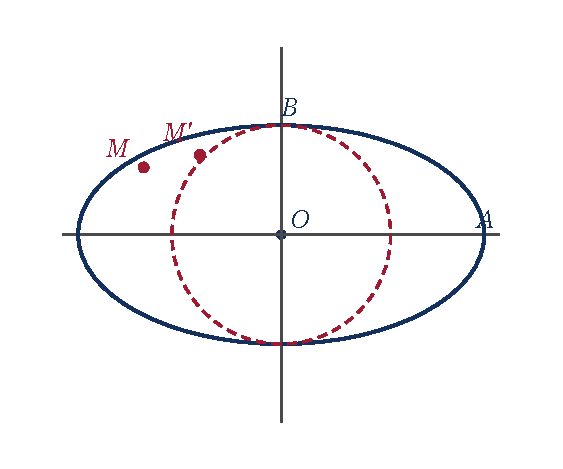
\includegraphics[width=0.75\textwidth]{figuras/pdf/cap06-fig5.pdf}
\caption{Sección de la superficie de onda por un plano de simetría: el
círculo y la elipse $AB$ del elipsoide recíproco.}
\label{fig:cap6-5}
\end{figure}

\begin{figure}[ht]
\centering
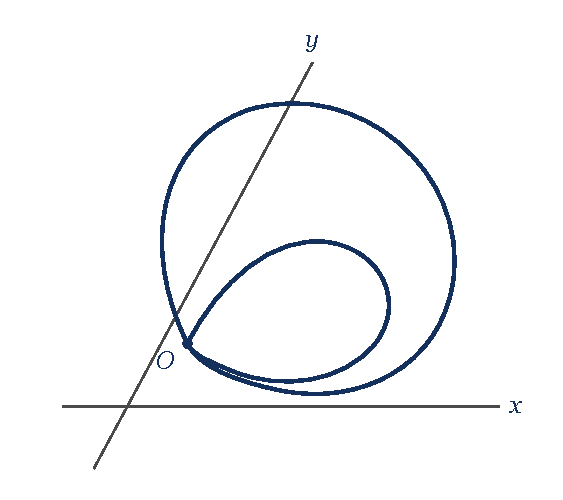
\includegraphics[width=0.6\textwidth]{figuras/pdf/cap06-fig6.pdf}
\caption{Forma de la superficie de onda en el triedro de coordenadas
positivas, para $a>b>c$: la curva compuesta que resulta de las dos hojas
(elipsoidal y esférica) de la superficie.}
\label{fig:cap6-6}
\end{figure}

\subsection{Ombligos y planos tangentes singulares de la superficie de
onda}

\noindent\textbf{187. Ombligos y planos tangentes singulares de la
superficie de onda.} — Consideremos un plano cíclico del elipsoide
recíproco. Todos los radios vectores de esta sección serán ejes iguales; por
consiguiente, a un plano cíclico no corresponde más que un solo punto $M$
de la superficie de onda. Pero, a cada dirección $OS$ de un eje
corresponde un plano tangente normal al plano que pasa por $OS$ y $OM$;
tendremos, pues, una infinidad de planos tangentes en $M$. Es un punto
cónico. Como a cada sección cíclica corresponden dos puntos cónicos,
tendremos cuatro puntos cónicos reales y ocho puntos cónicos imaginarios.
A estos puntos se les llama también los \emph{ombligos} de la superficie
de onda.

El cono formado por los planos tangentes a la superficie de onda en un
punto cónico es de segundo grado. En efecto, no puede ser de tercer
grado, pues la recta que pasa por dos de estos puntos encontraría a la
superficie en seis puntos, lo que no puede ocurrir puesto que esta
superficie es de cuarto grado.

La consideración de los planos cíclicos del elipsoide de elasticidad
conduce a una nueva propiedad interesante de la superficie de onda.

Si suponemos que el plano de la onda sea un plano cíclico, todo radio del
círculo de intersección será una dirección de la vibración de Fresnel. A
cada una de estas direcciones corresponde un plano tangente $PM$ a la
superficie de onda; pero, como $OP=1/OF$ y $OF$ es constante, estos
diversos planos tangentes se confunden. Sus puntos de contacto con la
superficie de onda no se confunden, sin embargo, pues a cada dirección de
$OF$ corresponde una dirección particular de $OS$ y, por consiguiente, de
$OM$. Por consiguiente, el plano $PM$ correspondiente a una sección
circular del elipsoide toca la superficie de onda en una infinidad de
puntos distintos. Estos puntos forman una curva que debe ser de segundo
grado, pues, en general, la sección de una superficie por un plano
tangente singular, componiéndose de dos curvas confundidas, cada una de
estas curvas es de un grado igual a la mitad del grado de la superficie.
Además, esta curva de segundo grado es un círculo. En efecto, las
direcciones asintóticas de la superficie están dadas por los términos del
más alto grado $\sum x^2\sum ax^2$; dos de estas direcciones son las de
un círculo, y, como para los planos tangentes singulares las direcciones
asintóticas deben confundirse dos a dos, puesto que las curvas de
intersección se confunden, las cuatro direcciones asintóticas son las de
círculos. La curva de intersección de la superficie por un plano tangente
singular se compone, pues, de dos círculos confundidos. Habrá cuatro de
estos planos tangentes singulares, que serán reales, un elipsoide teniendo
dos direcciones de secciones cíclicas a cada una de las cuales
corresponden dos planos tangentes singulares.

Muchas otras propiedades de la superficie de onda han sido estudiadas por
diversos matemáticos. En particular, citaremos los procedimientos
elegantes indicados por M.~Mannheim para hallar los radios de curvatura y
trazar las líneas de curvatura de la superficie de onda. Pero no
insistiremos en estas propiedades, que no tienen ningún interés desde el
punto de vista de la óptica. Solo la consideración de los ombligos y de
los planos tangentes singulares tiene una gran importancia. Se sabe, en
efecto, que condujo a Hamilton al descubrimiento de la \emph{refracción
cónica interior} y de la \emph{refracción cónica exterior} que Lloyd pudo
poner en evidencia mediante experiencias delicadas.

\begin{notahistorica}
La refracción cónica, predicha teóricamente por William Rowan Hamilton en
1832 a partir de los puntos cónicos y de los planos tangentes singulares
de la superficie de onda de Fresnel, fue confirmada experimentalmente muy
poco después por Humphrey Lloyd, quien la observó en el aragonito y
publicó sus resultados en 1833. Es uno
de los ejemplos más citados de un fenómeno físico descubierto primero por
el análisis matemático y solo después observado en el laboratorio.
\end{notahistorica}

\section{Propagación rectilínea de la luz}

\subsection{Propagación rectilínea de la luz en un medio isótropo}

\noindent\textbf{188. Propagación rectilínea de la luz en un medio
isótropo.} — Hemos determinado más arriba (§181) la dirección del rayo
luminoso en un medio cristalizado apoyándonos en el principio de Huygens;
pero este principio, cualesquiera que sean la utilidad y la importancia de
su papel en óptica, se presta a un gran número de objeciones de las que
hemos tratado de dar una idea en la primera parte del curso.

Por eso no será inútil explicar aquí cómo se puede determinar la
dirección del rayo luminoso en un medio isótropo o anisótropo
independizándose del principio de Huygens y de las dificultades sin
cuento que suscita. Comenzaremos por el caso más simple, que es el de los
medios isótropos, y escribiremos las ecuaciones del movimiento
transversal bajo la forma habitual,
\[
\rho\,\frac{d^2\xi}{dt^2}=\Delta\xi,\qquad
\rho\,\frac{d^2\eta}{dt^2}=\Delta\eta,\qquad
\rho\,\frac{d^2\zeta}{dt^2}=\Delta\zeta,
\]
con $\Theta=0$.

Busquemos satisfacer estas ecuaciones haciendo:
\begin{equation}
\xi=Ae^{\mathrm P},\qquad \eta=Be^{\mathrm P},\qquad \zeta=Ce^{\mathrm P},
\tag{1}
\end{equation}
donde
\[
\mathrm P=\frac{2i\pi}{\lambda}(z-\mathrm Vt).
\]
Si consideráramos $A,B,C$ como constantes, caeríamos de nuevo en la
teoría ordinaria de la propagación de una onda plana indefinida. Pero
entonces la cuestión de la dirección del rayo luminoso no se plantearía,
puesto que todo el espacio quedaría igualmente iluminado. Debemos, pues,
suponer que solo una porción del éter es agitada por ondulaciones y, por
consiguiente, que $A,B,C$ son funciones de $x,y,z$ y $t$.

Tomaremos una unidad de longitud comparable a nuestras unidades
habituales, de tal manera que $\lambda$ será una longitud muy pequeña y
$2i\pi/\lambda$ una cantidad infinitamente grande; (si en la exposición
de la teoría de M.~Sarrau consideramos esta cantidad como muy pequeña, es
porque habíamos tomado una unidad de longitud comparable a la distancia
que separa dos moléculas materiales). Por el contrario, supondremos que
las funciones $A,B,C$ y sus derivadas de los diversos órdenes son
finitas.

Las consideraciones que siguen no se aplican, pues, al menos sin
modificación, al caso en que las funciones $A,B,C$ son discontinuas y en
que, por consiguiente, sus derivadas no son finitas; en ese caso, en
efecto, se producen fenómenos de difracción y hay desviación del rayo
luminoso.

Sustituyamos los valores (1) en la primera de las ecuaciones del
movimiento; vendrá, dividiendo por $-e^{\mathrm P}4\pi^2/\lambda^2$,
\[
\rho\Bigl(\mathrm V^2\mathrm A-\frac{\lambda}{i\pi}\mathrm V\frac{dA}{dt}-\frac{\lambda^2}{4\pi^2}\frac{d^2A}{dt^2}\Bigr)
=A+\frac{\lambda}{i\pi}\frac{dA}{dz}-\frac{\lambda^2}{4\pi^2}\Delta A.
\]
Despreciaremos los términos en $\lambda^2$; si observamos que $\rho
V^2=1$, veremos que los términos independientes de $\lambda$
desaparecen; los dos miembros contendrán entonces el factor $\lambda/i\pi$.
Si hacemos desaparecer este factor, quedará simplemente
\begin{equation}
\frac{dA}{dt}+\mathrm V\frac{dA}{dz}=0.
\tag{2}
\end{equation}
Se hallaría del mismo modo
\[
\frac{dB}{dt}+\mathrm V\frac{dB}{dz}=0,\qquad
\frac{dC}{dt}+\mathrm V\frac{dC}{dz}=0.
\]
Si sustituimos los valores (1) en la ecuación $\Theta=0$ y la dividimos
por $e^{\mathrm P}$, vendrá
\[
\frac{2i\pi}{\lambda}C+\frac{dA}{dx}+\frac{dB}{dy}+\frac{dC}{dz}=0.
\]
Esta ecuación nos muestra que $C$ es un infinitamente pequeño del mismo
orden que $\lambda$. En cuanto a la ecuación (2), tiene por integral
general:
\[
A=\text{función arbitraria de }x,y\text{ y }z-\mathrm Vt.
\]
Así, el valor de $A$ en el tiempo $t$ y en el punto cuyas coordenadas son
$x,y$ y $z+\mathrm Vt$, será el mismo que en el tiempo $0$ y en el punto
$x,y,z$. Si en el origen de los tiempos no hay luz sensible más que en el
interior de una pequeña esfera que tenga por centro el punto $x,y,z$; en
la época $t$, no habrá luz sensible más que en el interior de una
pequeña esfera del mismo radio que tenga por centro el punto $x,y$ y
$z+\mathrm Vt$. En otros términos, la luz se habrá propagado en la
dirección del eje de las $z$, es decir, perpendicularmente al plano de la
onda.

Así, \emph{en un medio isótropo el rayo luminoso es normal al plano de la
onda.}

\subsection{Propagación rectilínea de la luz en un medio anisótropo}

\noindent\textbf{189. Propagación rectilínea de la luz en un medio
anisótropo.} — Pasemos al caso de un medio cristalizado, y tomemos por
ejemplo las ecuaciones de M.~Sarrau:
\begin{equation}
\frac1a\frac{d^2\xi}{dt^2}=\Delta\xi-\frac{d\Theta}{dx},\qquad
\frac1b\frac{d^2\eta}{dt^2}=\Delta\eta-\frac{d\Theta}{dy},\qquad
\frac1c\frac{d^2\zeta}{dt^2}=\Delta\zeta-\frac{d\Theta}{dz}.
\tag{1}
\end{equation}
Busquemos satisfacerlas poniendo
\[
\xi=\mathrm Le^{\mathrm P},\qquad \eta=\mathrm Me^{\mathrm P},\qquad
\zeta=\mathrm Ne^{\mathrm P},\qquad
\mathrm P=\frac{2i\pi}{\lambda}(\alpha x+\beta y+\gamma z-\mathrm Vt),
\]
siendo $L,M,N$ funciones de $x,y,z$ y $t$.

Si $L,M$ y $N$ debieran ser constantes $L_0,M_0,N_0$, estas constantes y
$V$ deberían satisfacer las ecuaciones\footnote{El original numera
también (1) este sistema, repitiendo el número de las ecuaciones del
movimiento que preceden; conservamos su numeración.~(N.~del T.)}
\begin{equation}
\frac{\mathrm V^2\mathrm L_0}{a}=\mathrm L_0-\alpha\mathrm H,\qquad
\frac{\mathrm V^2\mathrm M_0}{b}=\mathrm M_0-\beta\mathrm H,\qquad
\frac{\mathrm V^2\mathrm N_0}{c}=\mathrm N_0-\gamma\mathrm H,
\tag{1}
\end{equation}
\[
\mathrm H=\alpha\mathrm L_0+\beta\mathrm M_0+\gamma\mathrm N_0.
\]
Pongamos entonces:
\[
\mathrm L=\mathrm L_0f+g,\qquad \mathrm M=\mathrm M_0f+h,\qquad \mathrm N=\mathrm N_0f,
\]
y busquemos determinar las tres funciones $f,g$ y $h$.

Para obtener estas tres funciones, sustituyamos en las ecuaciones del
movimiento, en lugar de $\xi,\eta,\zeta$, sus valores, es decir,
\[
\xi=(\mathrm L_0f+g)e^{\mathrm P},\qquad \eta=(\mathrm M_0f+h)e^{\mathrm P},\qquad \zeta=\mathrm N_0fe^{\mathrm P}.
\]
Obtendremos así tres ecuaciones diferenciales entre $f,g$ y $h$. Según su
modo de formación, estas ecuaciones serán:

1.\textsuperscript{o} Lineales y homogéneas respecto a $f,g$ y $h$ y a sus
derivadas parciales de los dos primeros órdenes;

2.\textsuperscript{o} De coeficientes constantes, una vez suprimido el
factor común $e^{\mathrm P}$.

Eliminemos ahora $g$ y $h$ entre estas tres ecuaciones; quedará una
ecuación diferencial única que definirá a $f$. Esta ecuación será también
lineal, homogénea y de coeficientes constantes; pero será de orden
superior al segundo.

No contendrá a $f$, pues las ecuaciones del movimiento deben satisfacerse
cuando se hace
\[
f=1,\qquad g=h=0.
\]
No cambiará cuando se multipliquen a la vez $\lambda,x,y,z$ y $t$ por un
mismo factor, lo que equivale a cambiar simultáneamente y en una misma
razón la unidad de longitud y la del tiempo.

Sea
\[
\mathrm A\lambda^p\mathrm D^mf
\]
un término cualquiera del primer miembro de nuestra ecuación; $A$ es una
constante independiente de $\lambda$, y $D^mf$ una de las derivadas
parciales de orden $m$ de $f$. Cuando se cambien $\lambda,x,y,z$ y $t$ en
$k\lambda,kx,ky,kz$ y $kt$, este término quedará multiplicado por
$k^{p-m}$. Para que la ecuación no cambie, es preciso que $m-p$ tenga el
mismo valor para todos los términos de la ecuación. Multiplicaremos
nuestra ecuación por una potencia de $\lambda$ tal que $m-p$ sea igual a
$1$.

Entonces, los coeficientes de las derivadas de primer orden no
contendrán a $\lambda$; los de las derivadas de segundo orden contendrán
el factor $\lambda$; los de las derivadas de tercer orden contendrán el
factor $\lambda^2$; y así sucesivamente. Pero, siendo $\lambda$ muy
pequeño, podemos despreciar los términos que contienen este factor; no
nos quedarán entonces más que las derivadas de primer orden, y la
ecuación en $f$ se escribirá
\[
\mu\frac{df}{dx}+\mu'\frac{df}{dy}+\mu''\frac{df}{dz}+\frac{df}{dt}=0,
\]
siendo $\mu,\mu',\mu''$ constantes.

La integral general de esta ecuación será:
\[
f=\text{función arbitraria de }x-\mu t,\ y-\mu't\text{ y }z-\mu''t,
\]
lo que quiere decir que los cosenos directores del rayo luminoso son
proporcionales a $\mu,\mu'$ y $\mu''$, y que la velocidad de propagación,
estimada no normalmente al plano de la onda, sino en la dirección del
rayo, es $\sqrt{\mu^2+\mu'^2+\mu''^2}$.

Se podrían determinar $\mu,\mu'$ y $\mu''$ efectuando todos los cálculos
que acabamos de indicar; pero esto es inútil. En efecto, las ecuaciones
del movimiento deberán quedar satisfechas si se hace $f=e^{x-\mu t}$, de
donde $g$ y $h$ constante muy pequeña $\times\,e^{x-\mu t}$, y
\[
\mathrm L=\mathrm L_0e^{x-\mu t},\qquad \mathrm M=\mathrm M_0'e^{x-\mu t},\qquad \mathrm N=\mathrm N_0'e^{x-\mu t};
\]
$L_0,M_0'$ y $N_0'$ siendo constantes muy poco diferentes de $L_0,M_0$ y
$N_0$. Tendremos entonces
\[
\xi=\mathrm L_0e^{\mathrm P'},\qquad \eta=\mathrm M_0'e^{\mathrm P'},\qquad \zeta=\mathrm N_0'e^{\mathrm P'};
\]
\[
\mathrm P'=\frac{2i\pi}{\lambda}\Bigl[\Bigl(\alpha+\frac{\lambda}{2i\pi}\Bigr)x+\beta y+\gamma z-\Bigl(\mathrm V+\frac{\lambda\mu}{2i\pi}\Bigr)t\Bigr].
\]
Ahora bien, hemos visto que si $\xi,\eta,\zeta$ son iguales a constantes
multiplicadas por $e^{\mathrm P}$ y que se pone
\[
\mathrm P=\frac{2i\pi}{\lambda}(\alpha x+\beta y+\gamma z-\mathrm Vt)
\]
con $\lambda$ elegido de tal manera que $\alpha^2+\beta^2+\gamma^2=1$,
deberá tenerse
\[
\frac{\alpha^2}{\mathrm V^2-a}+\frac{\beta^2}{\mathrm V^2-b}+\frac{\gamma^2}{\mathrm V^2-c}=0.
\]
Designaremos, como ya lo hemos hecho más arriba, el primer miembro de
esta ecuación por
\[
\mathrm F(\alpha,\beta,\gamma,\mathrm V).
\]
Como $\alpha^2+\beta^2+\gamma^2=1$, tendremos también
\begin{equation}
\mathrm F\Bigl(\alpha,\beta,\gamma,\frac{\mathrm V}{\sqrt{\alpha^2+\beta^2+\gamma^2}}\Bigr)=0.
\tag{3}
\end{equation}
La relación (3), siendo homogénea en $\alpha,\beta,\gamma$ y $V$,
subsistirá aún cuando se hayan multiplicado a la vez $\alpha,\beta,\gamma$
y $V$ por un mismo factor. Es, pues, aún verdadera, incluso cuando ya no
se suponga que la suma $\alpha^2+\beta^2+\gamma^2$ sea igual a $1$.

Así, la relación (3) deberá quedar satisfecha cuando en ella se reemplacen
$\alpha,\beta,\gamma$ y $V$ por los coeficientes de $x,y,z$ y $-t$ en
$P'$, es decir, por
\[
\alpha+\frac{\lambda}{2i\pi},\qquad \beta,\qquad \gamma\qquad\text{y}\qquad
\mathrm V+\frac{\lambda\mu}{2i\pi}.
\]
Tendremos, pues,
\begin{equation}
\mathrm F\Bigl(\alpha+\frac{\lambda}{2i\pi},\beta,\gamma,
\frac{\mathrm V+\dfrac{\lambda\mu}{2i\pi}}{\sqrt{\bigl(\alpha+\dfrac{\lambda}{2i\pi}\bigr)^2+\beta^2+\gamma^2}}\Bigr)=0.
\tag{4}
\end{equation}
Esto es cierto con el grado de aproximación adoptado más arriba, es
decir, suponiendo que $\lambda$ es muy pequeño; se tiene entonces,
despreciando $\lambda^2$,\footnote{El original imprime
$\bigl(1+\frac{\alpha\lambda}{i\pi}\bigr)^{-\frac12}=1+\frac{\alpha\lambda}{2i\pi}$;
el signo correcto es $-$, que es el que se emplea en la igualdad
siguiente.~(N.~del T.)}
\[
\Bigl[\Bigl(\alpha+\frac{\lambda}{2i\pi}\Bigr)^2+\beta^2+\gamma^2\Bigr]^{-\frac12}
=\Bigl[(\alpha^2+\beta^2+\gamma^2)+\frac{\alpha\lambda}{i\pi}\Bigr]^{-\frac12}
=\Bigl(1+\frac{\alpha\lambda}{i\pi}\Bigr)^{-\frac12}=1-\frac{\alpha\lambda}{2i\pi},
\]
y
\[
\frac{\mathrm V+\dfrac{\lambda\mu}{2i\pi}}{\sqrt{\bigl(\alpha+\dfrac{\lambda}{2i\pi}\bigr)^2+\beta^2+\gamma^2}}
=\mathrm V+\frac{\lambda\mu}{2i\pi}-\frac{\alpha\mathrm V\lambda}{2i\pi},
\]
\begin{multline*}
\mathrm F\Bigl(\alpha+\frac{\lambda}{2i\pi},\beta,\gamma,
\frac{\mathrm V+\dfrac{\lambda\mu}{2i\pi}}{\sqrt{\bigl(\alpha+\dfrac{\lambda}{2i\pi}\bigr)^2+\beta^2+\gamma^2}}\Bigr)\\
=\mathrm F(\alpha,\beta,\gamma,\mathrm V)+\frac{\lambda}{2i\pi}\Bigl[\frac{d\mathrm F}{d\alpha}+\frac{d\mathrm F}{d\mathrm V}(\mu-\alpha\mathrm V)\Bigr].
\end{multline*}
Quedará, pues, teniendo en cuenta las relaciones (3) y (4):
\[
\frac{d\mathrm F}{d\alpha}+\mu\frac{d\mathrm F}{d\mathrm V}=\alpha\mathrm V\frac{d\mathrm F}{d\mathrm V},\qquad
\frac{d\mathrm F}{d\beta}+\mu'\frac{d\mathrm F}{d\mathrm V}=\beta\mathrm V\frac{d\mathrm F}{d\mathrm V},\qquad
\frac{d\mathrm F}{d\gamma}+\mu''\frac{d\mathrm F}{d\mathrm V}=\gamma\mathrm V\frac{d\mathrm F}{d\mathrm V}.
\]
Si se comparan estas ecuaciones con las ecuaciones (6) del §182, se verá
que el punto cuyas coordenadas son $\mu,\mu'$ y $\mu''$ no es otro que el
punto que hemos llamado $O'$ en ese párrafo (véase figura~\ref{fig:cap6-3})
y cuyas coordenadas estaban designadas por $x,y$ y $z$.

Como los cosenos directores del rayo luminoso son, según lo que acabamos
de ver, proporcionales a $\mu,\mu'$ y $\mu''$, la recta $OO'$ de la
figura~\ref{fig:cap6-3} es, en efecto, paralela al rayo luminoso; lo cual
está de acuerdo con el resultado al que nos había conducido la aplicación
del principio de Huygens.

\section{Doble refracción en los cristales hemiedros}

\subsection{Ecuaciones del movimiento}

\noindent\textbf{190. Ecuaciones del movimiento.} — Las teorías de la
doble refracción expuestas precedentemente no se aplican más que a los
medios holoedros. Para explicar los fenómenos que presentan los medios
birrefringentes hemiedros, debemos, como lo hicimos en la teoría de la
polarización rotatoria, rechazar la hipótesis del §14, en la que
admitíamos que en las expresiones de $\mathrm{D}\xi,\mathrm{D}\eta,\mathrm{D}\zeta$ los términos que
contienen los cuadrados de $\mathrm{D}x,\mathrm{D}y,\mathrm{D}z$ eran despreciables. Hemos visto que
si no se acepta esta hipótesis, la función $\mathrm{W}_2$ es una función homogénea
y de segundo grado de las derivadas parciales de los diversos órdenes de
$\xi,\eta,\zeta$, y que las ecuaciones del movimiento son
\[
\rho\,\frac{d^2\xi}{dt^2}=\mathrm P,\qquad
\rho\,\frac{d^2\eta}{dt^2}=\mathrm Q,\qquad
\rho\,\frac{d^2\zeta}{dt^2}=\mathrm R,
\]
siendo $P,Q,R$ polinomios lineales respecto a las derivadas de los
diversos órdenes de $\xi,\eta,\zeta$, polinomios cuyo modo de formación
hemos indicado (§124).

Si no se tiene en cuenta la dispersión, es inútil introducir las
derivadas parciales de cuarto orden. Pongamos, pues,
\[
\mathrm P=\mathrm X+\mathrm F,\qquad \mathrm Q=\mathrm Y+\mathrm G,\qquad \mathrm R=\mathrm Z+\mathrm H,
\]
siendo $X,Y,Z$ funciones lineales de las derivadas segundas de
$\xi,\eta,\zeta$, y $F,G,H$ funciones lineales de las derivadas de tercer
orden. Tomando unidades tales que $\rho$ sea igual a $1$, las ecuaciones
del movimiento son entonces
\[
\frac{d^2\xi}{dt^2}=\mathrm X+\mathrm F,\qquad
\frac{d^2\eta}{dt^2}=\mathrm Y+\mathrm G,\qquad
\frac{d^2\zeta}{dt^2}=\mathrm Z+\mathrm H.
\]
En el caso de los medios holoedros, estas ecuaciones deben necesariamente
reducirse a las que hemos tomado al comienzo de este capítulo y que nos
han conducido a la explicación de los fenómenos de doble refracción que
presentan esos medios. Mostremos que, en efecto, las cantidades $F,G,H$
desaparecen entonces de las ecuaciones precedentes.

Los medios holoedros, poseyendo tres planos de simetría óptica y, por
consiguiente, un centro de simetría, las ecuaciones que dan el movimiento
de una de sus moléculas no deben cambiar cuando se cambian los signos de
$x,y,z,\xi,\eta,\zeta$. Ahora bien, esta condición no quedaría satisfecha
si estas ecuaciones contuvieran una derivada de tercer orden,
$d^3\xi/dx^2dy$ por ejemplo, pues esta derivada conservaría su signo
mientras que las derivadas $d^2\xi/dt^2,\dots$, que forman los primeros
miembros, cambiarían de signo. Por lo demás ya hemos dicho (§124) que, de
manera general, las ecuaciones del movimiento en un medio que posee un
centro de simetría no podían contener más que derivadas de orden par.

\noindent\textbf{191.} Los coeficientes de los diferentes términos de los
polinomios $F,G,H$ no son independientes; vamos a mostrar que si el
polinomio $F$ contiene $\alpha\,d^3\eta/dx^2dy$, el polinomio $G$ contiene
$-\alpha\,d^3\xi/dx^2dy$.

Según el modo de formación del polinomio $P$, el término
$\alpha\,d^3\eta/dx^2dy$ de este polinomio debe provenir del término
$\alpha\,d\eta/dx\cdot d^2\xi/dxdy$ o $\alpha\eta_x'\xi_{xy}''$ de la
función $\mathrm{W}_2$. En efecto, si aplicamos este modo de formación deberemos
primero tomar la derivada de este término respecto a $\xi_{xy}''$, lo que
da $\alpha\eta_x'$, y luego tomar la derivada segunda de este resultado
respecto a $x$ y a $y$, lo que da $\alpha\,d^3\eta/dx^2dy$.

Si ahora buscamos los términos de $G$ que están dados por el término
$\alpha\eta_x'\xi_{xy}''$ de la función $\mathrm{W}_2$, uno de estos términos se
obtendrá derivando primero respecto a $\eta_x'$, luego derivando el
resultado respecto a $x$ y cambiando el signo. Efectuando estas
operaciones se encuentra, como lo habíamos anunciado, $-\alpha\,d^3\xi/dx^2dy$.

\subsection{Propagación de una onda plana}

\noindent\textbf{192. Propagación de una onda plana.} — Estudiemos,
tomando como punto de partida los trabajos de Neumann y Mac-Cullagh, la
propagación de una onda plana en un medio hemiedro.

Siendo cualesquiera los ejes a los que se refieren las ecuaciones del
movimiento, podemos considerar la onda plana como paralela al plano $xy$.
Entonces $\xi,\eta,\zeta$ no dependen más que de $z$ y de $t$, y las
derivadas de los desplazamientos respecto a $x$ y a $y$ desaparecen de
las ecuaciones del movimiento. Si los polinomios $F,G,H$ fueran nulos, las
vibraciones serían transversales; la condición $\Theta=0$ daría
$d\zeta/dz=0$ y las derivadas de $\zeta$ respecto a $z$ desaparecerían
también de las ecuaciones del movimiento. En general, cuando $F,G$ y $H$
son distintos de cero, ya no sucede así, pero siendo las vibraciones aún
casi transversales se pueden despreciar estas derivadas.

En estas condiciones las ecuaciones del movimiento en el plano de la onda
son
\[
\frac{d^2\xi}{dt^2}=a\frac{d^2\xi}{dz^2}+b\frac{d^2\eta}{dz^2}+\alpha\frac{d^3\xi}{dz^3}+\beta\frac{d^3\eta}{dz^3},
\]
\[
\frac{d^2\eta}{dt^2}=b\frac{d^2\xi}{dz^2}+c\frac{d^2\eta}{dz^2}-\beta\frac{d^3\xi}{dz^3}+\gamma\frac{d^3\eta}{dz^3};
\]
ecuaciones en las que los coeficientes satisfacen las relaciones
impuestas por el modo de formación de los segundos miembros.

Se simplifican cuando se toman como ejes de las
$x$ y de las $y$ las direcciones rectangulares de las dos vibraciones de
Neumann. Deben entonces quedar satisfechas para los valores de $\xi$ y
$\eta$ correspondientes a estas vibraciones cuando en ellos se desprecian
las derivadas de tercer orden. Ahora bien, si hacemos
$\xi=Ae^{\frac{2i\pi}{\lambda}(z-\mathrm Vt)},\eta=0$, coordenadas del
extremo de la vibración paralela al eje de las $x$, la segunda ecuación da
$b=0$. Por consiguiente, con esta elección de ejes de coordenadas, las
ecuaciones precedentes se reducen a
\[
\frac{d^2\xi}{dt^2}=a\frac{d^2\xi}{dz^2}+\alpha\frac{d^3\xi}{dz^3}+\beta\frac{d^3\eta}{dz^3},
\]
\[
\frac{d^2\eta}{dt^2}=c\frac{d^2\eta}{dz^2}-\beta\frac{d^3\xi}{dz^3}+\gamma\frac{d^3\eta}{dz^3}.
\]

\noindent\textbf{193.} Haciendo hipótesis
particulares sobre los coeficientes de los términos de $\mathrm{W}_2$ que
contienen derivadas segundas, y que, por consiguiente, dan los términos
$F,G,H$ de las ecuaciones del movimiento, Mac-Cullagh llegó a ecuaciones
en las que $\alpha=\gamma=0$. Vamos a mostrar que, sin hacer ninguna
hipótesis sobre la función $\mathrm{W}_2$, se tiene siempre $\alpha=\gamma=0$.

Según el modo de formación de los segundos miembros de las ecuaciones del
movimiento, el término de $\mathrm{W}_2$ que podría dar
$\alpha\,d^3\xi/dz^3$ en $F$ debería ser de la forma
$\alpha\,d\xi/dz\cdot d^2\xi/dz^2$ o $\alpha\xi_z'\xi_{zz}''$. Busquemos
los dos términos que este dará en $F$. Tendremos:
\[
\mathrm F=-\frac{d}{dz}\frac{d\alpha\xi_z'\xi_{zz}''}{d\xi_z'}
+\frac{d^2}{dz^2}\frac{d\alpha\xi_z'\xi_{zz}''}{d\xi_{zz}''}+\dots,
\]
\[
\mathrm F=-\frac{d}{dz}\alpha\xi_{zz}''+\frac{d^2}{dz^2}\alpha\xi_z'+\dots,
\]
o bien
\[
\mathrm F=-\alpha\frac{d^3\xi}{dz^3}+\alpha\frac{d^3\xi}{dz^3}+\dots.
\]
Por consiguiente, el único término de $\mathrm{W}_2$ capaz de dar un término en
$d^3\xi/dz^3$ en la primera ecuación da dos que se destruyen. Se vería de
la misma manera que $d^3\eta/dz^3$ no debe entrar en la segunda ecuación.
Tenemos, pues, para estas ecuaciones
\begin{equation}
\frac{d^2\xi}{dt^2}=a\frac{d^2\xi}{dz^2}+\beta\frac{d^3\eta}{dz^3},\qquad
\frac{d^2\eta}{dt^2}=c\frac{d^2\eta}{dz^2}-\beta\frac{d^3\xi}{dz^3}.
\tag{1}
\end{equation}

\subsection{Velocidades de propagación}

\noindent\textbf{194. Velocidades de propagación.} — Busquemos
satisfacer estas ecuaciones poniendo
\[
\xi=\mathrm Ae^{\frac{2i\pi}{\lambda}(z-\mathrm Vt)},\qquad
\eta=\mathrm Be^{\frac{2i\pi}{\lambda}(z-\mathrm Vt)}.
\]
Obtendremos, sustituyendo y dividiendo por
$\Bigl(\dfrac{2i\pi}{\lambda}\Bigr)^2$,\footnote{El original dice
«divisant par $\frac{2i\pi}{\lambda}$», imprime $\mathrm{BV}$ en lugar de
$\mathrm{BV}^2$ en la segunda ecuación, y dice después «en remplaçant
$\frac{2i\pi}{\lambda}\beta$ par $\beta'$». Corregimos: hay que dividir
por el cuadrado de $\frac{2i\pi}{\lambda}$, y es $\frac{2\pi}{\lambda}\beta$
lo que debe llamarse $\beta'$ para obtener las ecuaciones (2) con el factor
$i$ explícito y $\beta'$ real.~(N.~del T.)}
\[
\mathrm{AV}^2=a\mathrm A+\frac{2i\pi}{\lambda}\beta\mathrm B,\qquad
\mathrm{BV}^2=c\mathrm B-\frac{2i\pi}{\lambda}\beta\mathrm A;
\]
y, reemplazando $\dfrac{2\pi}{\lambda}\beta$ por $\beta'$,
\begin{equation}
\mathrm{AV}^2=a\mathrm A+i\beta'\mathrm B,\qquad \mathrm{BV}^2=c\mathrm B-i\beta'\mathrm A.
\tag{2}
\end{equation}
Sacamos de estas ecuaciones
\[
(\mathrm V^2-a)\mathrm A=i\beta'\mathrm B,\qquad (\mathrm V^2-c)\mathrm B=-i\beta'\mathrm A,
\]
y, multiplicando estas dos últimas, obtenemos
\begin{equation}
(\mathrm V^2-a)(\mathrm V^2-c)=\beta'^2.
\tag{3}
\end{equation}
Esta ecuación nos da dos valores para la velocidad de propagación de la
onda, y estos valores son reales, pues, siendo $\beta$ muy pequeño,
$\beta'$ lo es también; tendremos, pues, dos rayos luminosos. Estas
velocidades se vuelven iguales a $\mathrm V=\sqrt{a\pm\beta'}$ cuando se
tiene $a=c$. En el caso general, una de ellas está muy próxima a
$\sqrt a$, la otra a $\sqrt c$.

\subsection{Polarización elíptica de los rayos}

\noindent\textbf{195. Polarización elíptica de los rayos.} — La segunda
de las ecuaciones (2) nos da
\[
\frac{\mathrm B}{\mathrm A}=\frac{-i\beta'}{\mathrm V^2-c};
\]
nos muestra que la razón $B/A$ es una cantidad puramente imaginaria. Si
pues suponemos $A$ real, $B$ es de la forma $B=i\mathrm B_1$, y las partes
reales de $\xi$ y $\eta$ que satisfacen las ecuaciones del movimiento son
\[
\xi=\mathrm A\cos\frac{2\pi}{\lambda}(z-\mathrm Vt),\qquad
\eta=-\mathrm B_1\sin\frac{2\pi}{\lambda}(z-\mathrm Vt).
\]
La trayectoria de la molécula vibrante está dada por la ecuación
\[
\frac{\xi^2}{\mathrm A^2}+\frac{\eta^2}{\mathrm B_1^2}=1,
\]
que es la de una elipse referida a sus ejes. Por consiguiente, en los
cristales hemiedros, los rayos están polarizados elípticamente, y los
ejes de la elipse de polarización son las direcciones de vibración de los
rayos polarizados rectilíneamente en el cristal holoedro.

La razón de los ejes de la elipse es igual a\footnote{El original
imprime $-\frac{\mathrm B_1}{\mathrm A}=\frac{\beta'}{\mathrm V^2-a}$.
Puesto que $\mathrm B=i\mathrm B_1$, la primera de las ecuaciones (2)
da $(\mathrm V^2-a)\mathrm A=-\beta'\mathrm B_1$, de donde
$-\frac{\mathrm A}{\mathrm B_1}=\frac{\beta'}{\mathrm V^2-a}$. Con esta
corrección, $\mathrm R$ es la razón del cuadrado del eje dirigido según
$Ox$ al cuadrado del eje dirigido según $Oy$, como se dice en el
§196, y su valor no cambia.~(N.~del T.)}
\[
-\frac{\mathrm A}{\mathrm B_1}=\frac{\beta'}{\mathrm V^2-a}.
\]
Elevando al cuadrado y reemplazando $\beta'^2$ por su valor (3),
obtenemos para la razón de los cuadrados de los ejes
\[
\mathrm R=\frac{\mathrm V^2-c}{\mathrm V^2-a}.
\]
Para la onda cuya velocidad de propagación es próxima a $\sqrt a$, el
numerador de $R$ es próximo a $a-c$ y el denominador próximo a $0$; el
valor de $R$ es, pues, muy grande, y la elipse es muy alargada. — Para la
onda cuya velocidad de propagación es próxima a $\sqrt c$, $R$ es próximo
a cero, y la elipse es también muy alargada. Por consiguiente, en
general, la polarización de los dos rayos refractados será casi
rectilínea. Para que la polarización elíptica sea apreciable, es
necesario que la diferencia $a-c$ sea muy pequeña; en ese caso, en
efecto, siendo los dos términos de la razón $R$ muy pequeños, esta razón
tendrá un valor finito.

Consideremos el caso en que $c=a$. Si se desprecian los términos que
contienen $\beta'$ como factor, las dos ecuaciones (2) se convierten en
\[
\mathrm{AV}^2=\mathrm Aa,\qquad \mathrm{BV}^2=\mathrm Ba,
\]
y la razón $B/A$ es indeterminada; la polarización es rectilínea, pero el
plano de polarización es indeterminado. La dirección de propagación es,
pues, un eje óptico del cristal. Según lo anterior, la polarización
elíptica no será sensible en un cristal hemiedro más que cuando la
dirección de propagación sea vecina del eje óptico, puesto que solo en
estas condiciones $a-c$ es muy pequeño.

Si se considera una onda plana cuya dirección en un cristal hemiedro es
la del eje óptico, dará nacimiento a dos ondas planas, puesto que las
velocidades de propagación $\sqrt{a+\beta'}$ y $\sqrt{a-\beta'}$ de estas
ondas son diferentes. Además, estas dos ondas estarán polarizadas
circularmente, pues la razón $R$ de los cuadrados de los ejes de la
elipse se vuelve entonces $\dfrac{\mathrm V^2-a}{\mathrm V^2-a}=1$. Se
tendrá, pues, el fenómeno de la polarización rotatoria.

\noindent\textbf{196.} Retomemos el caso en que las dos ondas se propagan
con velocidades diferentes que designaremos por $V'$ y $V''$, y en el que
los rayos están polarizados elípticamente. Mostremos que las elipses
descritas por la molécula vibrante en las dos ondas planas son iguales.

Si suponemos que $V'$ es la velocidad más próxima a $\sqrt a$, la razón
$R$ de los cuadrados de los ejes de la elipse que corresponde a esta
velocidad será mayor que $1$ y representará el cuadrado de la razón del
eje mayor al eje menor; el valor de $R$ es entonces
\[
\frac{\mathrm V'^2-c}{\mathrm V'^2-a}.
\]
Para la otra velocidad $V''$, $R$ es por el contrario menor que la
unidad, y el cuadrado de la razón del eje mayor al eje menor
correspondiente a esta velocidad es
\[
\frac{\mathrm V''^2-a}{\mathrm V''^2-c}.
\]
Si las dos elipses son iguales, debemos tener
\[
\frac{\mathrm V'^2-c}{\mathrm V'^2-a}=\frac{\mathrm V''^2-a}{\mathrm V''^2-c},
\qquad\text{o}\qquad \mathrm V'^2+\mathrm V''^2=a+c.
\]
Ahora bien, si desarrollamos la ecuación (3), que da las velocidades,
obtenemos
\[
\mathrm V^4-(a+c)\mathrm V^2+ac-\beta'^2=0,
\]
y tenemos, en efecto, para la suma de las raíces $V'^2$ y $V''^2$ de esta
ecuación, $V'^2+V''^2=a+c$.

Estas dos elipses iguales tienen sus ejes mayores perpendiculares el uno
al otro, puesto que la razón $R$ del cuadrado del eje dirigido según $Ox$
al cuadrado del eje dirigido según $Oy$ pasa de un valor menor que $1$ a
un valor mayor que $1$, o recíprocamente, cuando en ella se hace
sucesivamente $V^2$ igual a $V'^2$ y a $V''^2$.

Finalmente, estas elipses serán descritas en
sentido contrario, como lo indican las flechas de la
figura~\ref{fig:cap6-7}. Para mostrarlo, basta probar que la razón
$B_1/A$ de los módulos de $\eta$ y de $\xi$ cambia de signo con el rayo
considerado. Ahora bien, esta razón tiene por valor $\beta'/(V^2-c)$, y
cambiará de signo si $c$ está comprendido entre los valores $V'^2$ y
$V''^2$ de los cuadrados de las velocidades. La sustitución de $c$ a
$V^2$ en el primer miembro de la ecuación de las velocidades
$(V^2-a)(V^2-c)-\beta'^2=0$ da un resultado negativo, mientras que si se
hace $V^2=\infty$ y $V^2=0$, se obtiene una cantidad positiva. Una de las
raíces es, pues, mayor que $c$, la otra más pequeña.

\noindent\textbf{197.} Es posible, partiendo de las hipótesis de M.~Sarrau, explicar los
fenómenos de doble refracción en los medios hemiedros. No insistiremos en
esta teoría, y remitimos a la memoria que M.~Potier publicó sobre este
tema en el \emph{Bulletin de l'Association française pour l'avancement
des sciences} (t.~I, p.~264).

\begin{figure}[ht]
\centering
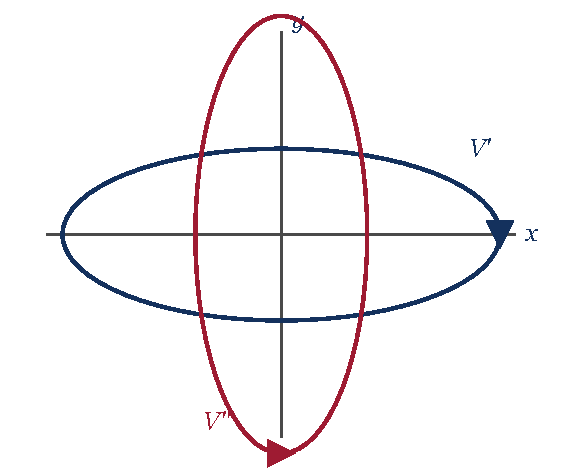
\includegraphics[width=0.5\textwidth]{figuras/pdf/cap06-fig7.pdf}
\caption{Las dos elipses de polarización, iguales y de ejes
perpendiculares, descritas en sentidos contrarios por la molécula
vibrante de los dos rayos refractados en un cristal hemiedro.}
\label{fig:cap6-7}
\end{figure}


% ============================================================
% Capítulo VII — Reflexión (Parte A: §§199-216)
% Traducción de "Théorie mathématique de la lumière" (1889), cap. VII
% Original: §§199-216, páginas impresas 320-358
% Parte A: reflexión vítrea — teorías de Fresnel, de Neumann y
% Mac-Cullagh, y de Cauchy. Continúa en la Parte B (reflexión
% cristalina y metálica), a partir de "Réflexion cristalline".
% ============================================================
\chapter{Reflexión}
\label{cap:reflexion}

\section{Reflexión vítrea}

\noindent La reflexión vítrea ha dado lugar a tres teorías igualmente
confirmadas por la experiencia: son la de Fresnel, la de Neumann y
Mac-Cullagh, y la de Cauchy.

\subsection{Teoría de Fresnel}
\label{sec:reflexion-fresnel}

\subsubsection{Hipótesis fundamentales}

\noindent\textbf{199. Hipótesis fundamentales.} — Fresnel supone:

$1^\circ$ Que la vibración es perpendicular al plano de polarización.

$2^\circ$ Que la elasticidad $\varepsilon$ del éter es constante y es la
misma en los dos medios. La densidad $\rho$ del éter es, por el contrario,
variable. Como la velocidad de propagación $V$ es igual a
$\sqrt{\varepsilon/\rho}$, debemos admitir, si consideramos $\varepsilon$
como constante, que $\rho$ es proporcional al cuadrado del índice de
refracción.

$3^\circ$ Fresnel considera luego las velocidades de dos moléculas
infinitamente vecinas una de otra y de la superficie de separación, pero
situadas a uno y otro lado de esta superficie; descompone cada una de
estas velocidades en otras dos, una paralela al plano tangente a la
superficie de separación, la otra normal a este plano. Admite que las
componentes tangenciales de las velocidades de las dos moléculas deben ser
las mismas en magnitud y dirección, pero que las componentes normales
pueden ser diferentes.\footnote{\emph{Œuvres complètes}, t.~I, p.~767.}

Esta manera de enunciar la hipótesis de la continuidad puede parecer
arbitraria a muchos espíritus. Creemos que es un error. Las vibraciones
del éter son transversales; hemos mostrado (§45) que se puede explicar
esta transversalidad de muchas maneras, pero hemos insistido sobre todo en
dos de esas explicaciones. Se puede suponer que esta transversalidad es el
resultado de una suerte de ligadura, tal que la resistencia del éter a la
compresión sea infinita. Es así, como lo hemos dicho más arriba, la
hipótesis que Fresnel parece haber adoptado en su teoría de la doble
refracción. Aquí adopta la hipótesis contraria, aquella en que las
ecuaciones del movimiento se escriben:
\[
\rho\frac{d^2\xi}{dt^2}=\varepsilon\left(\Delta\xi-\frac{d\Theta}{dx}\right),
\qquad
\rho\frac{d^2\eta}{dt^2}=\varepsilon\left(\Delta\eta-\frac{d\Theta}{dy}\right),
\qquad
\rho\frac{d^2\zeta}{dt^2}=\varepsilon\left(\Delta\zeta-\frac{d\Theta}{dz}\right),
\]
y donde la resistencia del éter a la compresión es nula. Pero, siendo así,
nada impide admitir que las componentes normales de las velocidades de
nuestras dos moléculas infinitamente vecinas sean diferentes. Imaginemos,
en efecto, que la superficie de separación de los dos medios sea un plano
y consideremos dos planos infinitamente vecinos, paralelos al plano de
separación, pero situados de una y otra parte de este plano. Pensemos en
las moléculas de éter situadas en estos dos planos; si las componentes
normales de sus velocidades no son las mismas, la distancia de estos dos
planos variará de manera periódica y resultarán de ello compresiones y
dilataciones alternativas del éter comprendido entre estos dos planos.
Pero, siendo nula la resistencia del éter a la compresión, estas
alternativas podrán producirse sin aportar al movimiento ninguna
perturbación.

$4^\circ$ Finalmente, Fresnel se apoya en el principio de las fuerzas
vivas.

\subsubsection{Aplicación de los principios anteriores}

\noindent\textbf{200. Aplicación de los principios anteriores.} —
Supondremos que la superficie de separación de los dos medios es un plano;
que las ondas incidente, reflejada y refractada son planas. Supondremos
además que el rayo incidente, y por consiguiente los rayos reflejado y
refractado, están enteramente polarizados. Las leyes de la reflexión de la
luz natural se deducen en efecto fácilmente de las de la luz polarizada,
si se considera un rayo natural como la superposición de dos rayos de
igual intensidad polarizados en ángulo recto.

Tomaremos el plano de separación de los dos medios como plano de las
$xy$. Sean $\xi,\eta,\zeta$ las tres componentes del desplazamiento de una
molécula cualquiera; $\xi_1,\eta_1,\zeta_1$ las componentes del
desplazamiento debido a la luz incidente; $\xi_2,\eta_2,\zeta_2$ las del
desplazamiento debido a la luz reflejada; $\xi_3,\eta_3,\zeta_3$ las del
desplazamiento debido a la luz refractada. Tendremos entonces, en el
primer medio,
\[
\xi=\xi_1+\xi_2,\qquad \eta=\eta_1+\eta_2,\qquad \zeta=\zeta_1+\zeta_2,
\]
y en el segundo medio:
\[
\xi=\xi_3,\qquad \eta=\eta_3,\qquad \zeta=\zeta_3.
\]
Según la tercera hipótesis de Fresnel, $\xi$ y $\eta$ son funciones
continuas, pero $\zeta$ puede ser discontinua. Se tiene, pues, para
$z=0$,
\begin{equation}
\xi_1+\xi_2=\xi_3,\qquad \eta_1+\eta_2=\eta_3.
\end{equation}

Siendo planas las ondas, tendremos
\[
\xi_1=A_1\cos(P_1+\omega_1),\qquad \eta_1=B_1\cos(P_1+\omega_1'),\qquad
\zeta_1=C_1\cos(P_1+\omega_1'');
\]
o bien
\[
P_1=\frac{2\pi}{\lambda_1}(\alpha_1x+\beta_1y+\gamma_1z-Vt);
\]
\[
\xi_2=A_2\cos(P_2+\omega_2),\qquad \eta_2=B_2\cos(P_2+\omega_2'),\qquad
\zeta_2=C_2\cos(P_2+\omega_2'');
\]
o bien
\[
P_2=\frac{2\pi}{\lambda_2}(\alpha_2x+\beta_2y+\gamma_2z-Vt);
\]
\[
\xi_3=A_3\cos(P_3+\omega_3),\qquad \eta_3=B_3\cos(P_3+\omega_3'),\qquad
\zeta_3=C_3\cos(P_3+\omega_3'');
\]
o bien
\[
P_3=\frac{2\pi}{\lambda_3}(\alpha_3x+\beta_3y+\gamma_3z-V't).
\]

Las $A$, las $B$ y las $C$, y las $\omega$, son constantes; $V$ tiene el
mismo valor para el rayo incidente y para el rayo reflejado, pues es la
velocidad de propagación en el primer medio; $V'$ es la velocidad de
propagación en el segundo medio, y se tiene, llamando $n$ al índice de
refracción,
\[
V'=\frac{V}{n}.
\]

Debiendo estar las vibraciones en el plano de la onda, tendremos
\begin{equation}
\alpha_1\xi_1+\beta_1\eta_1+\gamma_1\zeta_1
=\alpha_2\xi_2+\beta_2\eta_2+\gamma_2\zeta_2
=\alpha_3\xi_3+\beta_3\eta_3+\gamma_3\zeta_3=0.
\end{equation}

La primera de las ecuaciones (1), que debe ser verificada para $z=0$, nos
da
\begin{align}
&A_1\cos\!\left[\frac{2\pi}{\lambda_1}(\alpha_1x+\beta_1y-Vt)+\omega_1\right]
+A_2\cos\!\left[\frac{2\pi}{\lambda_2}(\alpha_2x+\beta_2y-Vt)+\omega_2\right]
\notag\\
&\hspace{3cm}=A_3\cos\!\left[\frac{2\pi}{\lambda_3}(\alpha_3x+\beta_3y-V't)+\omega_3\right].
\end{align}

\noindent\textbf{201.} Fresnel introduce aquí una hipótesis nueva; es que
$\omega_1=\omega_2$; esta hipótesis no le es sugerida por puntos de vista
teóricos, sino por la experiencia, que le prueba que, mientras no haya
reflexión total, la luz reflejada permanece polarizada rectilíneamente si
la luz incidente lo está ella misma.

En este caso la ecuación (3) no puede verificarse idénticamente más que si
se tiene
\begin{equation}
\frac{\alpha_1}{\lambda_1}=\frac{\alpha_2}{\lambda_2}=\frac{\alpha_3}{\lambda_3},
\qquad
\frac{\beta_1}{\lambda_1}=\frac{\beta_2}{\lambda_2}=\frac{\beta_3}{\lambda_3},
\qquad
\frac{V}{\lambda_1}=\frac{V}{\lambda_2}=\frac{V'}{\lambda_3},
\end{equation}
\[
\omega_1=\omega_2=\omega_3,
\qquad A_1+A_2=A_3.
\]
La segunda ecuación (1) nos daría de la misma manera
\[
\omega_1'=\omega_2'=\omega_3',\qquad B_1+B_2=B_3.
\]

Las ecuaciones (4) nos dan
\[
\lambda_1=\lambda_2,\qquad \alpha_1=\alpha_2,\qquad \beta_1=\beta_2,
\qquad \lambda_3=\frac{\lambda_1}{n},\qquad \alpha_3=\frac{\alpha_1}{n},
\qquad \beta_3=\frac{\beta_1}{n}.
\]

Supondremos que el plano de incidencia haya sido elegido como plano de
las $xz$; tendremos entonces $\beta_1=0$ y, llamando $i$ al ángulo de
incidencia:
\[
\alpha_1=\sin i,\qquad \gamma_1=\cos i.
\]
Si $\beta_1$ es nulo, deberá serlo también $\beta_2$ y $\beta_3$, en
virtud de las ecuaciones (4). Esto significa que la onda reflejada y la
onda refractada son perpendiculares al plano de las $xz$, o en otros
términos que el rayo reflejado y el rayo refractado están en el plano de
incidencia.

Puesto que $\alpha_1=\alpha_2$, tendremos también
\[
\alpha_2=\sin i
\]
y
\[
\gamma_2=\pm\sqrt{1-\alpha_2^2-\beta_2^2}=\pm\cos i.
\]
Como $\gamma_2$ no puede ser igual a $\gamma_1$ sin que el rayo incidente
y el reflejado se confundan, tendremos
\[
\gamma_2=-\gamma_1=-\cos i.
\]
Esto muestra que el ángulo de reflexión es igual al ángulo de incidencia.

De la misma manera, si $r$ es el ángulo de refracción, tendremos
\[
\alpha_3=\sin r,\qquad \gamma_3=\cos r,
\]
y puesto que $\alpha_1=n\alpha_3$, se llega a la ley conocida de la
refracción
\[
\sin i=n\sin r.
\]

La teoría de Fresnel conduce, pues, muy simplemente a las leyes
elementales de la reflexión y de la refracción.

Por otra parte, las ecuaciones (2) se convierten en
\[
A_1\alpha_1\cos(P_1+\omega_1)+C_1\gamma_1\cos(P_1+\omega_1'')=0,
\]
\[
A_2\alpha_2\cos(P_2+\omega_2)+C_2\gamma_2\cos(P_2+\omega_2'')=0,
\]
\[
A_3\alpha_3\cos(P_3+\omega_3)+C_3\gamma_3\cos(P_3+\omega_3'')=0.
\]
Estas ecuaciones no pueden verificarse idénticamente más que si se tiene
\[
A_1\alpha_1+C_1\gamma_1=A_2\alpha_2+C_2\gamma_2=A_3\alpha_3+C_3\gamma_3=0
\]
\[
\omega_1=\omega_1'',\qquad \omega_2=\omega_2'',\qquad \omega_3=\omega_3''.
\]

Si el rayo incidente está polarizado rectilíneamente, tendremos
$\omega_1=\omega_1'$; de modo que las nueve cantidades $\omega$ serán
iguales; podremos entonces suponer que el origen de los tiempos ha sido
elegido de tal manera que estas nueve cantidades sean nulas. Nos quedarán,
pues, entre las cantidades $A$, $B$ y $C$, las relaciones:
\begin{equation}
A_1+A_2=A_3,\qquad B_1+B_2=B_3,
\end{equation}
\begin{equation}
A_1\alpha_1+C_1\gamma_1=0,\qquad A_2\alpha_1-C_2\gamma_1=0,\qquad
A_3\alpha_3+C_3\gamma_3=0.
\end{equation}

\subsubsection{Aplicación del principio de las fuerzas vivas}

\noindent\textbf{202. Aplicación del principio de las fuerzas vivas.} —
Para poder aplicar el principio de las fuerzas vivas, es necesario suponer
que solo una porción del éter está perturbada; pues si todo el espacio
estuviera iluminado, la fuerza viva total sería infinita y la aplicación
del principio se volvería ilusoria.

Supondremos que, en el origen de los tiempos, el éter perturbado se
encuentra encerrado en un paralelepípedo rectangular $CDEF$
(figura~\ref{fig:cap7-1}) limitado por dos planos paralelos al plano de
incidencia, por dos planos paralelos al plano de la onda incidente y por
dos planos perpendiculares a los cuatro primeros. Supondremos además que
las dimensiones de este paralelepípedo sean muy grandes respecto a una
longitud de onda, de manera que no haya que tener en cuenta los fenómenos
de difracción.

\begin{figure}[h]
\centering
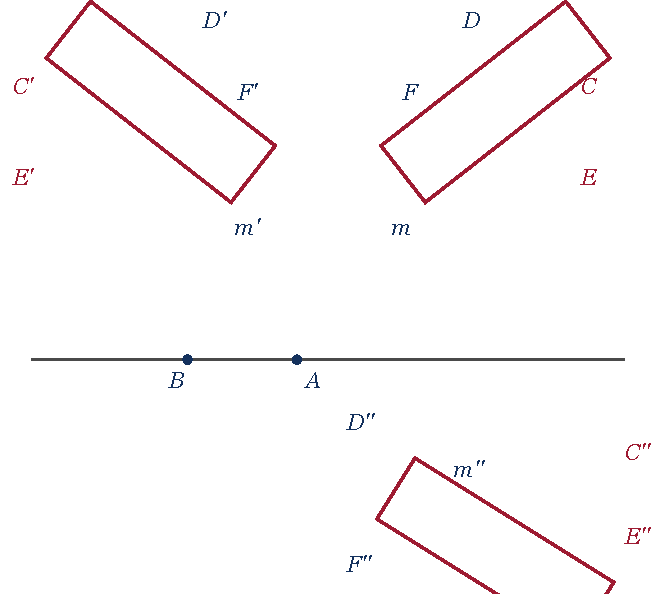
\includegraphics[width=0.85\textwidth]{figuras/pdf/cap07-fig1.pdf}
\caption{El paralelepípedo de éter perturbado $CDEF$ se divide, al cabo
del tiempo $t$, en un paralelepípedo reflejado $C'D'E'F'$ y uno
refractado $C''D''E''F''$.}
\label{fig:cap7-1}
\end{figure}

¿En qué se convertirá la perturbación del éter al cabo de un tiempo $t$?
La perturbación partida de un punto $m$ del paralelepípedo $CDEF$ caminará
primero en la dirección del rayo incidente hasta su encuentro en $\mu$ con
el plano de separación; allí se dividirá en dos partes, una irá de $\mu$ a
$m'$ siguiendo el rayo reflejado, la otra de $\mu$ a $m''$ siguiendo el
rayo refractado. Caminará además con una velocidad $V$ a lo largo de
$m\mu$ y de $\mu m'$ y con una velocidad $V'$ a lo largo de $\mu m''$, de
modo que se deberá tener
\[
\frac{m\mu}{V}+\frac{\mu m'}{V}=\frac{m\mu}{V}+\frac{\mu m''}{V'}=t,
\]
o bien
\begin{equation}
n\cdot\mu m''=\mu m'.
\end{equation}

Así, al tiempo $t$, la luz partida del paralelepípedo $CDEF$ ocupará dos
paralelepípedos: el primero, $C'D'E'F'$, ocupado por la luz reflejada,
tendrá dos caras paralelas al plano de incidencia y dos caras paralelas a
la onda reflejada. El segundo, $C''D''E''F''$, ocupado por la luz
refractada, tendrá dos caras paralelas al plano de incidencia y dos caras
paralelas a la onda refractada. En la figura estos tres paralelepípedos
están representados tomando como plano del dibujo el plano de incidencia.

Sean $q_1,q_2,q_3$ las masas de éter contenidas en estos tres
paralelepípedos. El valor medio de la energía de una masa de éter
perturbada, por ejemplo por la luz incidente, será proporcional, por una
parte, a esta masa, por otra parte a $A_1^2+B_1^2+C_1^2$; el teorema de
las fuerzas vivas se escribirá, pues:
\[
q_1(A_1^2+B_1^2+C_1^2)=q_2(A_2^2+B_2^2+C_2^2)+q_3(A_3^2+B_3^2+C_3^2).
\]

Es claro que $q_1=q_2$; hay que buscar la razón de $q_3$ a $q_1$. Los
volúmenes de nuestros paralelepípedos estarán entre ellos como sus
secciones hechas por el plano de incidencia, es decir, como los
rectángulos $CDEF$, $C''D''E''F''$. Como por otra parte la densidad en el
segundo medio es $n^2$ veces mayor que en el primero, tendremos
\[
\frac{q_3}{q_1}=n^2\,\frac{C''E''}{CE}\cdot\frac{C''D''}{CD}.
\]

Se tiene, en virtud de la ecuación (7):
\[
\frac{C''A}{C'A}=\frac{1}{n},\qquad \frac{E''A}{E'A}=\frac{1}{n},
\]
de donde
\[
C''E''=\frac{1}{n}C'E'=\frac{1}{n}CE.
\]
Por otra parte,
\[
C''D''=AB\cos r,\qquad CD=AB\cos i,
\]
de donde
\[
\frac{q_3}{q_1}=n\,\frac{\cos r}{\cos i}
=\frac{\sin i\cos r}{\sin r\cos i}=\frac{\alpha_1}{\gamma_1}\,\frac{\gamma_3}{\alpha_3}.
\]

El principio de las fuerzas vivas puede entonces escribirse
\[
\frac{\gamma_1}{\alpha_1}(A_1^2+B_1^2+C_1^2-A_2^2-B_2^2-C_2^2)
=\frac{\gamma_3}{\alpha_3}(A_3^2+B_3^2+C_3^2).
\]

Podemos descomponer el rayo incidente en otros dos, uno polarizado en el
plano de incidencia, el otro perpendicularmente a este plano.

Para el primero, $A_1,C_1,A_2,C_2,A_3,C_3$ son nulos.

Para el segundo, $B_1,B_2$ y $B_3$ son nulos.

El principio de las fuerzas vivas debe ser cierto para cada uno de estos
rayos por separado, de modo que la ecuación de las fuerzas vivas se
descompone en dos:
\begin{equation}
\frac{\gamma_1}{\alpha_1}(B_1^2-B_2^2)=\frac{\gamma_3}{\alpha_3}B_3^2,
\end{equation}
\begin{equation}
\frac{\gamma_1}{\alpha_1}(A_1^2-A_2^2+C_1^2-C_2^2)
=\frac{\gamma_3}{\alpha_3}(A_3^2+C_3^2).
\end{equation}

Las ecuaciones (5), (6), (8) y (9) bastan para determinar $A_2,B_2,C_2$ y
$A_3,B_3,C_3$ cuando se conocen $A_1,B_1$ y $C_1$.

\subsubsection{Primeras consecuencias}

\noindent\textbf{203. Primeras consecuencias.} — Si dividimos la ecuación
(8) por la segunda de las ecuaciones (5), resulta:
\begin{equation}
\frac{\gamma_1}{\alpha_1}(B_1-B_2)=\frac{\gamma_3}{\alpha_3}B_3.
\end{equation}

Si en la ecuación (9) reemplazamos $C_1$, $C_2$ y $C_3$ por sus valores
tomados de (6), resulta
\[
\frac{\gamma_1}{\alpha_1}\left(1+\frac{\alpha_1^2}{\gamma_1^2}\right)(A_1^2-A_2^2)
=\frac{\gamma_3}{\alpha_3}\left(1+\frac{\alpha_3^2}{\gamma_3^2}\right)A_3^2,
\]
o dividiendo por la primera ecuación (5),
\[
\frac{\gamma_1}{\alpha_1}\left(1+\frac{\alpha_1^2}{\gamma_1^2}\right)(A_1-A_2)
=\frac{\gamma_3}{\alpha_3}\left(1+\frac{\alpha_3^2}{\gamma_3^2}\right)A_3,
\]
o bien
\begin{equation}
\frac{A_1-A_2}{\alpha_1\gamma_1}=\frac{A_3}{\alpha_3\gamma_3}.
\end{equation}

Las dos ecuaciones (8) y (9) pueden, pues, ser reemplazadas por las
ecuaciones (10) y (11), que tienen la ventaja de ser lineales.

La ecuación (10) puede escribirse (si se recuerda que
$\gamma_2=-\gamma_1$, $\lambda_2=\lambda_1$, $\alpha_1/\lambda_1=\alpha_3/\lambda_3$):
\begin{equation}
\frac{B_1\gamma_1}{\lambda_1}+\frac{B_2\gamma_2}{\lambda_2}
=\frac{B_3\gamma_3}{\lambda_3}.
\end{equation}

De la misma manera la ecuación (11) puede escribirse
\[
A_1\left(\frac{\gamma_1}{\alpha_1}+\frac{\alpha_1}{\gamma_1}\right)
+A_2\left(\frac{\gamma_2}{\alpha_2}+\frac{\alpha_2}{\gamma_2}\right)
=A_3\left(\frac{\gamma_3}{\alpha_3}+\frac{\alpha_3}{\gamma_3}\right),
\]
o teniendo en cuenta las ecuaciones (6)
\[
\frac{A_1\gamma_1-C_1\alpha_1}{\alpha_1}
+\frac{A_2\gamma_2-C_2\alpha_2}{\alpha_2}
=\frac{A_3\gamma_3-C_3\alpha_3}{\alpha_3}.
\]

Esta ecuación y la ecuación (12) se escribirán más simétricamente (al
recordar que los $\beta$ son nulos)
\begin{align}
\frac{B_1\gamma_1-C_1\beta_1}{\lambda_1}
+\frac{B_2\gamma_2-C_2\beta_2}{\lambda_2}
&=\frac{B_3\gamma_3-C_3\beta_3}{\lambda_3},\notag\\
\frac{C_1\alpha_1-A_1\gamma_1}{\lambda_1}
+\frac{C_2\alpha_2-A_2\gamma_2}{\lambda_2}
&=\frac{C_3\alpha_3-A_3\gamma_3}{\lambda_3},
\end{align}
a las cuales se puede añadir la siguiente:
\[
\frac{A_1\beta_1-B_1\alpha_1}{\lambda_1}
+\frac{A_2\beta_2-B_2\alpha_2}{\lambda_2}
=\frac{A_3\beta_3-B_3\alpha_3}{\lambda_3},
\]
que se deduce de la segunda ecuación (5) observando que los $\beta$ son
nulos y que $\alpha_1/\lambda_1=\alpha_2/\lambda_2=\alpha_3/\lambda_3$.

Bajo esta forma simétrica es fácil ver cuál es el significado de las
ecuaciones (13). Tenemos, en efecto, recordando que las cantidades que
habíamos llamado $\omega$ son nulas,
\[
\xi_1=A_1\cos P_1,\qquad \zeta_1=C_1\cos P_1;
\]
de donde
\[
\frac{d\xi_1}{dz}=-\frac{2\pi\gamma_1}{\lambda_1}A_1\sin P_1,
\qquad
\frac{d\zeta_1}{dx}=-\frac{2\pi\alpha_1}{\lambda_1}C_1\sin P_1,
\]
de manera que:
\[
\frac{d\xi_1}{dz}-\frac{d\zeta_1}{dx}=2\pi\sin P_1\,\frac{C_1\alpha_1-A_1\gamma_1}{\lambda_1}.
\]
Así, la segunda ecuación (13) puede escribirse:
\[
\frac{d\xi_1}{dz}-\frac{d\zeta_1}{dx}+\frac{d\xi_2}{dz}-\frac{d\zeta_2}{dx}
=\frac{d\xi_3}{dz}-\frac{d\zeta_3}{dx}.
\]
Ella significa que $\dfrac{d\xi}{dz}-\dfrac{d\zeta}{dx}$ es una función
continua. De la misma manera las otras dos ecuaciones (13) significan que
$\dfrac{d\eta}{dx}-\dfrac{d\xi}{dy}$ y $\dfrac{d\zeta}{dy}-\dfrac{d\eta}{dz}$
son funciones continuas. Estas condiciones pueden reemplazar el principio
de las fuerzas vivas.

Digo que $\dfrac{d\zeta}{dz}$ es también una función continua. En efecto,
$\xi$ y $\eta$ son continuas y es fácil ver que lo mismo ocurre con
$\dfrac{d\xi}{dx}$ y $\dfrac{d\eta}{dy}$. Pero, a causa de la
transversalidad de las vibraciones, se debe tener en los dos medios
\[
\Theta=\frac{d\xi}{dx}+\frac{d\eta}{dy}+\frac{d\zeta}{dz}=0.
\]
Luego $\dfrac{d\zeta}{dz}$ es también continua.

Así, en las hipótesis de Fresnel, no solamente $\xi$ y $\eta$, sino además
$\dfrac{d\xi}{dz}-\dfrac{d\zeta}{dx}$, $\dfrac{d\eta}{dx}-\dfrac{d\xi}{dy}$,
$\dfrac{d\zeta}{dy}-\dfrac{d\eta}{dz}$ y $\dfrac{d\zeta}{dz}$ son funciones
continuas.

\subsubsection{Teorema de Mac-Cullagh}

\noindent\textbf{204. Teorema de Mac-Cullagh.} — Multipliquemos la segunda
ecuación (5) por $\gamma_1/\alpha_1$ y añadámosla a (10) de manera que
eliminemos $B_2$; vendrá
\begin{equation}
2B_1\frac{\gamma_1}{\alpha_1}-B_3\left(\frac{\gamma_1}{\alpha_1}+\frac{\gamma_3}{\alpha_3}\right)=0.
\end{equation}

Eliminemos de la misma manera $A_2$ entre la primera ecuación (5) y la
ecuación (11); vendrá:
\[
2A_1\left(\frac{\gamma_1}{\alpha_1}+\frac{\alpha_1}{\gamma_1}\right)
-A_3\left(\frac{\gamma_1}{\alpha_1}+\frac{\alpha_1}{\gamma_1}
+\frac{\gamma_3}{\alpha_3}+\frac{\alpha_3}{\gamma_3}\right)=0,
\]
o bien
\begin{align}
2A_1\frac{\gamma_1}{\alpha_1}-A_3\left(\frac{\gamma_1}{\alpha_1}+\frac{\gamma_3}{\alpha_3}\right)
&=-2A_1\frac{\alpha_1}{\gamma_1}+A_3\left(\frac{\alpha_1}{\gamma_1}+\frac{\alpha_3}{\gamma_3}\right)
\notag\\
&=\frac{\alpha_1}{\gamma_1}\left[2C_1\frac{\gamma_1}{\alpha_1}-C_3\left(\frac{\gamma_3}{\alpha_3}+\frac{\gamma_1}{\alpha_1}\right)\right].
\end{align}

La comparación de las ecuaciones (14) y (15) da
\[
\begin{vmatrix}A_1&B_1&C_1\\A_3&B_3&C_3\\\alpha_1&0&\gamma_1\end{vmatrix}=0,
\qquad\text{o más simétricamente}\qquad
\begin{vmatrix}A_1&B_1&C_1\\A_3&B_3&C_3\\\alpha_1&\beta_1&\gamma_1\end{vmatrix}=0.
\]

Esta ecuación prueba que el rayo incidente, la vibración incidente y la
vibración refractada están en un mismo plano.

En otros términos la vibración incidente es, en dirección únicamente, la
proyección de la vibración refractada sobre la onda incidente.

Se demostraría de la misma manera que la vibración reflejada es, en
dirección, la proyección de la vibración refractada sobre la onda
reflejada.

\begin{enunciado}{Teorema de Mac-Cullagh (teoría de Fresnel)}
El rayo incidente, la vibración incidente y la vibración refractada están
en un mismo plano: la vibración incidente es, en dirección, la proyección
de la vibración refractada sobre la onda incidente; y de la misma manera,
la vibración reflejada es, en dirección, la proyección de la vibración
refractada sobre la onda reflejada.
\end{enunciado}

\subsubsection{Ley de Brewster}

\noindent\textbf{205. Ley de Brewster.} — Supongamos que el rayo reflejado
sea perpendicular al rayo refractado, es decir, que la onda reflejada sea
perpendicular a la onda refractada.

Toda recta situada en el plano de la onda refractada se proyectará sobre
el plano de la onda reflejada según la recta de intersección de estos dos
planos, es decir, según el eje de las $y$.

Cualquiera que sea, pues, la dirección de la vibración refractada, y por
consiguiente también la dirección de la vibración incidente, la vibración
reflejada será paralela al eje de las $y$.

En otros términos, sea cual sea el plano de polarización del rayo
incidente, el rayo reflejado estará enteramente polarizado en el plano de
incidencia. Será entonces también así cuando la luz incidente sea
natural.

\begin{enunciado}{Ley de Brewster}
Cuando el rayo reflejado es perpendicular al rayo refractado, el rayo
reflejado está enteramente polarizado en el plano de incidencia,
cualquiera que sea el estado de polarización —o la ausencia de ella— del
rayo incidente.
\end{enunciado}

\subsubsection{Reflexión total}

\noindent\textbf{206. Reflexión total.} — Si el segundo medio es menos
refringente que el primero, $n$ es menor que $1$; puede entonces ocurrir
que $\alpha_3$ sea mayor que $1$ y que, en consecuencia, $\gamma_3$ sea
imaginario.

El ángulo de refracción es entonces imaginario, la luz no puede
transmitirse al segundo medio y se refleja toda ella; se dice entonces que
hay reflexión total. En este caso las fórmulas de Fresnel se vuelven
ilusorias, pues la razón $A_2/A_1$, por ejemplo, es imaginaria. Hemos
visto que en el caso ordinario Fresnel había introducido la hipótesis de
que los dos rayos incidente y reflejado tenían la misma fase y que
$\omega_1=\omega_2$.

En el caso de la reflexión total sus fórmulas le dan para $A_2/A_1$ un
valor imaginario de la forma
\[
\cos\varphi+i\sin\varphi.
\]

Fresnel admite, por una suerte de intuición feliz, que el módulo de esta
expresión imaginaria, es decir $1$, representa el verdadero valor de la
razón $A_2/A_1$ y que el argumento de esta misma expresión, es decir
$\varphi$, representa la diferencia de fase $\omega_2-\omega_1$ que había
supuesto hasta entonces nula.

Se vio evidentemente conducido a esta hipótesis audaz por dos experiencias
anteriores que le habían probado que, si el rayo incidente está
polarizado rectilíneamente, el rayo reflejado, que por lo demás tiene la
misma intensidad, está polarizado elípticamente.

Sea cual fuere, su audacia fue plenamente justificada por la experiencia.

\subsubsection{Objeciones contra la teoría de Fresnel}

\noindent\textbf{207. Objeciones contra la teoría de Fresnel.} — El
análisis que precede ha sido entre las manos de Fresnel un admirable
instrumento de descubrimiento; es desde este punto de vista que hay que
considerarlo sin buscarle un rigor que no podría tener. Los teóricos le
han hecho cierto número de objeciones más o menos serias que debemos
refutar si queremos establecer la perfecta concordancia de la teoría de
las ondulaciones con la experiencia.

$1^\circ$ La restricción aportada al principio de la continuidad en lo que
respecta a las componentes normales parece bastante arbitraria;

$2^\circ$ La hipótesis de $\omega_1=\omega_2$ que hemos introducido más
arriba no parece justificada a primera vista por ninguna razón teórica;

$3^\circ$ La fórmula de la reflexión total, confirmada por la experiencia,
parece debida más bien a un feliz azar que a un razonamiento riguroso;

$4^\circ$ Si la elasticidad del éter es constante, su densidad debe ser
proporcional al cuadrado del índice de refracción, pero como este índice
depende de la longitud de onda, esta fórmula conduce, para la densidad del
éter, a valores diferentes según el color de la luz que se considere;

$5^\circ$ Finalmente la teoría anterior no parece, por una razón análoga,
susceptible de extenderse a los medios cristalizados, puesto que el índice
de refracción no es una constante. Si, pues, la densidad se considera como
una constante, no podría ser proporcional al cuadrado de ese índice.

\subsubsection{Refutación de estas objeciones}

\noindent\textbf{208. Refutación de estas objeciones.} — Vamos a buscar
una exposición distinta de la teoría de Fresnel, sin apartarnos del
pensamiento de su autor, pero poniéndonos al abrigo de estas objeciones.

Escribiremos las ecuaciones del movimiento bajo la forma
\[
\rho\frac{d^2\xi}{dt^2}=\varepsilon\left(\Delta\xi-\frac{d\Theta}{dx}\right),
\qquad
\rho\frac{d^2\eta}{dt^2}=\varepsilon\left(\Delta\eta-\frac{d\Theta}{dy}\right),
\qquad
\rho\frac{d^2\zeta}{dt^2}=\varepsilon\left(\Delta\zeta-\frac{d\Theta}{dz}\right).
\]

Consideraremos $\varepsilon$ como constante y $\rho$ como variable;
podremos entonces elegir las unidades de manera que $\varepsilon=1$.
Imaginaremos luego que el espacio se reparte en tres regiones; una
ocupada por el primer medio, y donde $\rho$ podrá considerarse como
constante; otra ocupada por el segundo medio y donde $\rho$ tendrá un
valor constante diferente del de la primera; finalmente entre estas dos
regiones se extenderá una tercera región intermedia, que llamaremos
\emph{capa de paso}, y donde $\rho$ variará muy rápidamente desde su
primer valor constante hasta el segundo. El espesor de esta capa de paso
será finito, pero muy pequeño respecto a una longitud de onda.

Si la superficie de separación es el plano de las $xy$, la capa de paso
estará limitada por dos planos extremadamente vecinos, $z=0$, $z=h$,
paralelos al plano de separación.

Entonces la densidad $\rho$ es una función de $z$ solamente, que
permanece constante de $z=-\infty$ a $z=0$, varía muy rápidamente de $z=0$
a $z=h$ y toma de nuevo un valor constante diferente del primero, de
$z=h$ a $z=+\infty$.

La existencia de semejante capa de paso parecerá más natural que la
hipótesis de un cambio brusco en la naturaleza del medio; nos libra,
además, de todas las dificultades relativas al principio de la
continuidad.

Esto sentado, busquemos satisfacer las ecuaciones del movimiento haciendo:
\[
\xi=\mathrm{X}e^{i(ax+bt)},\qquad \eta=\mathrm{Y}e^{i(ax+bt)},\qquad
\zeta=\mathrm{Z}e^{i(ax+bt)},
\]
siendo X, Y y Z funciones imaginarias de $z$ solamente. Entonces
$\xi,\eta,\zeta$ serán también funciones imaginarias cuyas partes reales
representarán los verdaderos desplazamientos de las moléculas de éter,
conforme a la convención hecha más arriba. Las ecuaciones del movimiento
se convierten entonces en
\[
-\rho b^2\mathrm{X}=\mathrm{X}''-ia\mathrm{Z}',\qquad
-\rho b^2\mathrm{Y}=-a^2\mathrm{Y}+\mathrm{Y}'',\qquad
-\rho b^2\mathrm{Z}=-a^2\mathrm{Z}-ia\mathrm{X}',
\]
representando por letras acentuadas las derivadas de X, Y, Z respecto de
$z$.

En cada uno de los dos medios la densidad $\rho$ es constante y se
encuentra, para la integral de estas ecuaciones,
\[
\mathrm{X}=\mathrm{A}e^{iz\sqrt{\rho b^2-a^2}}+\mathrm{A}'e^{-iz\sqrt{\rho b^2-a^2}},
\]
\[
\mathrm{Y}=\mathrm{B}e^{iz\sqrt{\rho b^2-a^2}}+\mathrm{B}'e^{-iz\sqrt{\rho b^2-a^2}},
\]
\[
\mathrm{Z}=\mathrm{C}e^{iz\sqrt{\rho b^2-a^2}}+\mathrm{C}'e^{-iz\sqrt{\rho b^2-a^2}}.
\]
Llamemos $c$ al valor de $\sqrt{\rho b^2-a^2}$ en el primer medio y $c'$
al valor de este mismo radical en el segundo medio.

Tendremos entonces, comparando nuestras notaciones con las que hemos
empleado más arriba:\footnote{En la última de estas igualdades el
original imprime $\gamma$ en lugar de $b$; se trata de una errata
evidente, pues $b$ es el coeficiente de $t$ en el exponente $i(ax+bt)$.}
\[
a=\frac{2\pi\alpha_1}{\lambda_1}=\frac{2\pi\alpha_2}{\lambda_2}=\frac{2\pi\alpha_3}{\lambda_3},
\qquad
c=\frac{2\pi\gamma_1}{\lambda_1},\qquad c'=\frac{2\pi\gamma_3}{\lambda_3},
\]
\[
b=-\frac{2\pi V}{\lambda_1}=-\frac{2\pi V'}{\lambda_3}.
\]

La expresión de X que acabamos de hallar se compone de dos términos; en el
primer medio, el término en $e^{icz}$ corresponde al rayo incidente y el
término en $e^{-icz}$ corresponde al rayo reflejado; en el segundo medio
el término en $e^{ic'z}$ corresponderá al rayo refractado; el término en
$e^{-ic'z}$ no corresponderá a nada y su coeficiente deberá ser nulo. En
el primer medio tendremos, pues,
\[
\mathrm{X}=\mathrm{A}e^{icz}+\mathrm{A}'e^{-icz},\qquad
\mathrm{Y}=\mathrm{B}e^{icz}+\mathrm{B}'e^{-icz},\qquad
\mathrm{Z}=\mathrm{C}e^{icz}+\mathrm{C}'e^{-icz},
\]
y en el segundo medio
\[
\mathrm{X}=\mathrm{A}''e^{ic'z},\qquad \mathrm{Y}=\mathrm{B}''e^{ic'z},\qquad
\mathrm{Z}=\mathrm{C}''e^{ic'z}.
\]

Si comparamos nuestras notaciones actuales con las que hemos empleado más
arriba, encontraremos:
\[
P_1=ax+cz+bt,\qquad P_2=ax-cz+bt,\qquad P_3=ax+c'z+bt.
\]
\[
\mathrm{A}=A_1e^{i\omega_1},\qquad \mathrm{B}=B_1e^{i\omega_1'},\qquad
\mathrm{C}=C_1e^{i\omega_1''}
\]
\[
\mathrm{A}'=A_2e^{i\omega_2},\qquad \mathrm{B}'=B_2e^{i\omega_2'},\qquad
\mathrm{C}'=C_2e^{i\omega_2''}
\]
\[
\mathrm{A}''=A_3e^{i\omega_3},\qquad \mathrm{B}''=B_3e^{i\omega_3'},\qquad
\mathrm{C}''=C_3e^{i\omega_3''}
\]

Si ponemos
\[
\frac{d\zeta}{dy}-\frac{d\eta}{dz}=u,\qquad
\frac{d\xi}{dz}-\frac{d\zeta}{dx}=v,\qquad
\frac{d\eta}{dx}-\frac{d\xi}{dy}=w,
\]
las ecuaciones del movimiento se convierten en
\[
\rho\frac{d^2\xi}{dt^2}=\frac{dv}{dz}-\frac{dw}{dy},\qquad
\rho\frac{d^2\eta}{dt^2}=\frac{dw}{dx}-\frac{du}{dz},\qquad
\rho\frac{d^2\zeta}{dt^2}=\frac{du}{dy}-\frac{dv}{dx},
\]
o bien:
\[
\frac{du}{dz}=ia w+\rho b^2\eta,\qquad \frac{dv}{dz}=-\rho b^2\xi.
\]

Estas ecuaciones muestran que las derivadas $\dfrac{du}{dz}$ y
$\dfrac{dv}{dz}$ son finitas; y como la capa de paso es extremadamente
delgada, los valores de $u$ y $v$ a los dos lados de esta capa serán
extremadamente poco diferentes. Luego $u$ y $v$ son funciones continuas y
por consiguiente finitas.

Se tiene
\[
\frac{d\xi}{dz}=v+ia\zeta,\qquad \frac{d\eta}{dz}=-u.
\]

Así las derivadas de $\xi$ y de $\eta$ son finitas y por consiguiente
$\xi$ y $\eta$ son continuas. Como por otra parte se tiene
\[
w=ia\eta,
\]
se ve que $w$ es también continua.

Si se suman las tres ecuaciones del movimiento, después de haberlas
diferenciado respectivamente respecto de $x$, $y$ y $z$, viene:
\[
\frac{d(\rho\xi)}{dx}+\frac{d(\rho\eta)}{dy}+\frac{d(\rho\zeta)}{dz}=0,
\]
lo que nos da aquí,\footnote{El original imprime
$\dfrac{d(\rho\zeta)}{dz}=ia\rho\xi$; puesto que
$\dfrac{d(\rho\xi)}{dx}=ia\rho\xi$ y $\dfrac{d(\rho\eta)}{dy}=0$, el signo
correcto es negativo. La errata no afecta al razonamiento, que solo
utiliza la finitud de esta derivada.}
\[
\frac{d(\rho\zeta)}{dz}=-ia\rho\xi.
\]

Esto prueba en primer lugar que $\rho\zeta$ es una función continua y,
como $\rho$ es discontinuo, $\zeta$ no podrá ser continuo a menos de ser
nulo.

Además, siendo $\xi$ continuo, resulta de ello que
\[
\frac{1}{\rho}\,\frac{d(\rho\zeta)}{dz}
\]
es continuo. Pero en los dos medios $\rho$ es constante, $d\rho=0$, de
manera que esta expresión se reduce a $\dfrac{d\zeta}{dz}$.

Así, mediante el cálculo riguroso que precede, reencontramos los mismos
resultados a los que una intuición feliz había conducido a Fresnel: las
funciones $\xi,\eta,u,v,w$ y $\dfrac{d\zeta}{dz}$ son continuas, mientras
que $\zeta$ es discontinua.

Al escribir estas condiciones, resulta\footnote{El original rotula este
sistema como ecuación (15), número que ya había empleado en el §204; se
conserva aquí la numeración impresa, pues el texto se remite a él dos
veces como «(15)» (al final de este párrafo y en el §209).}
\begin{equation}
\begin{gathered}
\mathrm{A}+\mathrm{A}'=\mathrm{A}'',\qquad \mathrm{B}+\mathrm{B}'=\mathrm{B}'',\\
\mathrm{A}c-\mathrm{C}a-\mathrm{A}'c-\mathrm{C}'a=\mathrm{A}''c'-\mathrm{C}''a,
\qquad \mathrm{B}c-\mathrm{B}'c=\mathrm{B}''c',
\end{gathered}
\tag{\thechapter.15}
\end{equation}
a las que hay que añadir las condiciones de transversalidad:\footnote{Se
corrigen aquí dos erratas de signo del original, que imprime
$\mathrm{A}c-\mathrm{C}a+\mathrm{A}'c-\mathrm{C}'a=\mathrm{A}''c'-\mathrm{C}''a$
y $\mathrm{A}''a-\mathrm{C}''c'=0$. Como el término reflejado contiene el
factor $e^{-icz}$ y el refractado el factor $e^{ic'z}$, la continuidad de
$v=\dfrac{d\xi}{dz}-\dfrac{d\zeta}{dx}$ exige $-\mathrm{A}'c$ (en
concordancia con la segunda ecuación (13), donde $\gamma_2=-\gamma_1$, y
con $\mathrm{B}c-\mathrm{B}'c=\mathrm{B}''c'$), y la condición
$\Theta=0$ en el segundo medio da $\mathrm{A}''a+\mathrm{C}''c'=0$, que
es la relación $A_3\alpha_3+C_3\gamma_3=0$ de las ecuaciones (6).}
\[
\mathrm{A}a+\mathrm{C}c=\mathrm{A}'a-\mathrm{C}'c=\mathrm{A}''a+\mathrm{C}''c'=0.
\]

Las condiciones (15) bastan para la solución completa del problema. No
hemos hecho, pues, intervenir el principio de las fuerzas vivas; este
principio es sin embargo ciertamente aplicable en el caso que nos ocupa;
en efecto, las ecuaciones del movimiento de las que nos hemos servido son
las mismas que hemos obtenido en el primer capítulo suponiendo la
existencia de una función de las fuerzas; lo cual implica el principio de
las fuerzas vivas.

\noindent\textbf{209. Reflexión total.} — La cantidad
$c=\dfrac{2\pi\gamma_1}{\lambda_1}$, que se refiere al rayo incidente, es
siempre real; la cantidad $c'$ es también siempre real si el primer medio
es menos refringente que el segundo. Pero, si $n<1$, la cantidad $c'$ no
es real más que si el ángulo de incidencia es bastante pequeño. Si el
ángulo de incidencia sobrepasa cierto límite, $c'$ se vuelve imaginario y
hay reflexión total.

Mientras $c'$ es real, las ecuaciones (15) nos dan para las razones de las
cantidades A, B, C, etc. valores reales; esto equivale a decir que tienen
todas el mismo argumento, o que todas las cantidades $\omega$ son iguales
entre ellas. Si se supone que el origen de los tiempos ha sido elegido de
tal manera que $\omega_1$ sea nulo, las nueve $\omega$ serán nulas. Así se
encuentra justificada la hipótesis de Fresnel.

No ocurre lo mismo cuando $c'$ es imaginario y hay reflexión total; las
razones de los coeficientes A, B, C, etc.\ se volverán imaginarias. Se
vería que las razones
\[
\frac{\mathrm{A}'}{\mathrm{A}},\qquad \frac{\mathrm{B}'}{\mathrm{B}},
\qquad \frac{\mathrm{C}'}{\mathrm{C}}
\]
tienen por módulo la unidad, lo que prueba que la intensidad del rayo
reflejado es la misma que la del rayo incidente. Los argumentos de estas
razones representan las diferencias de fase del rayo reflejado y del rayo
incidente. Así un análisis riguroso, que el empleo de las exponenciales
imaginarias ha vuelto muy simple, nos conduce al mismo resultado que la
inducción audaz de Fresnel.

¿Cuáles serán entonces los movimientos del éter en el segundo medio?
Encontraremos por ejemplo:
\[
\eta=\text{parte real de }\mathrm{B}''e^{i(ax+bt+c'z)}.
\]
Como $c'$ es imaginario podremos poner
\[
c'=ih,
\]
de donde, suponiendo que el origen de los tiempos haya sido elegido de
manera que el argumento de $\mathrm{B}''$ sea nulo,
\[
\eta=\mathrm{B}''e^{-hz}\cos(ax+bt).
\]

Reconocemos así que cierta cantidad de luz penetra en el segundo medio y
que, si no es observable, es a causa de la presencia del factor $e^{-hz}$
que decrece muy rápidamente cuando $z$ crece. Resulta de ello que la
intensidad de la luz refractada no es sensible más que a una débil
distancia del plano de separación, distancia del mismo orden de magnitud
que una longitud de onda.

Se ha logrado detectar la presencia de esta luz refractada\footnote{Quincke,
\emph{Pogg. Ann.}} mediante el siguiente artificio. Dos prismas de vidrio
están separados por una lámina de aire extremadamente delgada; esta
lámina está comprendida entre dos caras paralelas AB y A'B', perteneciendo
la una al primer prisma, la otra al segundo. Un rayo luminoso atraviesa el
primer prisma y viene a encontrar la cara AB bajo un ángulo de incidencia
superior al ángulo límite; la luz refractada penetra en la lámina de aire
y, si esta lámina es lo bastante delgada para que la luz alcance la cara
A'B' antes de haberse extinguido, penetra en el segundo prisma y se
comporta luego regularmente, de manera que se puede observar la luz
transmitida a través de los dos prismas y la lámina de aire.

Esta experiencia parece haber sido hecha por Fresnel\footnote{Fresnel
(?) citado por Verdet, \emph{Leçons d'optique physique}, t.~II.}; ha sido
repetida más recientemente y completada por el Sr. Quincke. El fenómeno es
enteramente análogo al de los anillos coloreados; pero no se observan
entonces las vivas coloraciones que presentan ordinariamente las láminas
delgadas. Es fácil darse cuenta de por qué; en efecto, en la teoría
ordinaria de los anillos coloreados, se encuentra que la intensidad de los
rayos cuya longitud de onda es $\lambda$ es proporcional a
$\sin\dfrac{al}{\lambda}$, designando $l$ el espesor de la lámina y $a$ un
coeficiente que depende de la dirección del rayo luminoso. Para ciertos
valores de $\lambda$, este seno se anula, lo que hace desaparecer los
rayos de ciertos colores y produce una viva coloración de la luz. Aquí
$a$ es imaginario y los senos ordinarios son reemplazados por senos
hiperbólicos que no pueden anularse salvo si $l=0$. Las vivas coloraciones
no aparecerán, pues.

No insistiremos sobre esta experiencia; nos limitaremos a añadir que los
resultados concuerdan con la teoría de una manera bastante satisfactoria,
pero que subsisten sin embargo ligeras diferencias que parecen explicarse
porque el espesor de la capa de paso no sería del todo despreciable frente
a una longitud de onda.

\subsubsection{Objeción relativa a la dispersión}

\noindent\textbf{210. Objeción relativa a la dispersión.} — Las
consideraciones que preceden nos parecen refutar completamente las tres
primeras objeciones hechas a la teoría de Fresnel. Volveremos sobre la
quinta a propósito de la reflexión cristalina; pero debemos hablar aquí
de la cuarta, que es relativa a la dispersión. Para refutarla, hay que
remitirse a lo que hemos dicho acerca de las teorías de la dispersión.

Tomemos por ejemplo la última de las teorías que hemos expuesto. En esta
teoría se considera la acción mutua de las moléculas de éter y de las
moléculas materiales, y las ecuaciones del movimiento se escriben, llamando
$\xi,\eta,\zeta$ las componentes del desplazamiento de una molécula de
éter, $\xi_1,\eta_1,\zeta_1$ las del desplazamiento de una molécula
material, $\rho$ la densidad del éter, $\rho_1$ la de la materia, M un
coeficiente bastante grande:
\[
\rho\frac{d^2\xi}{dt^2}=\Delta\xi-\frac{d\Theta}{dx}+\mathrm{M}(\xi_1-\xi),
\qquad
\rho_1\frac{d^2\xi_1}{dt^2}=\mathrm{M}(\xi-\xi_1),
\]
\[
\rho\frac{d^2\eta}{dt^2}=\Delta\eta-\frac{d\Theta}{dy}+\mathrm{M}(\eta_1-\eta),
\qquad
\rho_1\frac{d^2\eta_1}{dt^2}=\mathrm{M}(\eta-\eta_1),
\]
\[
\rho\frac{d^2\zeta}{dt^2}=\Delta\zeta-\frac{d\Theta}{dz}+\mathrm{M}(\zeta_1-\zeta),
\qquad
\rho_1\frac{d^2\zeta_1}{dt^2}=\mathrm{M}(\zeta-\zeta_1).
\]
M, $\rho$ y $\rho_1$ deben considerarse como funciones de $z$ que,
constantes en cada uno de los dos medios, varían muy rápidamente en la
capa de paso.

Supongamos que se busque satisfacer estas ecuaciones haciendo
\[
\xi=\mathrm{X}e^{i(ax+bt)},\qquad \xi_1=\mathrm{X}_1e^{i(ax+bt)},
\]
\[
\eta=\mathrm{Y}e^{i(ax+bt)},\qquad \eta_1=\mathrm{Y}_1e^{i(ax+bt)},
\]
\[
\zeta=\mathrm{Z}e^{i(ax+bt)},\qquad \zeta_1=\mathrm{Z}_1e^{i(ax+bt)};
\]
se tiene entonces
\[
\frac{1}{\xi}\frac{d^2\xi}{dt^2}=\frac{1}{\eta}\frac{d^2\eta}{dt^2}
=\frac{1}{\zeta}\frac{d^2\zeta}{dt^2}=\frac{1}{\xi_1}\frac{d^2\xi_1}{dt^2}
=\cdots=-b^2,
\]
de donde
\[
\rho_1b^2\xi_1+\mathrm{M}(\xi-\xi_1)=0,\qquad \xi_1=\frac{\mathrm{M}\xi}{\mathrm{M}-\rho_1b^2}.
\]
Pongamos
\[
\rho'=\rho+\frac{\mathrm{M}\rho_1}{\mathrm{M}-\rho_1b^2};
\]
resultará, reemplazando $\xi_1$ por su valor en la primera de las
ecuaciones del movimiento,
\[
-\rho'b^2\xi=\Delta\xi-\frac{d\Theta}{dx},
\]
y de la misma manera
\[
-\rho'b^2\eta=\Delta\eta-\frac{d\Theta}{dy},\qquad
-\rho'b^2\zeta=\Delta\zeta-\frac{d\Theta}{dz}.
\]

Todo ocurre, pues, como si cada uno de los dos medios fuera homogéneo y
tuviera por densidad $\rho'$. Pero esta densidad ficticia $\rho'$ depende
de $b$, es decir, de la longitud de onda. Todo ocurre, pues, como si la
densidad del éter no fuera la misma para los diferentes colores, y la
cuarta objeción se encuentra descartada.

La teoría de Briot, que explica la dispersión admitiendo que $\rho$ no es
una constante sino una función periódica, permite también refutar sin
dificultad esta objeción. Esto no sería tan fácil si se admitiera la
teoría de Cauchy.

\subsection{Teoría de Neumann y Mac-Cullagh}
\label{sec:reflexion-neumann}

\noindent\textbf{211.} Neumann y Mac Cullagh han
fundado, sobre hipótesis enteramente contrarias a las de Fresnel, una
teoría que sin embargo también está confirmada por la experiencia. En el
estudio de esta teoría, adoptaremos un modo de exposición que difiere
mucho del de sus inventores, pero que hace resaltar mejor la verdadera
razón de este hecho singular.

Sean $\xi,\eta,\zeta$ las proyecciones sobre los tres ejes del
desplazamiento debido a la propagación de una onda plana cualquiera, de
manera que $\xi,\eta,\zeta$ sean las partes reales de
\[
\mathrm{A}e^{iP},\qquad \mathrm{B}e^{iP},\qquad \mathrm{C}e^{iP},
\]
o bien
\[
P=\frac{2\pi}{\lambda}(\alpha x+\beta y+\gamma z-Vt).
\]
Si ponemos
\[
u=\frac{d\zeta}{dy}-\frac{d\eta}{dz},\qquad v=\frac{d\xi}{dz}-\frac{d\zeta}{dx},
\qquad w=\frac{d\eta}{dx}-\frac{d\xi}{dy};
\]
$u,v,w$ serán las partes reales de
\[
\mathrm{A}'e^{iP},\qquad \mathrm{B}'e^{iP},\qquad \mathrm{C}'e^{iP},
\]
o bien
\[
\mathrm{A}'=\frac{2\pi i}{\lambda}(\beta\mathrm{C}-\gamma\mathrm{B}),\qquad
\mathrm{B}'=\frac{2\pi i}{\lambda}(\gamma\mathrm{A}-\alpha\mathrm{C}),\qquad
\mathrm{C}'=\frac{2\pi i}{\lambda}(\alpha\mathrm{B}-\beta\mathrm{A}).
\]

Si consideramos $u,v,w$ como las proyecciones sobre los tres ejes del
desplazamiento debido a la propagación de una segunda onda plana, habrá
entre los dos movimientos vibratorios representados respectivamente por
$\xi,\eta,\zeta$ y por $u,v,w$ las relaciones siguientes:

$1^\circ$ Las dos vibraciones $(\xi,\eta,\zeta)$ y $(u,v,w)$ estarán ambas
en el plano de la onda (que será el mismo para los dos movimientos
vibratorios); pero serán perpendiculares la una a la otra.

$2^\circ$ Hay entre las dos vibraciones una diferencia de fase igual a
$\pi/2$ (a causa del factor $i$ que entra en A', B' y C').

$3^\circ$ La amplitud de la vibración $(u,v,w)$ estará con la de la
vibración $(\xi,\eta,\zeta)$ en la razón $2\pi/\lambda$.

\noindent\textbf{212.} Volvamos ahora a la teoría de Fresnel que acabamos
de exponer; hemos visto que si llamamos
$\xi_1,\eta_1,\zeta_1;\xi_2,\eta_2,\zeta_2;\xi_3,\eta_3,\zeta_3$ las
componentes del desplazamiento debido respectivamente a la luz incidente,
a la luz reflejada y a la luz refractada, consideraciones teóricas
condujeron a Fresnel a establecer entre estas nueve cantidades ciertas
relaciones que la experiencia ha confirmado.

Se pueden formar entonces las cantidades $u_1,v_1,w_1;u_2,v_2,w_2;
u_3,v_3,w_3$ de la manera siguiente:
\[
u_1=\frac{d\zeta_1}{dy}-\frac{d\eta_1}{dz},\quad\ldots
\qquad
u_2=\frac{d\zeta_2}{dy}-\frac{d\eta_2}{dz},\quad\ldots
\]

Supongamos con Neumann y Mac Cullagh que la vibración es paralela al
plano de polarización, perpendicular por consiguiente a la vibración de
Fresnel.

Supongamos al mismo tiempo que las tres componentes de las vibraciones
incidente, reflejada y refractada son respectivamente $u_1,v_1,w_1;
u_2,v_2,w_2;u_3,v_3,w_3$, estando estas cantidades ligadas por las mismas
relaciones que en la teoría de Fresnel.

Vamos a mostrar primero que estas hipótesis no son contradichas por la
experiencia, es decir que los resultados verificables experimentalmente
son los mismos que en la teoría de Fresnel.

En efecto, las vibraciones $(\xi,\eta,\zeta)$ y $(u,v,w)$ son
perpendiculares entre ellas, de donde se sigue que la dirección de las
vibraciones incidente, reflejada y refractada es en la teoría de Neumann
perpendicular a lo que es en la teoría de Fresnel; pero, como suponemos al
mismo tiempo que el plano de polarización es paralelo a la vibración y no
perpendicular como lo imaginaba Fresnel, el plano de polarización, que es
lo único accesible a la experiencia, es el mismo en las dos teorías
opuestas.

Sean $\mathrm{I}_1,\mathrm{I}_2,\mathrm{I}_3$ las intensidades de las
luces incidente, reflejada y refractada en la teoría de Fresnel; sean
$\mathrm{I}_1',\mathrm{I}_2',\mathrm{I}_3'$ las intensidades de estas
mismas luces en la teoría de Neumann. Sean $\lambda_1,\lambda_2,\lambda_3$
las longitudes de onda correspondientes.

Como las intensidades son proporcionales a los cuadrados de las
amplitudes, tendremos
\[
\mathrm{I}_1'=\frac{4\pi^2}{\lambda_1^2}\mathrm{I}_1,\qquad
\mathrm{I}_2'=\frac{4\pi^2}{\lambda_2^2}\mathrm{I}_2,\qquad
\mathrm{I}_3'=\frac{4\pi^2}{\lambda_3^2}\mathrm{I}_3.
\]
Como $\lambda_1=\lambda_2=n\lambda_3$ tendremos
\[
\frac{\mathrm{I}_2'}{\mathrm{I}_1'}=\frac{\mathrm{I}_2}{\mathrm{I}_1},\qquad
\frac{\mathrm{I}_3'}{\mathrm{I}_1'}=n^2\frac{\mathrm{I}_3}{\mathrm{I}_1}.
\]

Así la razón de la intensidad de la luz reflejada a la de la luz incidente
es la misma en las dos teorías, de manera que las experiencias que
determinan esta razón no permiten tampoco decidir entre ellas.

La razón $\mathrm{I}_3'/\mathrm{I}_1'$ es por el contrario diferente de la
razón $\mathrm{I}_3/\mathrm{I}_1$; pero si suponemos por ejemplo que el
primer medio sea el aire y el segundo el vidrio, se podrá observar la
intensidad de la luz incidente, pero no se tendrá ningún medio de observar
en el vidrio la de la luz refractada; habrá que esperar, para que esta
observación sea posible, que esta luz haya salido del vidrio por una
nueva refracción para penetrar de nuevo en el aire. Su intensidad se
habrá vuelto entonces $\mathrm{I}_4$ en la teoría de Fresnel,
$\mathrm{I}_4'$ en la de Neumann y, puesto que la longitud de onda será de
nuevo igual a $\lambda_1$ (longitud de onda en el aire), tendremos:
\[
\mathrm{I}_4'=\frac{4\pi^2}{\lambda_1^2}\mathrm{I}_4,
\]
de modo que vendrá aún
\[
\frac{\mathrm{I}_4'}{\mathrm{I}_1'}=\frac{\mathrm{I}_4}{\mathrm{I}_1}.
\]

De la misma manera las experiencias de interferencia, tales como la de
los tres espejos, no pueden permitir dar la preferencia a una de las dos
teorías. Si dos rayos interfieren de manera que se destruyan es porque los
valores de $\xi,\eta,\zeta$ relativos a estos dos rayos son
respectivamente iguales y de signo contrario. Ocurrirá entonces
evidentemente lo mismo con los valores de
\[
u=\frac{d\zeta}{dy}-\frac{d\eta}{dz},\qquad v=\frac{d\xi}{dz}-\frac{d\zeta}{dx},
\qquad w=\frac{d\eta}{dx}-\frac{d\xi}{dy}.
\]

En resumen las dos teorías son ambas igualmente conformes a la
experiencia.

\subsubsection{Principio de continuidad}

\noindent\textbf{213. Principio de continuidad.} — Hemos visto (§203) que
$u,v,w$ son funciones continuas. Como estas funciones representan en la
nueva teoría las componentes del desplazamiento, vemos que estas tres
componentes son continuas. El principio de continuidad no está, pues, ya
sometido aquí a la misma restricción que en la teoría de Fresnel, donde
las componentes paralelas al plano de separación debían ser continuas
mientras que la componente normal podía ser discontinua.

Esta condición de continuidad se expresa escribiendo que, para $z=0$, se
tiene\footnote{A partir de aquí Poincaré reinicia la numeración de las
ecuaciones dentro de la teoría de Neumann y Mac-Cullagh, como ya ha
ocurrido en capítulos anteriores del libro.}
\setcounter{equation}{0}
\begin{equation}
u_1+u_2=u_3;\qquad v_1+v_2=v_3;\qquad w_1+w_2=w_3.
\end{equation}

\subsubsection{Densidad del éter}

\noindent\textbf{214. Densidad del éter.} — Veamos cuál debe ser, en la
nueva teoría, la densidad del éter. Remitámonos a lo que hemos dicho más
arriba a propósito de la aplicación del principio de las fuerzas vivas
(§202). Este principio debe ser aplicable tanto en la hipótesis de
Neumann como en la de Fresnel. Sean $v_1,v_2,v_3$ los volúmenes de tres
paralelepípedos de éter $CDEF$, $C'D'E'F'$ y $C''D''E''F''$. Sean
$\rho_1$ y $\rho_3$ las densidades del éter admitidas por Fresnel en el
primero y el segundo medio; $\rho_1'$ y $\rho_3'$ lo que deben ser estas
mismas densidades en la nueva teoría; se tendrá según una de las
hipótesis de Fresnel
\[
\rho_3=n^2\rho_1.
\]

El principio de las fuerzas vivas se escribirá en la teoría de Fresnel
\begin{equation}
\rho_1(v_1\mathrm{I}_1-v_2\mathrm{I}_2)=\rho_3v_3\mathrm{I}_3,
\end{equation}
y en la de Neumann
\begin{equation}
\rho_1'(v_1\mathrm{I}_1'-v_2\mathrm{I}_2')=\rho_3'v_3\mathrm{I}_3'.
\end{equation}

La ecuación (2) da
\[
v_1\mathrm{I}_1-v_2\mathrm{I}_2=n^2v_3\mathrm{I}_3
\]
de donde
\[
v_1\mathrm{I}_1'-v_2\mathrm{I}_2'=v_3\mathrm{I}_3',
\]
o bien, comparando con (3):
\[
\rho_3'=\rho_1'.
\]

Así en la teoría de Neumann, la densidad del éter debe considerarse como
constante y su elasticidad como la única variable.

En resumen las hipótesis que hemos hecho equivalen a las siguientes, que
son las enunciadas por Neumann y Mac Cullagh:

$1^\circ$ La vibración es paralela al plano de
polarización;\footnote{El original imprime aquí «perpendiculaire», errata
evidente: toda la teoría de Neumann y Mac-Cullagh descansa en la hipótesis
contraria a la de Fresnel (§212), y el propio Poincaré la enuncia como
«La vibration est parallèle au plan de polarisation» en el §217.}

$2^\circ$ La densidad del éter es constante;

$3^\circ$ Las tres componentes del desplazamiento son funciones
continuas.

\subsubsection{Teorema de Mac-Cullagh}

\noindent\textbf{215. Teorema de Mac-Cullagh.} — Sea $O$
(figura~\ref{fig:cap7-2}) un punto del plano de separación; tracemos por
este punto tres rectas $OI$, $OR'$ y $OR$ cuyas proyecciones sobre los
tres ejes sean respectivamente $u_1,v_1,w_1;u_2,v_2,w_2;u_3,v_3,w_3$. Estas
tres rectas representarán, en magnitud y dirección, en la teoría de
Neumann, las vibraciones incidente, reflejada y refractada. Según las
ecuaciones (1), $OR$ es la suma geométrica de $OI$ y $OR'$, es decir, la
diagonal del paralelogramo construido sobre $OI$ y $OR'$. Las tres rectas
$OI$, $OR$ y $OR'$ están, pues, en un mismo plano.

\begin{figure}[h]
\centering
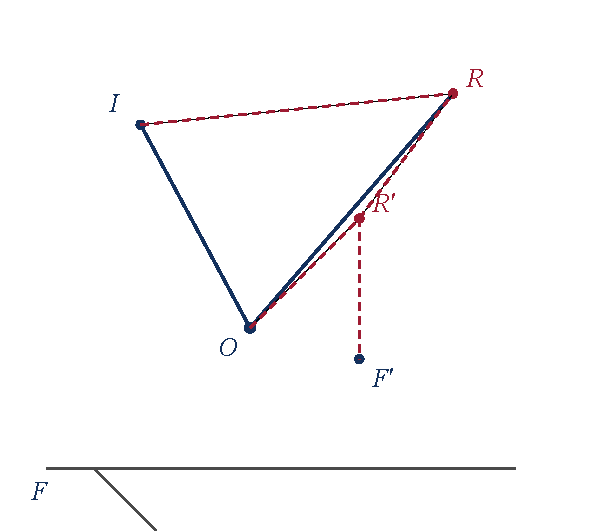
\includegraphics[width=0.75\textwidth]{figuras/pdf/cap07-fig2.pdf}
\caption{Construcción del teorema de Mac-Cullagh: la vibración refractada
$OR$ es la diagonal del paralelogramo construido sobre la vibración
incidente $OI$ y la vibración reflejada $OR'$.}
\label{fig:cap7-2}
\end{figure}

Busquemos determinar este plano. Sean $OF$ y $OF'$ las direcciones de las
vibraciones incidente y refractada en la teoría de Fresnel. El plano
$IOF$ es el de la onda incidente, el plano $ROF'$ el de la onda
refractada.\footnote{El original imprime aquí «le plan R'OF'» y, unas
líneas más abajo, «l'angle IFO»; según la asignación de letras hecha al
comienzo de este párrafo ($OR'$ reflejada, $OR$ refractada) y la
construcción que sigue, debe leerse $ROF'$ e $IOF$, respectivamente.}
Según un teorema demostrado más arriba (§204), $OF$ es la
proyección de $OF'$ sobre la onda incidente; los dos planos $IOF$ y
$F'OF$ son, pues, rectangulares; además el ángulo $IOF$ es recto; luego
$OI$ es perpendicular al plano $FOF'$ y por consiguiente a $OF'$; $OF'$
perpendicular a la vez a $OI$ y a $OR'$ es perpendicular al plano $ROI$.
Luego el plano $ROI$ y el plano de la onda refractada son rectangulares.
Luego \emph{el plano de las tres vibraciones $OI$, $OR$ y $OR'$ pasa por
el rayo refractado.}

Esto permite resolver el siguiente problema: conociendo en magnitud y
dirección la vibración incidente $OI$ (en la teoría de Neumann),
construir las vibraciones reflejada y refractada.

Por $OI$ y el rayo refractado hagamos pasar un plano que corte la onda
reflejada según cierta recta $OR'$ y la onda refractada según una recta
$OR$. Por el punto $I$ tracemos una paralela a $OR'$ hasta su encuentro en
$R$ con $OR$, luego por el punto $R$ una paralela a $OI$ hasta su
encuentro en $R'$ con $OR'$. Hemos construido así en magnitud y dirección
las rectas $OR$ y $OR'$.

Si se quiere enunciar el teorema sin hacer intervenir la dirección de la
vibración, hay que decir:

\begin{enunciado}{Teorema de Mac-Cullagh (teoría de Neumann)}
El plano de polarización del rayo refractado corta el plano de
polarización del rayo incidente según una recta perpendicular al rayo
incidente, y el plano de polarización del rayo reflejado según una recta
perpendicular al rayo reflejado.
\end{enunciado}

\subsection{Teoría de Cauchy}
\label{sec:reflexion-cauchy}

\noindent\textbf{216.}\footnote{\emph{Nouveaux
exercices de mathématiques}, \emph{Comptes rendus}, passim 1836 y 1839.
\emph{Œuvres complètes}, primera serie, t.~IV, passim y principalmente
p.~112 y ss., primera serie, t.~V, p.~111.} Cauchy toma por punto de
partida el principio de continuidad, al cual no aporta ninguna
restricción; no solamente $\xi,\eta$ y $\zeta$ deben ser funciones
continuas, sino que lo mismo ocurre con las derivadas
$\dfrac{d\xi}{dz},\dfrac{d\eta}{dz}$ y $\dfrac{d\zeta}{dz}$ (si se toma
como plano de las $xy$ el plano de separación).

Sería imposible satisfacer estas condiciones si no se admitiera que,
junto a las vibraciones transversales susceptibles de ser observadas, se
propagan igualmente vibraciones longitudinales inaccesibles a la
experiencia. No debemos, pues, admitir que la velocidad de propagación de
los rayos longitudinales sea nula; tampoco puede ser real, pues de lo contrario una
porción de la fuerza viva debida a la luz incidente sería absorbida por
estas ondas longitudinales y la experiencia no indica ningún rastro de
semejante pérdida de fuerza viva.

Nos vemos, pues, conducidos a suponer que esta velocidad de propagación
es imaginaria; será por ejemplo $i\varepsilon$ en el primer medio e
$i\varepsilon'$ en el segundo. Por lo demás $\varepsilon$ y $\varepsilon'$
serán muy pequeños. De esta manera los rayos longitudinales serán
evanescentes (§53) y no absorberán fuerza viva.

Sean $\xi_1,\eta_1,\zeta_1$ las componentes del desplazamiento debido a
las vibraciones transversales, $\xi_2,\eta_2,\zeta_2$ las componentes del
desplazamiento debido a las vibraciones longitudinales, tendremos:
\[
\xi=\xi_1+\xi_2,\qquad \eta=\eta_1+\eta_2,\qquad \zeta=\zeta_1+\zeta_2.
\]

Busquemos satisfacer las condiciones poniendo como más arriba (§210)
\[
\xi_1=\mathrm{X}_1e^{i(ax+bt)},\qquad \eta_1=\mathrm{Y}_1e^{i(ax+bt)},
\qquad \zeta_1=\mathrm{Z}_1e^{i(ax+bt)},
\]
\[
\xi_2=\mathrm{X}_2e^{i(ax+bt)},\qquad \eta_2=\mathrm{Y}_2e^{i(ax+bt)},
\qquad \zeta_2=\mathrm{Z}_2e^{i(ax+bt)},
\]
siendo las X, las Y y las Z funciones de $z$ solamente.

Tendremos, en el primer medio, es decir para $z<0$,
\[
\mathrm{X}_2=\mathrm{A}e^{+hz},\qquad \mathrm{Y}_2=\mathrm{B}e^{+hz},
\qquad \mathrm{Z}_2=\mathrm{C}e^{+hz};
\]
y en el segundo medio, es decir para $z>0$,
\[
\mathrm{X}_2=\mathrm{A}'e^{-h'z},\qquad \mathrm{Y}_2=\mathrm{B}'e^{-h'z},
\qquad \mathrm{Z}_2=\mathrm{C}'e^{-h'z}.
\]

Escribamos que la velocidad de propagación en el primer medio es
$i\varepsilon$, vendrá
\[
\frac{b^2}{a^2-h^2}=-\varepsilon^2\qquad\text{o}\qquad h=\sqrt{a^2+\frac{b^2}{\varepsilon^2}}.
\]
Se encuentra de la misma manera
\[
h'=\sqrt{a^2+\frac{b^2}{\varepsilon'^2}}.
\]

Vemos primero que, siendo $\varepsilon$ y $\varepsilon'$ muy pequeños, $h$
y $h'$ serán muy grandes. Por consiguiente los factores $e^{hz}$ (en el
primer medio donde $z<0$) y $e^{-h'z}$ (en el segundo medio donde $z>0$)
serán muy pequeños a menos que el valor absoluto de $z$ no sea muy
pequeño. No habrá, pues, luz longitudinal sensible más que en la vecindad
inmediata del plano de separación, lo que explica por qué es inobservable
y no absorbe fuerza viva.

Escribamos que la vibración $(\xi_2,\eta_2,\zeta_2)$ es longitudinal;
tendremos:\footnote{Poincaré reinicia aquí la numeración de las
ecuaciones dentro de la teoría de Cauchy, pero el original rotula esta
relación directamente como ecuación (2): ni en el §216 ni en las páginas
que lo preceden desde el comienzo de la teoría de Cauchy figura ninguna
ecuación (1) —un salto de numeración semejante al que ya se documentó en
el Capítulo I (ecuación 37 inexistente) y en el Capítulo IV (ecuación 9
inexistente)—. Se conserva la numeración tal como aparece impresa, pues
el texto se remite después a las «condiciones (2)».}
\setcounter{equation}{1}
\begin{equation}
\frac{d\zeta_2}{dy}-\frac{d\eta_2}{dz}=\frac{d\xi_2}{dz}-\frac{d\zeta_2}{dx}
=\frac{d\eta_2}{dx}-\frac{d\xi_2}{dy}=0.
\end{equation}

Esto muestra que $\dfrac{d\zeta_2}{dy}-\dfrac{d\eta_2}{dz}$ es continuo;
lo es también de
$\dfrac{d\zeta}{dy}-\dfrac{d\eta}{dz}$, puesto que, según el principio de
Cauchy, $\xi,\eta,\zeta$ son continuas así como sus derivadas de primer
orden. Luego
$\dfrac{d\zeta_1}{dy}-\dfrac{d\eta_1}{dz}$ es continuo, de la misma manera
que $\dfrac{d\xi_1}{dz}-\dfrac{d\zeta_1}{dx}$,
$\dfrac{d\eta_1}{dx}-\dfrac{d\xi_1}{dy}$. Así, si no consideramos más que la
luz transversal observable, las cantidades que hemos llamado más arriba
$u,v,w$ son continuas como en la teoría de Fresnel.

Las condiciones (2) pueden también escribirse,
\[
\frac{\mathrm{A}}{a}=\frac{\mathrm{C}}{-ih},\qquad
\frac{\mathrm{A}'}{a}=\frac{\mathrm{C}'}{+ih'},\qquad
\mathrm{B}=\mathrm{B}'=0.
\]
Luego $\eta_2=0$ y, como $\eta$ es continuo, $\eta_1$ deberá serlo también
como en la teoría de Fresnel.

Resulta luego, en el primer medio
\[
h^2\frac{d\xi_2}{dx}+a^2\frac{d\zeta_2}{dz}=0,
\]
y en el segundo medio
\[
h'^2\frac{d\xi_2}{dx}+a^2\frac{d\zeta_2}{dz}=0,
\]
o, lo que es lo mismo, en el primer medio
\begin{equation}
b^2\frac{d\xi_2}{dx}+a^2\varepsilon^2\left(\frac{d\xi_2}{dx}+\frac{d\zeta_2}{dz}\right)=0,
\end{equation}
y en el segundo
\begin{equation}
b^2\frac{d\xi_2}{dx}+a^2\varepsilon'^2\left(\frac{d\xi_2}{dx}+\frac{d\zeta_2}{dz}\right)=0.
\end{equation}

Siendo la vibración $(\xi_1,\eta_1,\zeta_1)$ transversal, tendremos en los
dos medios
\[
\frac{d\xi_1}{dx}+\frac{d\zeta_1}{dz}=0 \qquad (\eta_1 \text{ es
independiente de } y);
\]
y como $\dfrac{d\xi}{dx}+\dfrac{d\zeta}{dz}$ es continuo, esto significa
que $\dfrac{d\xi_2}{dx}+\dfrac{d\zeta_2}{dz}$ es igualmente continuo.

Si llamamos, pues, $\xi_2^0$ y $\zeta_2^0$ los valores de $\xi_2$ y de
$\zeta_2$ en el primer medio, pero infinitamente cerca del plano de
separación, y de la misma manera $\xi_2^1$ y $\zeta_2^1$ los valores de
$\xi_2$ y de $\zeta_2$ en el segundo medio, e infinitamente cerca del
plano de separación, tendremos
\[
\frac{d\xi_2^0}{dx}+\frac{d\zeta_2^0}{dz}=\frac{d\xi_2^1}{dx}+\frac{d\zeta_2^1}{dz};
\]
y las ecuaciones (3) y (4) darán
\begin{equation}
\frac{d\xi_2^1}{dx}-\frac{d\xi_2^0}{dx}
=\frac{a^2}{b^2}(\varepsilon^2-\varepsilon'^2)\left(\frac{d\xi_2^0}{dx}+\frac{d\zeta_2^0}{dz}\right).
\end{equation}

Si la velocidad de propagación de las vibraciones longitudinales fuera la
misma en todos los medios, se tendría $\varepsilon=\varepsilon'$; el
segundo miembro de la igualdad (5) sería nulo y $\dfrac{d\xi_2}{dx}$ sería
continuo.

Resultaría de ello que $\dfrac{d\xi_1}{dx}$ y por consiguiente $\xi_1$
serían funciones continuas y habría concordancia completa con la teoría
de Fresnel.

Pero es más natural suponer $\varepsilon\gtrless\varepsilon'$; en este
caso, como $\varepsilon$ y $\varepsilon'$ son ambos muy pequeños, el
segundo miembro de (5) no es ya nulo sino solamente muy pequeño y la
concordancia con la teoría de Fresnel no es ya más que aproximativa. En
particular el rayo reflejado debería presentar rastros de polarización
elíptica.

La teoría de Cauchy pareció por un instante recibir una confirmación
brillante cuando las experiencias de Jamin revelaron la existencia de
estos rastros de polarización elíptica que el geómetra francés había
previsto. Pero nuevas experiencias del mismo físico cesaron de concordar
con las previsiones de Cauchy.

Sean $i\varepsilon,i\varepsilon',i\varepsilon''$ las velocidades de la luz
longitudinal en el aire, en el agua y en el vidrio; las observaciones de
Jamin sobre la refracción del aire en el vidrio deberían dar la razón
$\varepsilon/\varepsilon''$; de la misma manera observando la refracción
del aire en el agua, luego del agua en el vidrio, se deberían encontrar
las razones $\varepsilon/\varepsilon'$ y $\varepsilon'/\varepsilon''$.

El primer cociente debería ser igual al producto de los otros dos; no es
nada de eso.

Por eso la teoría de Cauchy está hoy abandonada, y se prefiere explicar
los fenómenos observados por Jamin admitiendo que el espesor de la capa
de paso (§208) no es despreciable frente a una longitud de onda.

\section{Reflexión cristalina}
\label{sec:reflexion-cristalina}

Hay dos teorías principales de la reflexión cristalina; la primera es una
extensión de la teoría de Neumann y Mac-Cullagh; la segunda es la de
M.~Sarrau, que puede considerarse como una generalización de las teorías
de Cauchy y de Fresnel.

\subsection{Teoría de Mac-Cullagh}
\label{sec:reflexion-mac-cullagh}

\subsubsection{Hipótesis fundamentales}

\noindent\textbf{217. Hipótesis fundamentales.}\footnote{Mac-Cullagh,
\emph{Transactions} de la Academia Real de Irlanda, vol.~XVIII;
\emph{Journal de Liouville}, primera serie, t.~VII, p.~217. Neumann,
\emph{Journal de Liouville}, primera serie, t.~VII, p.~369, traducción
de una memoria leída en la Academia de Berlín el 7 de diciembre de
1835.} — Mac-Cullagh y Neumann
admiten las mismas hipótesis que en el caso de la reflexión vítrea:

$1^\circ$ La vibración es paralela al plano de polarización;

$2^\circ$ La elasticidad del éter es variable y su densidad constante;

$3^\circ$ El principio de las fuerzas vivas es aplicable;

$4^\circ$ Las tres componentes del desplazamiento $\xi,\eta$ y $\zeta$ son
funciones continuas.

\subsubsection{Ecuaciones del movimiento luminoso}

\noindent\textbf{218. Ecuaciones del movimiento luminoso.} — Recordemos
primero cuáles son las ecuaciones de la doble refracción referidas a ejes
cualesquiera (§179).

Sean X, Y, Z las tres componentes de la vibración de M.~Sarrau; $\xi,\eta,\zeta$
las de la vibración de Neumann, $u,v,w$ las de la vibración de Fresnel;
vendrá:
\[
\xi=\frac{d\mathrm{Z}}{dy}-\frac{d\mathrm{Y}}{dz},\qquad
u=\frac{d\zeta}{dy}-\frac{d\eta}{dz},\qquad
\frac{d^2\mathrm{X}}{dt^2}=\frac{dW_2}{du},
\]
\[
\eta=\frac{d\mathrm{X}}{dz}-\frac{d\mathrm{Z}}{dx},\qquad
v=\frac{d\xi}{dz}-\frac{d\zeta}{dx},\qquad
\frac{d^2\mathrm{Y}}{dt^2}=\frac{dW_2}{dv},
\]
\[
\zeta=\frac{d\mathrm{Y}}{dx}-\frac{d\mathrm{X}}{dy},\qquad
w=\frac{d\eta}{dx}-\frac{d\xi}{dy},\qquad
\frac{d^2\mathrm{Z}}{dt^2}=\frac{dW_2}{dw},
\]
\[
2W_2=au^2+bv^2+cw^2+2evw+2fuw+2guv.
\]
Si se observa que, teniendo en cuenta las expresiones de $u$ y de $v$, se
tiene
\[
\frac{dW_2}{du}=\frac{dW_2}{d\zeta_y'}=-\frac{dW_2}{d\eta_z'},\qquad
\frac{dW_2}{d\xi_x'}=\frac{dW_2}{d\eta_y'}=\frac{dW_2}{d\zeta_z'}=0,\quad\text{etc.,}
\]
vendrá
\[
\frac{d^2\xi}{dt^2}=\frac{d}{dy}\frac{d^2\mathrm{Z}}{dt^2}
-\frac{d}{dz}\frac{d^2\mathrm{Y}}{dt^2}
=-\frac{d}{dy}\frac{dW_2}{d\xi_y'}-\frac{d}{dz}\frac{dW_2}{d\xi_z'},
\]
o
\footnote{A partir de aquí Poincaré reinicia la numeración de las
ecuaciones dentro de la teoría de Mac-Cullagh para la reflexión
cristalina, como ya ha ocurrido varias veces en capítulos anteriores del
libro.}
\setcounter{equation}{0}
\begin{equation}
\frac{d^2\xi}{dt^2}=-\frac{d}{dx}\frac{dW_2}{d\xi_x'}
-\frac{d}{dy}\frac{dW_2}{d\xi_y'}-\frac{d}{dz}\frac{dW_2}{d\xi_z'},
\end{equation}
de donde se deducirían por simetría dos ecuaciones análogas para
$d^2\eta/dt^2$ y $d^2\zeta/dt^2$.

Dicho esto, retomemos la hipótesis de la capa de paso que expusimos más
arriba (§208) y mostremos que esta hipótesis es equivalente a la de
Neumann.

En la teoría de la doble refracción se consideran los coeficientes de
$W_2$ como constantes. Pero aquí no tenemos ya que ver con un medio
homogéneo. Debemos, pues, considerar estos coeficientes $a,b,c,e,f,g$
como variables.

Consideraremos siempre dos
medios separados por una capa de paso extremadamente delgada; esta capa de
paso estará limitada por dos planos paralelos, a saber, por el plano de
las $xy$ y por un plano infinitamente vecino. En cada uno de los dos
medios los coeficientes de $W_2$ conservarán valores constantes; en la
capa de paso, por el contrario, variarán muy rápidamente. Observemos
además que, si uno de los planos que limitan la capa de paso se toma
como plano de las $xy$, estos coeficientes serán funciones de $z$
solamente.

Se tendrá entonces, por ejemplo:
\[
\frac{dW_2}{d\xi_z'}=gu+bv+ew,
\]
y
\[
\frac{d}{dz}\frac{dW_2}{d\xi_z'}=g\frac{du}{dz}+b\frac{dv}{dz}+e\frac{dw}{dz}
+u\frac{dg}{dz}+v\frac{db}{dz}+w\frac{de}{dz}.
\]
Digo ahora que las ecuaciones que acabo de escribir equivalen a las
hipótesis de Neumann y Mac-Cullagh.

\subsubsection{Densidad del éter}

\noindent\textbf{219. Densidad del éter.} — En primer lugar, ellas conllevan el principio de las fuerzas vivas y la
constancia de la densidad del éter. En efecto, hemos visto en el
capítulo~I que, si $\rho$ es la densidad del éter y si
$\int W_2\,d\tau$ representa la función de fuerzas, la ecuación del
movimiento se escribe
\begin{equation}
\rho\frac{d^2\xi}{dt^2}=-\frac{d}{dx}\frac{dW_2}{d\xi_x'}
-\frac{d}{dy}\frac{dW_2}{d\xi_y'}-\frac{d}{dz}\frac{dW_2}{d\xi_z'}.
\end{equation}
Esta ecuación se vuelve idéntica a la ecuación (1) si en ella se hace
$\rho=1$.

La existencia de una función de fuerzas conlleva el principio de las
fuerzas vivas. Se está obligado, por lo demás, para identificar las
ecuaciones (1) y (2), a suponer $\rho=1$, es decir, a considerar la
densidad del éter como constante, lo cual es precisamente la hipótesis de
Neumann.

\subsubsection{Principio de continuidad}

\noindent\textbf{220. Principio de continuidad.} — En segundo lugar, las
ecuaciones del movimiento tal como acabamos de escribirlas conllevan la
continuidad de $\xi,\eta,\zeta$, que constituye la segunda hipótesis de
Neumann.

En efecto, supongamos que se busca satisfacer las ecuaciones del
movimiento haciendo, como lo hemos hecho muchas veces en la teoría de la
reflexión vítrea,
\[
\mathrm{X}=\mathrm{X}_1e^{i(\alpha x+\beta t)},\qquad
\xi=\xi_1e^{i(\alpha x+\beta t)},\qquad
u=u_1e^{i(\alpha x+\beta t)},
\]
\[
\mathrm{Y}=\mathrm{Y}_1e^{i(\alpha x+\beta t)},\qquad
\eta=\eta_1e^{i(\alpha x+\beta t)},\qquad
v=v_1e^{i(\alpha x+\beta t)},
\]
\[
\mathrm{Z}=\mathrm{Z}_1e^{i(\alpha x+\beta t)},\qquad
\zeta=\zeta_1e^{i(\alpha x+\beta t)},\qquad
w=w_1e^{i(\alpha x+\beta t)},
\]
siendo $\mathrm{X}_1,\mathrm{Y}_1,\mathrm{Z}_1,\xi_1,\eta_1,\zeta_1,u_1,v_1,w_1$
funciones de $z$ solamente. Las ecuaciones del movimiento darán:
\[
\frac{d\mathrm{Y}}{dz}=-\xi,\qquad \frac{d\mathrm{X}}{dz}=\eta+i\alpha\mathrm{Z},
\]
\[
\frac{d\eta}{dz}=-u,\qquad \frac{d\xi}{dz}=v+i\alpha\zeta,
\]
\[
\zeta=i\alpha\mathrm{Y},\qquad w=i\alpha\eta.
\]
Estas ecuaciones muestran:

$1^\circ$ Que las derivadas de $\xi,\eta,\mathrm{X}$ y $\mathrm{Y}$ son
finitas y que estas cuatro cantidades son, por consiguiente, continuas;

$2^\circ$ Que $\zeta$ y $w$ son iguales a $\mathrm{Y}$ y a $\eta$, salvo
el factor constante $i\alpha$. Luego $\zeta$ y $w$ son continuos como lo
son $\mathrm{Y}$ y $\eta$ mismos.

Así pues:

$1^\circ$ Las tres componentes $\xi,\eta,\zeta$ de la vibración de Neumann
son continuas;

$2^\circ$ Las dos componentes de la vibración de M.~Sarrau paralelas al
plano de separación, es decir, X e Y, son también continuas.

\subsubsection{Verificaciones experimentales}

\noindent\textbf{221. Verificaciones experimentales.} — Escribiendo que
X, Y, $\xi,\eta$ y $\zeta$ son funciones continuas, se tiene un número
suficiente de ecuaciones para determinar en magnitud y dirección las
vibraciones reflejada y refractada, cuando se conoce la vibración
incidente. No creemos útil, sin embargo, formar aquí estas ecuaciones
lineales y resolverlas efectivamente; no hay en ello más que un cálculo
algebraico bastante largo pero que no presenta ninguna dificultad. Nos
limitaremos a decir que las predicciones de la teoría han sido
confirmadas por la experiencia.

En todas las experiencias que se han hecho, el primer medio era
monorrefringente y el segundo cristalino, y en los desarrollos que
siguen supondremos siempre que es así. Una de las dificultades
principales proviene de que todas las sustancias conocidas son bastante
poco birrefringentes; resulta de ello que el plano de polarización
difiere poco en general de lo que sería con una sustancia isótropa. Se
ha sorteado esta dificultad tomando como primer medio un líquido cuyo
índice de refracción difiere poco del índice medio del cristal. En estas
condiciones se pueden observar desviaciones muy considerables del plano
de polarización. Las desviaciones observadas parecen concordar
suficientemente con las desviaciones calculadas.

Parece, sin embargo, que ciertos cristales presentan anomalías. Así el
diamante, que es del sistema cúbico y debería por consiguiente
comportarse como un cuerpo isótropo, da lugar a una polarización
elíptica muy intensa.

\subsubsection{Refracción uniradial}

\noindent\textbf{222. Refracción uniradial.} — Si un rayo incidente cae
sobre un cristal, se descompone en un rayo reflejado y dos rayos
refractados; estos dos últimos están enteramente polarizados. Supongamos
ahora que el rayo incidente haya sido polarizado por su paso a través de
un nicol; cuando se haga girar este nicol, las intensidades de los dos
rayos refractados variarán; en una de las posiciones del nicol, uno de
los rayos refractados desaparece; en otra posición, es el otro rayo el
que se extingue. Se dice entonces que hay \emph{refracción uniradial}.
Las direcciones de la vibración incidente que corresponden a esta
extinción de uno de los dos rayos refractados se llaman las dos
\emph{direcciones uniradiales}.

\subsubsection{Teorema de Mac-Cullagh}

\noindent\textbf{223. Teorema de Mac-Cullagh.} — El teorema de Mac-Cullagh
(§215) admite una generalización notable por su elegancia,\footnote{Mac-Cullagh,
\emph{Journal de Liouville}, primera serie, t.~VII, 1842.} que
enunciaremos sin demostración.

Hace falta primero dar la definición del plano polar de una de las
vibraciones refractadas. Consideremos uno de los dos rayos refractados;
por un punto $O$ cualquiera tracemos una paralela $ON$ a la vibración de
Neumann y una paralela $OM$ al rayo. Construyamos la superficie de onda
que tiene por centro el punto $O$ y que viene a cortar en $M$ al rayo
luminoso $OM$. En este punto $M$ tracemos el plano tangente a la
superficie de onda y bajemos del punto $M$ una perpendicular $OP$ sobre
este plano tangente; llamaremos $R$ el camino que la luz habría recorrido
en el primer medio durante el tiempo que emplea, en el segundo medio, una
perturbación partida del punto $O$ para llegar al punto $M$ o a un punto
cualquiera de la superficie de onda que pasa por $M$.

\begin{figure}[h]
\centering
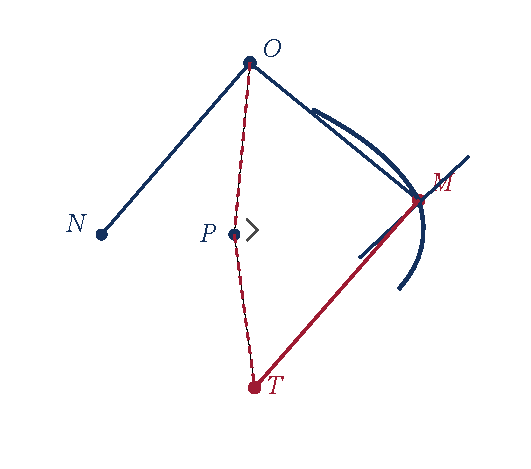
\includegraphics[width=0.45\textwidth]{figuras/pdf/cap07-fig3.pdf}
\caption{Construcción del plano polar de un rayo refractado: el punto
$O$, la paralela $ON$ a la vibración de Neumann, el punto $M$ sobre la superficie de onda, el pie de
la perpendicular $P$ y el punto $T$ tal que $OT=R^2/OP$.}
\label{fig:cap7-3}
\end{figure}

Tomemos luego sobre la prolongación de $OP$ un punto tal que
\[
OT=\frac{R^2}{OP}.
\]
Unamos $MT$; el plano llevado por $ON$ paralelamente a $MT$ se llama el
plano polar del rayo refractado considerado.

Resulta de esta definición que, si se cambia la dirección del plano de
separación haciendo variar al mismo tiempo la dirección del rayo
incidente, pero de tal manera que la del rayo refractado no cambie, el
plano polar tampoco cambiará, con tal de que el índice de refracción del
primer medio permanezca el mismo; la dirección de este plano depende, por
el contrario, del índice de refracción del primer medio.

He aquí ahora en qué consiste el teorema de Mac-Cullagh.

En el caso de la refracción uniradial, se obtendrá el desplazamiento de
un punto cualquiera del primer medio componiendo los desplazamientos
debidos a la vibración incidente y a la vibración reflejada; en cuanto al
desplazamiento de un punto del segundo medio, se reducirá al
desplazamiento debido a la sola vibración refractada que subsiste, puesto
que hemos supuesto el nicol orientado de manera que extinga la segunda
vibración refractada.

Si, pues, construimos en un punto del plano de separación tres rectas que
representen en magnitud y dirección la vibración refractada, la vibración
incidente y la vibración reflejada, la primera será la suma geométrica
de las otras dos. Estas tres rectas están, pues, en un mismo plano.

\begin{enunciado}{Teorema de Mac-Cullagh (reflexión cristalina)}
El análisis de Mac-Cullagh muestra que este plano no es otro que el plano
polar de la vibración refractada.
\end{enunciado}

\noindent\textbf{224.} Propongámonos ahora el siguiente problema:

Conociendo en magnitud y dirección la vibración incidente, construir la
vibración reflejada y las dos vibraciones refractadas.

La construcción de Huygens nos permitirá primero, conociendo el plano de
la onda incidente, construir los planos de la onda reflejada y de las dos
ondas refractadas; conoceremos igualmente el rayo reflejado y los dos
rayos refractados.

Deduciremos de ello las \emph{direcciones} de las dos vibraciones
refractadas $OR'$ y $OR''$; puesto que, en la teoría de Neumann, la
vibración refractada debe estar llevada en el plano de la onda
perpendicularmente al rayo (§215).

Construyamos luego los planos polares de las dos vibraciones refractadas;
estos planos polares cortarán el plano de la onda incidente según las
dos \emph{direcciones uniradiales}.

Sea $OI$ la vibración incidente dada, la descompondremos, por la regla
del paralelogramo, en dos componentes $OI'$ y $OI''$ dirigidas según
estas direcciones uniradiales.

El primer plano polar que pasa por $OR'$ y $OI'$ cortará la onda
reflejada según una recta $OS'$. Terminamos el paralelogramo $OI'R'S'$,
del cual un lado es $OI'$ y del cual el otro lado y la diagonal están
dirigidos según $OS'$ y $OR'$.\footnote{El original nombra estas dos
rectas en el orden «OR' et OS'»; como la vibración refractada es la suma
geométrica de la incidente y la reflejada (§223), la diagonal es $OR'$
y el otro lado $OS'$, tal como se precisa enseguida para el segundo
paralelogramo y como muestra la figura.} Entonces $OR'$ representará, no solamente
en dirección, sino en magnitud, la primera vibración refractada, y $OS'$
representará en magnitud y dirección lo que sería la vibración reflejada
si la vibración incidente se redujera a $OI'$.

\begin{figure}[h]
\centering
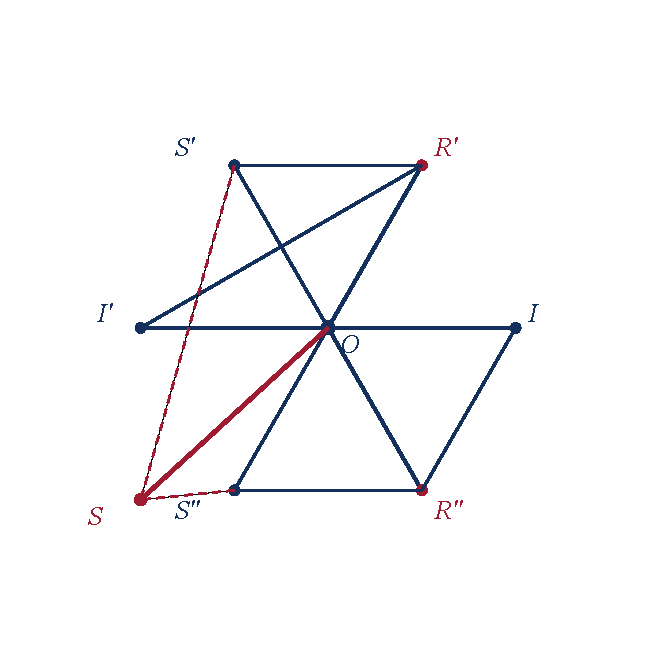
\includegraphics[width=0.6\textwidth]{figuras/pdf/cap07-fig4.pdf}
\caption{Construcción de la vibración reflejada y de las dos vibraciones
refractadas a partir de la incidente $OI$, descompuesta en $OI'$ y
$OI''$ según las direcciones uniradiales.}
\label{fig:cap7-4}
\end{figure}

Se construiría de la misma manera un segundo paralelogramo $OI''R''S''$,
del cual un lado sería $OI''$; del cual la diagonal $OR''$ representaría
en magnitud y dirección la segunda vibración refractada; del cual, en
fin, el segundo lado $OS''$ representaría lo que sería la vibración
reflejada si la vibración incidente se redujera a $OI''$.

No quedará luego más que componer $OS'$ y $OS''$ por la regla del
paralelogramo para tener la vibración reflejada total $OS$.

\subsubsection{Observación}

\noindent\textbf{225. Observación.} — Es fácil darse cuenta, por lo que
precede, de por qué los fenómenos de la reflexión cristalina se apartan
tanto más de los de la reflexión vítrea cuanto más se acerca el índice
del primer medio al índice medio del cristal. En efecto, la separación
entre los dos órdenes de fenómenos será tanto mayor cuanto más se aparte
el plano polar definido más arriba del plano $NOP$; es decir, que el
ángulo $PTM$ será más próximo a $90^{\circ}$. Siendo poco birrefringentes las
sustancias conocidas, el ángulo $POM$ es pequeño y, por consiguiente,
$PM$ es pequeño.

Para que el ángulo $PTM$ no sea pequeño, hace falta que $PT$ sea pequeño.
Ahora bien:
\[
PT=\frac{R^2}{OP}-OP.
\]
Hace falta, pues, que $OP$ sea muy cercano a $R$. Ahora bien, $OP/R$ es la
razón de la velocidad de propagación de la onda refractada a la de la
onda incidente. Estas dos velocidades deben, pues, ser muy cercanas, lo
que exige que los índices medios de los dos medios sean poco diferentes.

\subsection{Teoría de M.~Sarrau}
\label{sec:reflexion-sarrau}

\noindent\textbf{226.}\footnote{\emph{Journal de Liouville}, segunda
serie, t.~XIII.} M.~Sarrau supone:

$1^\circ$ Que la verdadera vibración tiene por componentes las
cantidades que hemos llamado más arriba X, Y y Z;

$2^\circ$ Admite además los principios fundamentales de la teoría de la
reflexión debida a Cauchy, y según los cuales las tres componentes del
desplazamiento serían continuas así como sus derivadas primeras, pero a
condición de tener en cuenta, junto a los rayos transversales
observables, rayos longitudinales evanescentes e inaccesibles a la
experiencia.

Hemos visto más arriba (§216) cuáles eran las consecuencias de los
principios admitidos por Cauchy. Si $\xi_1,\eta_1,\zeta_1$ son las tres
componentes del desplazamiento debido a la luz transversal (tomando el
plano de incidencia por plano de las $xz$ y el plano de separación por
plano de las $xy$), las cantidades
\[
\eta_1,\qquad \frac{d\zeta_1}{dy}-\frac{d\eta_1}{dz},\qquad
\frac{d\xi_1}{dz}-\frac{d\zeta_1}{dx},\qquad
\frac{d\eta_1}{dx}-\frac{d\xi_1}{dy},
\]
son funciones continuas. Si además la velocidad imaginaria de las ondas
longitudinales es la misma en todos los medios, $\xi_1$ es también una
función continua. Aunque por lo demás esta condición no se cumpla,
$\xi_1$ es todavía aproximadamente continua.

Aquí las tres componentes de la verdadera vibración son X, Y y Z; luego
X, Y y
\[
\xi=\frac{d\mathrm{Z}}{dy}-\frac{d\mathrm{Y}}{dz},\qquad
\eta=\frac{d\mathrm{X}}{dz}-\frac{d\mathrm{Z}}{dx},\qquad
\zeta=\frac{d\mathrm{Y}}{dx}-\frac{d\mathrm{X}}{dy}
\]
son funciones continuas. Estos son precisamente los resultados a los que
conducía la teoría de Neumann y Mac-Cullagh; hay, pues, concordancia
perfecta entre las dos teorías.

Importa precisar, en el caso de los medios anisótropos, lo que se debe
entender por rayo longitudinal; las vibraciones longitudinales están
dirigidas no según el rayo, sino normalmente al plano de la onda.

Añadamos que la teoría de M.~Sarrau conduciría al mismo resultado si, en
lugar de tomar por punto de partida las ideas de Cauchy, hubiera supuesto
la existencia de una capa de paso y la variación continua de los
coeficientes del polinomio que hemos llamado $W_2$.

La teoría de la doble refracción de Fresnel (§149) combinada con los
principios de la teoría de la reflexión de Cauchy conduce a resultados
incompatibles con las observaciones.

No ocurre lo mismo si se admite que la verdadera vibración es la de
Fresnel y que existe una capa de paso; los resultados a los que se llega
así no difieren de los que se pueden deducir de las otras dos teorías.

Gracias a la hipótesis de la capa de paso, los fenómenos de la reflexión
cristalina no permiten decidir entre las tres teorías de la doble
refracción; las ecuaciones del §218 conservan en efecto siempre la
misma forma cualquiera que sea la de estas tres teorías que se adopte;
solo difiere la interpretación física. Para M.~Sarrau, son X, Y, Z; para
Neumann, es $\xi,\eta,\zeta$; para Fresnel, son $u,v,w$ los que
representan las componentes de la verdadera vibración. Pero la forma
analítica de las ecuaciones y, por consiguiente, los fenómenos
observables siguen siendo los mismos en estos tres casos.

\section{Reflexión metálica}
\label{sec:reflexion-metalica}

\noindent\textbf{227. Propagación de la luz en un medio absorbente.} —
Los medios opacos, como los metales, deben considerarse, no como
absolutamente impermeables a la luz, puesto que en lámina delgada gozan
de cierta transparencia, sino como dotados de un poder absorbente
considerable.

Veamos cómo se puede concebir la propagación de la luz en un medio
semejante.

Las tres componentes del desplazamiento serán las partes reales de
funciones de la forma
\[
\xi=\mathrm{A}e^{iP},\qquad \eta=\mathrm{B}e^{iP},\qquad
\text{donde}\quad P=\frac{2\pi}{\lambda}(\alpha x+\beta y+\gamma z-Vt).
\]
Pero las cantidades A, B, C, que son proporcionales a la amplitud de la
vibración, deberán decrecer muy rápidamente a medida que el rayo se
propague. La hipótesis más natural será suponer que A, B, C son de la
forma
\[
\mathrm{A}=\mathrm{A}_0e^{-Q},\qquad \mathrm{B}=\mathrm{B}_0e^{-Q},
\qquad \mathrm{C}=\mathrm{C}_0e^{-Q},
\]
o
\[
Q=lx+my+nz;
\]
siendo $\mathrm{A}_0,\mathrm{B}_0,\mathrm{C}_0,l,m$ y $n$ constantes.

Se ve así que, en la propagación de una onda plana en un medio
absorbente, hay que considerar dos planos que desempeñan ambos un papel
importante: el plano de la onda
\[
\alpha x+\beta y+\gamma z=0
\]
y el plano de absorción
\[
lx+my+nz=0.
\]
Las expresiones de $\xi,\eta$ y $\zeta$ pueden también
escribirse\footnote{Con $\mathrm{A}=\mathrm{A}_0e^{-Q}$ se tiene, en
rigor, $\mathrm{A}e^{iP}=\mathrm{A}_0e^{i(P+iQ)}$, es decir, coeficientes
$\frac{2\pi}{\lambda}\alpha+il$, etc., y no $\frac{2\pi}{\lambda}\alpha-il$;
con ese signo la parte imaginaria de $1/V'^2$ resultaría igual a
$+\frac{\lambda}{\pi V^2}(\alpha l+\beta m+\gamma n)$, positiva. Poincaré
adopta en todo lo que sigue (§§227--230) la convención de signo opuesta
para la parte imaginaria ---equivalente a reemplazar las cantidades
imaginarias por sus conjugadas---, de la que dependen la forma
$m(\cos\chi-i\sin\chi)$ del índice y la ecuación (1) del §228. Como el
cambio es global, no altera ninguna conclusión física, y se conserva aquí
el texto del original.}
\[
\xi=\mathrm{A}_0e^{iP'},\qquad \eta=\mathrm{B}_0e^{iP'},\qquad
\zeta=\mathrm{C}_0e^{iP'},
\]
poniendo
\[
P'=\left[\left(\frac{2\pi}{\lambda}\alpha-il\right)x
+\left(\frac{2\pi}{\lambda}\beta-im\right)y
+\left(\frac{2\pi}{\lambda}\gamma-in\right)z-\frac{2\pi V t}{\lambda}\right].
\]
Dicho de otro modo, todo pasa como si el plano de la onda tuviera por
ecuación
\[
P''=\left(\frac{2\pi}{\lambda}\alpha-il\right)x
+\left(\frac{2\pi}{\lambda}\beta-im\right)y
+\left(\frac{2\pi}{\lambda}\gamma-in\right)z=0
\]
y si la velocidad de propagación tuviera por expresión
\[
V'=\dfrac{V}{\sqrt{\left(\alpha-\dfrac{il\lambda}{2\pi}\right)^2
+\left(\beta-\dfrac{im\lambda}{2\pi}\right)^2
+\left(\gamma-\dfrac{in\lambda}{2\pi}\right)^2}}.
\]
Llamaremos al plano $P''=0$ plano imaginario de la onda, y a la velocidad
$V'$, velocidad imaginaria de la onda.

Para que el rayo vaya constantemente debilitándose a medida que se
propaga, es necesario y suficiente que la normal al plano de la onda
llevada en el sentido de la propagación del rayo y la normal al plano de
absorción llevada en el sentido de la extinción formen un ángulo agudo.
Esta condición se escribe:
\[
\alpha l+\beta m+\gamma n>0.
\]
Ahora bien, la parte imaginaria de $1/V'^2$ es igual a
\[
-\frac{\lambda}{\pi V^2}(\alpha l+\beta m+\gamma n).
\]
Esta parte imaginaria\footnote{El original dice «Cette partie réelle»,
errata evidente: la frase anterior acaba de calcular la parte
\emph{imaginaria} de $1/V'^2$, y el párrafo siguiente vuelve a hablar de
«la partie imaginaire du carré de $1/V'$».} debe, pues,
ser negativa.

En resumen, un medio absorbente se comporta como si su índice de
refracción fuera imaginario. Sea
\[
m(\cos\chi-i\sin\chi)
\]
este índice. Como el índice de refracción es proporcional al inverso de
la velocidad, es decir, aquí a $1/V'$, y que la parte imaginaria del
cuadrado de $1/V'$ debe ser negativa, el ángulo $\chi$ deberá estar
comprendido entre $0$ y $\pi/2$.

\noindent\textbf{228.} Dicho esto, propongámonos el siguiente problema:

Un rayo luminoso cae sobre una superficie metálica con una incidencia
igual a $\varphi$; ¿cuál es la dirección del plano imaginario de la
onda, del plano de la onda, del plano de absorción, y el coeficiente de
absorción?

El plano de absorción no puede ser más que el plano de separación de los
dos medios, que tomamos por plano de las $xy$. Tomaremos el plano de
incidencia por plano de las $xz$.

Sea $r'$ el ángulo del plano imaginario de la onda con el plano de las
$xy$, es decir, el ángulo imaginario de refracción. Sea $r$ el ángulo
real de la onda con el plano de las $xy$, es decir, el ángulo real de
refracción.

El plano imaginario de la onda deberá tener por ecuación
\[
x\sin r'+z\cos r'=0,
\]
o\footnote{A partir de aquí Poincaré reinicia la numeración de las
ecuaciones dentro de la sección sobre la reflexión metálica.}
\setcounter{equation}{0}
\begin{equation}
\sin r'=\frac{\sin\varphi}{m}(\cos\chi+i\sin\chi),
\end{equation}
Se tendrá por otra parte
\[
P=\frac{2\pi}{\lambda}(x\sin r+z\cos r-Vt),
\]
y
\[
Q=\varkappa z,
\]
siendo $\varkappa$ el coeficiente de absorción.

La ecuación del plano imaginario de la onda se escribirá entonces
\[
x\frac{2\pi}{\lambda}\sin r+z\left(\frac{2\pi}{\lambda}\cos r-i\varkappa\right)=0,
\]
Se tiene, pues:
\[
\tan r'=\dfrac{\dfrac{2\pi}{\lambda}\sin r}{\dfrac{2\pi}{\lambda}\cos r-i\varkappa}.
\]
De la ecuación (1) se saca fácilmente $\cot r'$ bajo la forma:
\[
\cot r'=\mathrm{A}-i\mathrm{B};
\]
se tiene entonces
\[
\cot r=\mathrm{A},\qquad \varkappa=\frac{2\pi\mathrm{B}\sin r}{\lambda};
\]
lo que determina el ángulo real de refracción y el coeficiente de
absorción.

\subsection{Teoría de Cauchy}
\label{sec:reflexion-metalica-cauchy}

\noindent\textbf{229. Ecuaciones del movimiento luminoso en un medio
absorbente.} — Se han propuesto diversas formas para las ecuaciones del
movimiento en un medio absorbente. Una de las más generales es la de
Voigt,\footnote{\emph{Göttinger Nachrichten}, 1884, p.~137 y ss.} que se
escribe:
\begin{equation}
\rho\frac{d^2\xi}{dt^2}=\Delta\xi+a\xi+b\frac{d\xi}{dt}+c\frac{d\Delta\xi}{dt}
+e\frac{d^2\Delta\xi}{dt^2},
\end{equation}
con otras dos ecuaciones análogas para $\eta$ y $\zeta$, a las cuales hay
que añadir la condición de transversalidad $\Theta=0$.

La teoría electromagnética de la luz ha conducido a Maxwell a una
ecuación de la misma forma, pero donde los coeficientes $a,c$ y $e$ son
nulos.

Estas ecuaciones, u otras análogas, no pueden evidentemente dar cuenta de
la propagación de la luz en los medios poco absorbentes, que producen un
espectro de rayas o de bandas. Cualquiera que sea el número de derivadas
parciales de $\xi$ que en ellas se introduzca, nunca se llegará a dar
cuenta de la prodigiosa variedad de estos espectros. En cambio, estas
ecuaciones parecen dar cuenta bastante bien de los fenómenos ópticos que
presentan los metales.

Busquemos satisfacer la ecuación (2) haciendo
\[
\xi=\mathrm{A}e^{\frac{2i\pi}{V'\tau}(\alpha'x+\beta'y+\gamma'z-V't)}.
\]
La parte real de esta exponencial imaginaria será entonces el verdadero
valor de $\xi$; $\tau$ será el período de la vibración, $V'$ será la
velocidad imaginaria de propagación; $\alpha',\beta',\gamma'$ serán los
cosenos directores del plano imaginario de la onda, de tal manera que se
tendrá
\begin{equation}
\alpha'^2+\beta'^2+\gamma'^2=1.
\end{equation}
Se encuentra entonces, sustituyendo este valor de $\xi$ en (2),
suprimiendo los factores comunes y teniendo en cuenta
(3):\footnote{El original imprime $\dfrac{4\pi^2e}{\tau}$ en el último
término; como $e$ multiplica a una segunda derivada respecto del tiempo,
debe leerse $\dfrac{4\pi^2e}{\tau^2}$. En cuanto a los dos términos
imaginarios, la sustitución directa con el exponente
$\dfrac{2i\pi}{V'\tau}(\ldots-V't)$ los da con signo $-$; el cambio
simultáneo de ambos signos corresponde a la misma convención señalada en
el §227 y no afecta a la conclusión que sigue.}
\begin{equation}
V'^2\left(a+\frac{2i\pi b}{\tau}+\frac{4\pi^2\rho}{\tau^2}\right)
=\frac{4\pi^2}{\tau^2}\left(1+\frac{2i\pi c}{\tau}-\frac{4\pi^2 e}{\tau^2}\right).
\end{equation}
Esta ecuación muestra que la velocidad imaginaria $V'$ depende de $\tau$
y, por consiguiente, de la longitud de onda, pero no depende de la
dirección del plano de la onda.

Por consiguiente, el índice imaginario de refracción $\sin r'/\sin\varphi$
es una constante que depende del color, pero es independiente de la
incidencia. No ocurriría lo mismo con el índice real de refracción
$\sin r/\sin\varphi$.

\noindent\textbf{230. Teoría de Cauchy.}\footnote{\emph{Nouveaux exercices
de mathématiques}, \emph{Journal de Liouville}, primera serie, t.~VII,
p.~338.} — Cauchy supone que las hipótesis que sirven de base a su teoría
de la reflexión vítrea siguen siendo aplicables a la reflexión metálica.

De estas hipótesis resulta, como lo hemos visto, que si el plano de
separación se toma como plano de las $xy$, las funciones
\[
\xi,\qquad \eta,\qquad \frac{d\zeta}{dy}-\frac{d\eta}{dz},\qquad
\frac{d\xi}{dz}-\frac{d\zeta}{dx},\qquad \frac{d\eta}{dx}-\frac{d\xi}{dy}
\]
son continuas.

Acabamos de ver que, en un medio metálico, las ecuaciones del movimiento
son las mismas que si el índice de refracción fuera imaginario. Por otra
parte, en las ideas de Cauchy, las condiciones en el límite son las
mismas que en el caso de la reflexión vítrea. Es, pues, inútil volver a
empezar los cálculos; las fórmulas de la reflexión vítrea deben seguir
siendo aplicables; basta con reemplazar en ellas el índice de refracción
por su valor imaginario.

Sabemos que, en el estudio de la reflexión vítrea, la teoría de Cauchy y
la de Fresnel conducen a los mismos resultados. Fresnel demuestra que la
razón de la vibración reflejada a la vibración incidente es igual a
\[
\frac{\sin(r-\varphi)}{\sin(r+\varphi)}
\]
si la luz está polarizada en el plano de incidencia, y a
\[
\frac{\tan(\varphi-r)}{\tan(\varphi+r)}
\]
si la luz está polarizada perpendicularmente a este plano.

Los ángulos $\varphi$ y $r$ son los ángulos de incidencia y de
refracción. Si se llama N al índice de refracción, estas dos razones son
iguales respectivamente a
\[
\mathrm{A}=\frac{\cos\varphi-\sqrt{\mathrm{N}^2-\sin^2\varphi}}
{\cos\varphi+\sqrt{\mathrm{N}^2-\sin^2\varphi}}
\qquad\text{y}\qquad
\mathrm{A}'=\frac{\mathrm{N}^2\cos\varphi-\sqrt{\mathrm{N}^2-\sin^2\varphi}}
{\mathrm{N}^2\cos\varphi+\sqrt{\mathrm{N}^2-\sin^2\varphi}}.
\]
Estas fórmulas se deducirían sin dificultad de las que hemos dado más
arriba (§203).

Si $\alpha,\beta,\gamma$ son los cosenos directores de la onda reflejada,
$\lambda$ la longitud de onda y V la velocidad de propagación en el
primer medio, el desplazamiento debido a la vibración reflejada será la
parte real de
\[
\mathrm{A}e^{iP}\qquad\text{o}\qquad \mathrm{A}'e^{iP},
\]
o\footnote{El original imprime $\mathrm{P}=\dfrac{2i\pi}{\lambda}(\ldots)$;
el factor $i$ sobra, pues ya figura en el exponente $i\mathrm{P}$ y
$\mathrm{P}$ debe ser real para que el desplazamiento reflejado sea
$\mathrm{A}_0\cos(\mathrm{P}+\psi)$.}
\[
\mathrm{P}=\frac{2\pi}{\lambda}(\alpha x+\beta y+\gamma z-Vt).
\]
Si se pasa a la reflexión metálica, hace falta dar a N un valor
imaginario; A y A' son entonces imaginarios y se tiene
\[
\mathrm{A}=\mathrm{A}_0e^{i\psi},\qquad \mathrm{A}'=\mathrm{A}_0'e^{i\psi'}.
\]
Entonces el desplazamiento debido a la luz reflejada será
\[
\mathrm{A}_0\cos(\mathrm{P}+\psi)
\]
si el plano de polarización es el plano de incidencia, y
\[
\mathrm{A}_0'\cos(\mathrm{P}+\psi')
\]
si el plano de polarización es normal al plano de incidencia.

Habrá, pues, polarización elíptica, y la diferencia de fase de las dos
componentes del rayo reflejado será $\psi-\psi'$.

La experiencia confirma muy suficientemente las fórmulas de Cauchy.

% ============================================================
% Fin del Capítulo VII.
% ============================================================


% ============================================================
% Capítulo VIII — Aberración astronómica
% Traducción de "Théorie mathématique de la lumière" (1889), cap. VIII
% Original: §§231-243, páginas impresas 379-401
% Último capítulo del Volumen I; termina con las Conclusiones del volumen.
% ============================================================
\chapter{Aberración astronómica}
\label{cap:aberracion}

\noindent\textbf{231.} En el estudio de los diversos fenómenos ópticos que
hemos considerado hasta aquí, siempre hemos supuesto que el movimiento
vibratorio que da origen a la luz tenía lugar en un fluido particular, el
éter, repartido tanto en los medios materiales transparentes como en los
espacios interplanetarios. Es evidentemente imposible concebir la
propagación de la luz del Sol a la Tierra sin la existencia de un medio
elástico; en cambio, puede parecer superfluo y quizás poco filosófico
suponer la existencia del éter en los medios materiales. Sin embargo, el
fenómeno de la aberración astronómica, que pone en evidencia el movimiento
relativo del éter y del medio ponderable que este penetra, parece oponerse
absolutamente a la supresión de esta hipótesis; o, al menos, si se
rechazara esta hipótesis, la explicación de la aberración astronómica
tropezaría con dificultades tales que es preferible mantenerla. Digamos,
pues, algunas palabras sobre este fenómeno.

Se sabe que, cuando se apunta a un astro con un anteojo, el astro no se
encuentra sobre la recta que une el centro óptico del objetivo con el
punto de cruce de los hilos del retículo, es decir, sobre el eje óptico del
instrumento. No vemos, pues, un astro en su dirección real, y el ángulo de
esta dirección con el del eje óptico del anteojo se llama la \emph{aberración};
este desvío angular puede llegar hasta $20''$.

\section{Explicación de Bradley}

\noindent\textbf{232. Explicación de Bradley.} — La primera explicación
del fenómeno de la aberración se debe a Bradley; se apoya, por lo demás, en
la teoría de la emisión, que era entonces la adoptada. Sea $OA$
(figura~\ref{fig:cap8-1}) una recta que representa, en magnitud y
dirección, la velocidad de la que están animados los corpúsculos luminosos
emitidos por el astro. El observador, situado en la superficie de la
Tierra y arrastrado por el movimiento de esta, no podrá comprobar más que
la velocidad relativa del corpúsculo.

\begin{figure}[h]
\centering
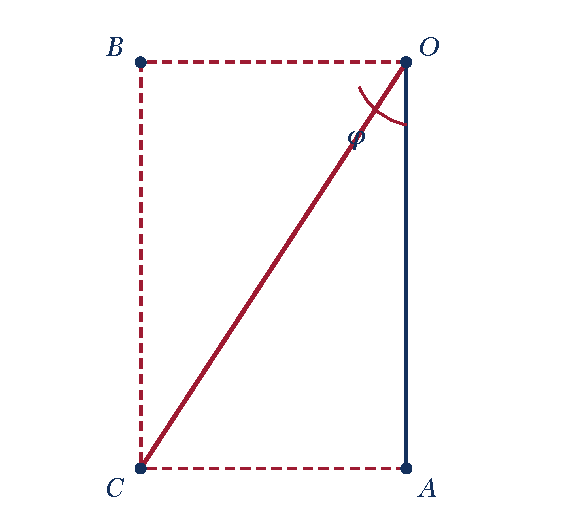
\includegraphics[width=0.7\textwidth]{figuras/pdf/cap08-fig1.pdf}
\caption{Composición de velocidades en la explicación de Bradley: $OA$
es la velocidad real de la luz, $OB$ la velocidad de arrastre del
observador (invertida), y $OC$ la diagonal que da la dirección
aparente.}
\label{fig:cap8-1}
\end{figure}

Esta velocidad relativa se obtendrá componiendo la velocidad real $OA$ con
la velocidad $OB$, igual y de signo contrario a la velocidad de arrastre
del observador; será, pues, $OC$. El observador verá el astro según la
dirección $CO$ en lugar de verlo en la dirección $AO$; por consiguiente, la
aberración será el ángulo $\varphi$. El valor de este ángulo será
evidentemente máximo cuando el cuadrilátero $OABC$ se vuelva rectángulo. En
este caso tendremos
\[
\tan\varphi = \frac{OB}{OA};
\]
o bien, siendo la velocidad $OA$ de la luz de unos $300\,000$ kilómetros
por segundo, y la velocidad de arrastre de un punto de la superficie de la
Tierra de solo $30$ kilómetros, tendremos aproximadamente
\[
\tan\varphi = \frac{30}{300\,000} = \frac{1}{10\,000}.
\]
El ángulo $\varphi$ correspondiente a este valor de la tangente es, como ya
hemos dicho, de unos $20$ segundos.

\begin{notahistorica}
James Bradley descubrió la aberración de la luz estelar en el curso de
observaciones realizadas entre 1725 y 1728, mientras intentaba medir la
paralaje de las estrellas, y comunicó su explicación a la Royal Society a
comienzos de 1729 (enero de 1728 según el calendario inglés de la época).
Fue la primera prueba observacional directa del movimiento de la Tierra
en el espacio —independiente de la paralaje, que no se mediría con éxito
hasta más de un siglo después— y permitió, de paso, una de las primeras
estimaciones precisas de la velocidad de la luz.
\end{notahistorica}

\section{Explicación ondulatoria}

\noindent\textbf{233. Explicación elemental en la teoría de las
ondulaciones.} — En la hipótesis de las ondulaciones, la explicación
elemental del fenómeno es igualmente simple. Sea $A$
(figura~\ref{fig:cap8-2}) el centro óptico del objetivo de un anteojo, $B$
el cruce de los hilos del retículo, y $AE$ la dirección de un rayo luminoso
proveniente de una estrella $E$. Si la Tierra estuviera inmóvil, los tres
puntos $E$, $A$ y $B$ estarían en línea recta; pero, a causa del movimiento
de la Tierra, el punto $B$ ha pasado a $B'$ durante el tiempo que el rayo
luminoso empleó en recorrer el camino $AB'$. El rayo luminoso que viene a
herir el ojo del observador tiene, pues, por dirección real $EAB'$,
mientras que su dirección aparente es la del eje óptico, es decir, la de
una paralela a $BA$ trazada por $B'$; la aberración es, por tanto, el
ángulo $BAB' = \varphi$. Si designamos por $V$ la velocidad de propagación
de las ondas luminosas en el éter inmóvil y por $v$ la velocidad de un
punto de la superficie de la Tierra, supuesta paralela a $BB'$, tendremos:
\[
\sin\varphi = \frac{BB'}{AB'} = \frac{vt}{Vt} = \frac{v}{V}.
\]

\begin{figure}[h]
\centering
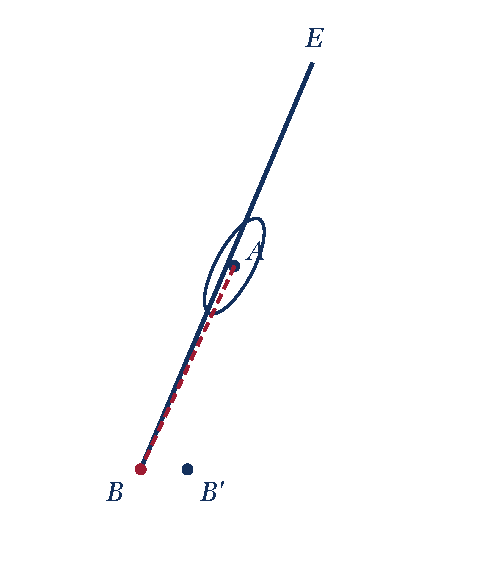
\includegraphics[width=0.55\textwidth]{figuras/pdf/cap08-fig2.pdf}
\caption{Explicación ondulatoria de la aberración: el rayo real $EAB'$
y la dirección aparente, paralela a $AB$ trazada por $B'$.}
\label{fig:cap8-2}
\end{figure}

Como el ángulo $\varphi$ es muy pequeño, se puede confundir el valor del
ángulo con el de su tangente o con el de su seno; por consiguiente,
volvemos a encontrar para el máximo de $\varphi$ el mismo valor que por la
explicación de Bradley.

Este razonamiento supone que el éter contenido en el anteojo está inmóvil
en el espacio, que no participa del movimiento de la Tierra. En efecto,
cuando un medio elástico se desplaza, las vibraciones que transmite
participan de ese movimiento; así, se sabe que la velocidad del sonido en
el aire en movimiento depende de la velocidad del aire, y la influencia del
viento sobre la velocidad de propagación del sonido es una prueba
evidente. Por consiguiente, si el éter contenido en el anteojo se
encontrara arrastrado con ella, la velocidad de propagación de la luz en el
tubo del anteojo sería la compuesta $V'$ de la velocidad $V$ y de la
velocidad de arrastre $v$ del medio elástico. Pero, por otra parte,
participando el observador del movimiento de la Tierra, la velocidad
relativa de la luz sería para él la resultante de $V'$ y de $-v$, es decir,
$V$. Los fenómenos observados serían entonces los mismos que si el éter y
el observador estuvieran inmóviles; por consiguiente, no habría
aberración, consecuencia contraria a la experiencia.

\section{El arrastre parcial del éter}

\noindent\textbf{234. El éter contenido en un medio material en movimiento
es parcialmente arrastrado.} — Pero, ¿está el éter inmóvil cuando atraviesa
un medio más refringente que el aire? Una experiencia de los astrónomos de
Greenwich nos permite responder que el éter es \emph{parcialmente} arrastrado
y que su velocidad de arrastre depende del índice de refracción de la
sustancia atravesada por la luz. En el aire mismo debería haber un arrastre
parcial del éter, muy débil es cierto puesto que el aire es poco
refringente; pero para que la explicación precedente fuera del todo
rigurosa, habríamos debido suponer que el tubo del anteojo estaba vacío de
aire.

La experiencia de los astrónomos de Greenwich consistía en apuntar una
estrella con un anteojo lleno de aire, y luego con el mismo anteojo cuyo
tubo estaba lleno de agua; comprobaron que, en ambos casos, la posición
aparente del astro era la misma. Analicemos esta experiencia y busquemos
sus consecuencias.

\begin{figure}[h]
\centering
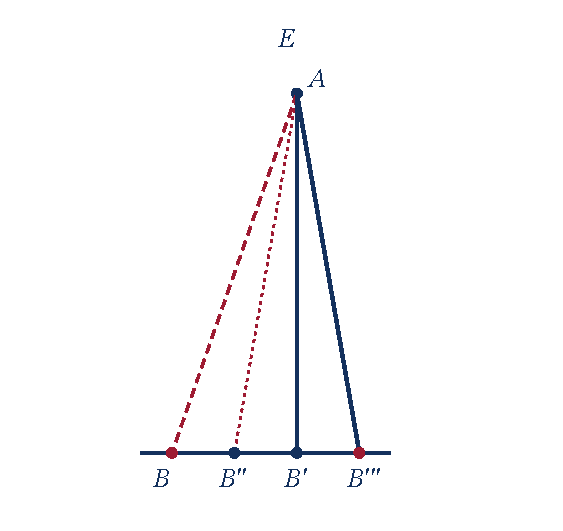
\includegraphics[width=0.7\textwidth]{figuras/pdf/cap08-fig3.pdf}
\caption{El experimento de los astrónomos de Greenwich: posiciones del
cruce de los hilos del retículo bajo las distintas hipótesis sobre el
arrastre del éter en el agua.}
\label{fig:cap8-3}
\end{figure}

Sea $EAB'$ (figura~\ref{fig:cap8-3}) la dirección de propagación de la luz
en el anteojo, que supondremos vacío de aire, en la hipótesis en que el
éter no participa del movimiento de la Tierra. Si admitimos que ocurre lo
mismo para el éter contenido en el agua en movimiento, el rayo $EC$,
penetrando oblicuamente en ese medio, se refractaría siguiendo $AB''$
acercándose a la normal. La imagen de la estrella se formaría en $B''$.
Ahora bien, propagándose la luz más lentamente en el agua que en el vacío,
el punto de cruce $B$ de los hilos del retículo del anteojo se encontrará,
a causa del movimiento de la Tierra, en un punto $B'''$, situado a la
derecha de $B'$, cuando las vibraciones luminosas lleguen al plano del
retículo. Estando los puntos $B''$ y $B'''$, el primero a la izquierda, el
segundo a la derecha de $B'$, no pueden coincidir, y por consiguiente la
imagen de la estrella ya no se encontraría en el punto de cruce de los
hilos del retículo. Debemos, pues, admitir, para estar de acuerdo con la
experiencia, que el éter que propaga la luz en el agua es arrastrado, al
menos parcialmente, por el movimiento de la Tierra.

Busquemos la velocidad de arrastre. Designando por $i$ y $r$ los ángulos de
incidencia y de refracción de la luz cuando penetra en el anteojo lleno de
agua, tendremos
\[
\frac{\sin i}{\sin r} = n.
\]
Por lo demás, siendo los ángulos $i$ y $r$ muy pequeños, los senos pueden
confundirse con las tangentes, y la relación precedente se convertirá en
\[
n = \frac{\tan i}{\tan r} = \frac{\tan BAB'}{\tan BAB''} = \frac{BB'}{BB''}.
\]
De ahí sacamos
\begin{equation}
BB'' = \frac{1}{n}BB'.
\end{equation}
Por otra parte, llamando $V'$ a la velocidad de propagación de la luz en el
agua y $v$ a la velocidad de arrastre del anteojo, tenemos, escribiendo que
la luz llega a $B'''$ cuando $B$ llega a ese mismo punto,
\[
AB''' = V't', \qquad BB''' = vt';
\]
de donde sacamos
\[
\frac{AB'''}{BB'''} = \frac{V'}{v}.
\]
Encontraremos de la misma manera
\[
\frac{AB'}{BB'} = \frac{V}{v}.
\]
Si confundimos las longitudes $AB'$ y $AB'''$, que difieren muy poco,
obtendremos, dividiendo una por la otra, las dos relaciones precedentes,
\[
BB''' = \frac{V}{V'}BB',
\]
o bien, puesto que el índice de refracción es igual al cociente de las
velocidades,\footnote{La edición original imprime aquí, en la
ecuación~(2), $BB'' = n\,BB'$, con dos acentos en lugar de tres; la línea
anterior y el uso que se hace enseguida de esta relación muestran que debe
leerse $BB'''$. Esta errata no figura en la fe de erratas del volumen.}
\begin{equation}
BB''' = n\,BB'.
\end{equation}
Para que el movimiento vibratorio del éter arrastrado en el agua llegue a
$B'''$ al mismo tiempo que el punto de cruce de los hilos del retículo, es
necesario que el movimiento de arrastre del éter sea tal que el punto
$B''$ haya recorrido $B''B'''$ durante el tiempo $t'$ empleado por la luz
para ir de $A$ a $B'''$. Las relaciones (1) y (2) nos dan para el valor de
$B''B'''$
\[
B''B''' = BB''' - BB'' = \Bigl(n-\frac{1}{n}\Bigr)BB' =
\Bigl(1-\frac{1}{n^2}\Bigr)BB''';
\]
pero, puesto que $BB'''=vt'$, tendremos
\[
B''B''' = \Bigl(1-\frac{1}{n^2}\Bigr)vt'.
\]
La velocidad de arrastre del éter tendrá, pues, por valor
\[
\Bigl(1-\frac{1}{n^2}\Bigr)v.
\]

\noindent\textbf{235.} Fizeau emprendió experiencias con el objeto de
verificar el arrastre del éter por un medio material en movimiento. En
estas experiencias, dos rayos luminosos provenientes de la misma fuente
atraviesan dos tubos paralelos llenos de agua y de una longitud de $1{,}50$
metros aproximadamente; a su salida, estos rayos dan franjas de
interferencia que se observan con un ocular provisto de un micrómetro. Al
hacer que el agua de los tubos se mueva en sentido opuesto, se comprobaba
un desplazamiento de las franjas. Ese desplazamiento era, para una
velocidad de $7$ metros por segundo del agua de los tubos, de $2{,}4$
divisiones del micrómetro, es decir, casi media franja, ocupando una franja
entera $5$ divisiones del micrómetro. El cálculo efectuado en la hipótesis de que la velocidad de
arrastre del éter está dada por la expresión precedente
$\bigl(1-\tfrac{1}{n^2}\bigr)v$ conduce a un valor del desplazamiento muy
próximo al hallado experimentalmente. Además, el desplazamiento tenía lugar
tanto a la derecha como a la izquierda según el sentido del movimiento del
agua.

El desplazamiento de las franjas se debía efectivamente a este movimiento,
pues, haciendo, por medio de espejos, atravesar sucesivamente los dos tubos
a los dos rayos luminosos antes de hacerlos interferir, se evitaban las
diferencias de marcha que habrían podido resultar de variaciones desiguales
de la temperatura o de la presión en los tubos.

Las mismas experiencias, intentadas reemplazando el agua por aire, no
dieron ningún resultado; el cálculo conduce también a un desplazamiento
inapreciable de las franjas incluso para valores considerables de la
velocidad del aire.

Muy recientemente, dos físicos norteamericanos, los señores Michelson y
Morley, retomaron las experiencias de Fizeau con un aparato de mayores
dimensiones.\footnote{\emph{American Journal of Science}, vol.~XXXI, mayo
de 1886.} El agua circulaba en tubos de $6$ metros de longitud bajo una
presión de $23$ metros de altura de agua. El desplazamiento de la franja
central alcanzó casi una franja entera ($0^{\text{f}}{,}899$). Con el aire
animado de una velocidad de $25$ metros por segundo, el desplazamiento de
las franjas fue sensiblemente nulo. Las experiencias de Fizeau se
encuentran, pues, plenamente confirmadas.

\section{Velocidad de la luz en un medio en movimiento}

\noindent\textbf{236. Velocidad de la luz en un medio en movimiento.} —
Tenemos dos velocidades que considerar, por una parte la velocidad de la
luz respecto de ejes fijos en el espacio, por otra la velocidad respecto de
ejes móviles invariablemente ligados al medio en movimiento.

Para tener la velocidad respecto de los ejes fijos, debemos componer la
velocidad absoluta $V'$ con la velocidad de arrastre
$\bigl(1-\tfrac{1}{n^2}\bigr)v$ del éter. Si $\varphi$ es el ángulo de
estas dos velocidades, representadas por $AB$ y $BC$
(figura~\ref{fig:cap8-4}), la velocidad buscada será
\[
AC = V'\cos A + \Bigl(1-\frac{1}{n^2}\Bigr)v\cos C.
\]

\begin{figure}[h]
\centering
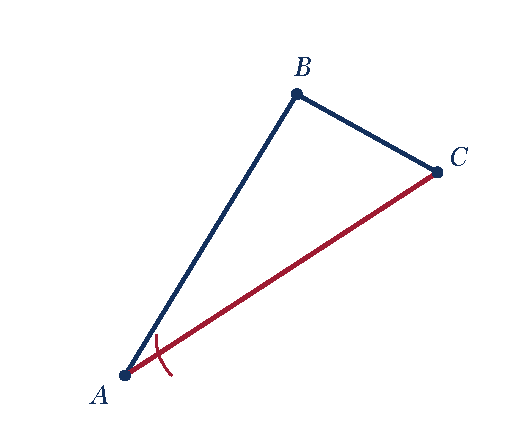
\includegraphics[width=0.75\textwidth]{figuras/pdf/cap08-fig4.pdf}
\caption{Composición de la velocidad absoluta $V'$ (dirección $AB$) y de
la velocidad de arrastre del éter (dirección $BC$): la resultante es
$AC$.}
\label{fig:cap8-4}
\end{figure}

Siendo el ángulo $A$ muy pequeño, podemos confundir su coseno con la
unidad. Despreciamos así las cantidades del orden del cuadrado de la
aberración; ahora bien, tenemos derecho a ello, pues la aberración, siendo
a lo sumo igual a $20''$ o $\tfrac{1}{10\,000}$, su cuadrado es la
$\tfrac{1}{10\,000}$-ésima parte de $20''$, es decir, $\tfrac{1}{500}$ de
segundo. Tendremos entonces
\[
AC = V' + v\Bigl(1-\frac{1}{n^2}\Bigr)\cos\varphi.
\]

Tomemos ahora ejes ligados al medio móvil. Habrá que reemplazar en la
expresión precedente la velocidad absoluta de arrastre
$v\bigl(1-\tfrac{1}{n^2}\bigr)$ por la velocidad relativa
\[
v\Bigl(1-\frac{1}{n^2}\Bigr) - v = -\frac{v}{n^2} = -v'.
\]
Por consiguiente tendremos para la velocidad de la luz respecto de estos
ejes
\[
V' - v'\cos\varphi.
\]

\section{El tiempo de recorrido en un medio en movimiento}

\noindent\textbf{237. Tiempo empleado por la luz para pasar de un punto a
otro de un medio en movimiento.} — Consideremos un rayo luminoso que va de
un punto $A_0$ a un punto $A_n$ de un medio en movimiento siguiendo la
línea quebrada $A_0A_1\ldots A_n$ (figura~\ref{fig:cap8-5}). Para pasar del
punto $A_1$ al punto $A_2$, el rayo empleará un tiempo igual a
$\dfrac{A_1A_2}{V'-v'\cos\varphi}$. Desarrollemos esta cantidad según las
potencias crecientes de $v'$, deteniéndonos en la primera potencia;
tendremos
\[
\frac{A_1A_2}{V'} + \frac{A_1A_2\cos\varphi}{V'^2}v'.
\]

\begin{figure}[h]
\centering
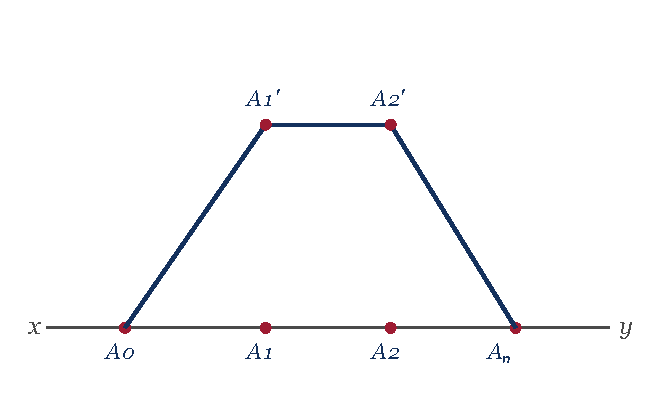
\includegraphics[width=0.85\textwidth]{figuras/pdf/cap08-fig5.pdf}
\caption{Camino en línea quebrada $A_0A_1\ldots A_n$ seguido por la luz
en un medio en movimiento.}
\label{fig:cap8-5}
\end{figure}

Si trazamos una recta $xy$ paralela a la velocidad del medio en movimiento,
el ángulo de las diversas porciones de la línea quebrada con esta recta es
precisamente el ángulo de aberración $\varphi$ que entra en la expresión
precedente; por consiguiente, $A_1A_2\cos\varphi$ es igual a la proyección
$A_1'A_2'$ de $A_1A_2$ sobre $xy$, y el tiempo empleado por la luz para ir
de $A_1$ a $A_2$ se convierte en
\[
\frac{A_1A_2}{V'} + \frac{A_1'A_2'}{V'^2}v'.
\]
Tenemos, además, $v'=\dfrac{v}{n^2}$ y $V'=\dfrac{V}{n}$, siendo $v$ la
velocidad de traslación del medio y $V$ la velocidad de la luz en el
vacío; reemplazando $v'$ y $V'$ por estos valores en la suma precedente,
tendremos
\[
\frac{A_1A_2}{V'} + A_1'A_2'\,\frac{v}{V^2}.
\]
El tiempo empleado para ir del punto $A_0$ al punto $A_n$ será la suma de
cantidades semejantes, es decir,
\[
\sum\frac{A_1A_2}{V'} + \frac{v}{V^2}A_0'A_n'.
\]
El primer término $\sum\dfrac{A_1A_2}{V'}$ representa el tiempo que
emplearía la luz si el medio estuviera en reposo; el segundo no depende más
que de la posición de los puntos extremos y de ningún modo del camino
recorrido por la luz para ir de uno al otro de esos puntos.

\section{Fenómenos ópticos en un medio en movimiento}

\noindent\textbf{238. Fenómenos ópticos en un medio en movimiento.} — Una
consecuencia importante de la fórmula precedente es que las leyes de la
reflexión y de la refracción, los fenómenos de interferencias no son
afectados por el movimiento de la Tierra.

Consideremos en particular el fenómeno de la refracción. Si $A$ y $B$
(figura~\ref{fig:cap8-6}) son dos puntos situados en dos medios diferentes,
el camino $ACB$ seguido por la luz para ir de $A$ a $B$ es tal que el
tiempo empleado para recorrer ese camino es mínimo. Para mostrar que las
leyes de la refracción son las mismas cuando los dos medios están en reposo
o en movimiento, nos basta mostrar que, si $ACB$ es el camino más corto
cuando los medios están en reposo, lo es todavía cuando los dos medios
están animados del mismo movimiento.

\begin{figure}[h]
\centering
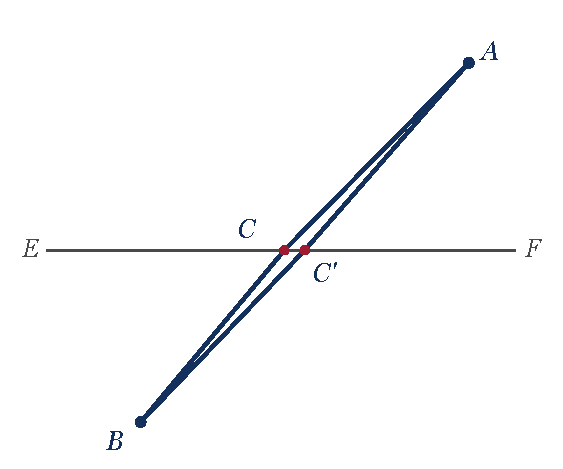
\includegraphics[width=0.6\textwidth]{figuras/pdf/cap08-fig6.pdf}
\caption{El camino mínimo $ACB$ entre dos puntos de medios distintos: su
posición no cambia cuando ambos medios se mueven con la misma
velocidad.}
\label{fig:cap8-6}
\end{figure}

Sean $T$ el tiempo empleado por la luz para ir de $A$ a $B$ por el camino
mínimo cuando los medios están en reposo; $T'$ el tiempo necesario para
recorrer un camino infinitamente vecino $AC'B$. Si $ACB$ es el que
corresponde a las leyes de la refracción, se tiene $T<T'$. Ahora bien,
según lo que acabamos de decir anteriormente, los tiempos empleados para
recorrer los caminos $ACB$ y $AC'B$ en el caso en que los medios están
animados de un movimiento de traslación cuya velocidad es $v$, son
\[
T_1 = T + \frac{v}{V^2}A'B', \qquad T_1' = T' + \frac{v}{V^2}A'B',
\]
siendo $A'B'$ la proyección de $AB$ sobre una recta paralela a la velocidad
$v$; no difieren de $T$ y de $T'$ más que por una misma cantidad. Si,
pues, se tiene $T<T'$, tendremos $T_1<T_1'$, y el camino más corto en los
medios en reposo seguirá siendo el más corto cuando los medios estén en
movimiento. Las leyes de la refracción son, por consiguiente, las mismas
en los dos casos.

Los fenómenos de interferencia de los rayos luminosos tampoco dependen del
movimiento del medio donde se producen. Si $T$ y $T'$ son los tiempos
empleados por dos rayos para ir de un punto $A_0$ a un punto $A_n$ en el
caso en que el medio está en reposo, estos tiempos serán ambos aumentados
en la misma cantidad si se supone el medio en movimiento; por consiguiente
la diferencia de los tiempos no variará y los fenómenos de interferencia
seguirán siendo los mismos en los dos casos.

En una palabra, los fenómenos ópticos no pueden poner en evidencia más que
los movimientos relativos, respecto del observador, de la fuente luminosa y
de la materia ponderable. Esto
es lo que ocurre en la aberración, donde el observador y el astro
observado no están animados del mismo movimiento; esto es también lo que
ocurre en la experiencia de Fizeau, donde el agua contenida en los tubos
posee un movimiento relativo respecto del observador. Un solo hecho no
concordaría con estas conclusiones; es la variación del plano de
polarización de la luz reflejada sobre el vidrio con la orientación de la
dirección luminosa respecto de la velocidad de rotación de la Tierra. Esta
influencia ha sido comprobada por Fizeau, pero la dificultad de las
experiencias no le ha permitido estar absolutamente seguro de ello.

\section{La hipótesis de Fresnel}

\noindent\textbf{239. Hipótesis de Fresnel.} — La explicación que hemos
dado de la aberración y las consecuencias que hemos sacado de la expresión
del tiempo empleado por la luz para ir de un punto a otro de un medio en
movimiento reposan sobre la hipótesis de que la velocidad de arrastre del
éter contenido en un medio en movimiento es
$v\bigl(1-\tfrac{1}{n^2}\bigr)$.

\begin{enunciado}{Coeficiente de arrastre de Fresnel}
La velocidad de arrastre del éter contenido en un medio material animado
de una velocidad $v$ es
\[
v\Bigl(1-\frac{1}{n^2}\Bigr),
\]
siendo $n$ el índice de refracción de la sustancia atravesada por la luz.
\end{enunciado}

El índice de refracción $n$ no es una constante; varía con el color del
rayo luminoso y no es el mismo para un rayo ordinario y un rayo
extraordinario en un medio birrefringente. Resulta de ello que la velocidad
de arrastre del éter no es la misma según se considere un rayo
extraordinario u ordinario, o bien dos rayos de colores distintos. Se ha
podido verificar, por medio de experiencias suficientemente precisas, que
el rayo ordinario y el rayo extraordinario no son arrastrados de la misma
manera. Así, pues, no debe admitirse, como parece hacerlo Fresnel, que la
velocidad de arrastre del éter es independiente de la longitud de onda de
la luz e igual al valor medio de los valores que toma para una infinidad de
valores de la longitud de onda.

Fresnel suponía que, cuando un medio transparente está en movimiento, la
masa de éter arrastrada por el movimiento era el exceso de la masa
contenida en el medio en movimiento sobre la masa que estaría contenida en
un mismo volumen del medio circundante. Llamando $\rho_0$ a la densidad del
éter en este último, $\rho$ a la densidad en el medio en movimiento,
$\rho-\rho_0$ será la densidad del éter arrastrado. Para tener la velocidad
aparente de arrastre del éter contenido en el medio en movimiento, no
tenemos más que buscar la velocidad del centro de gravedad de dos
moléculas $M$ y $M'$, de las cuales una tiene por masa $\rho_0$ y permanece
en reposo, y la otra, $M'$, tiene por masa $\rho-\rho_0$ y posee la
velocidad $v$ del medio en movimiento. Si llamamos $v_1$ a la velocidad del
centro de gravedad, tendremos, aplicando el teorema de las cantidades de
movimiento,
\[
(\rho-\rho_0+\rho_0)v_1 = (\rho-\rho_0)v + \rho_0\times 0;
\]
de donde
\[
v_1 = \frac{\rho-\rho_0}{\rho}v.
\]
Ahora bien, en la teoría de Fresnel se tiene, designando por $V_0$ y $V$
las velocidades de propagación de las ondas luminosas en los medios de
densidad $\rho_0$ y $\rho$,
\[
\frac{\rho_0}{\rho} = \frac{V^2}{V_0^2} = \frac{1}{n^2};
\]
por consiguiente tenemos para la velocidad aparente de arrastre del éter
\[
v_1 = \Bigl(1-\frac{1}{n^2}\Bigr)v.
\]
No hay ahí más que una simple visión de conjunto con la que es difícil
contentarse, pero vamos a buscar justificar el modo de ver de Fresnel
mediante un análisis más riguroso.

\section{Velocidad de propagación en un medio en movimiento}

\noindent\textbf{240. Velocidad de propagación en un medio en movimiento.}
— Podemos darnos cuenta del arrastre aparente del éter estudiando la
propagación de una onda plana en un medio en movimiento y admitiendo que el
desplazamiento de las moléculas de éter depende del desplazamiento de las
moléculas materiales. Si designamos por $\xi$ y $\xi_1$ las componentes
según el eje de las $x$ de los desplazamientos de las moléculas de éter y
de materia, tendremos, en el caso en que el medio material no esté animado
de un movimiento de traslación, las siguientes ecuaciones (\S 142 del
Capítulo V):\footnote{Aquí Poincaré reinicia la numeración de ecuaciones
del capítulo, como ya ha ocurrido en capítulos anteriores. Se conserva la
numeración de Poincaré.}
\setcounter{equation}{0}
\begin{align}
\rho\,\frac{d^2\xi}{dt^2} &= \Delta\xi - \frac{d\Theta}{dx} + M(\xi_1-\xi). \\
\rho_1\,\frac{d^2\xi_1}{dt^2} &= M(\xi-\xi_1).
\end{align}

Supongamos ahora que, permaneciendo el éter en reposo, el medio material
posee un movimiento de traslación de velocidad $v$ normal al plano de la
onda; tomemos para plano de las $yx$ un plano paralelo al plano de la onda
y busquemos qué se convierten las ecuaciones precedentes.

$\xi_1$ es una función de $z$ y de $t$ solamente. Cuando el medio está en
reposo, la velocidad de la molécula material en el instante $t$ es
$d\xi_1/dt$; pero, a causa del movimiento de traslación que posee este
medio, la $z$ de la posición de equilibrio de la molécula aumenta en
$v\,dt$ durante el tiempo $dt$. Por consiguiente, el incremento de $\xi_1$
para un incremento $dt$ del tiempo será\footnote{La fe de erratas del
propio volumen original señala que la edición impresa de 1889 trae aquí,
en la página 394, línea 12, el error tipográfico $d\xi_1/d\xi$ en el primer
término (con $\xi$ en el denominador en vez de $t$), y pide leer
$d\xi_1/dt$. La forma que se da aquí ya es la corregida.}
\[
\frac{d\xi_1}{dt}dt + \frac{d\xi_1}{dz}dz = \frac{d\xi_1}{dt}dt +
\frac{d\xi_1}{dz}v\,dt,
\]
y la velocidad de la molécula material en el instante $t$ tendrá por valor
\[
w = \frac{d\xi_1}{dt} + \frac{d\xi_1}{dz}v.
\]
La aceleración en este mismo instante será\footnote{El original imprime
en el último término de la fórmula siguiente
$\frac{dw}{dt}\frac{dz}{dt}$; se lee $\frac{dw}{dz}\frac{dz}{dt}$, que es
lo que exige la regla de derivación y lo que da el resultado que sigue.
Esta segunda errata, a pocas líneas de la anterior, no figura en la fe de
erratas del volumen.}
\[
\frac{dw}{dt} = \frac{dw}{dt} + \frac{dw}{dz}\frac{dz}{dt},
\]
estando las derivadas de $w$, puestas en el segundo miembro, tomadas como
derivadas parciales. Reemplazando en esta expresión $w$ por su valor,
tenemos para la aceleración
\[
\frac{d^2\xi_1}{dt^2} + 2v\frac{d^2\xi_1}{dz\,dt} +
v^2\frac{d^2\xi_1}{dz^2}.
\]
La ecuación del movimiento de la molécula material es, pues, despreciando
el cuadrado de $v$,
\begin{equation}
\rho_1\Bigl(\frac{d^2\xi_1}{dt^2} + 2v\frac{d^2\xi_1}{dz\,dt}\Bigr) =
M(\xi-\xi_1).
\end{equation}
Tal es la ecuación que debe reemplazar a la ecuación (2). En cuanto a la
ecuación (1), se reduce, en el sistema de ejes adoptado, a
\begin{equation}
\rho\,\frac{d^2\xi}{dt^2} = \frac{d^2\xi}{dz^2} + M(\xi_1-\xi),
\end{equation}
puesto que $\xi$ ya no depende más que de $z$ y de $t$.

La suma de estas dos últimas ecuaciones elimina $M$ y nos da
\begin{equation}
\rho\,\frac{d^2\xi}{dt^2} + \rho_1\Bigl(\frac{d^2\xi_1}{dt^2} +
2v\frac{d^2\xi_1}{dz\,dt}\Bigr) = \frac{d^2\xi}{dz^2}.
\end{equation}
Supondremos que $M$ es muy grande; la ecuación (4) muestra entonces que
$M(\xi_1-\xi)$ es finito. Se concluye de ello que $\xi_1-\xi$ es muy pequeño
y nos vemos llevados a admitir, a título de primera aproximación, que se
tiene $\xi=\xi_1$. La ecuación (5) se convierte entonces en
\begin{equation}
(\rho+\rho_1)\frac{d^2\xi}{dt^2} + 2v\rho_1\frac{d^2\xi}{dz\,dt} =
\frac{d^2\xi}{dz^2}.
\end{equation}
La ecuación del movimiento en el vacío se deducirá de la precedente
haciendo en ella $\rho_1=0$; sabemos que, en este caso, la velocidad de
propagación es
\[
V = \frac{1}{\sqrt{\rho}}.
\]
Si suponemos el movimiento luminoso propagándose en un medio material en
reposo, hay que hacer $v=0$ en la ecuación (6), que da entonces para la
velocidad de propagación
\[
\frac{1}{\sqrt{\rho+\rho_1}}.
\]
Por consiguiente, el índice de refracción de la sustancia es
\[
n = \sqrt{\frac{\rho+\rho_1}{\rho}}.
\]

Para tener la velocidad de propagación en el caso en que el medio material
esté animado de un movimiento de traslación según el eje de las $z$,
busquemos satisfacer la ecuación (6) con el siguiente valor de $\xi$,
\[
\xi = e^{\frac{2i\pi}{\lambda}(z-Vt)}.
\]
Obtendremos, tras suprimir los factores comunes a los dos miembros,
\[
(\rho+\rho_1)V^2 - 2vV\rho_1 = 1;
\]
de donde sacamos
\[
V^2 = \frac{1}{\rho+\rho_1} + \frac{2vV\rho_1}{\rho+\rho_1}.
\]
Difiriendo poco este valor $V$ de la velocidad de propagación en el mismo
medio supuesto inmóvil, podemos, en el segundo miembro de la igualdad
precedente, reemplazar $V$ por su valor aproximado
$\tfrac{1}{\sqrt{\rho+\rho_1}}$, y tenemos
\[
V^2 = \frac{1}{\rho+\rho_1} + \frac{2v\rho_1}{(\rho_1+\rho)\sqrt{\rho+\rho_1}},
\]
o, puesto que hemos despreciado las cantidades que contenían el cuadrado de
$v$,
\[
V = \frac{1}{\sqrt{\rho+\rho_1}} + \frac{v\rho_1}{\rho+\rho_1}.
\]
Todo sucede, pues, como si el éter se encontrara arrastrado con una
velocidad igual a
\[
\frac{v\rho_1}{\rho+\rho_1}.
\]
Esta fórmula puede, por lo demás, escribirse
\[
v\Bigl(1-\frac{\rho}{\rho+\rho_1}\Bigr),
\]
o, puesto que $n=\sqrt{\tfrac{\rho+\rho_1}{\rho}}$,
\[
v\Bigl(1-\frac{1}{n^2}\Bigr).
\]
Volvemos a encontrar, pues, la misma expresión que en las teorías de
Fresnel. No es esto más que una primera aproximación. En efecto, $\xi_1-\xi$
no es nulo, sino solamente muy pequeño; la diferencia es del orden de la
dispersión.

El análisis del n.\textsuperscript{o}~142 muestra que la razón
$\xi_1/\xi$, que es vecina de la unidad, depende de la longitud de onda.
Para dar cuenta de las experiencias que, como hemos visto, dan para la
velocidad de arrastre $v\bigl(1-\tfrac{1}{n^2}\bigr)$, \emph{siendo $n$ el
índice de refracción del color considerado}, hay que admitir que esta razón
es, \emph{cualquiera que sea el color}, independiente de $v$; no conocemos ninguna
teoría satisfactoria que justifique esta hipótesis.


% ============================================================
% Conclusiones — cierre del Volumen I
% Traducción de "Théorie mathématique de la lumière" (1889), "CONCLUSIONS"
% Original: §§241-243, páginas impresas 398-401
% ============================================================
\chapter*{Conclusiones}
\addcontentsline{toc}{chapter}{Conclusiones}
\markboth{Conclusiones}{Conclusiones}

\noindent\textbf{241.} En el estudio de cada fenómeno hemos expuesto
paralelamente varias teorías que dan cuenta igualmente bien de los hechos
observados. Estas teorías pueden, por lo demás, agruparse en uno de los
dos grupos siguientes: aquellas en las que se supone, como Fresnel, que la
elasticidad $\varepsilon$ del medio es constante; aquellas en las que se
admite, con Neumann, que la densidad $\rho$ del éter es constante. No
hemos encontrado ninguna razón que pueda hacer preferir una de estas
hipótesis a la otra. Solo la explicación de la aberración por el arrastre
parcial del éter puede hacer inclinar la balanza del lado de la hipótesis
de Fresnel; pues el arrastre parcial supone que la densidad del éter no es
la misma en todos los medios. Pero, como lo hemos hecho notar, es difícil
darse bien cuenta de estos fenómenos de aberración y ninguna teoría es
satisfactoria. No hay, pues, ahí razón suficiente para decidir la elección
de una teoría.

Por lo demás, no podemos quejarnos de estar en la imposibilidad de hacer
una elección. Esta imposibilidad nos muestra que las teorías matemáticas de
los fenómenos físicos no deben ser consideradas más que como instrumentos
de investigación; instrumentos muy preciosos, es cierto, pero de los que no
debemos quedar esclavos y que debemos rechazar en cuanto se encuentren en
contradicción formal con la experiencia.

\noindent\textbf{242.} Hay una razón general que nos impide elegir entre
las teorías ópticas que hemos expuesto. Sabemos, en efecto, que las
ecuaciones del movimiento en un medio elástico isótropo o anisótropo son
ecuaciones lineales y de coeficientes constantes. Una propiedad general de
las ecuaciones de este género es que, si $\xi_1$ y $\xi_2$ son dos
integrales de una de ellas, la cantidad $A\xi_1+B\xi_2$ será también una
solución. Tenemos, pues, una infinidad de maneras de satisfacer a los
problemas ópticos.

Además hemos visto que una de las ecuaciones del movimiento en un medio
elástico isótropo es\footnote{La numeración de ecuaciones se reinicia una
vez más, ya dentro de las Conclusiones del volumen.}
\setcounter{equation}{0}
\begin{equation}
\frac{d^2\xi}{dt^2} = \Delta\xi - \frac{d\Theta}{dx}.
\end{equation}
Si derivamos los dos miembros de esta ecuación respecto de una variable
cualquiera, tendremos
\[
\frac{d^2\xi'}{dt^2} = \Delta\xi' - \frac{d\Theta'}{dx}.
\]
Luego, si una función satisface a la ecuación (1), una derivada cualquiera
de esta función satisfará también. Si designamos por $\xi, \eta, \zeta$
las componentes del desplazamiento de una molécula de éter en la teoría de
Fresnel, cantidades que satisfacen las ecuaciones del movimiento, tales
como (1), las derivadas $\xi_x', \xi_y', \xi_z', \eta_x', \ldots$
satisfarán también a las ecuaciones. Es fácil comprobar que ocurrirá lo
mismo con los binomios alternados $\zeta_y'-\eta_z'$, $\xi_z'-\zeta_x'$,
$\eta_x'-\xi_y'$.

Ahora bien, sabemos que las componentes del desplazamiento de una molécula
de éter en la teoría de Neumann son precisamente esos binomios alternados;
por consiguiente, serán también soluciones de las ecuaciones del
movimiento. Se puede, pues, estar seguro de que todo fenómeno explicado por
la teoría de Fresnel lo será igualmente por la de Neumann. La recíproca es,
por lo demás, cierta.

En algunos casos, sin embargo, hemos tenido coeficientes variables en las
ecuaciones del movimiento. Así en la teoría de M.~Sarrau y en la
consideración de la capa de paso en la reflexión. Pero, como ignoramos
absolutamente la ley de variación de estos coeficientes, nos basta con
algunas hipótesis para hacer concordar la teoría con la experiencia y no
podemos decidir nada sobre la exactitud de la teoría.

\noindent\textbf{243.} El estudio de un fenómeno particular, la
\emph{polarización por difracción}, parecía poder permitir decidir entre
la teoría de Fresnel y la de Neumann. Se creía haber llegado, por el
cálculo, al resultado de que la rotación del plano de polarización no
tenía el mismo valor en estas dos teorías. Pero ciertamente los cálculos
eran inexactos, pues, siendo las ecuaciones del movimiento de coeficientes
constantes, no puede, como acabamos de decir, haber ninguna divergencia
entre los resultados de las dos teorías. Sin embargo, a raíz de estos
cálculos, se intentaron experiencias en esta vía. Son muy delicadas, pues
la desviación de un rayo difractado es muy débil y la rotación del plano de
polarización que de ella resulta es excesivamente pequeña. Con el objeto de
aumentar la desviación del rayo difractado, se ha experimentado con redes.
Pero el problema se complica entonces, pues hay a la vez difracción y
refracción o reflexión; así, las experiencias no estuvieron de acuerdo
ni entre ellas, ni con las consecuencias de la teoría de Fresnel, ni con
las de la teoría de Neumann.

Muy recientemente el señor Gouy retomó el mismo problema sin idea
preconcebida; obtuvo una desviación considerable del rayo difractado
colocando la fuente luminosa, formada por la concentración de rayos en el
foco de una lente convergente, sobre el borde de una pantalla. Los
resultados de sus experiencias para el valor de la rotación del plano de
polarización tampoco están de acuerdo con las dos teorías de la
polarización. La teoría de la difracción se encuentra incluso en defecto,
pues el señor Gouy comprobó que los fenómenos dependen de la forma del
borde de esa pantalla y de la naturaleza de esta. Este desacuerdo entre las
experiencias del señor Gouy y la teoría de Fresnel no debe sorprendernos,
pues hemos dicho que era imposible encontrar una solución de la ecuación
\[
\Delta\xi + \alpha^2\xi = 0
\]
que satisficiera \emph{exactamente} a las condiciones del problema. Solo
satisfaciéndola \emph{aproximadamente} hemos podido edificar una teoría de
la difracción.

La aproximación era muy ampliamente suficiente en las condiciones
habituales de las experiencias de difracción; pues las cantidades
despreciadas son entonces extremadamente pequeñas. Ya no ocurre lo mismo en
las condiciones en que se situó el señor Gouy.

\bigskip
\begin{center}
\textsc{Fin}
\end{center}


\end{document}
